\chapter{Detailed Results}\label{app:detailed_results}


This appendix provides the detailed results of the empirical experiments conducted in this study. Figure~\ref{fig:plot_encoding} illustrates the consistent line styles, color schemes, and numbering used for the convergence curves and final fitness distribution raincloud plots shown in Figures~\ref{fig:results100}, \ref{fig:results500}, and \ref{fig:results1000}. For clarity, nine plots displayed on a logarithmic scale are explicitly marked with “(log)” following the problem name.

\vfill

\vspace{.875em}
\begin{figure}[H]
\begin{tcbraster}[
    raster columns=2, 
    raster equal height, 
    nobeforeafter, 
    raster column skip=.1cm
]
\begin{colorblock}{Baseline}{note}
\begin{scriptsize}
\textbf{1}. PSO \quad \rule[0.5ex]{2em}{0.35pt} \colorbox{kit-gray100}{\color{white}\textbf{black}}\\
\textbf{2}. PerturbationPSO \quad $- - -$  \colorbox{kit-gray50}{\color{white}\textbf{gray}}\end{scriptsize}
\end{colorblock}
\begin{colorblock}{Repulsion strategy}{tip}
\begin{scriptsize}
\textbf{3}. RebelPSO \quad $\mathbf{- \cdot -\, \cdot }$ \colorbox{tiplight}{\textbf{light green}} \\
\textbf{4}. RejectorPSO \quad $\mathbf{\cdots\cdots }$ \colorbox{tipmedium}{\textbf{medium green}} \\
\textbf{5}. RebelRejectorPSO \quad $\mathbf{- \cdot \cdot - \cdot}$ \colorbox{tipdark}{\textbf{dark green}} \end{scriptsize}
\end{colorblock}
\end{tcbraster}

\begin{tcbraster}[
    raster columns=2, 
    raster equal height, 
    nobeforeafter, 
    raster column skip=.1cm
]
\begin{colorblock}{Negative learning strategies}{warning}
\begin{scriptsize}
\textbf{6}. ContrarianPSO \quad \rule[0.5ex]{2em}{0.35pt} \colorbox{warninglight}{\textbf{light yellow}} \\
\textbf{7}. DefeatistPSO \quad $- - -$ \colorbox{warningpale}{\textbf{medium yellow}}\\
\textbf{8}. ContrarianDefeatistPSO \quad $\mathbf{- \cdot -\, \cdot }$ \colorbox{warningmedium}{\textbf{dark yellow}}\end{scriptsize}
\end{colorblock}
\begin{colorblock}{Reverse learning strategies}{infodarkest}
\begin{scriptsize}
\textbf{9}. EschewerPSO \quad $\mathbf{\cdots\cdots }$ \colorbox{infolight}{\textbf{light blue}} \\
\textbf{10}. EscapistPSO \quad$\mathbf{- \cdot \cdot - \cdot}$  \colorbox{infomediumpale}{\textbf{medium blue}}\\
\textbf{11}. EschewerEscapistPSO \quad  \rule[0.5ex]{2em}{0.35pt} \colorbox{infodarklight}{\textbf{dark blue}}\end{scriptsize}
\end{colorblock}
\end{tcbraster}

\begin{colorblock}{Multi-hybrid strategies}{todo}
\begin{scriptsize}
\textbf{12}. HybridFullDisjointPSO \quad $- - -$ \colorbox{todolight}{\textbf{light red}} \\
\textbf{13}. HybridPartialDisjointPSO \quad $\mathbf{- \cdot -\, \cdot }$ \colorbox{todomedium}{\textbf{medium red}}\\
\textbf{14}. HybridAdditivePSO \quad $\mathbf{\cdots\cdots }$ \colorbox{tododark}{\textbf{dark red}}\end{scriptsize}
\end{colorblock}
\caption[Plots encoding]{Numbering, line styles, and color coding used consistently for the convergence and final fitness distribution plots throughout this appendix.}
    \label{fig:plot_encoding}
\end{figure}
\vspace{.875em}







% \newpage


\begin{figure}[p]
\renewcommand\thesubfigure{C.\arabic{figure}.\arabic{subfigure}} % Local change starts here

    \centering
\begin{subfigure}{1\textwidth}
    \centering
    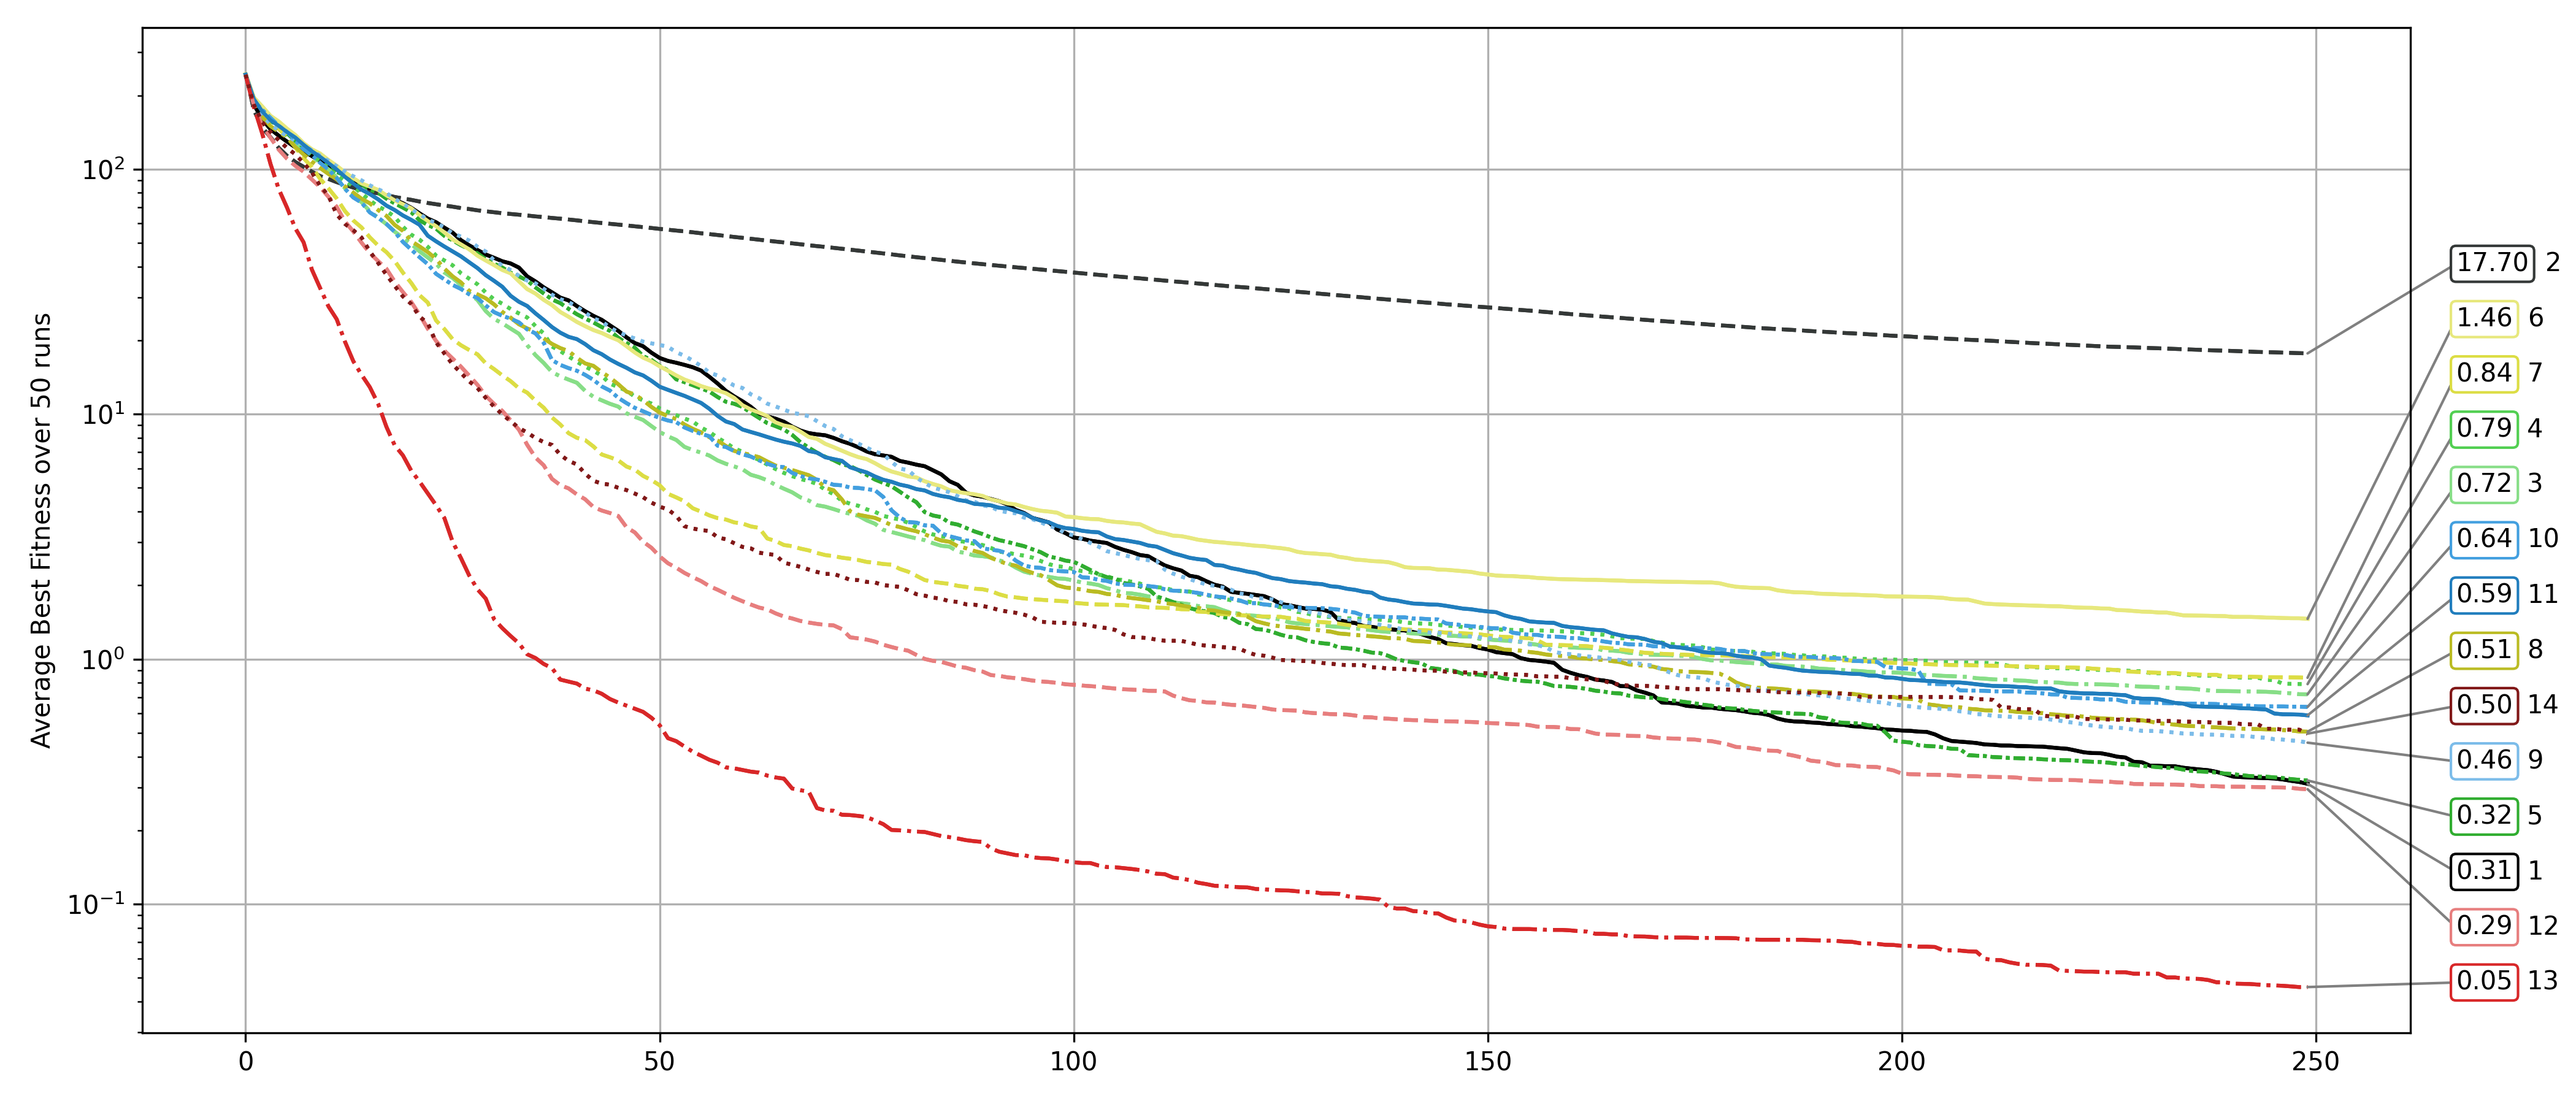
\includegraphics[width=.49\textwidth]{Figures/results/100/Alpine_N1_All_selected_algorithms_dim100_annot_legend.png}
    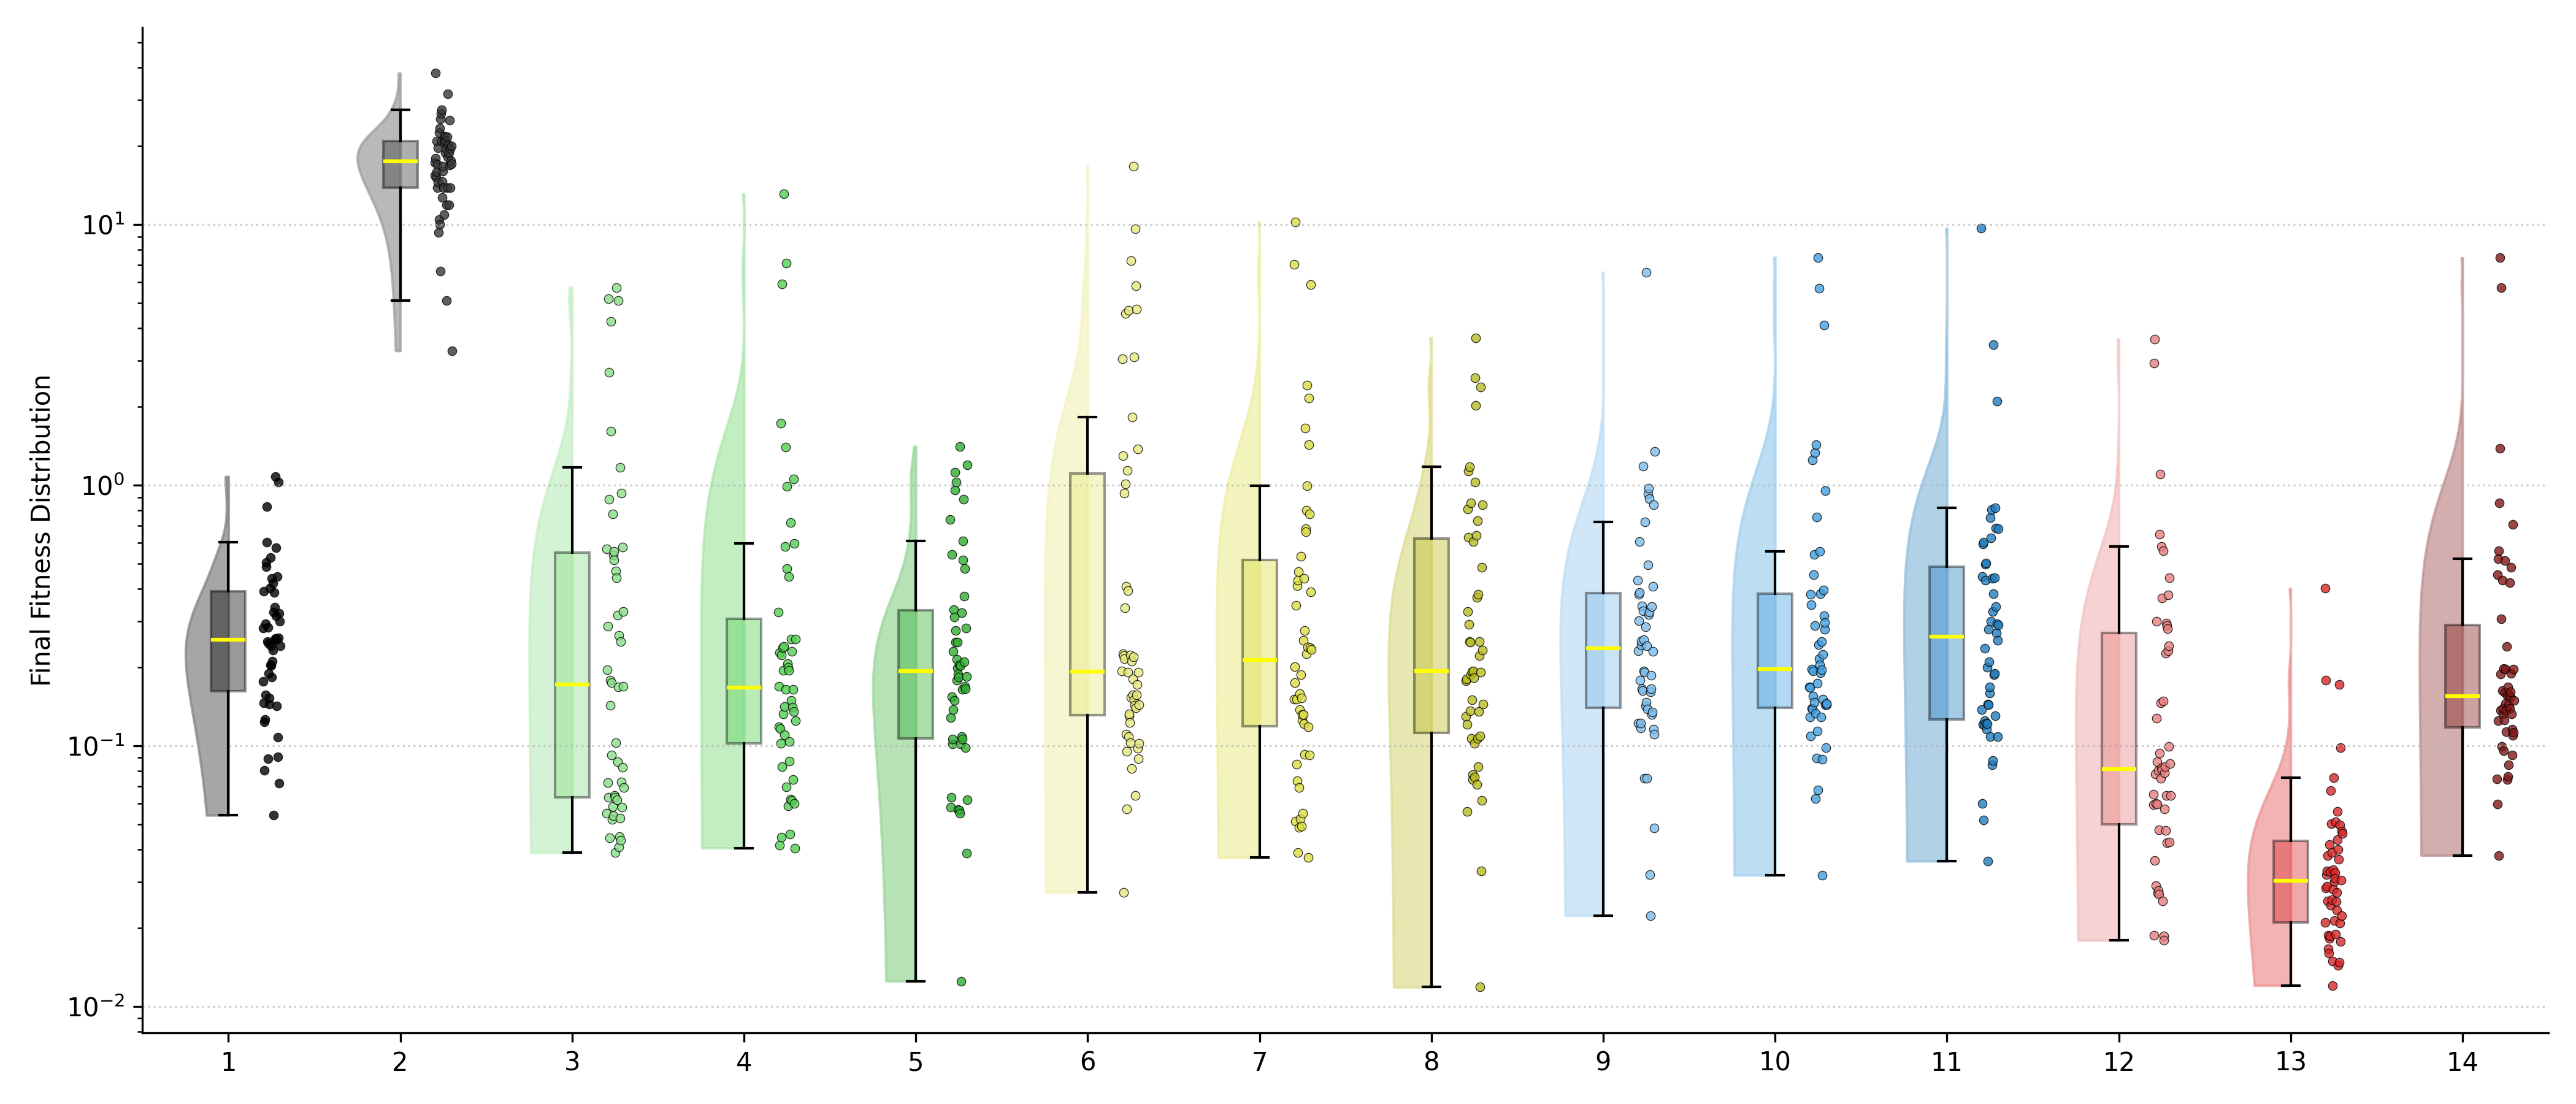
\includegraphics[width=.49\textwidth]{Figures/results/100/Alpine_N1_all_dim100_raincloud_vertical.png}
    \caption{Alpine N.1 (log)}
\end{subfigure}

\begin{subfigure}{1\textwidth}
    \centering
    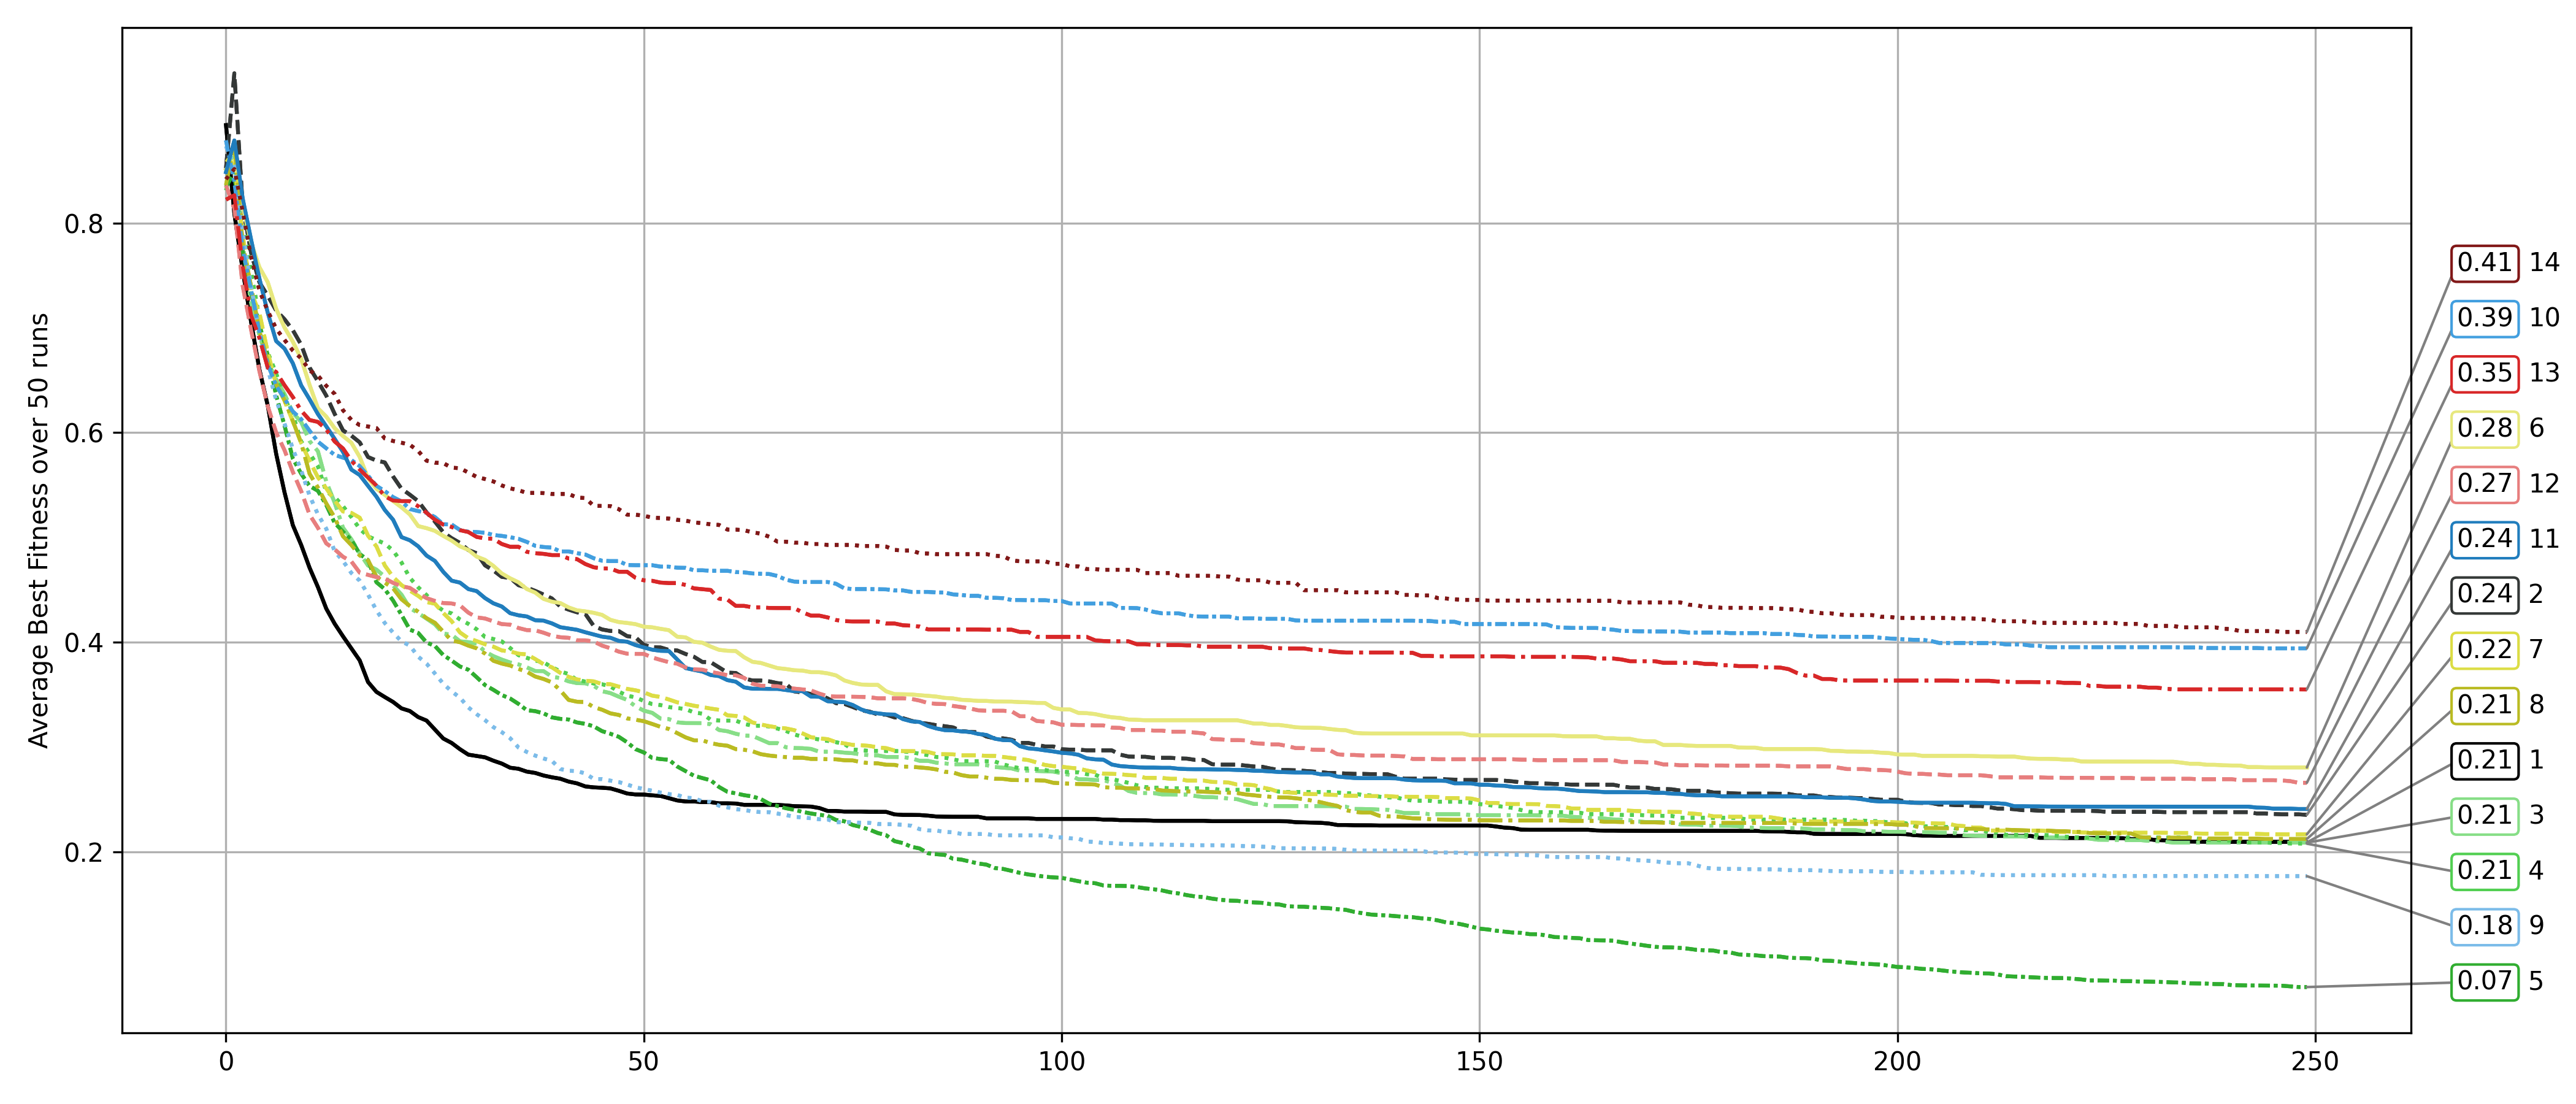
\includegraphics[width=.49\textwidth]{Figures/results/100/Crowned_Cross_All_selected_algorithms_dim100_annot_legend.png}
    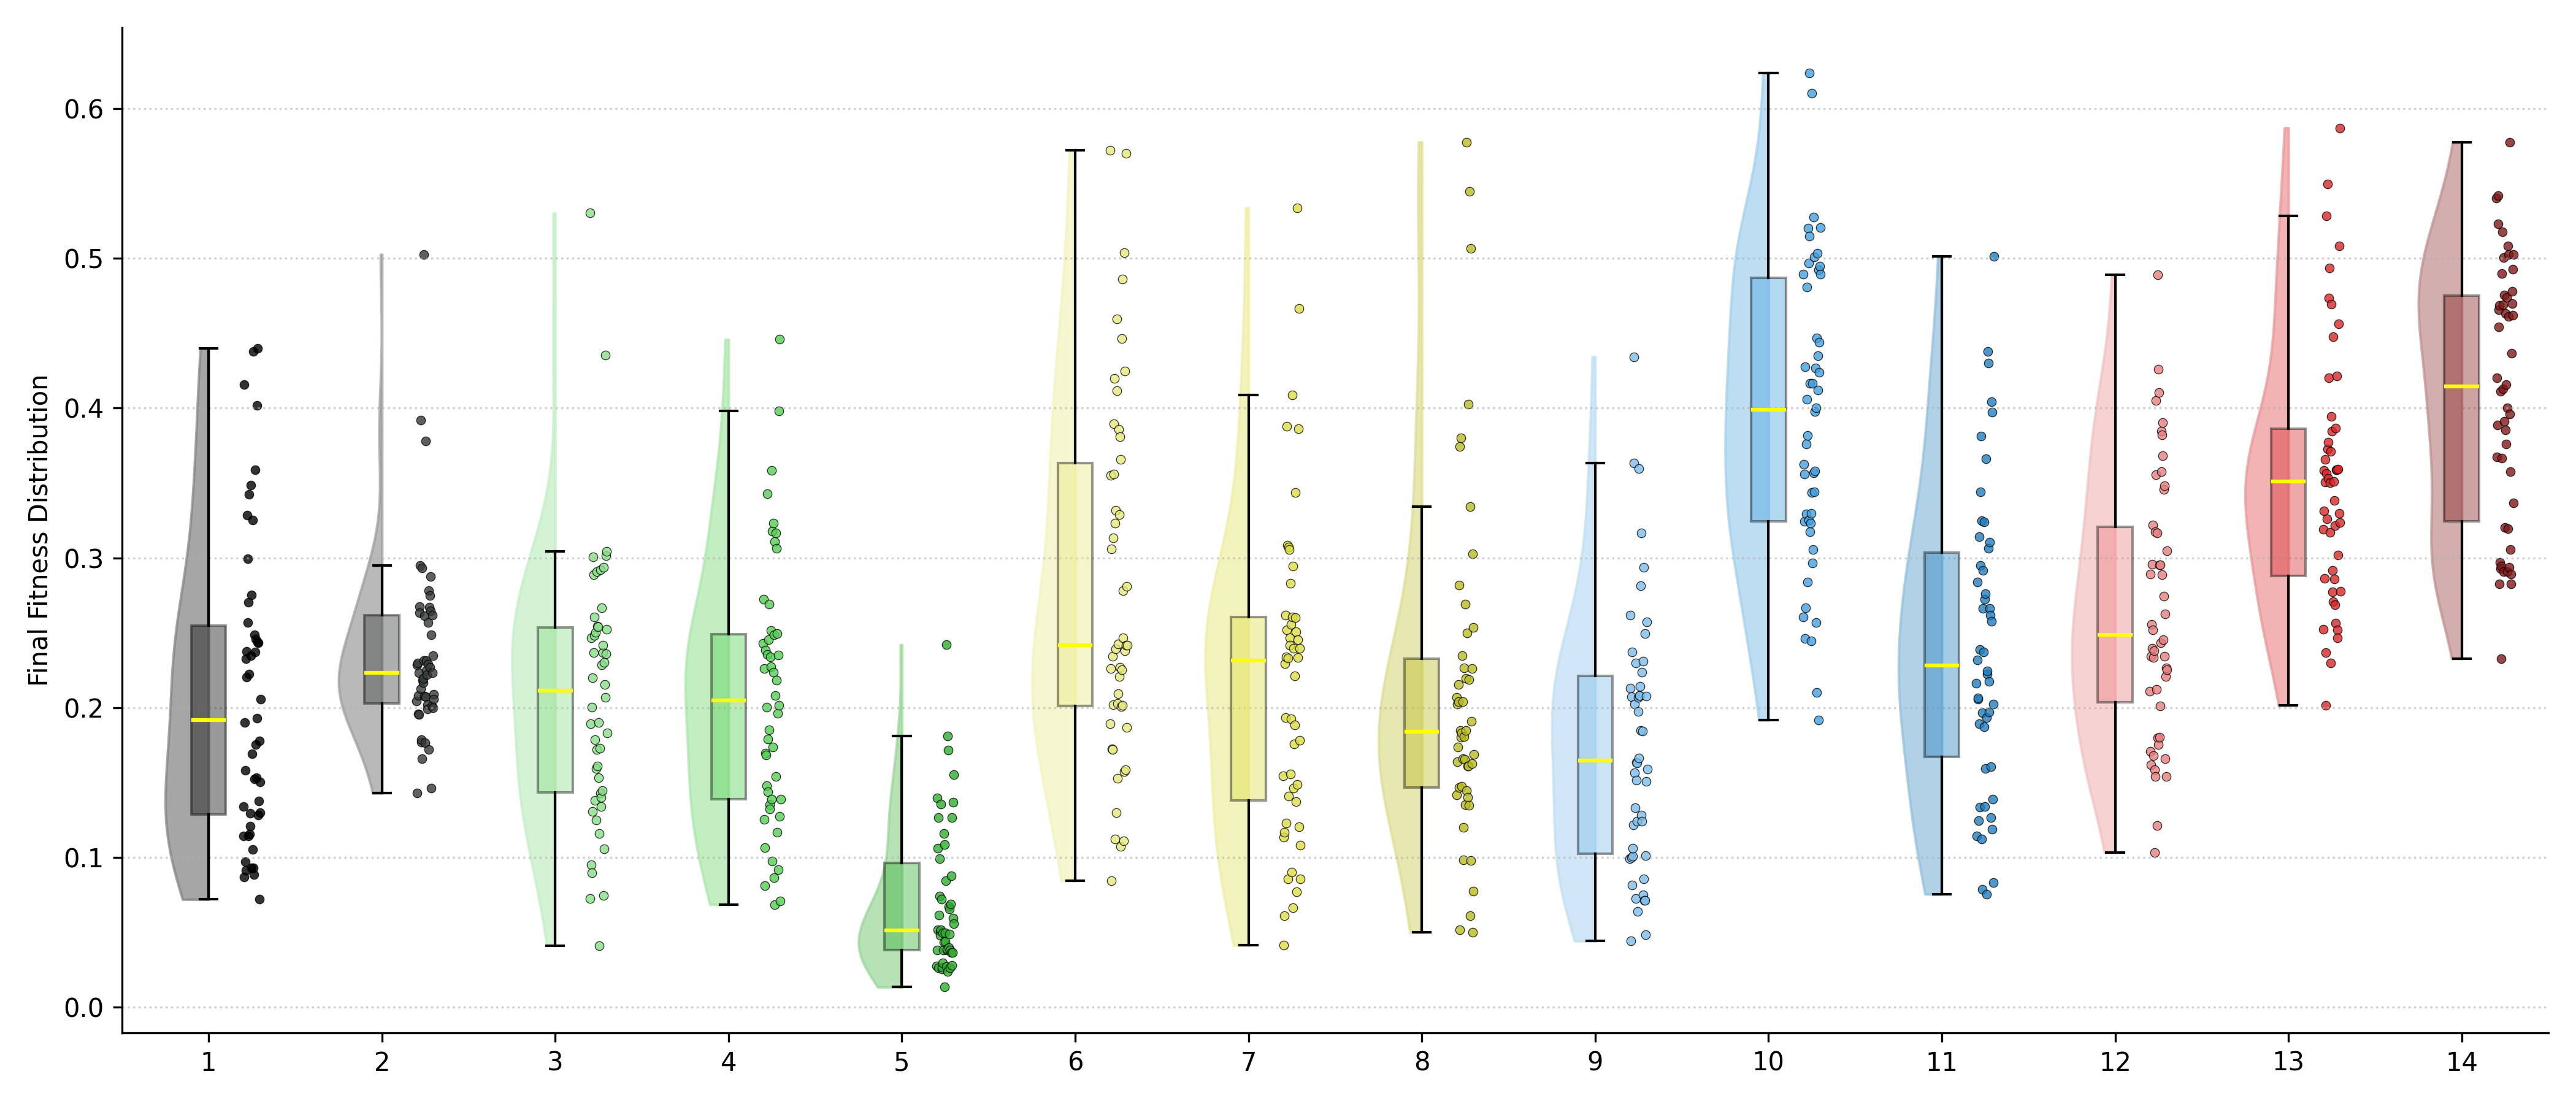
\includegraphics[width=.49\textwidth]{Figures/results/100/Crowned_Cross_all_dim100_raincloud_vertical.png}
    \caption{Crowned Cross}
\end{subfigure}

\begin{subfigure}{1\textwidth}
    \centering
    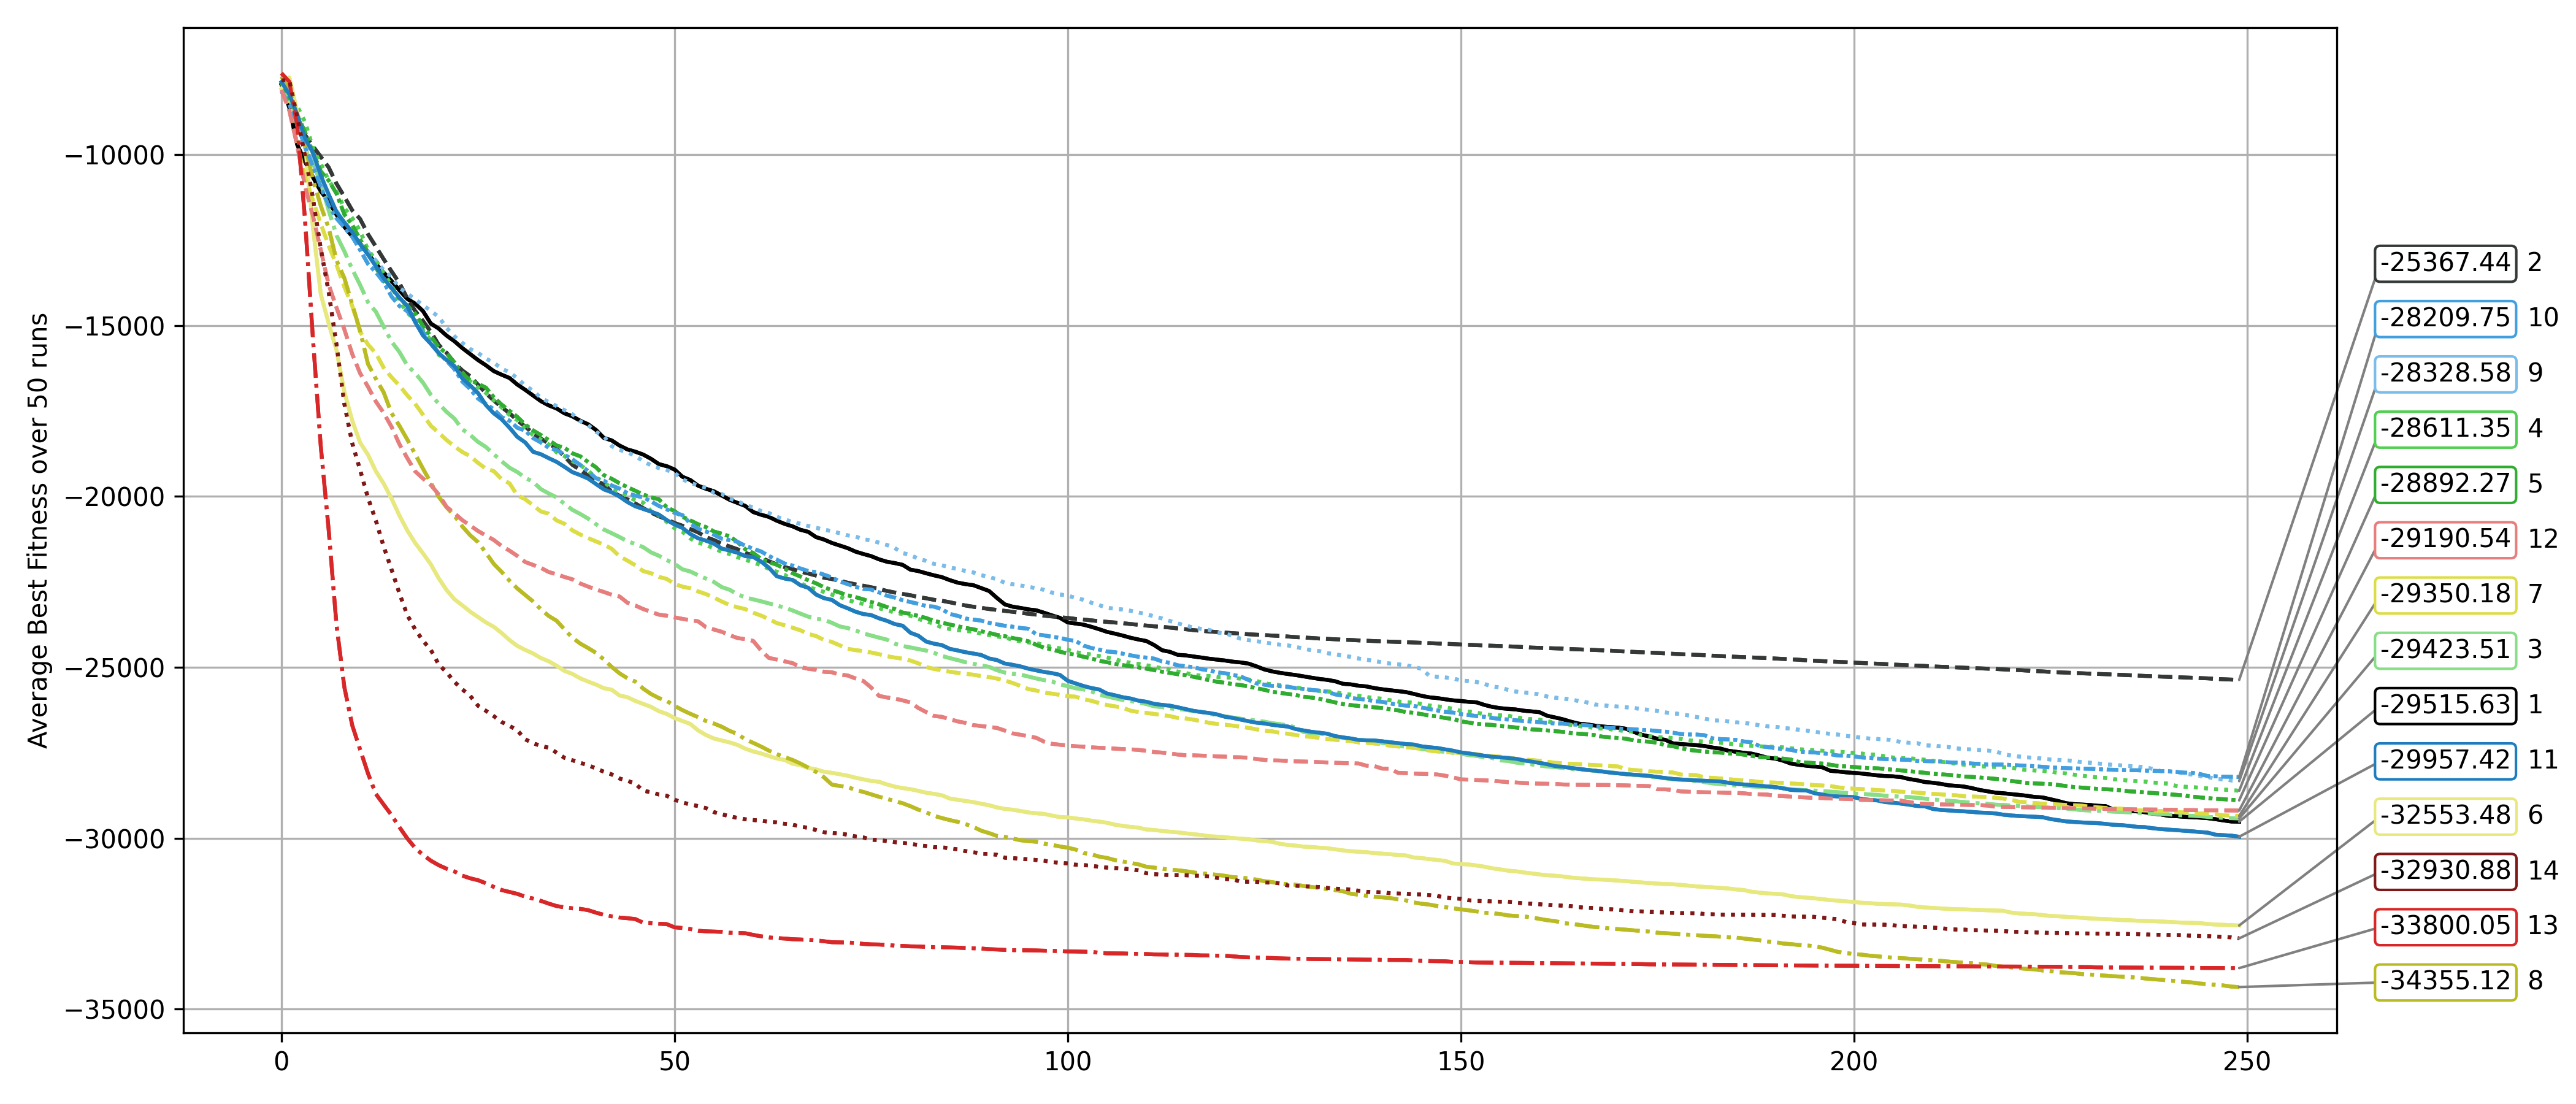
\includegraphics[width=.49\textwidth]{Figures/results/100/Egg_Holder_All_selected_algorithms_dim100_annot_legend.png}
    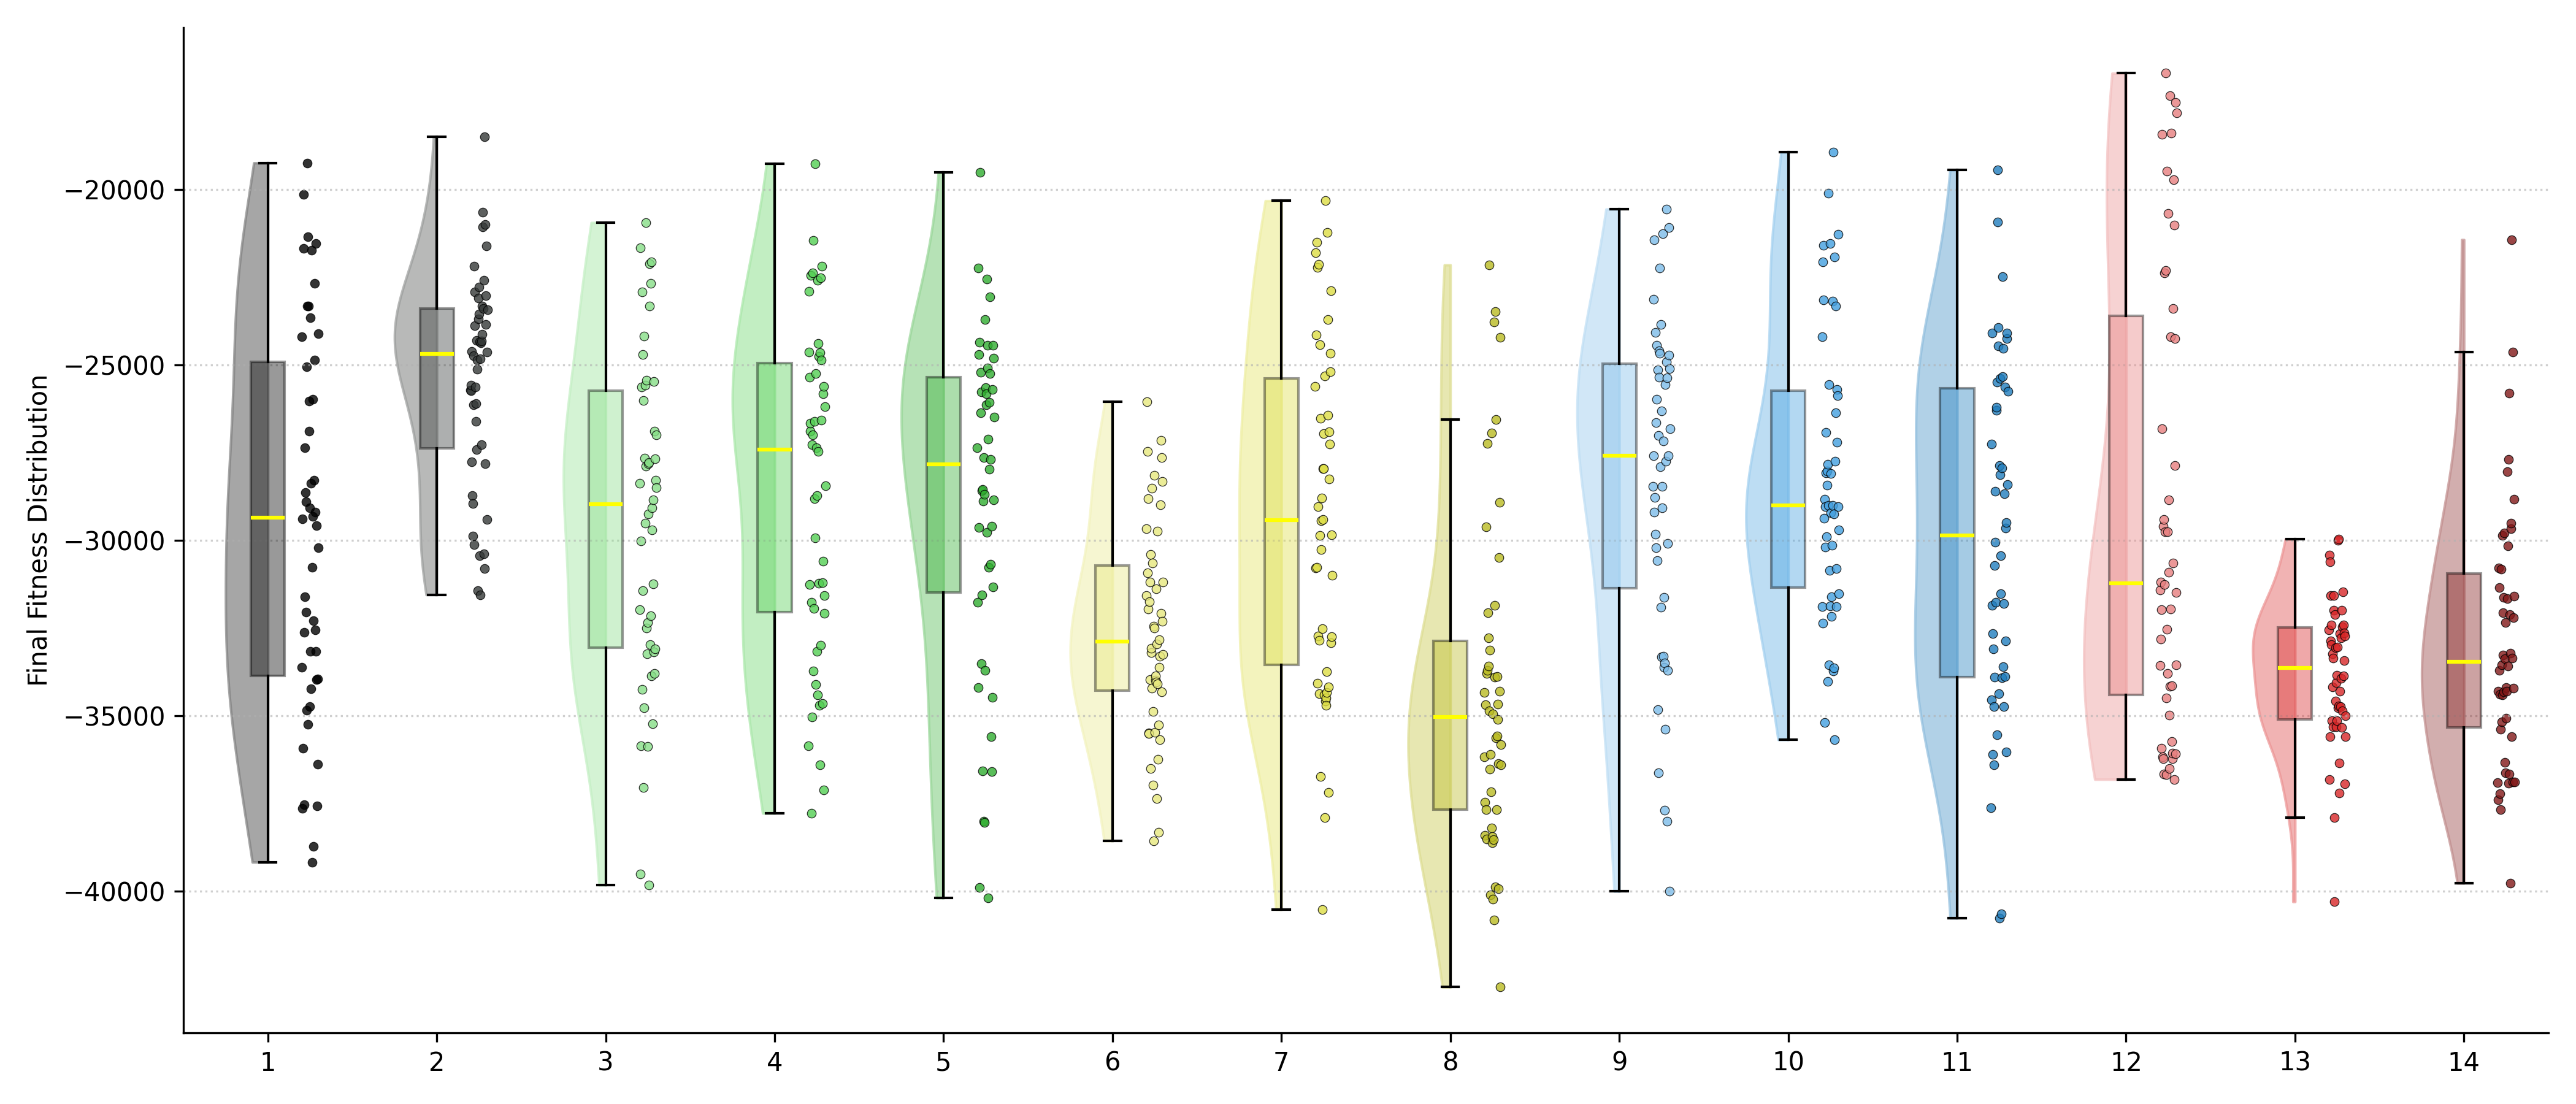
\includegraphics[width=.49\textwidth]{Figures/results/100/Egg_Holder_all_dim100_raincloud_vertical.png}
    \caption{Egg-Holder}
\end{subfigure}

\begin{subfigure}{1\textwidth}
    \centering
    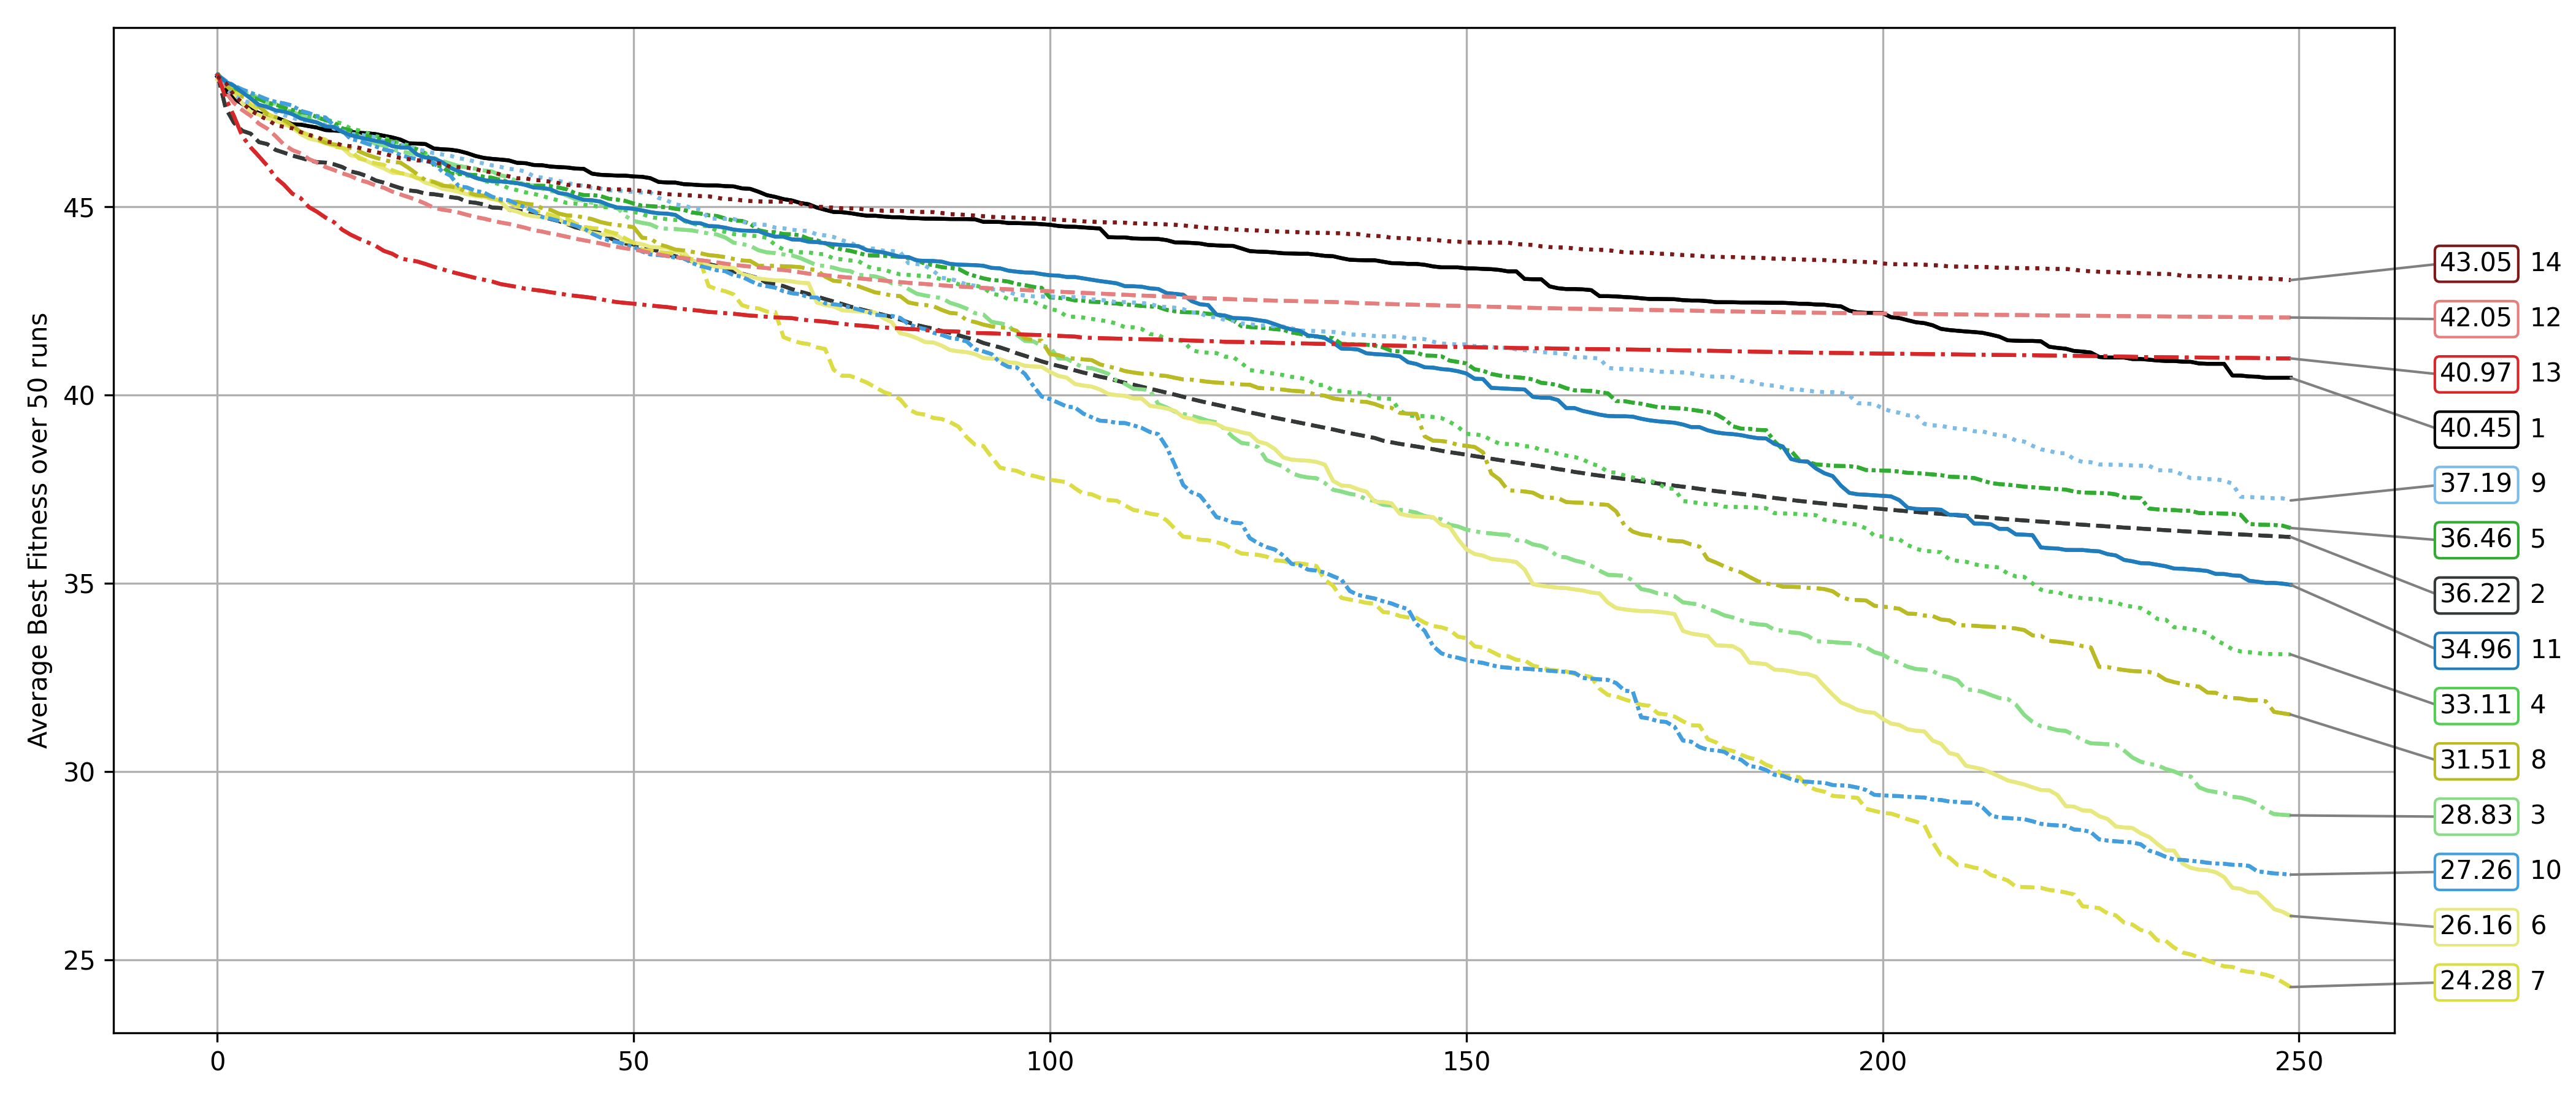
\includegraphics[width=.49\textwidth]{Figures/results/100/Expanded_Shaffer_All_selected_algorithms_dim100_annot_legend.png}
    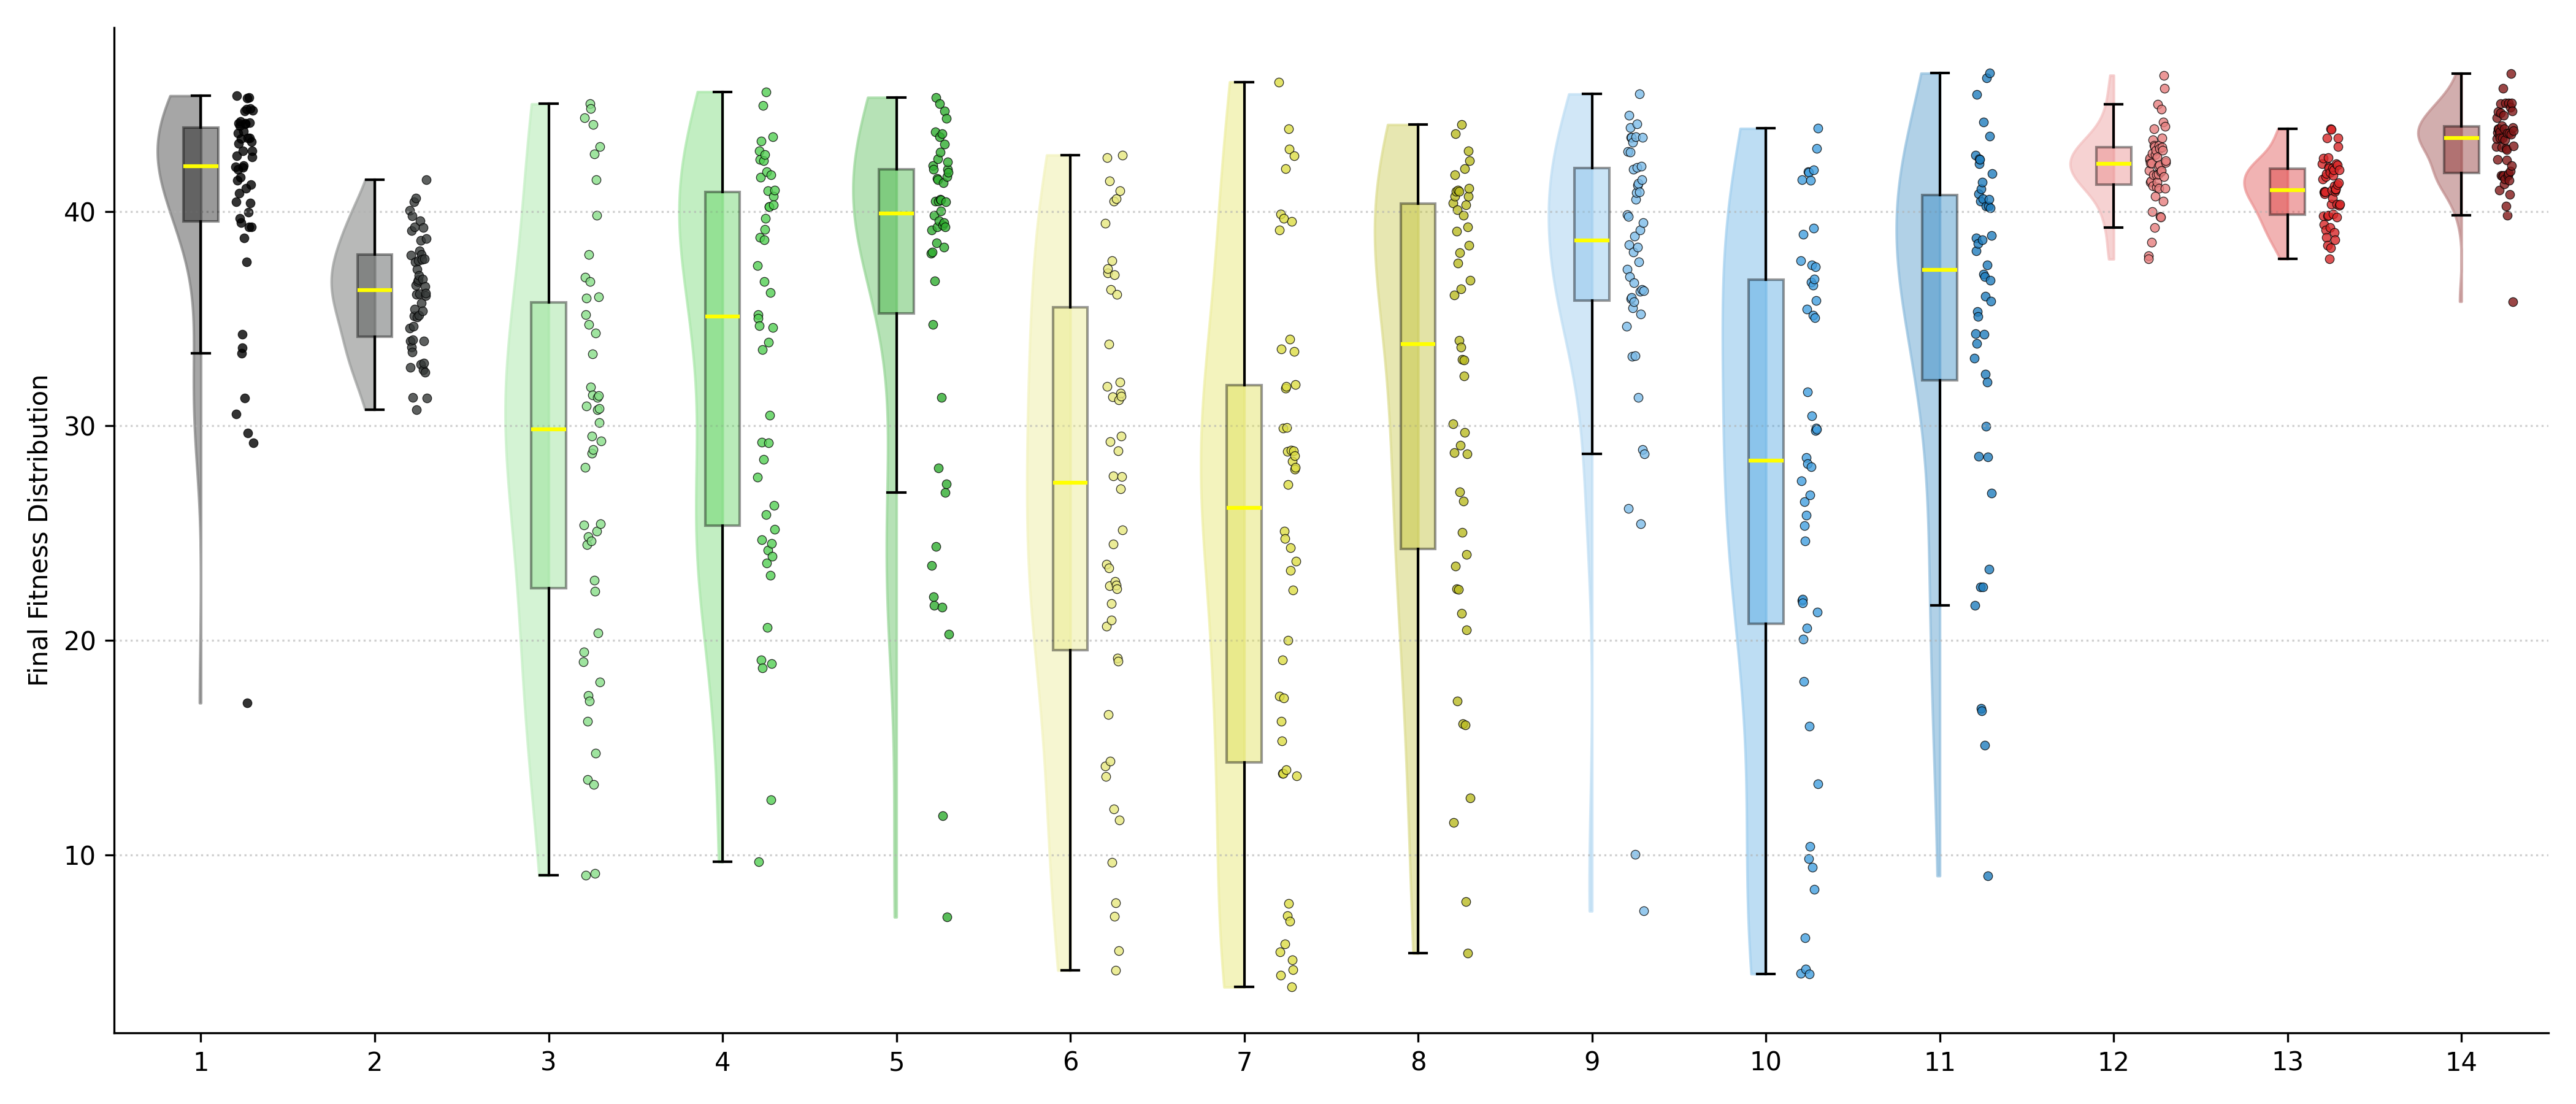
\includegraphics[width=.49\textwidth]{Figures/results/100/Expanded_Shaffer_all_dim100_raincloud_vertical.png}
    \caption{Expanded Shaffer}
\end{subfigure}

\begin{subfigure}{1\textwidth}
    \centering
    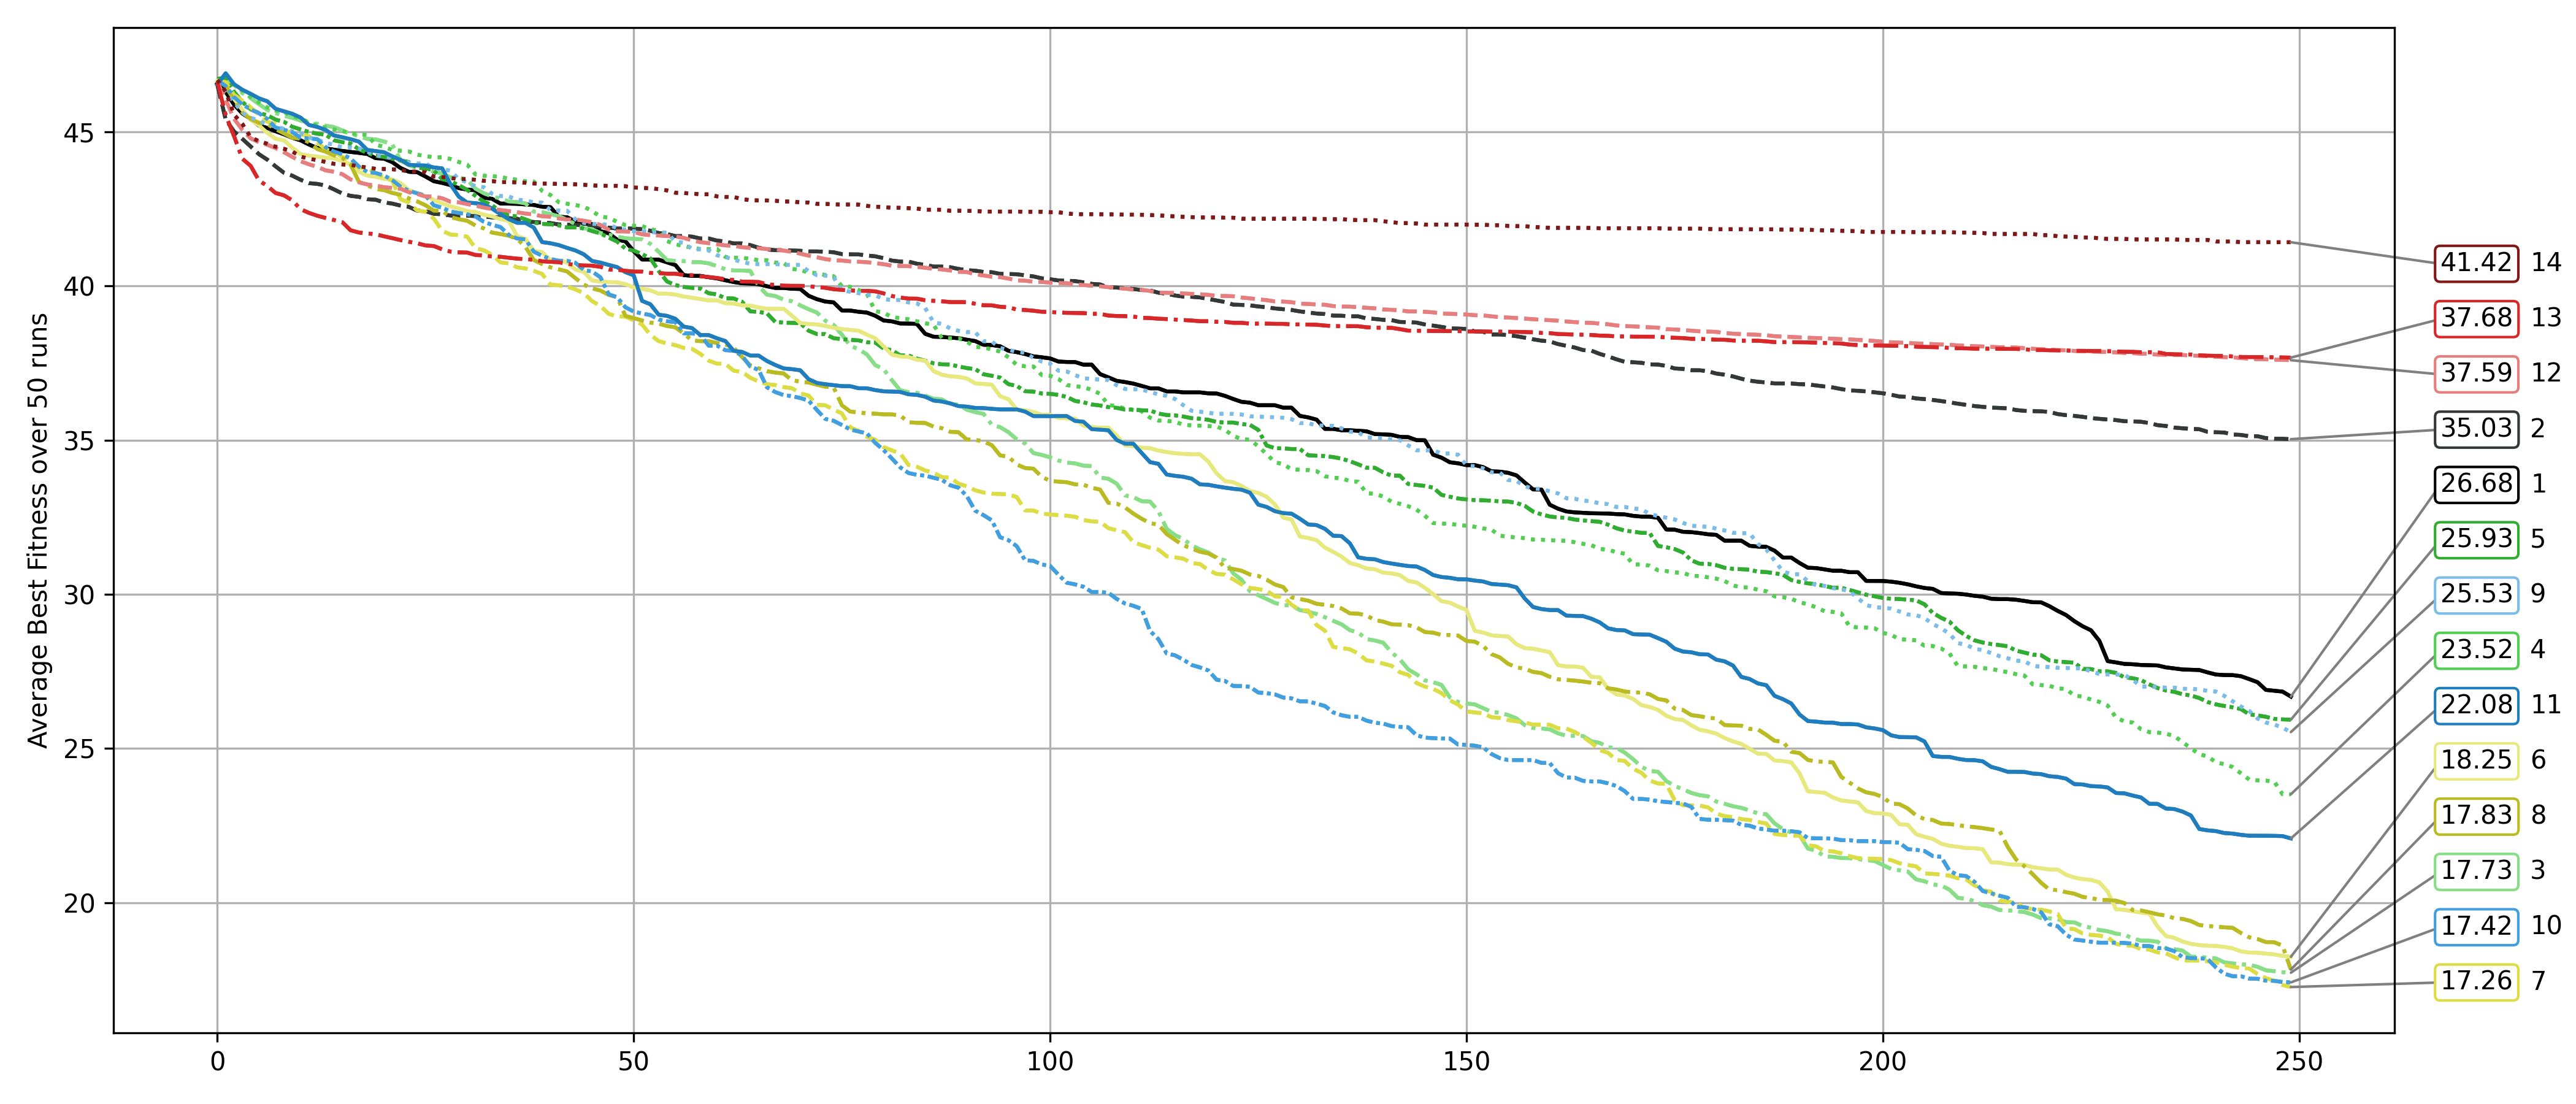
\includegraphics[width=.49\textwidth]{Figures/results/100/Generalized_Schaffer_N1_All_selected_algorithms_dim100_annot_legend.png}
    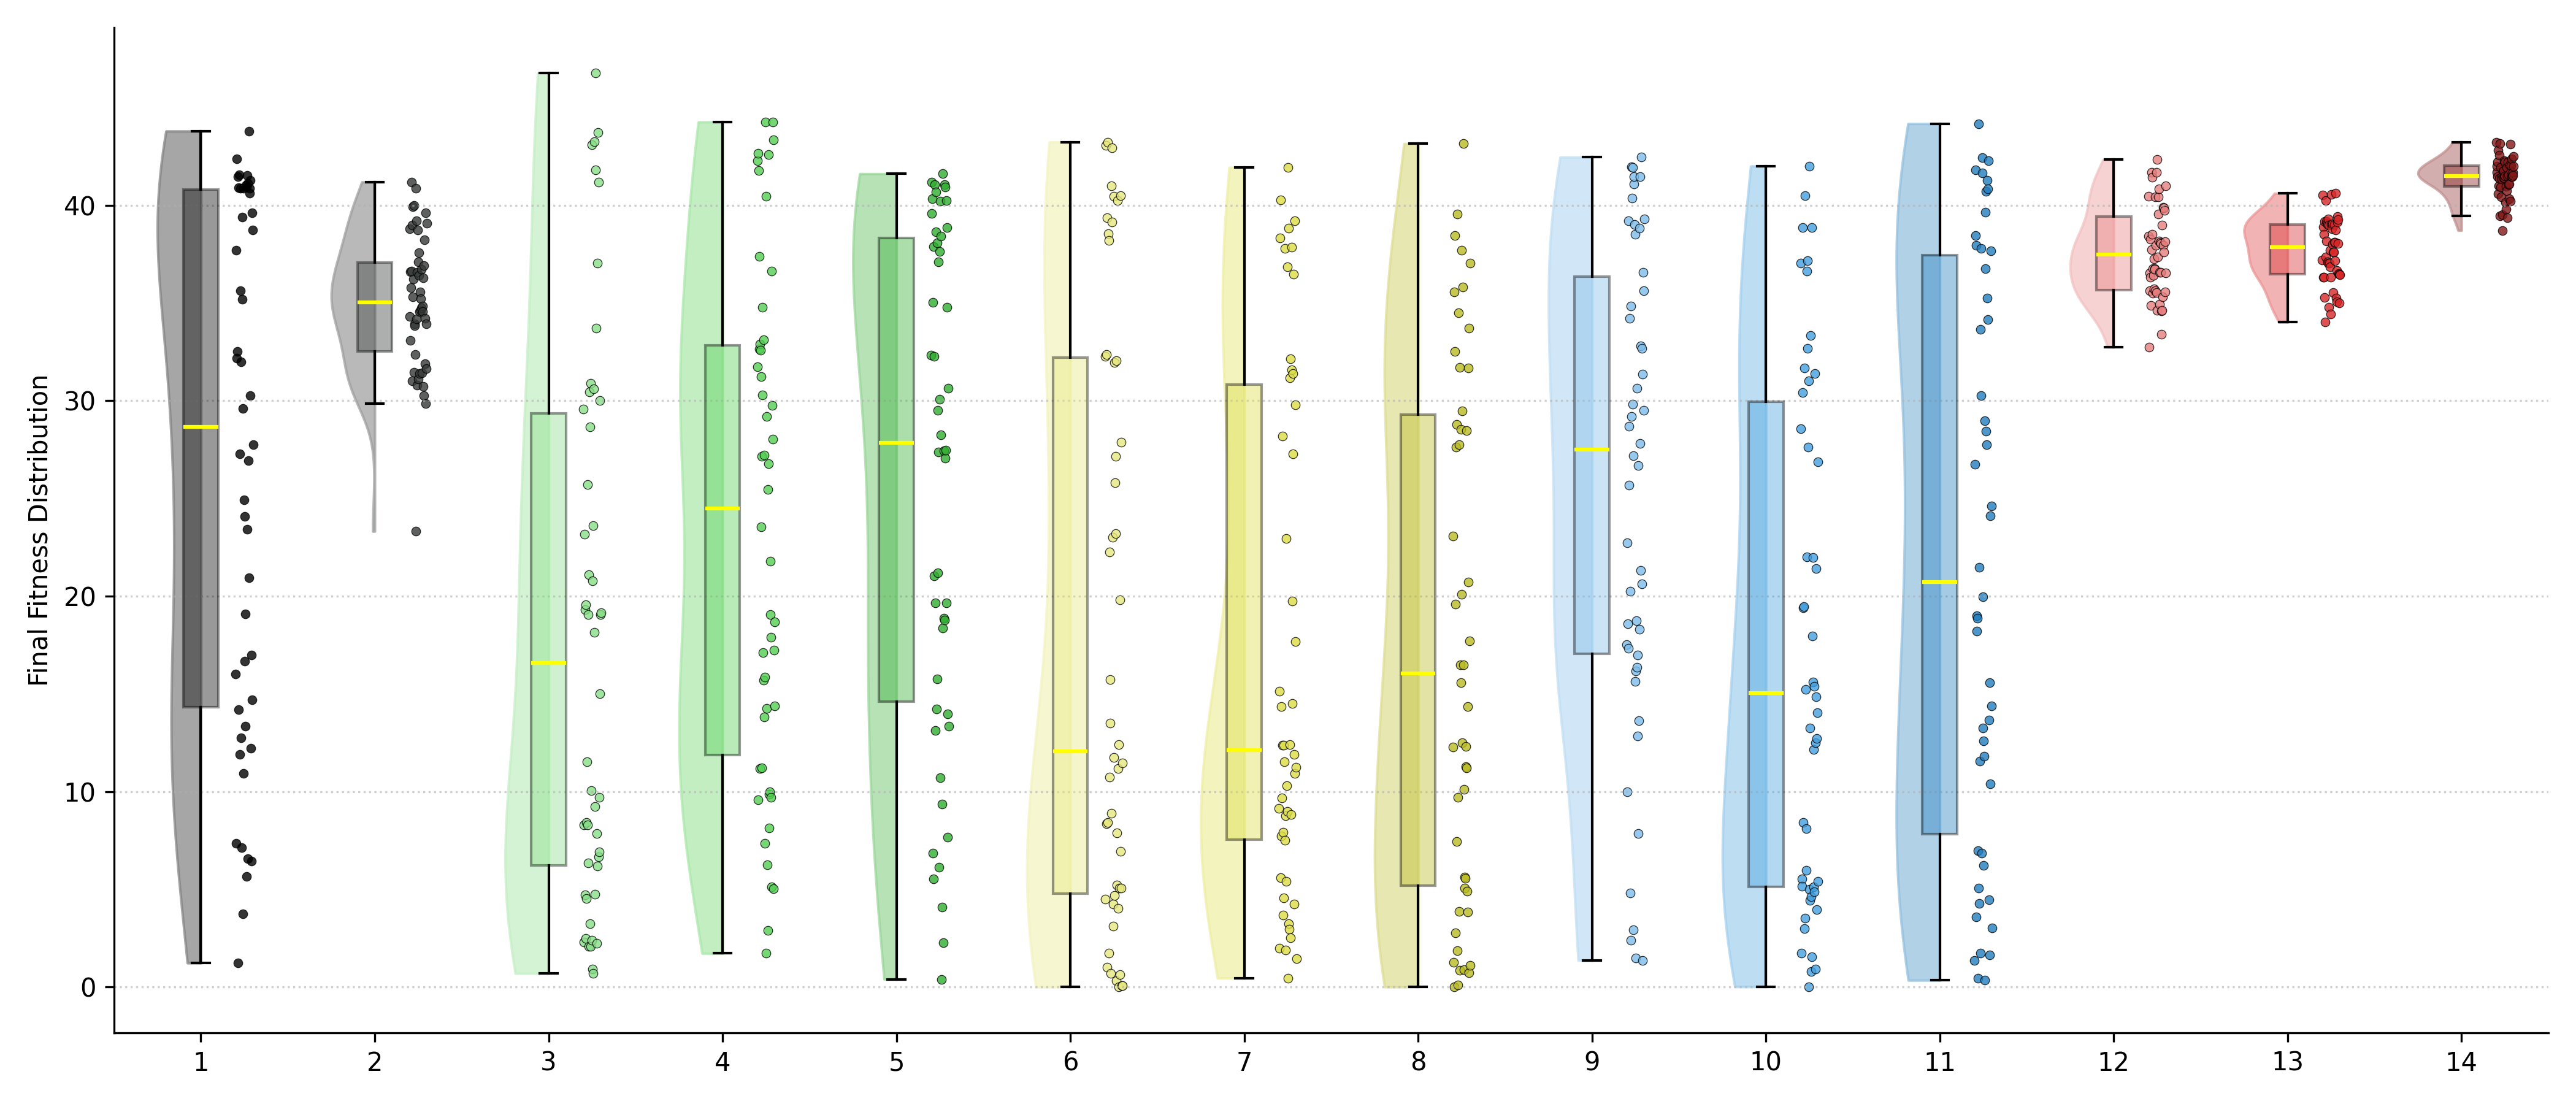
\includegraphics[width=.49\textwidth]{Figures/results/100/Generalized_Schaffer_N1_all_dim100_raincloud_vertical.png}
    \caption{Generalized Schaffer N.1}
\end{subfigure}

\begin{subfigure}{1\textwidth}
    \centering
    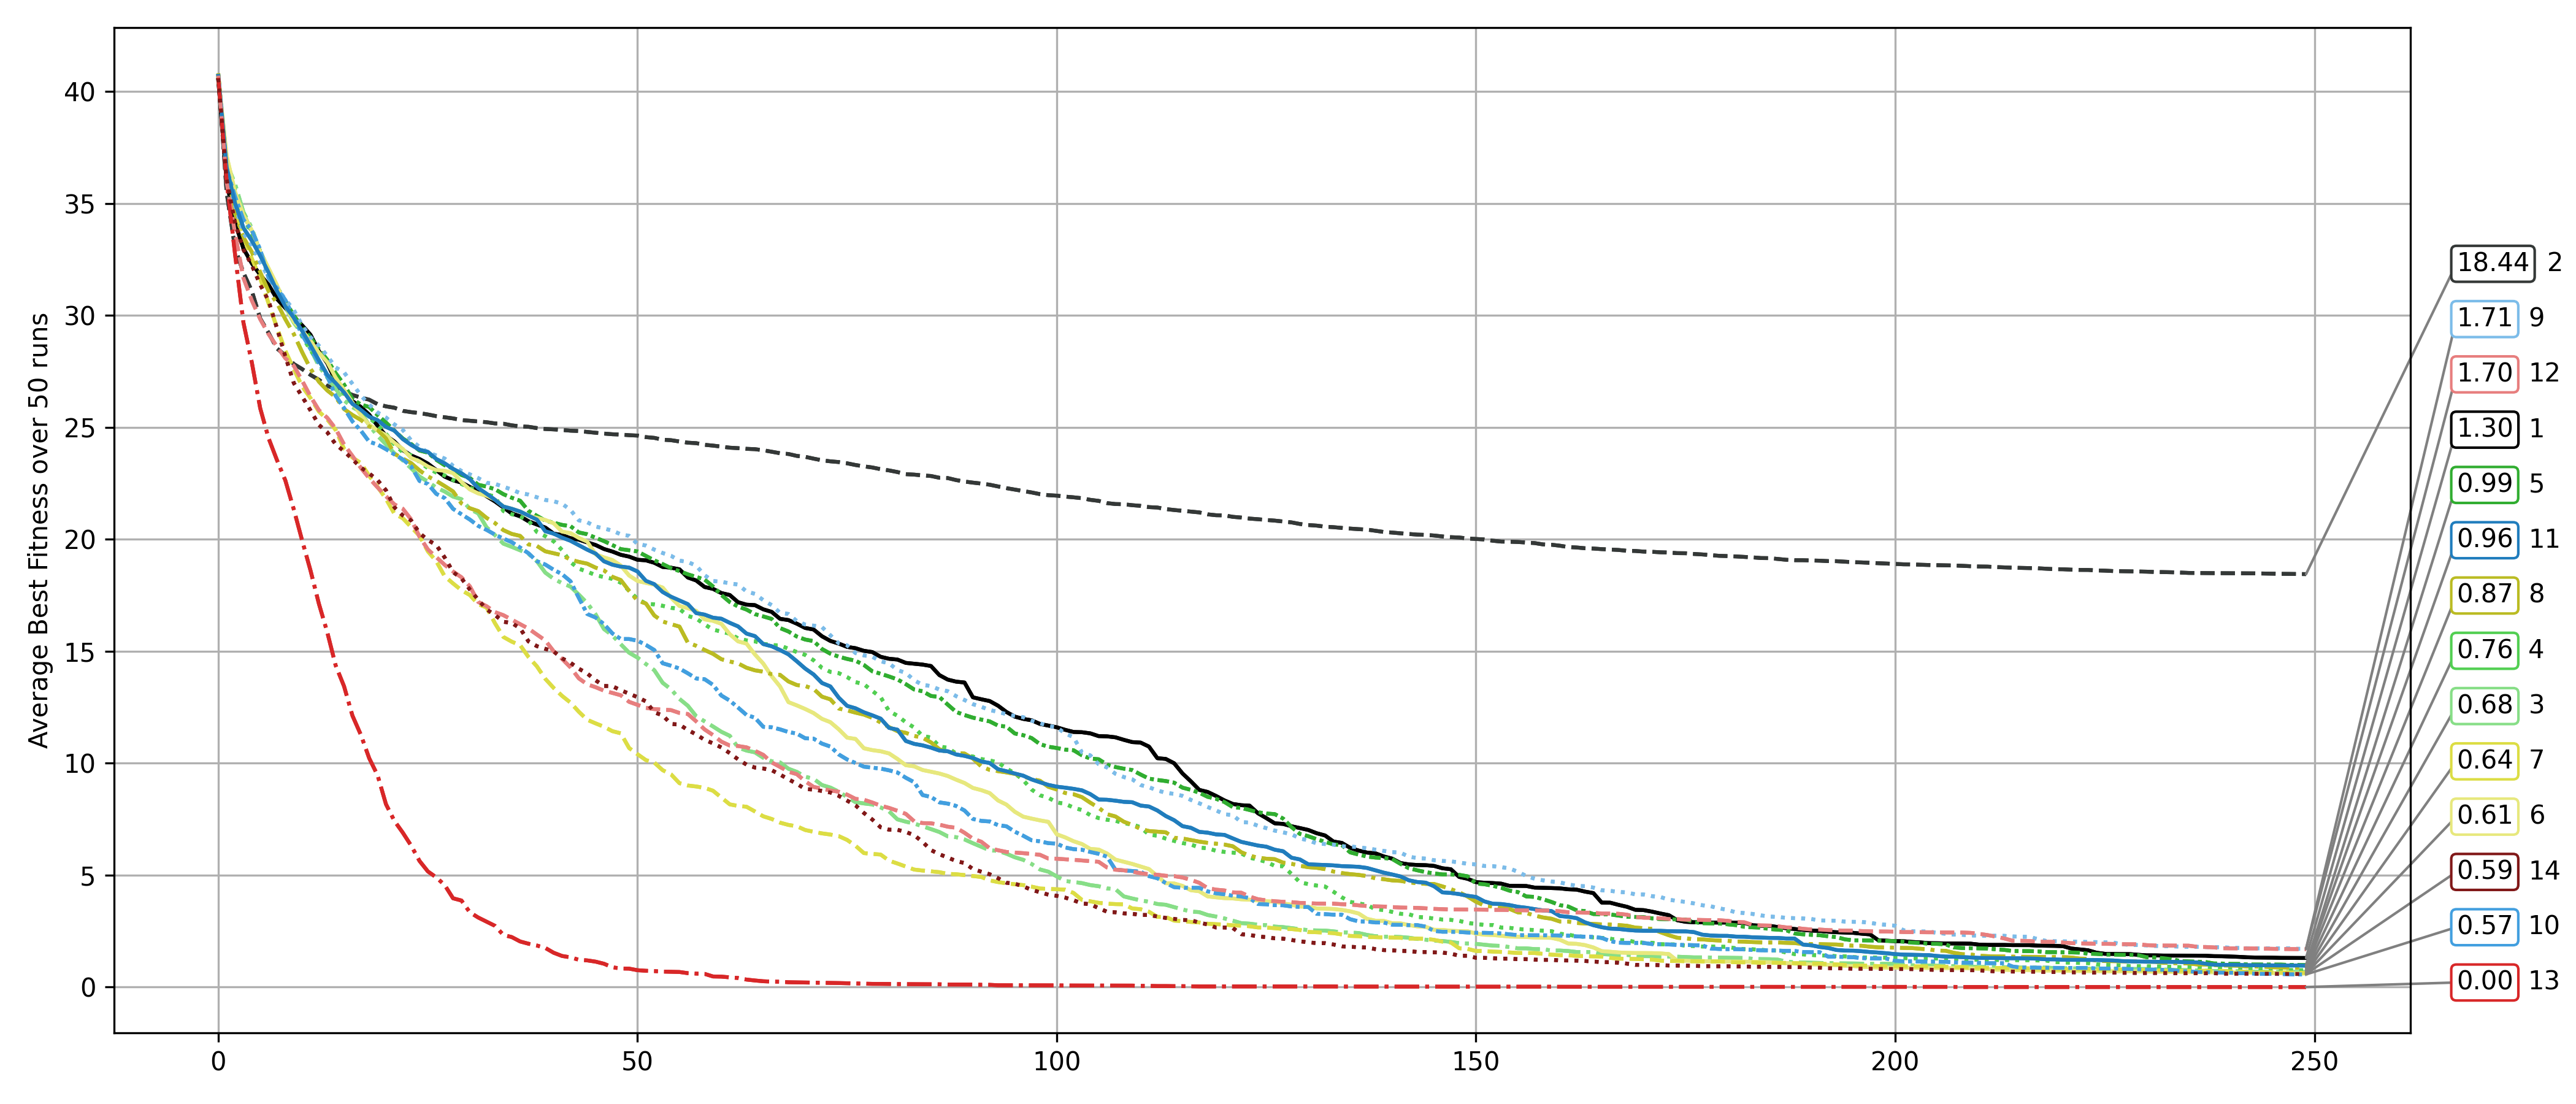
\includegraphics[width=.49\textwidth]{Figures/results/100/Generalized_Schaffer_N2_All_selected_algorithms_dim100_annot_legend.png}
    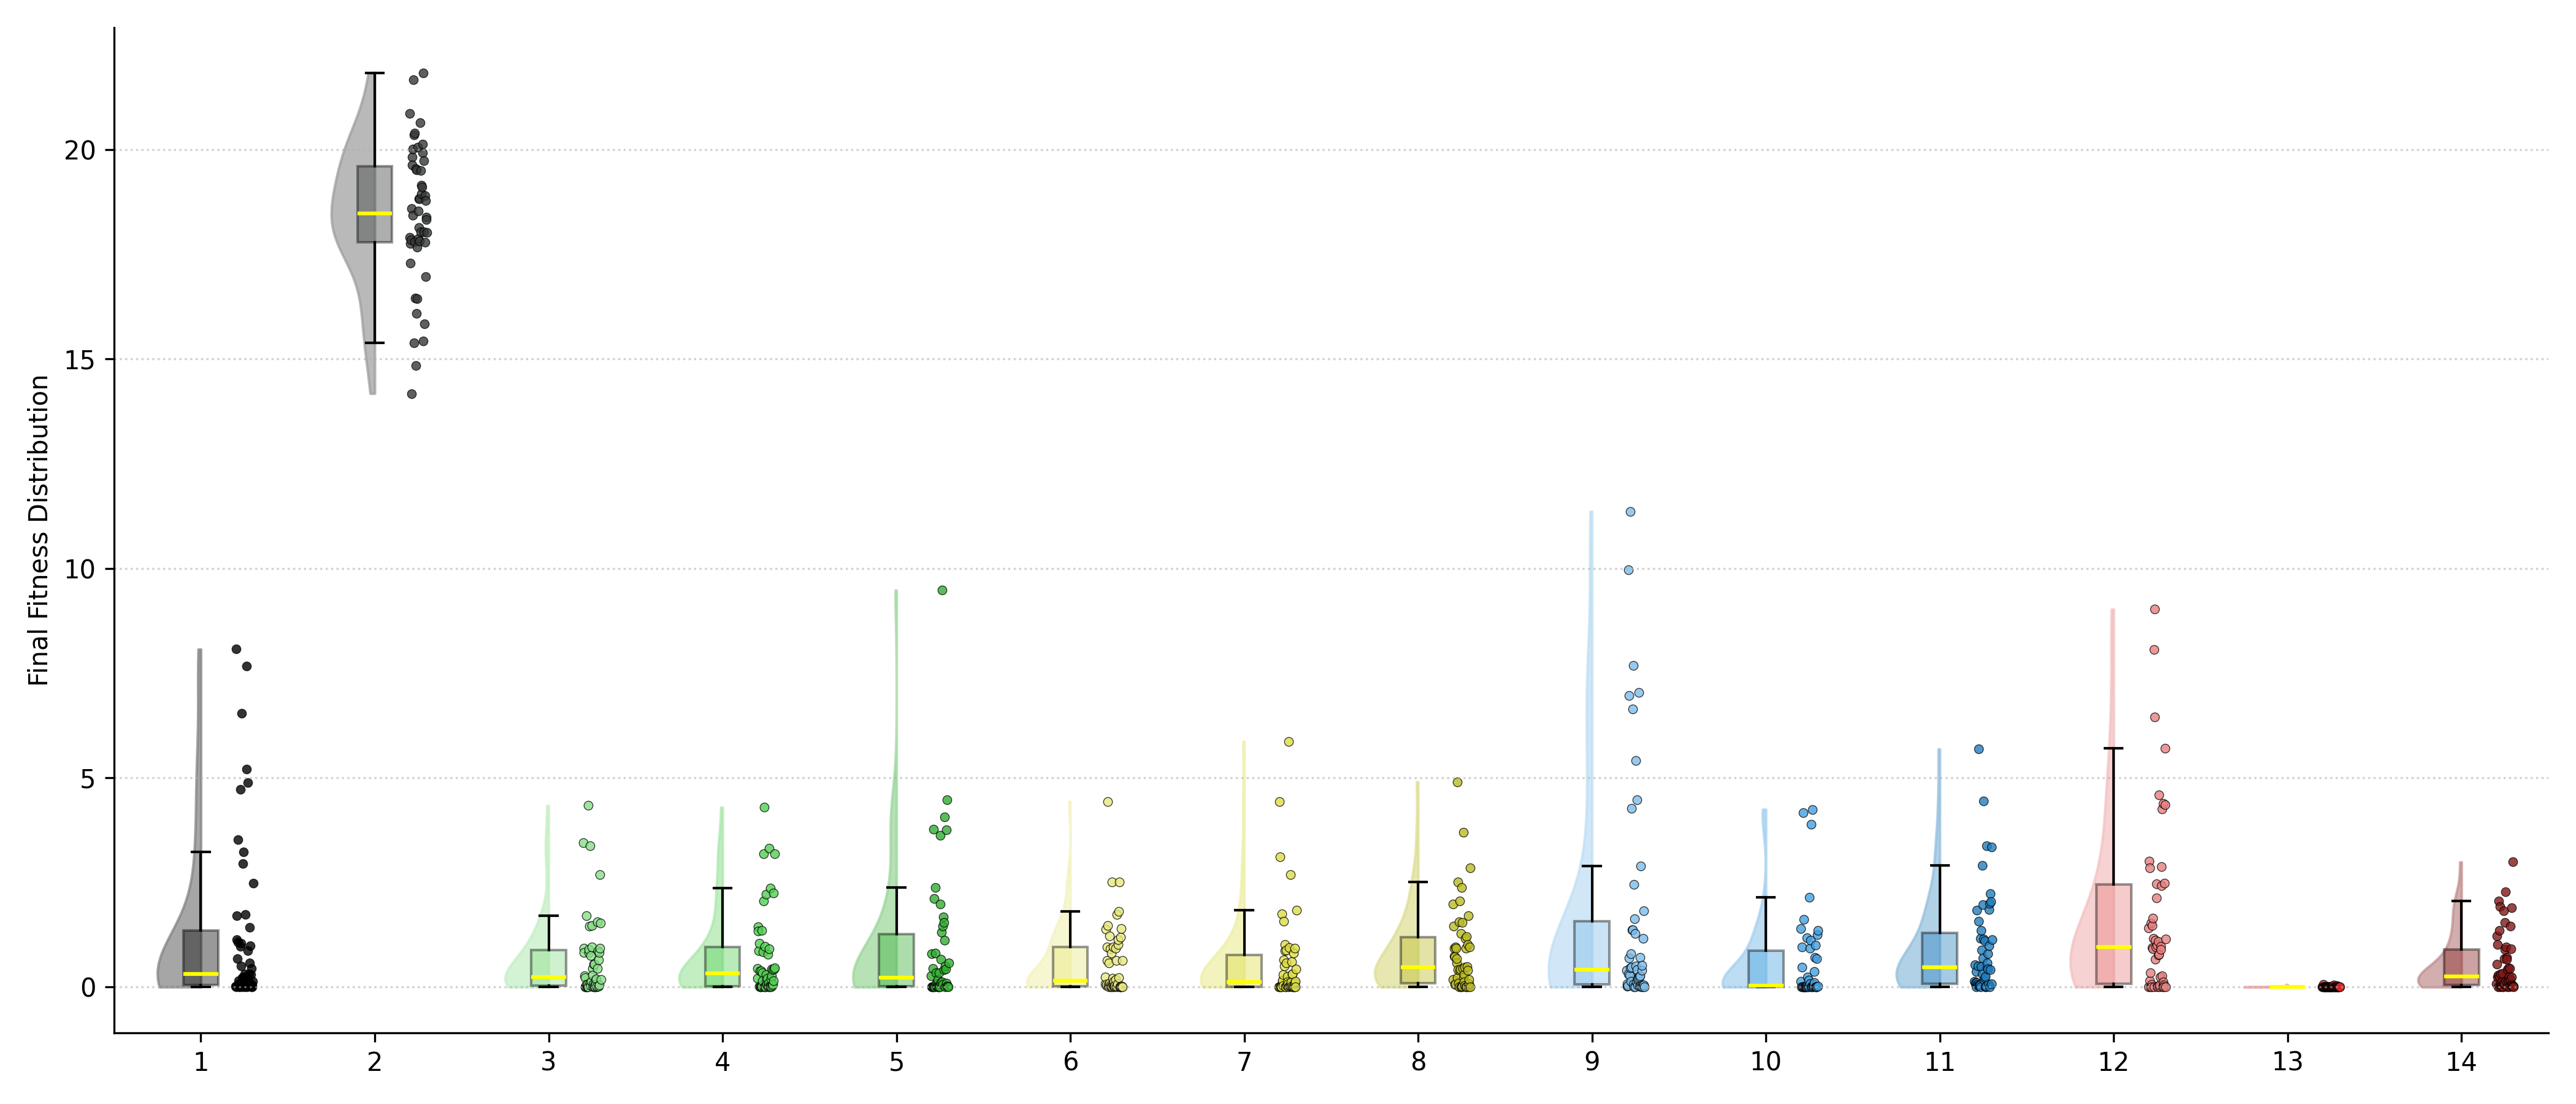
\includegraphics[width=.49\textwidth]{Figures/results/100/Generalized_Schaffer_N2_all_dim100_raincloud_vertical.png}
    \caption{Generalized Schaffer N.2}
\end{subfigure}

% \enlargethispage{3\baselineskip}
            \captionsetup{list=no}
\caption[Convergence curves and final fitness distribution raincloud plots for 100-dimensional problems]{Convergence curves (left) and final fitness distribution raincloud plots (right) for each tested benchmark problem in the 100-dimensional setting. Algorithms are numbered, line-styled, ordered, and color-coded consistently according to the legend in Figure~\ref{fig:plot_encoding}. Problems plotted on a logarithmic scale are indicated with ``(log)'' following the problem name.}

\end{figure}




%%%%%%%%%%%%%%%%%%%%%%%%%%%




\begin{figure}[p]\ContinuedFloat
\renewcommand\thesubfigure{C.\arabic{figure}.\arabic{subfigure}} % Local change starts here

    \centering

\begin{subfigure}{1\textwidth}
    \centering
    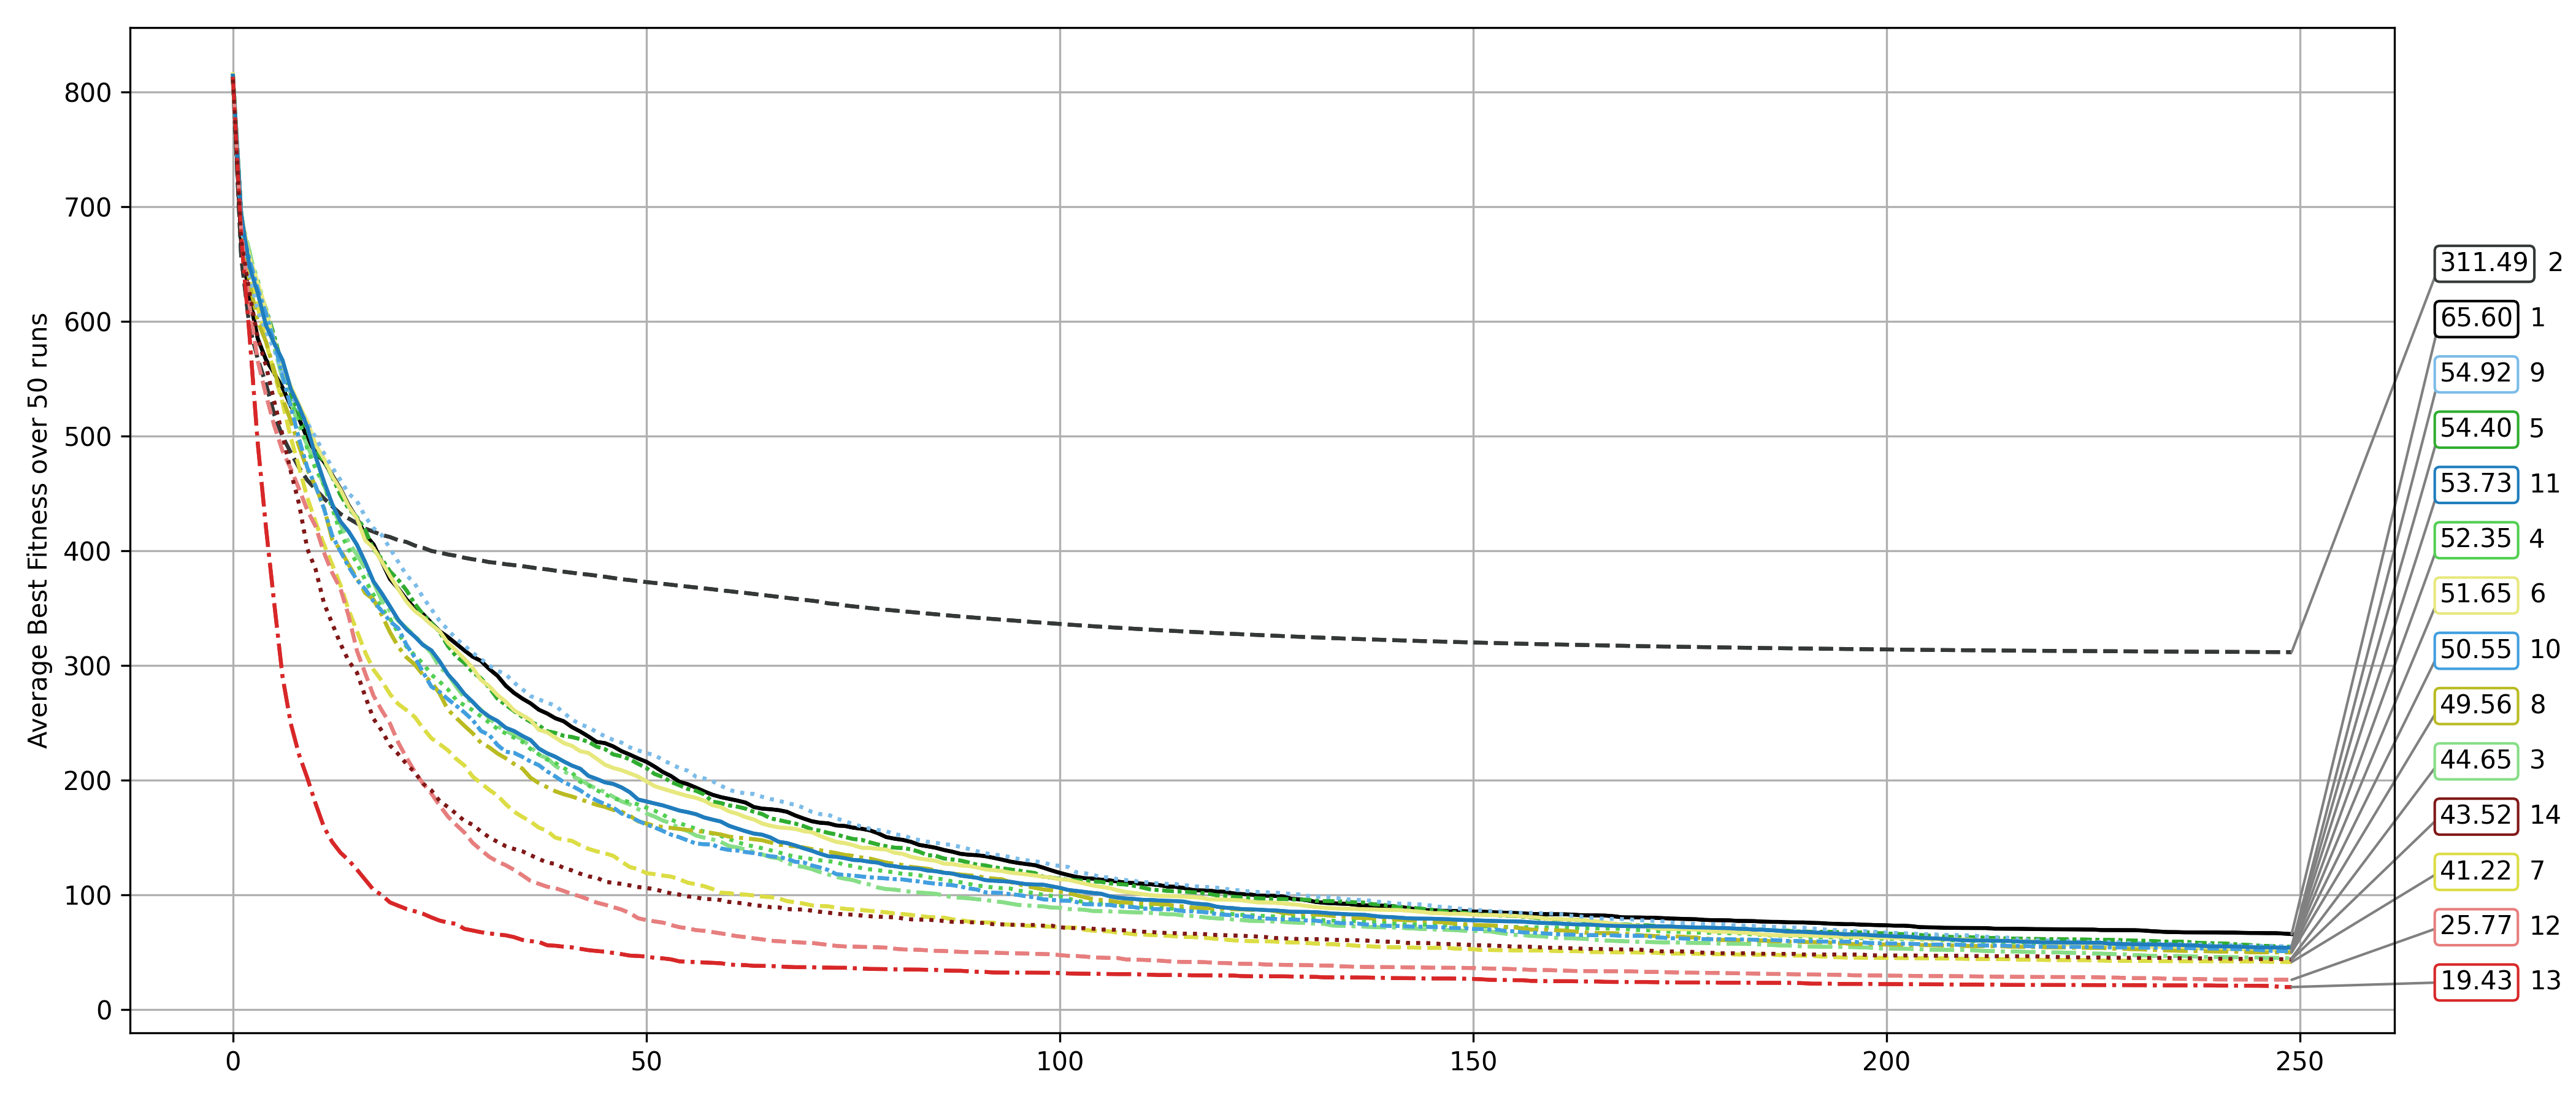
\includegraphics[width=.49\textwidth]{Figures/results/100/Generalized_Schaffer_N3_All_selected_algorithms_dim100_annot_legend.png}
    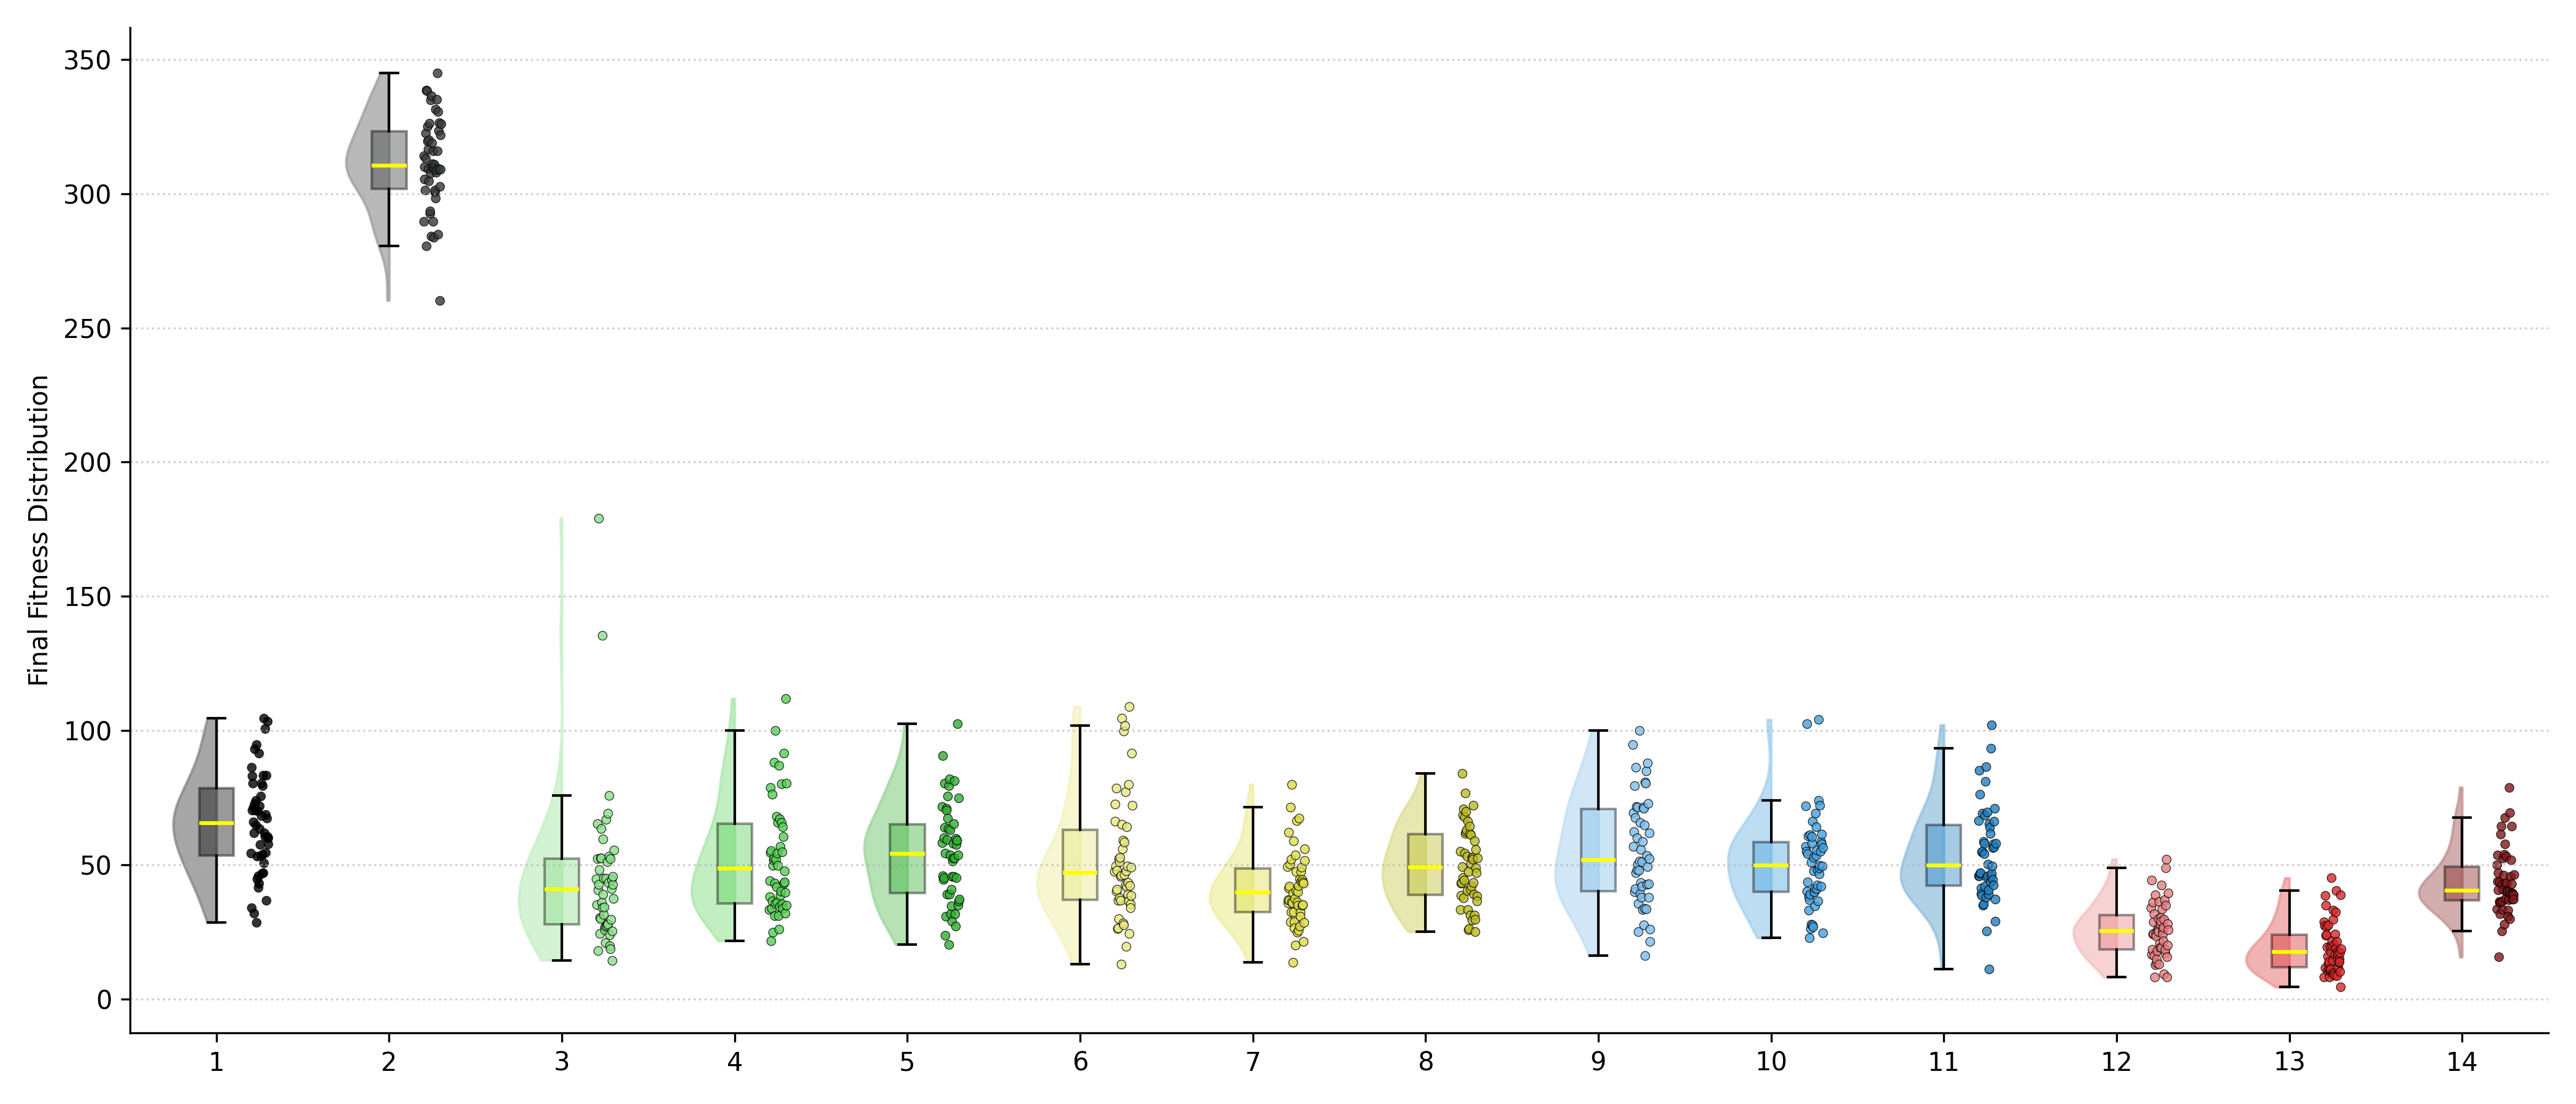
\includegraphics[width=.49\textwidth]{Figures/results/100/Generalized_Schaffer_N3_all_dim100_raincloud_vertical.png}
    \caption{Generalized Schaffer N3}
\end{subfigure}

\begin{subfigure}{1\textwidth}
    \centering
    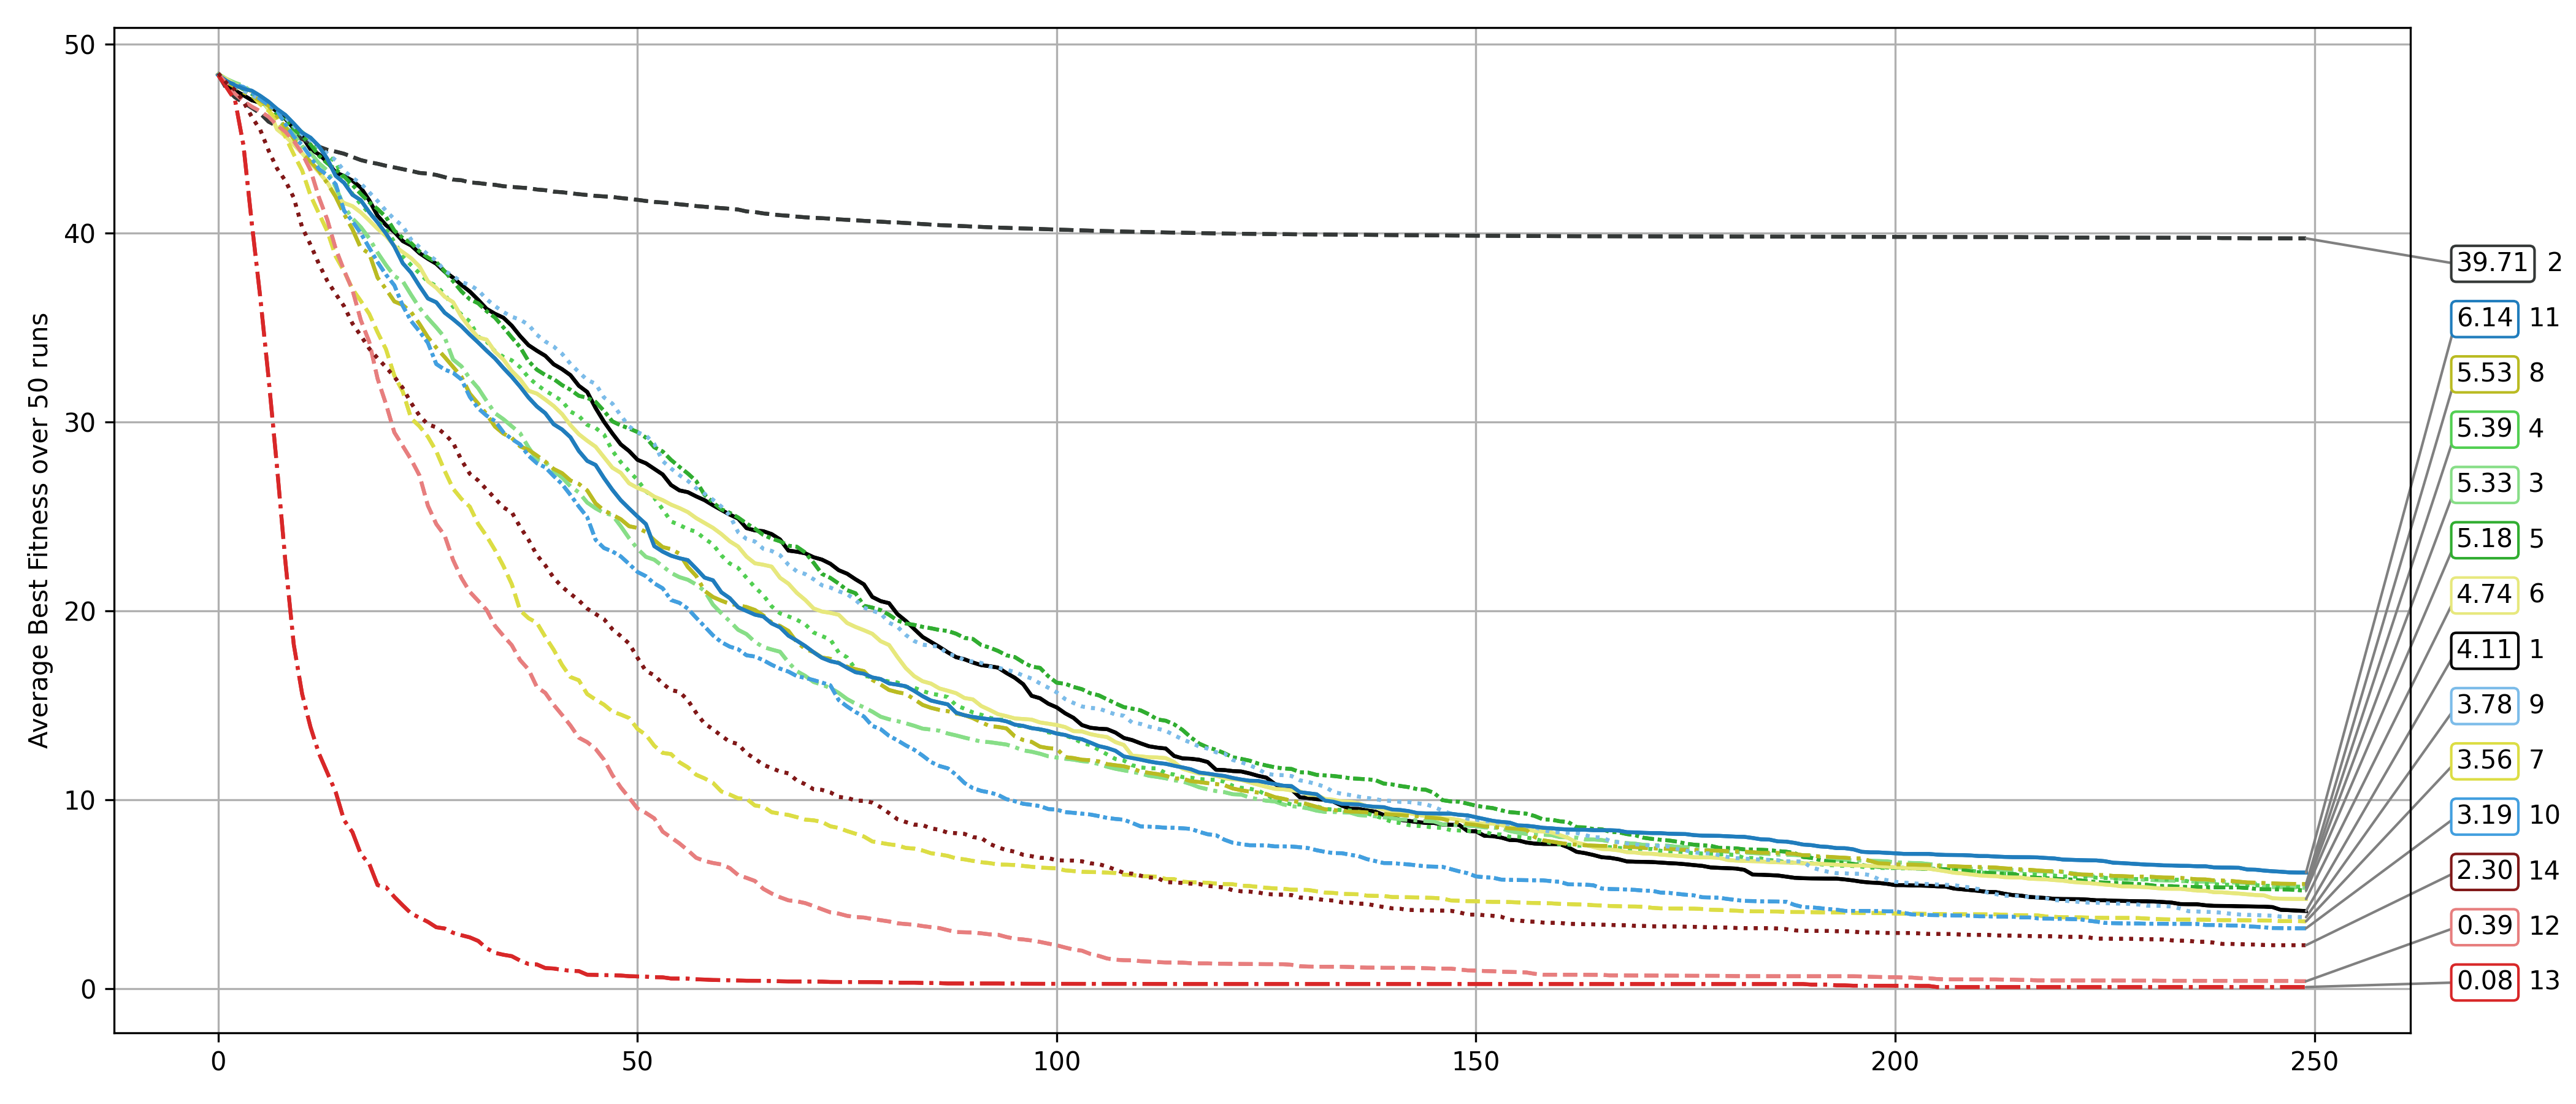
\includegraphics[width=.49\textwidth]{Figures/results/100/Generalized_Schaffer_N4_All_selected_algorithms_dim100_annot_legend.png}
    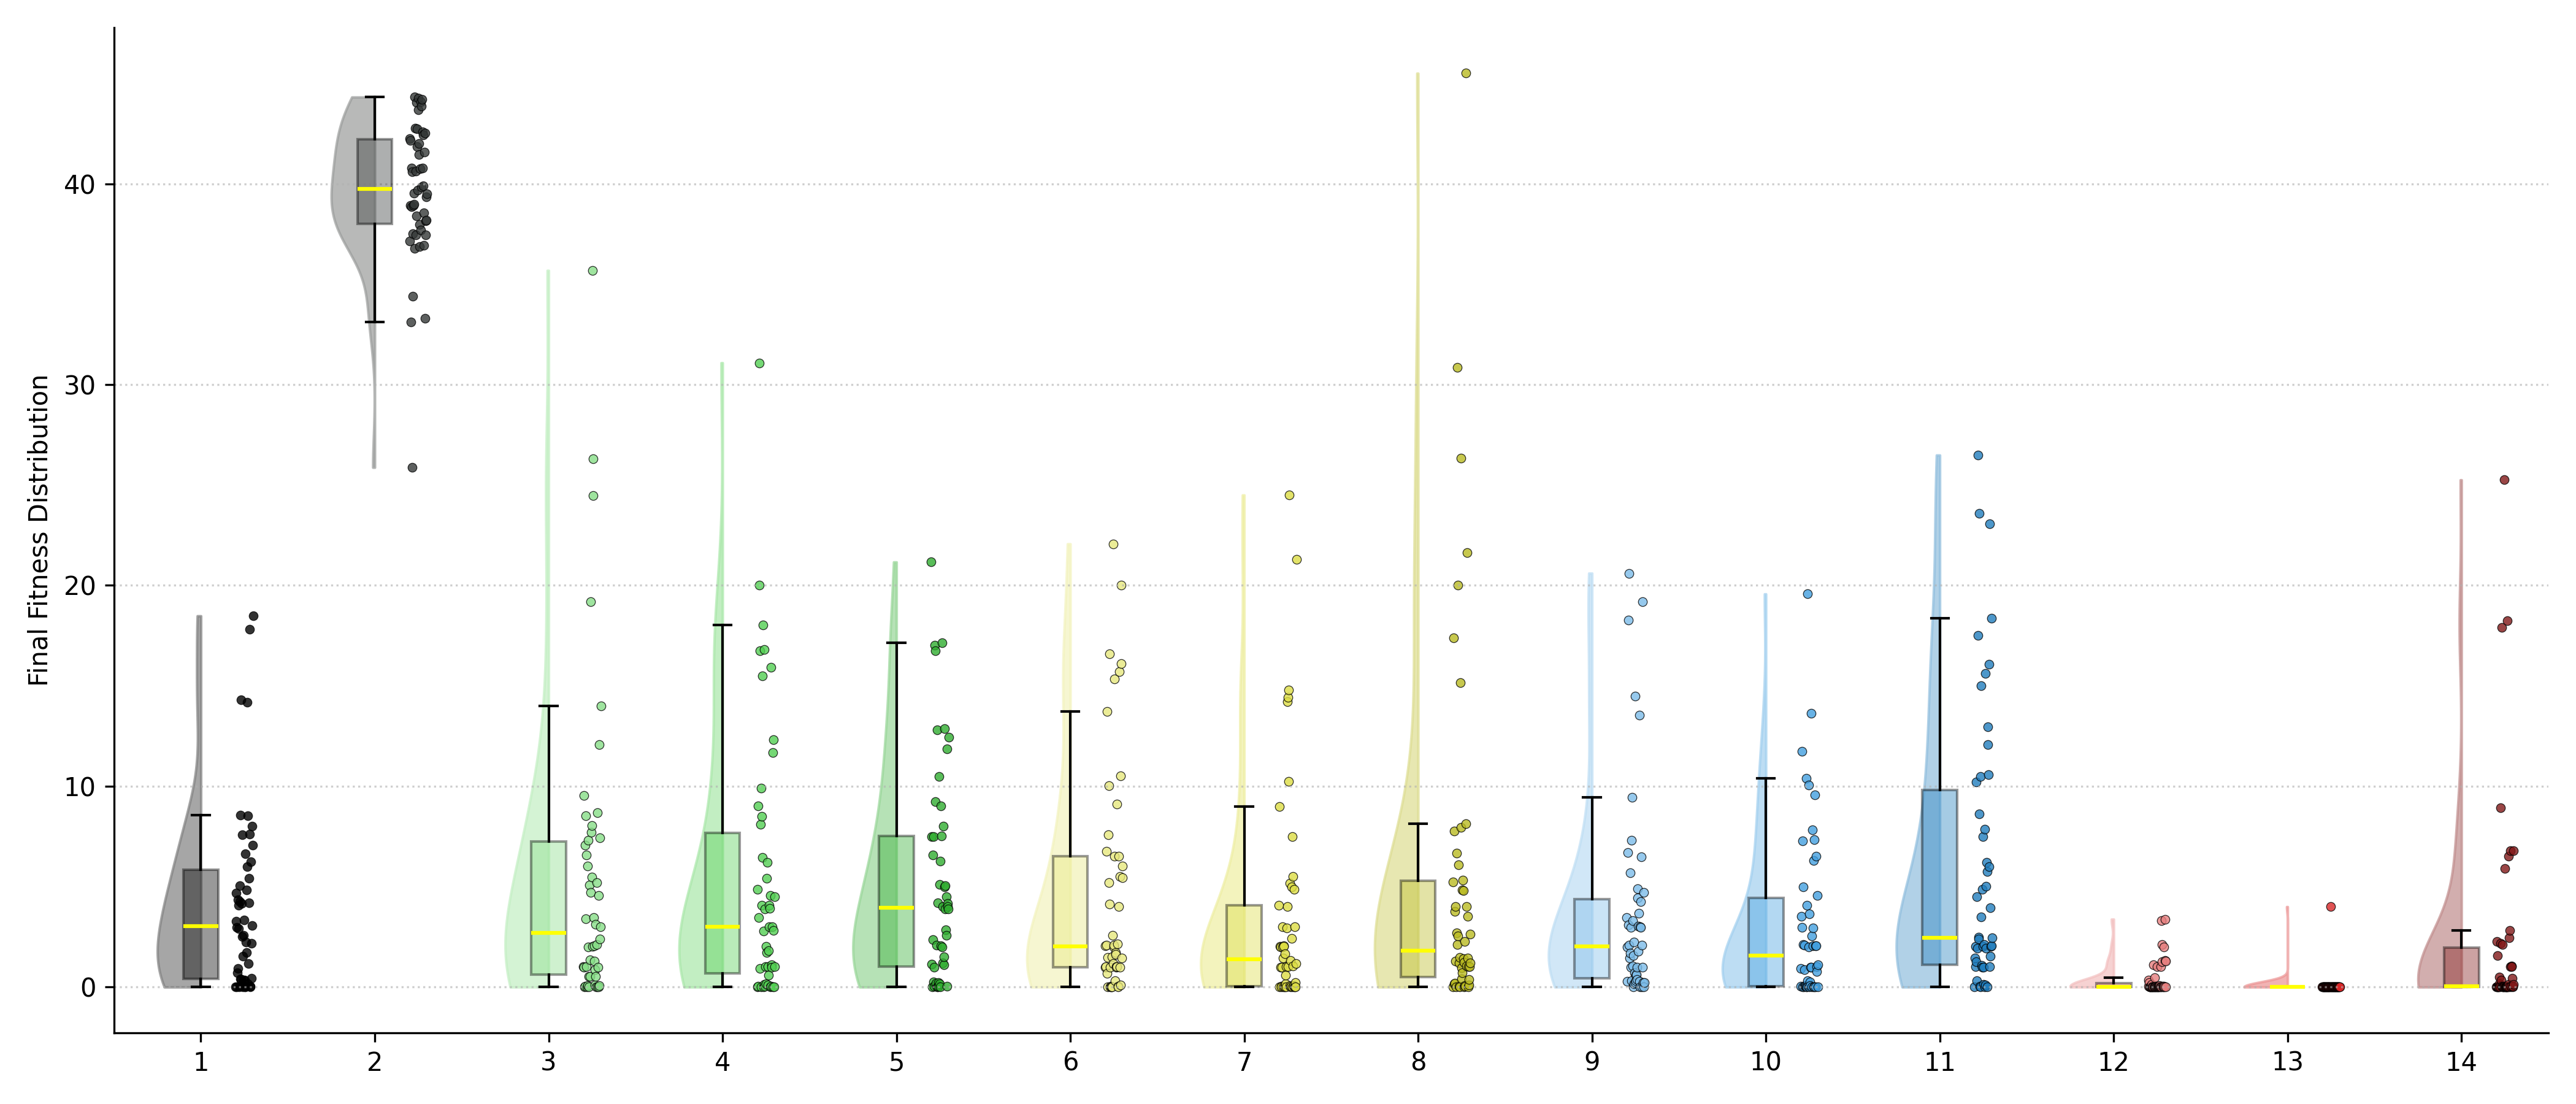
\includegraphics[width=.49\textwidth]{Figures/results/100/Generalized_Schaffer_N4_all_dim100_raincloud_vertical.png}
    \caption{Generalized Schaffer N4}
\end{subfigure}

\begin{subfigure}{1\textwidth}
    \centering
    \includegraphics[width=.49\textwidth]{Figures/results/100/Generalized_Schmidt–Vetters_All_selected_algorithms_dim100_annot_legend.png}
    \includegraphics[width=.49\textwidth]{Figures/results/100/Generalized_Schmidt–Vetters_all_dim100_raincloud_vertical.png}
    \caption{Generalized Schmidt–Vetters}
\end{subfigure}

\begin{subfigure}{1\textwidth}
    \centering
    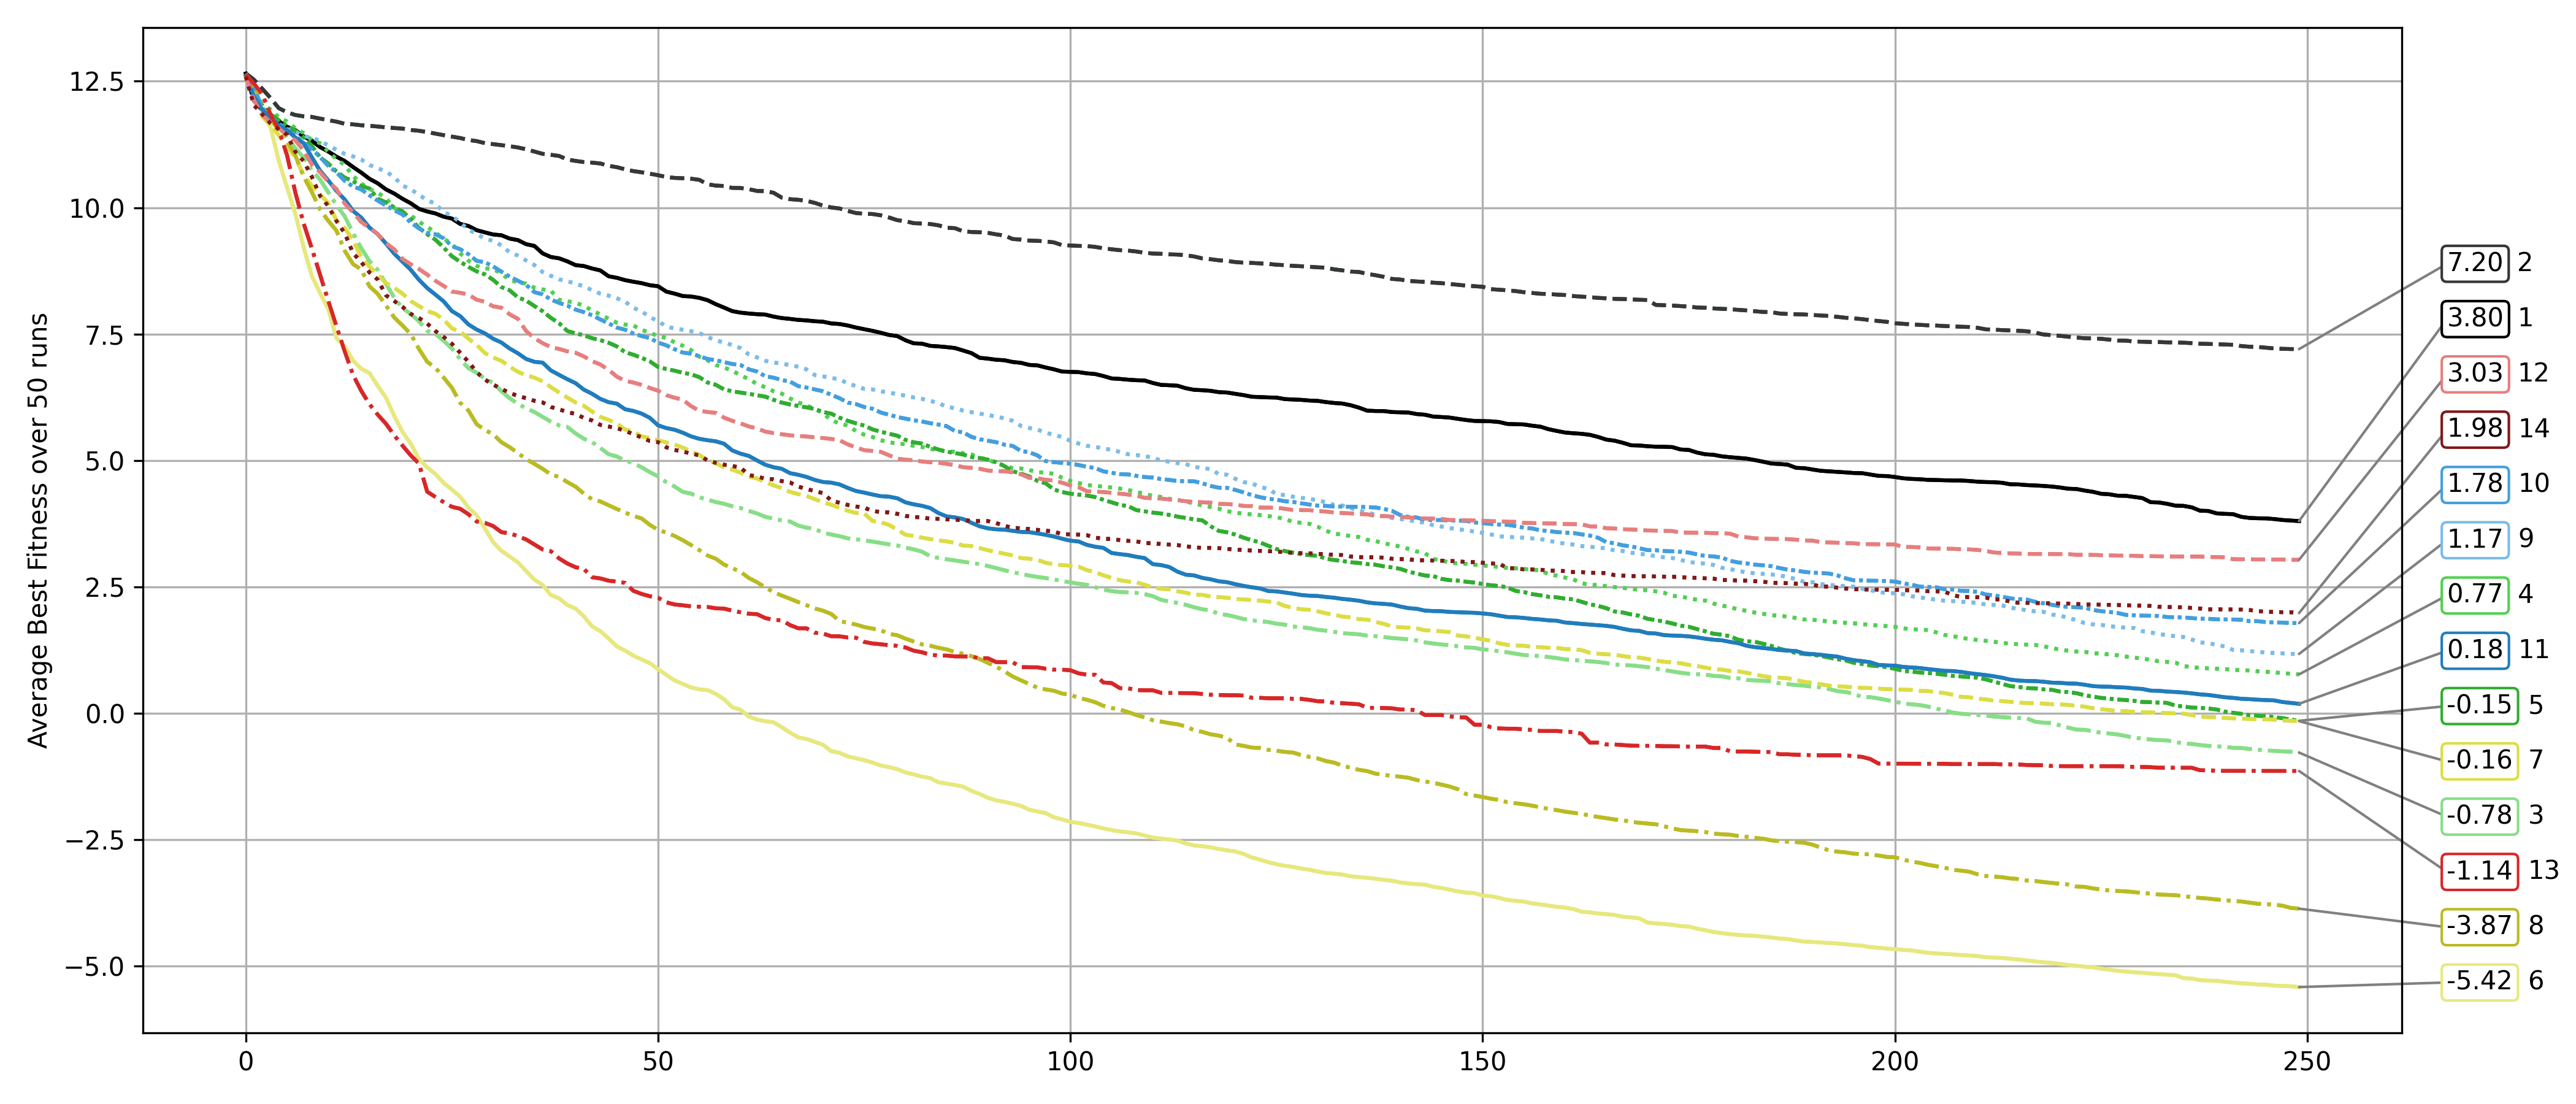
\includegraphics[width=.49\textwidth]{Figures/results/100/Lennard_Jones_Minimum_Energy_Cluster_All_selected_algorithms_dim100_annot_legend.png}
    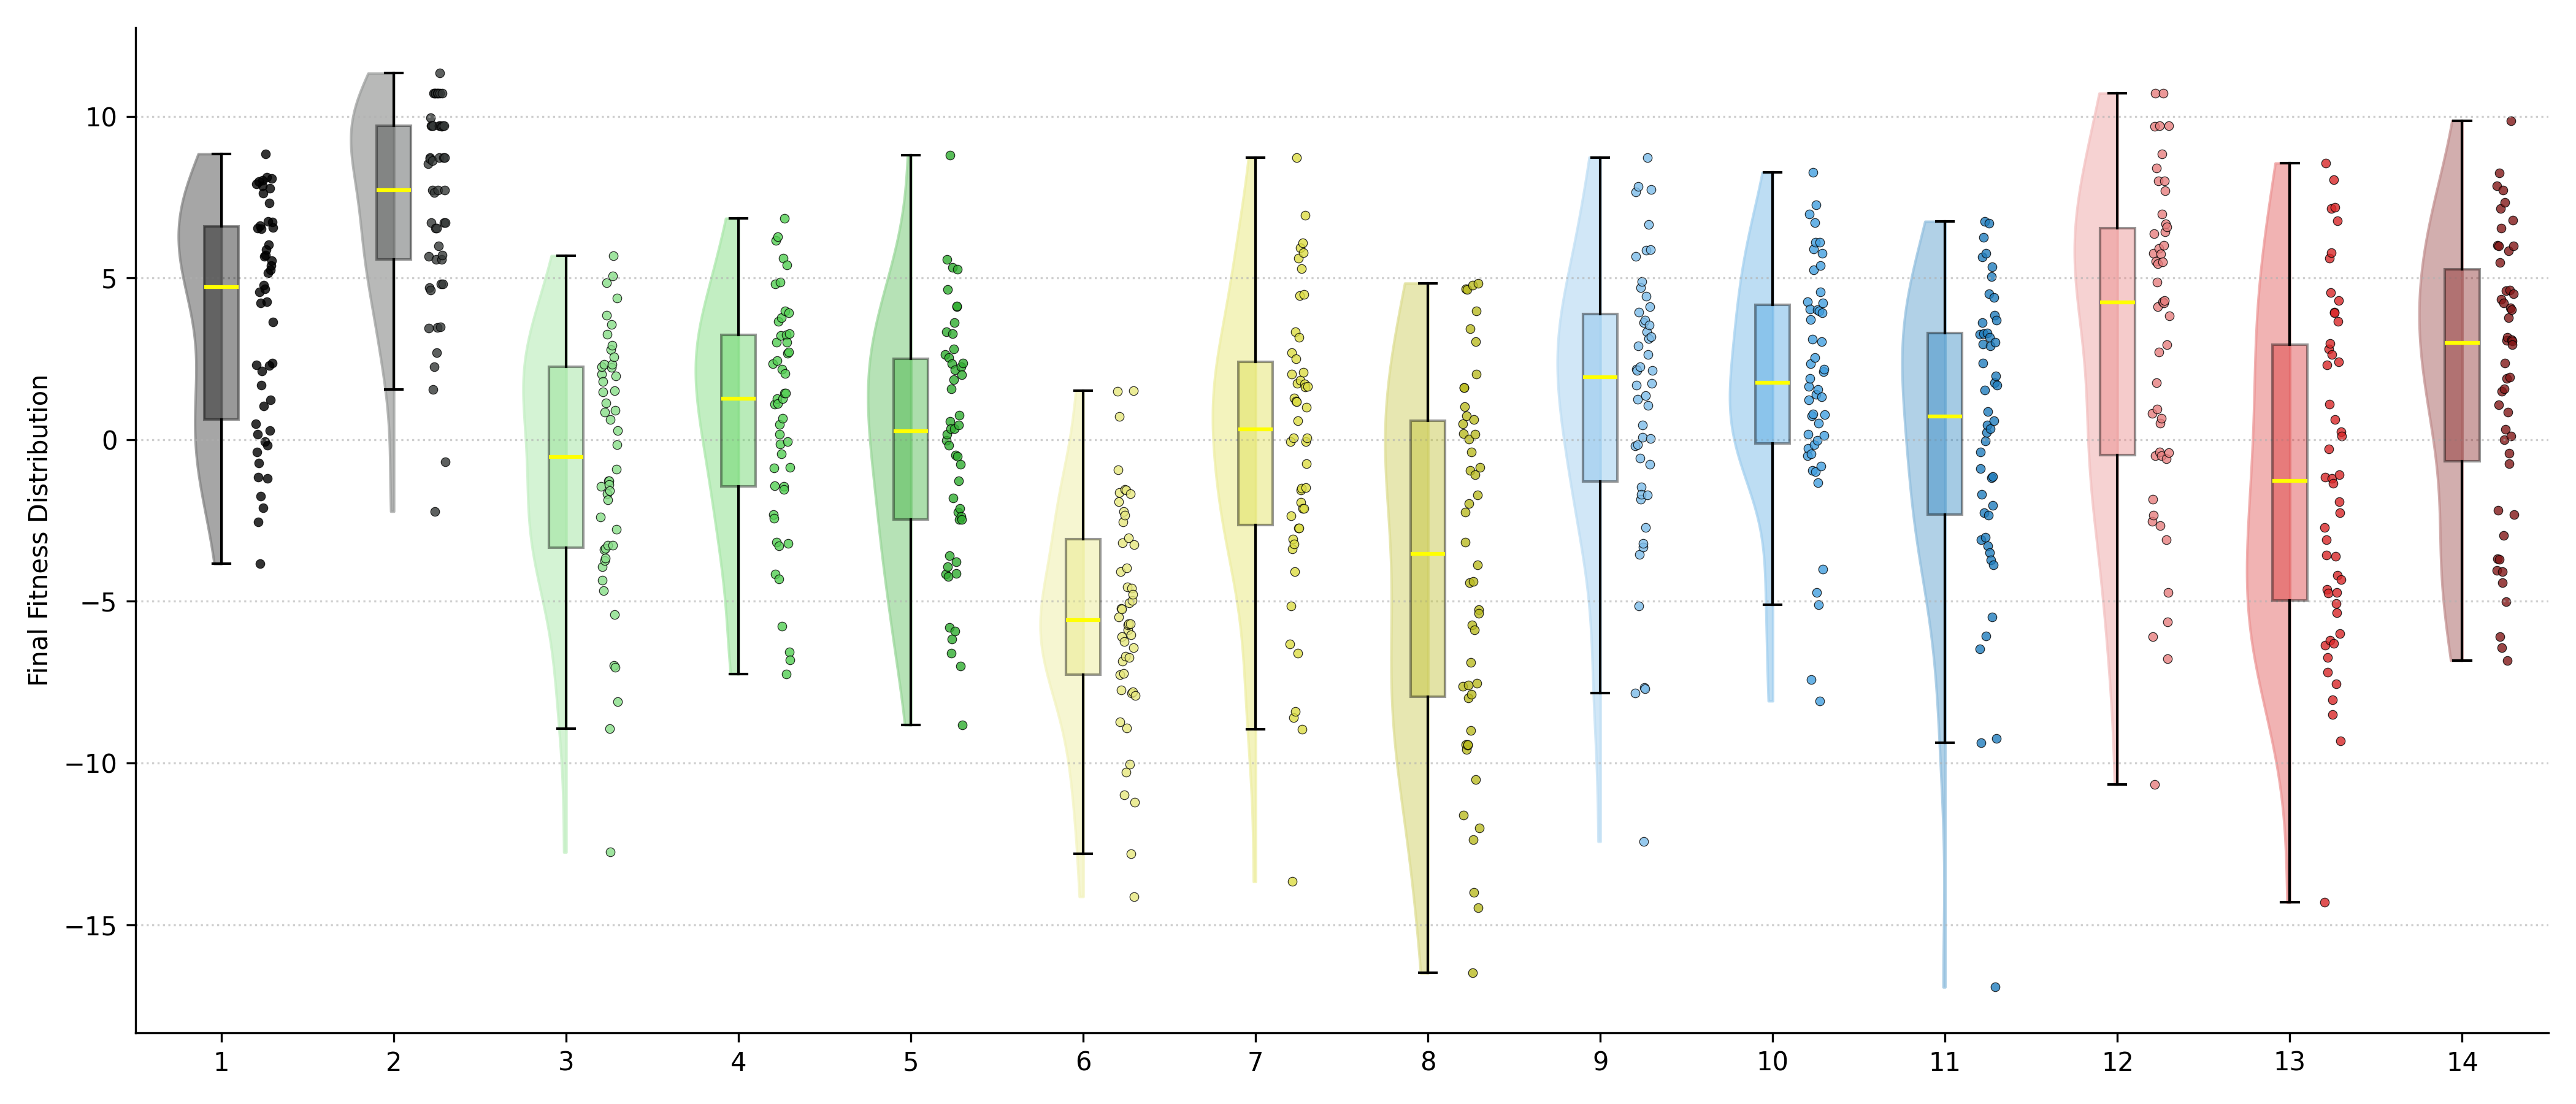
\includegraphics[width=.49\textwidth]{Figures/results/100/Lennard_Jones_Minimum_Energy_Cluster_all_dim100_raincloud_vertical.png}
    \caption{Lennard-Jones Minimum Energy Cluster}
\end{subfigure}

\begin{subfigure}{1\textwidth}
    \centering
    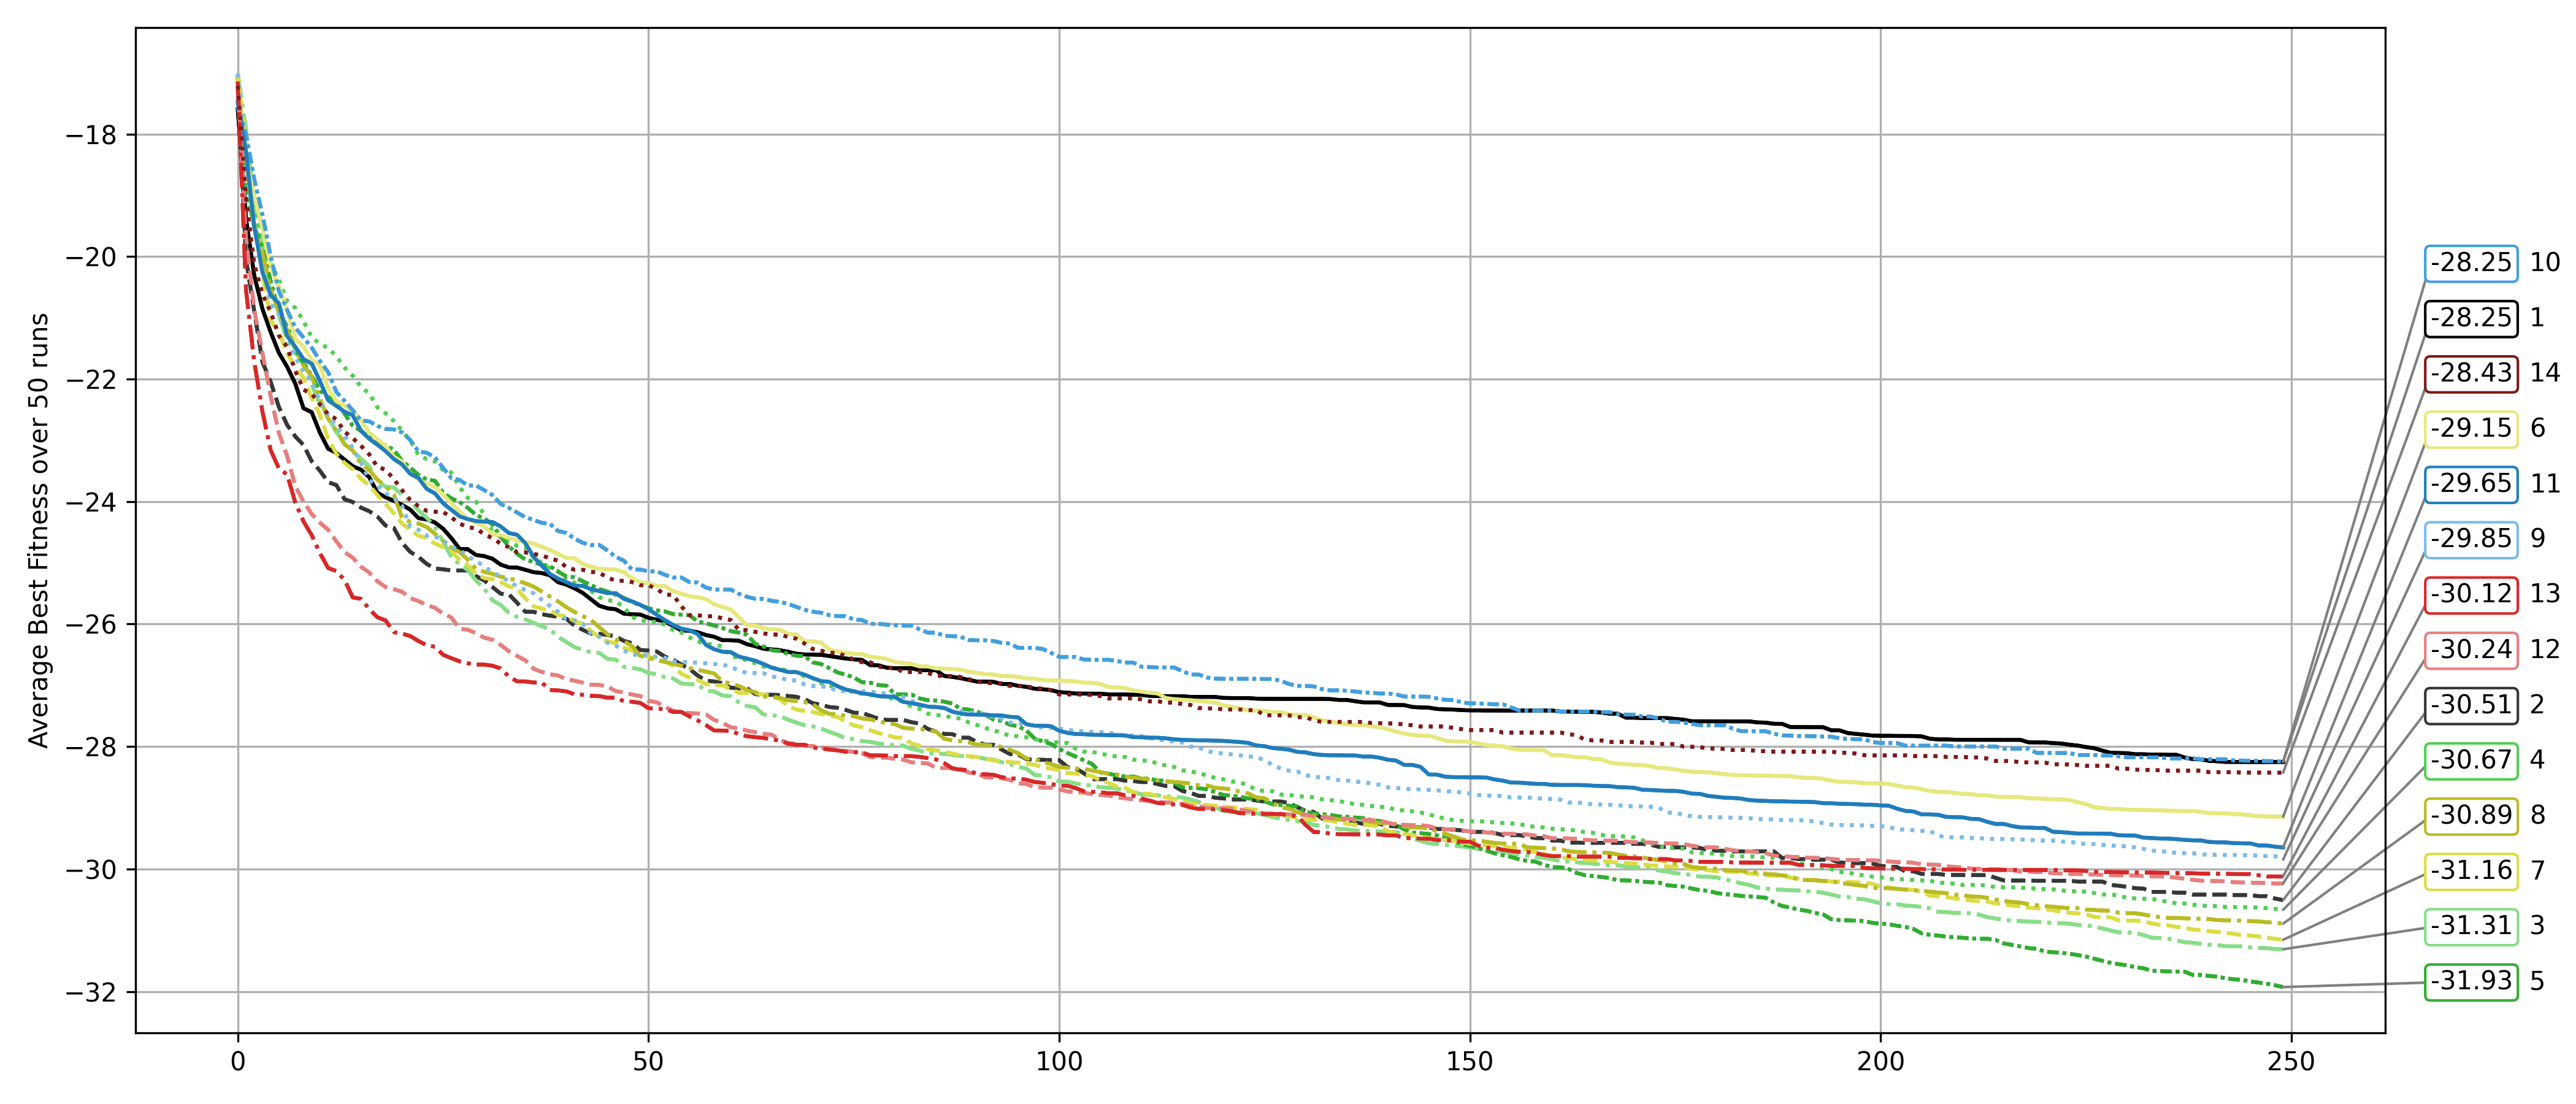
\includegraphics[width=.49\textwidth]{Figures/results/100/Michalewicz_All_selected_algorithms_dim100_annot_legend.png}
    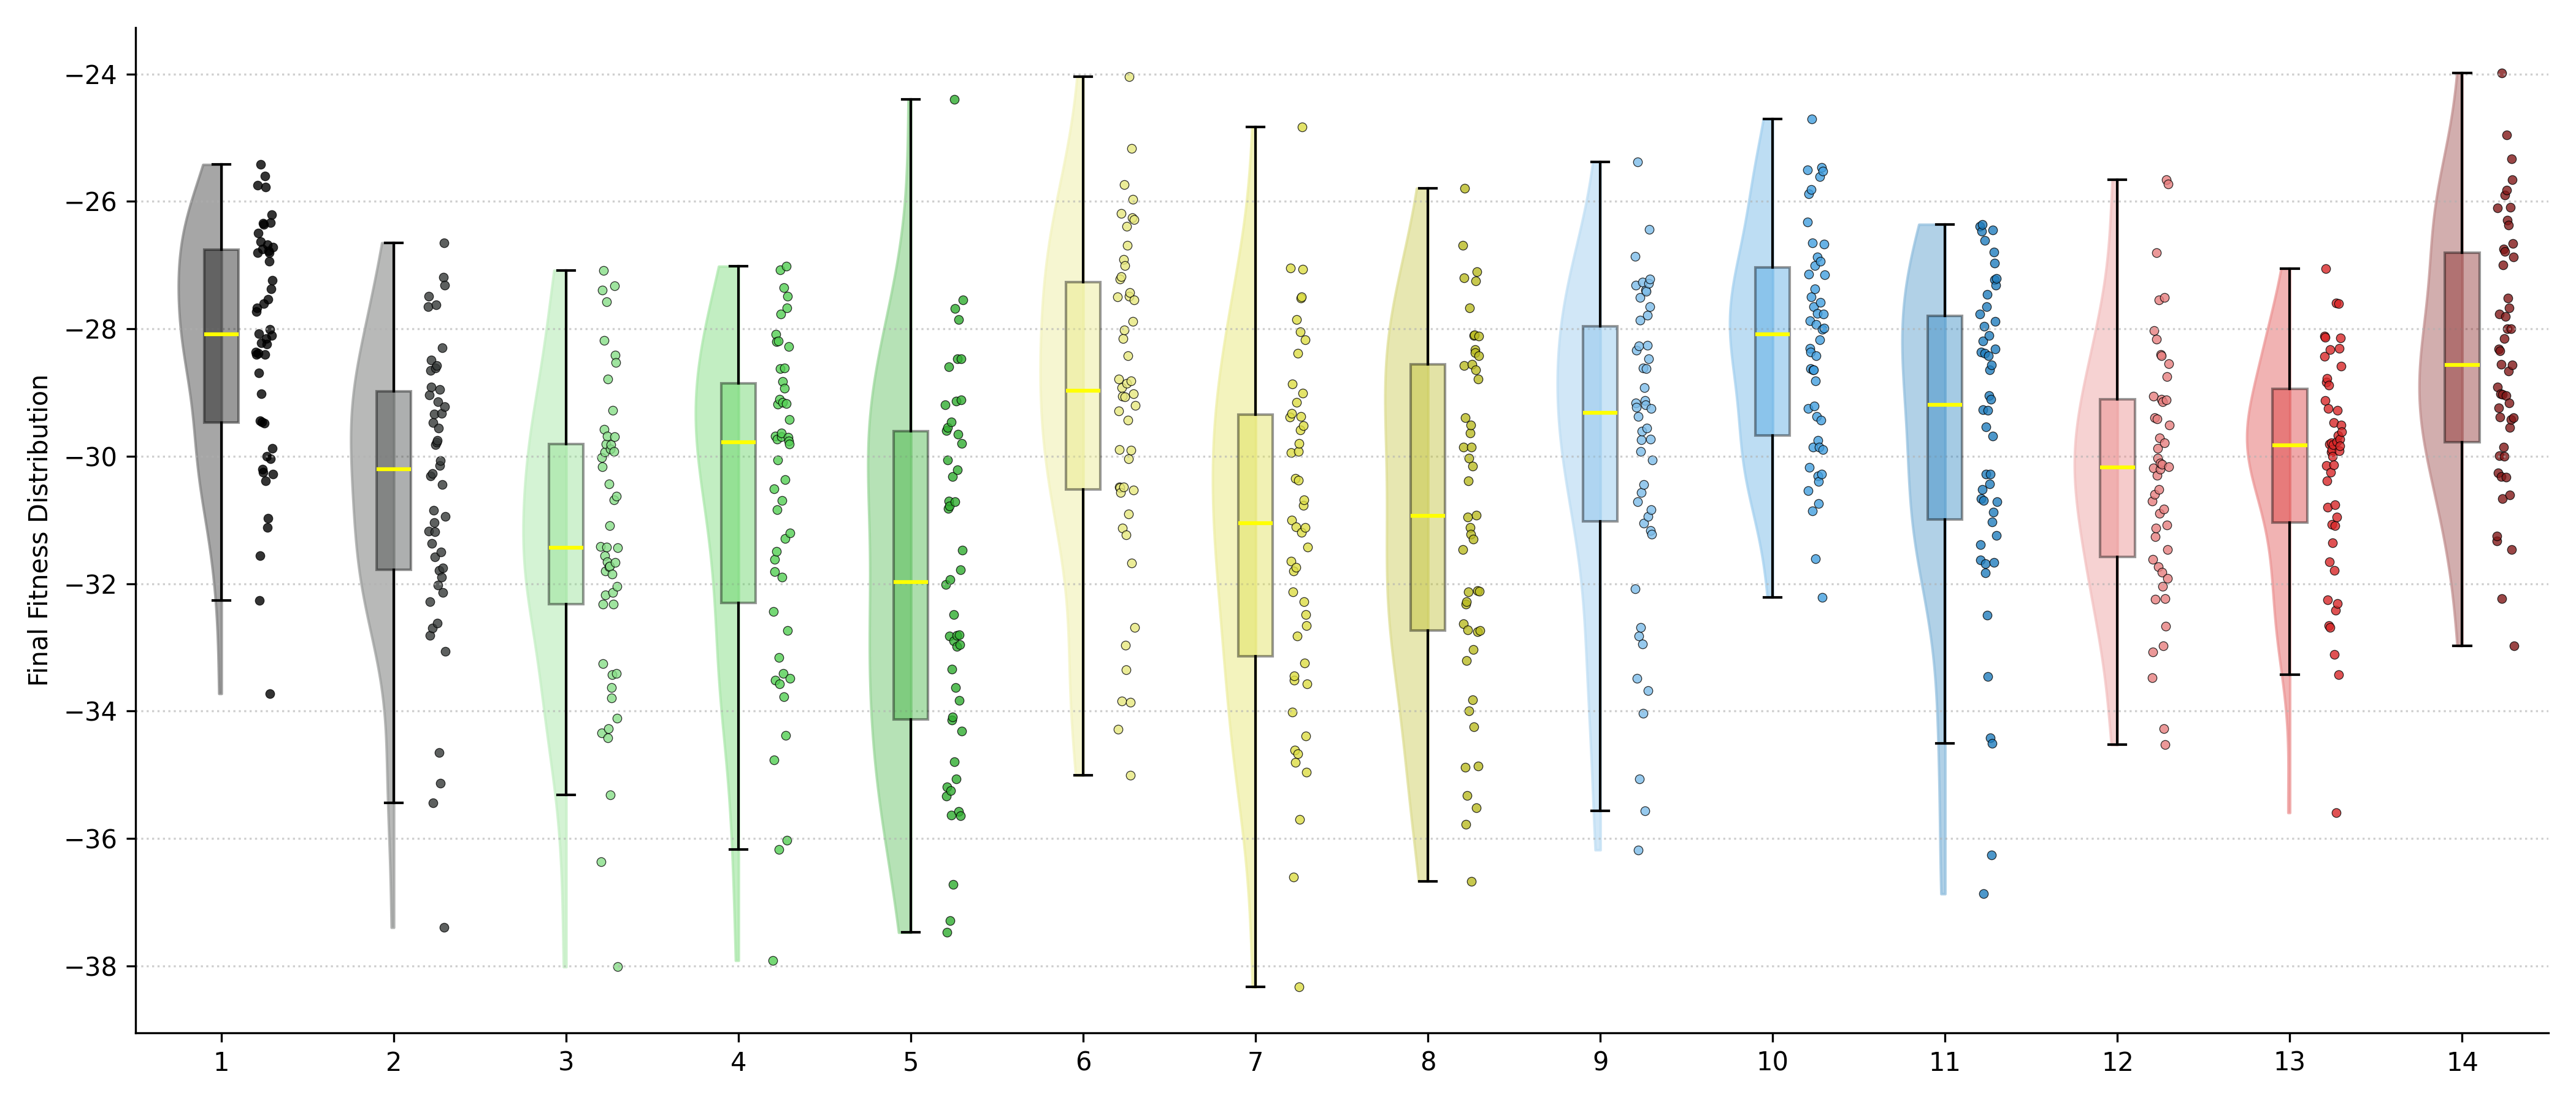
\includegraphics[width=.49\textwidth]{Figures/results/100/Michalewicz_all_dim100_raincloud_vertical.png}
    \caption{Michalewicz}
\end{subfigure}

\begin{subfigure}{1\textwidth}
    \centering
    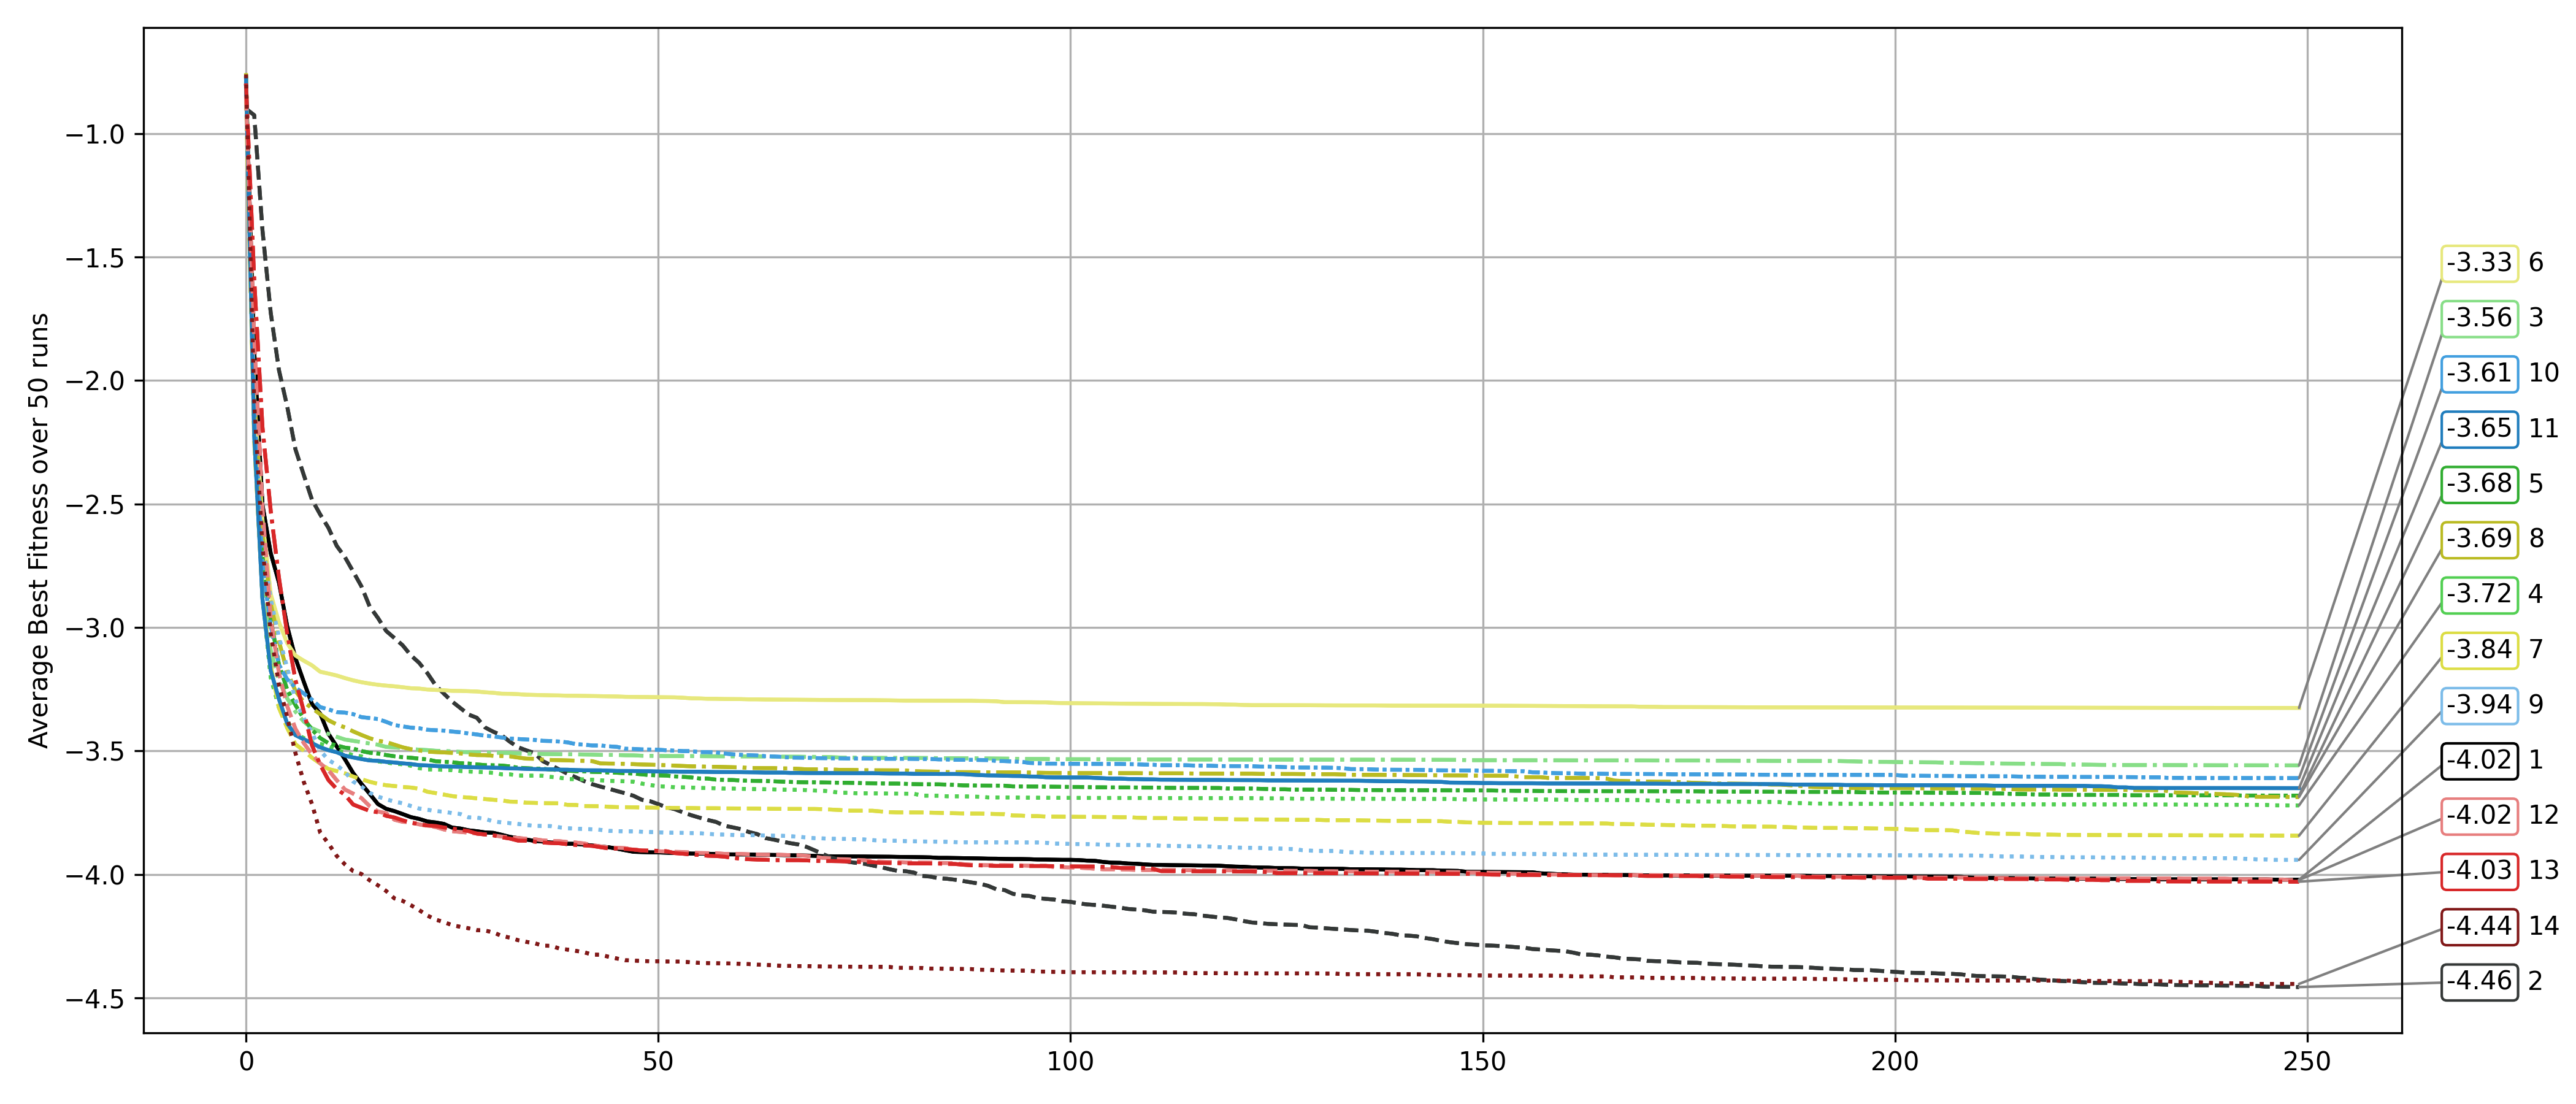
\includegraphics[width=.49\textwidth]{Figures/results/100/Mishra_N3_All_selected_algorithms_dim100_annot_legend.png}
    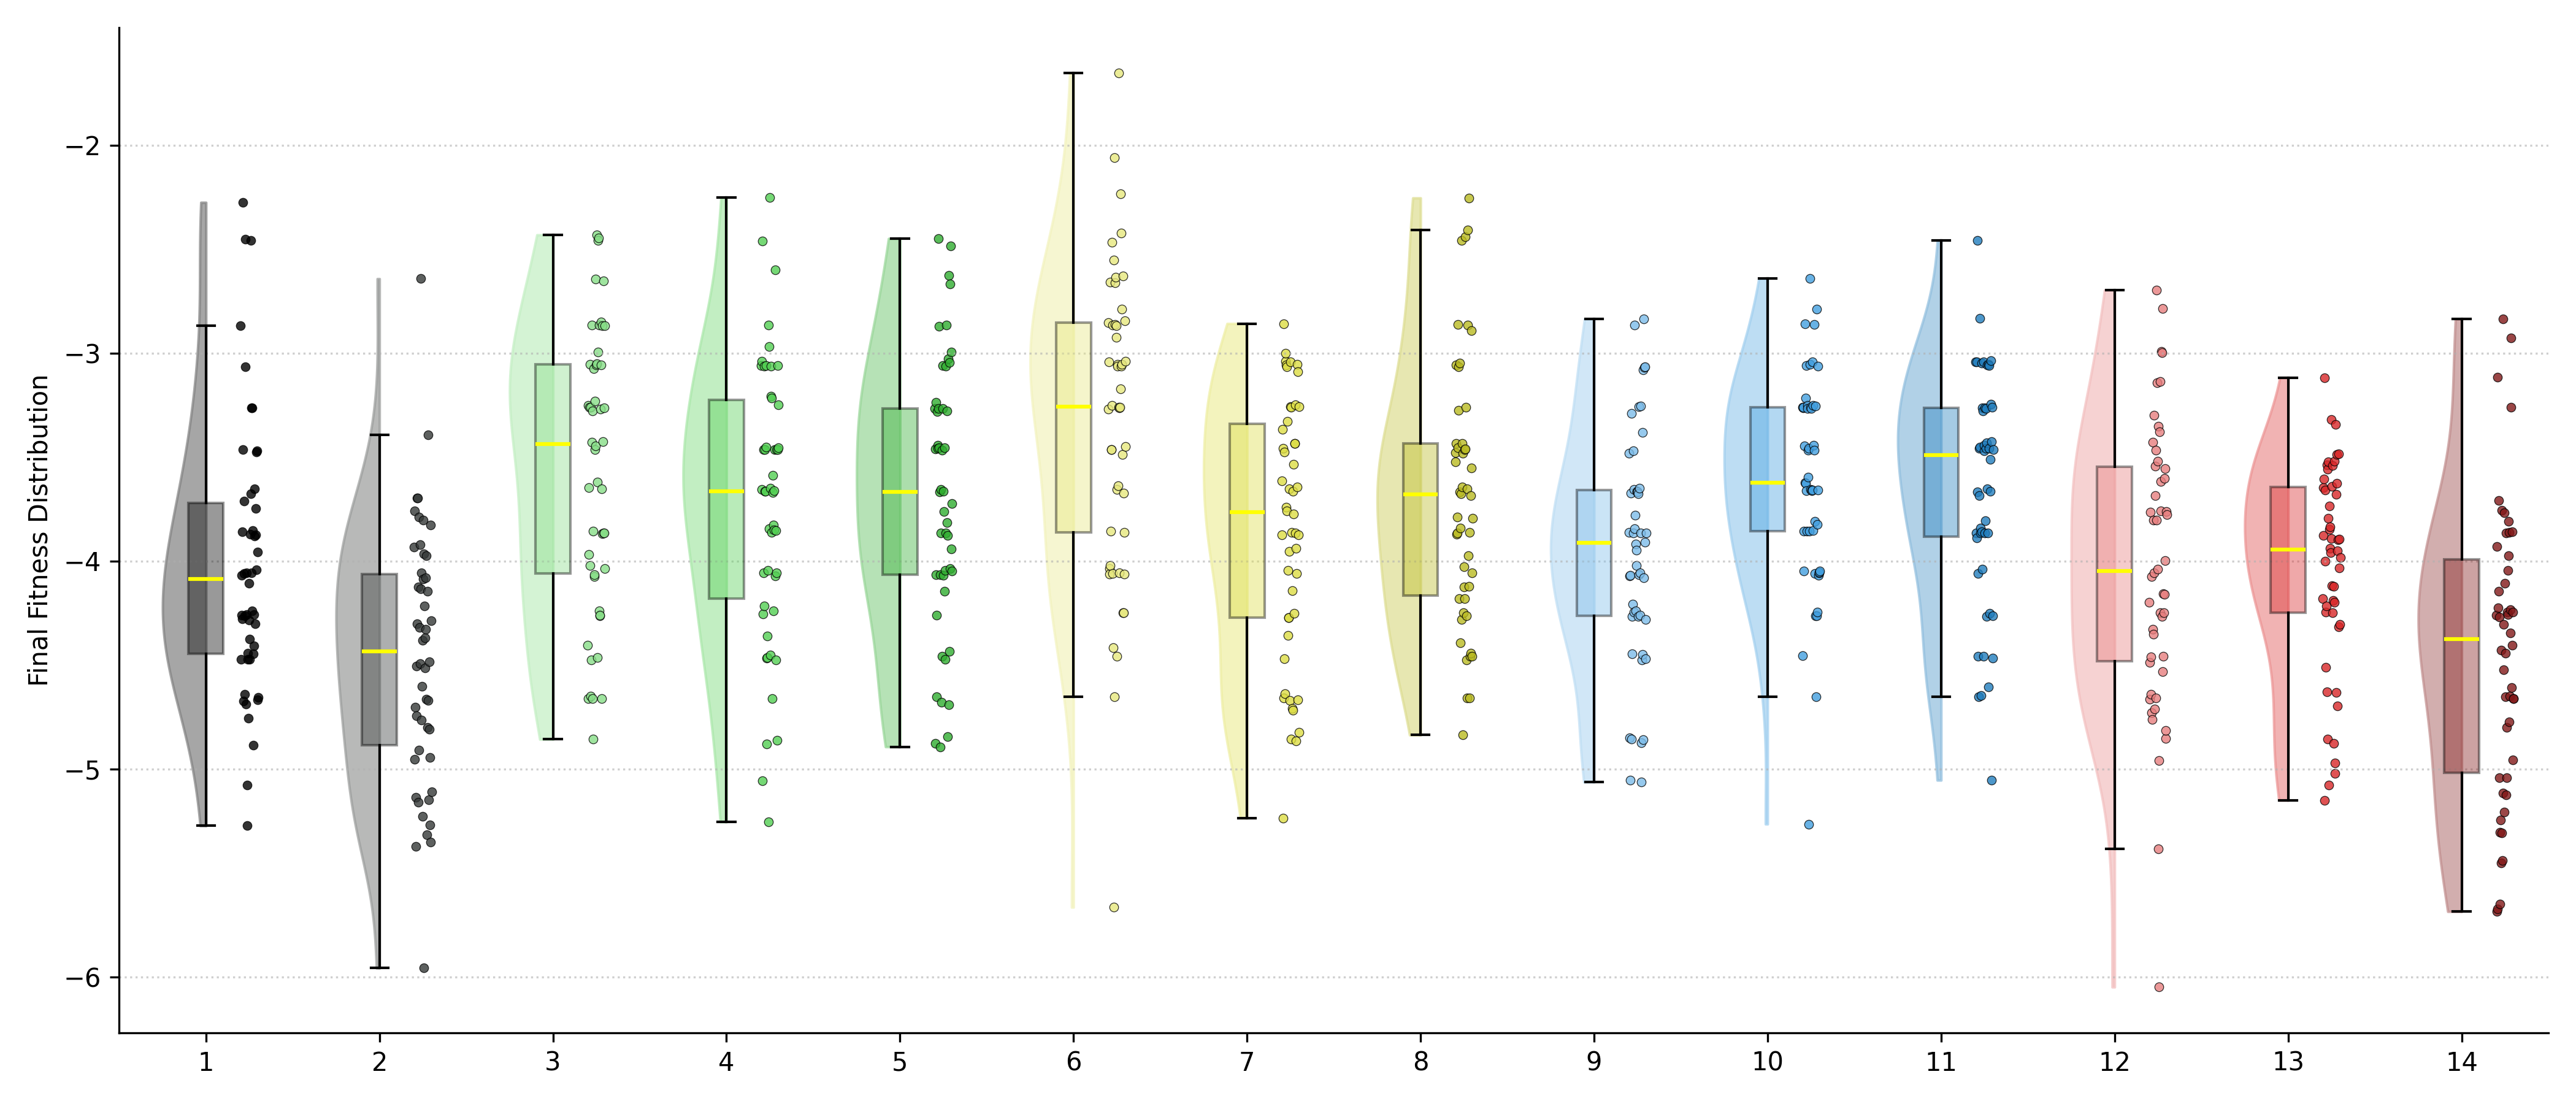
\includegraphics[width=.49\textwidth]{Figures/results/100/Mishra_N3_all_dim100_raincloud_vertical.png}
    \caption{Mishra N3}
\end{subfigure}


\captionsetup{list=no}
\caption[Convergence curves and final fitness distribution raincloud plots for 100-dimensional problems]{Convergence curves (left) and final fitness distribution raincloud plots (right) for each tested benchmark problem in the 100-dimensional setting. Algorithms are numbered, line-styled, ordered, and color-coded consistently according to the legend in Figure~\ref{fig:plot_encoding}. Problems plotted on a logarithmic scale are indicated with ``(log)'' following the problem name.}
\end{figure}




%%%%%%%%%%%%%%%%%%%%%%%%%%%



\begin{figure}[p]\ContinuedFloat
\renewcommand\thesubfigure{C.\arabic{figure}.\arabic{subfigure}} % Local change starts here

    \centering

\begin{subfigure}{1\textwidth}
    \centering
    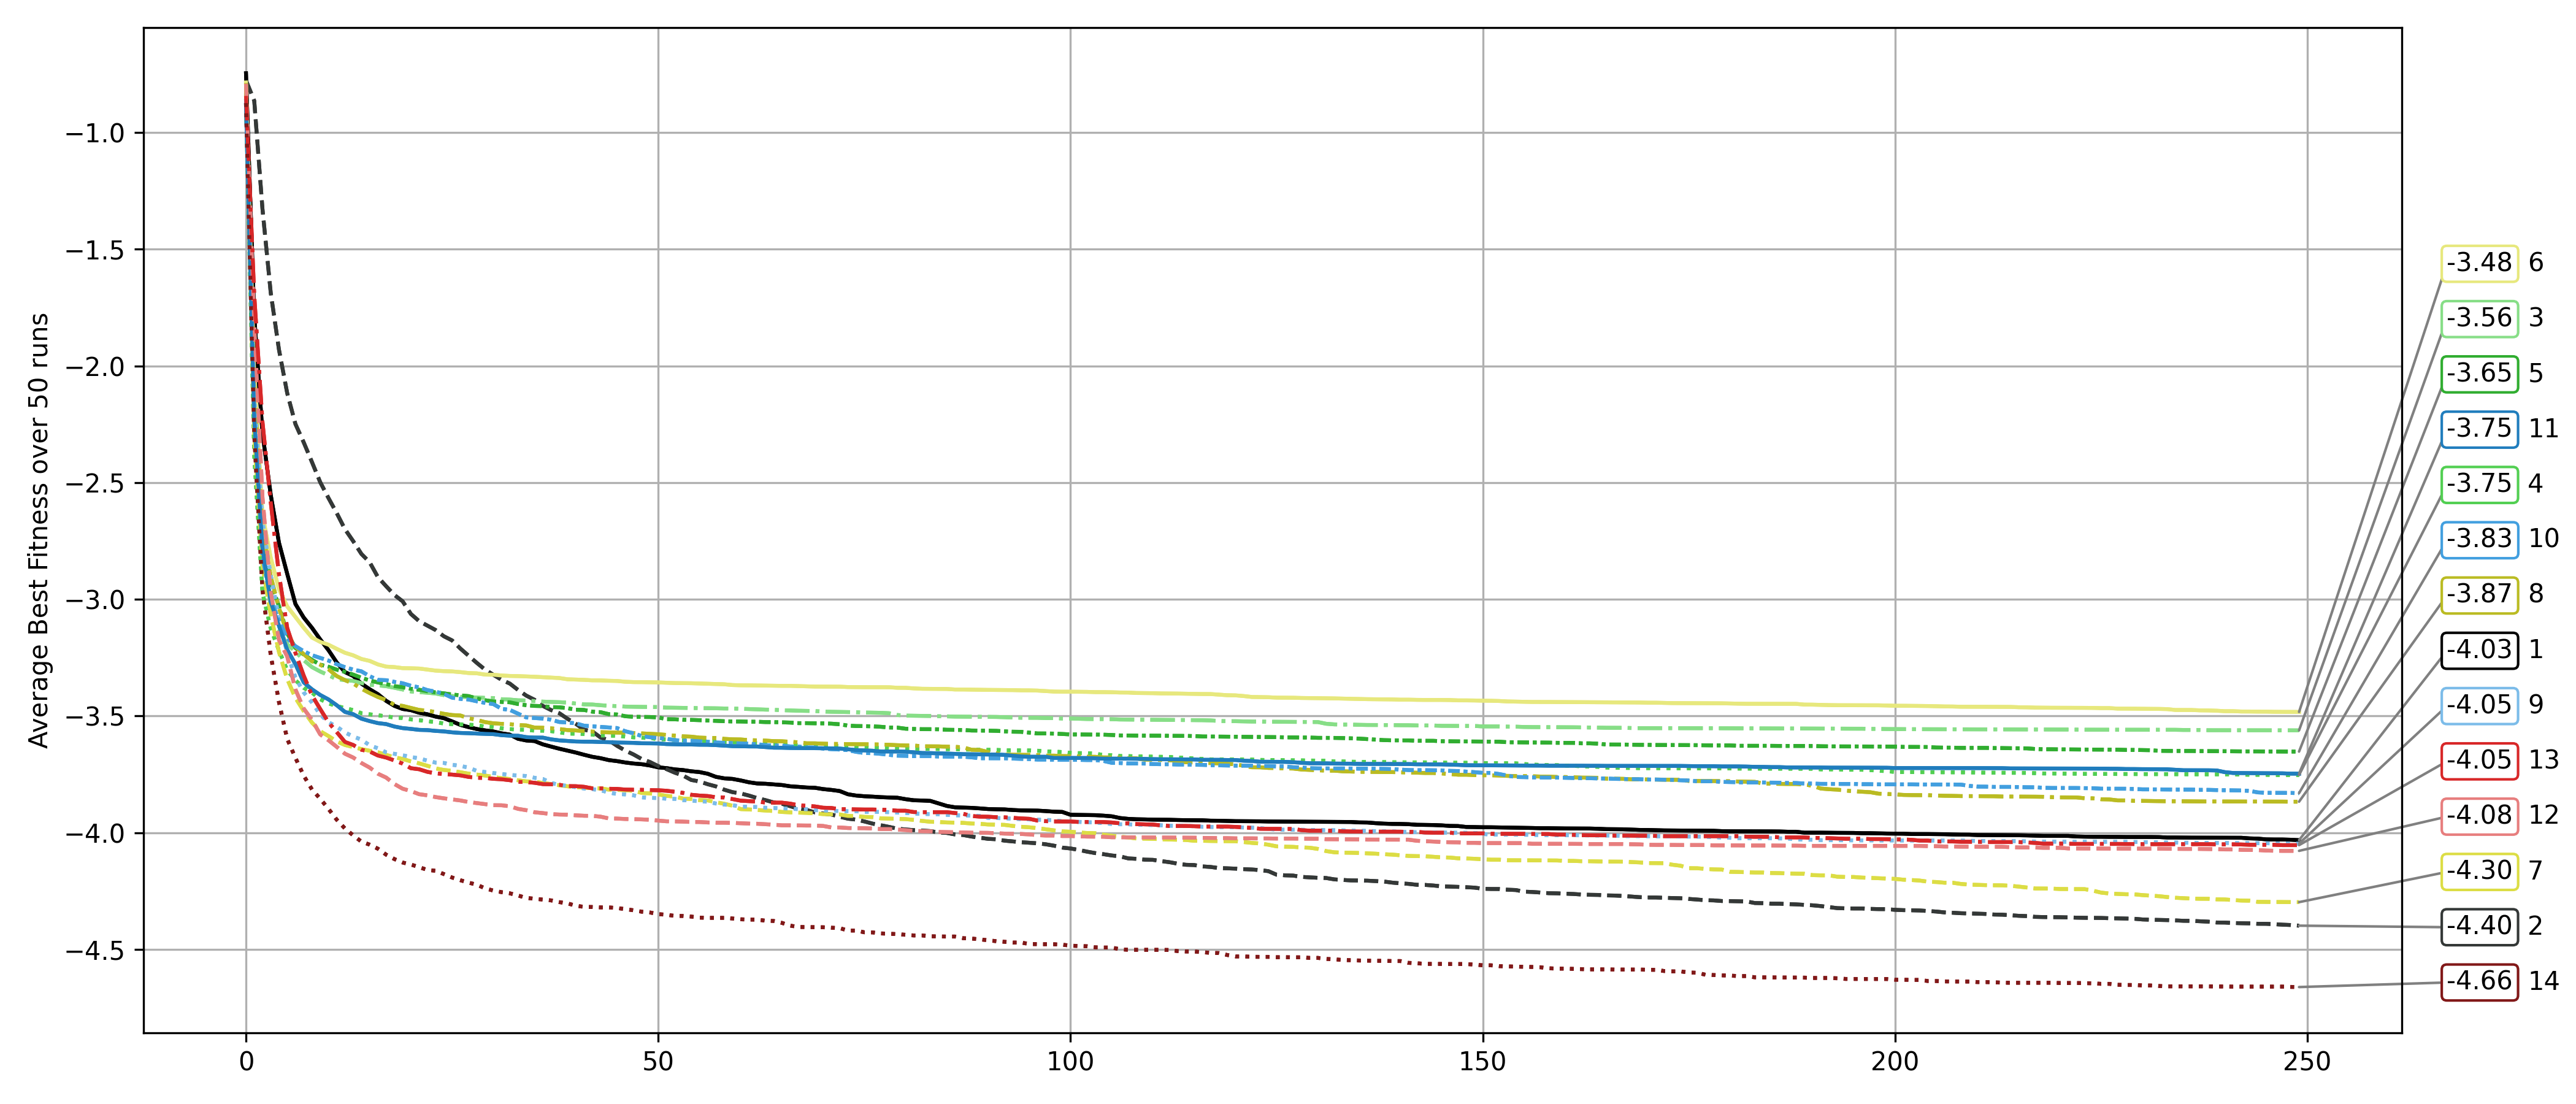
\includegraphics[width=.49\textwidth]{Figures/results/100/Mishra_N4_All_selected_algorithms_dim100_annot_legend.png}
    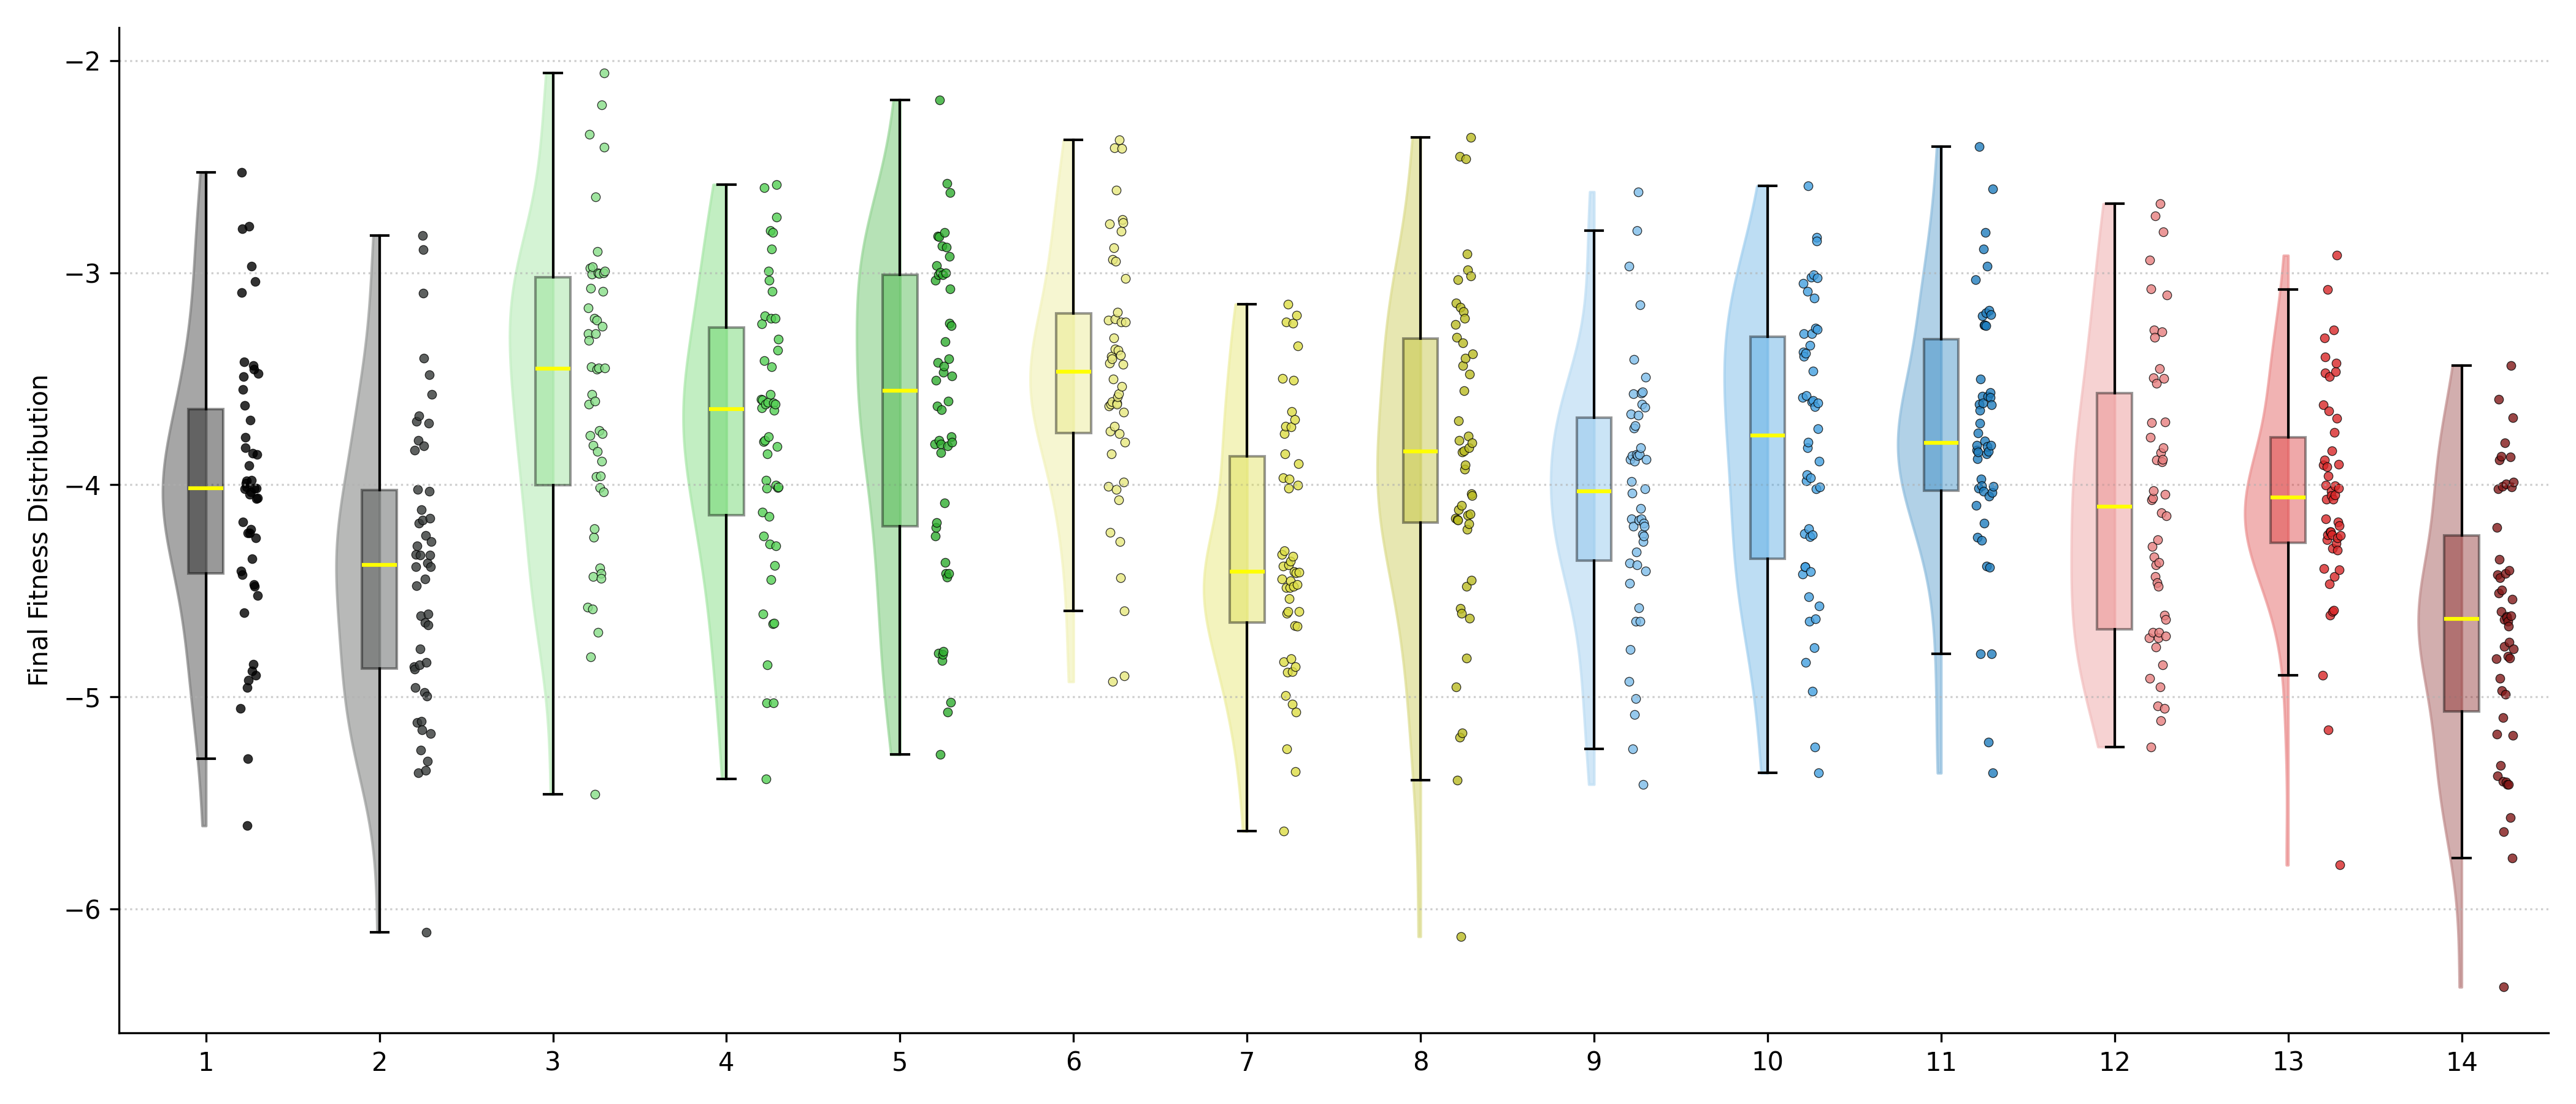
\includegraphics[width=.49\textwidth]{Figures/results/100/Mishra_N4_all_dim100_raincloud_vertical.png}
    \caption{Mishra N4}
\end{subfigure}

\begin{subfigure}{1\textwidth}
    \centering
    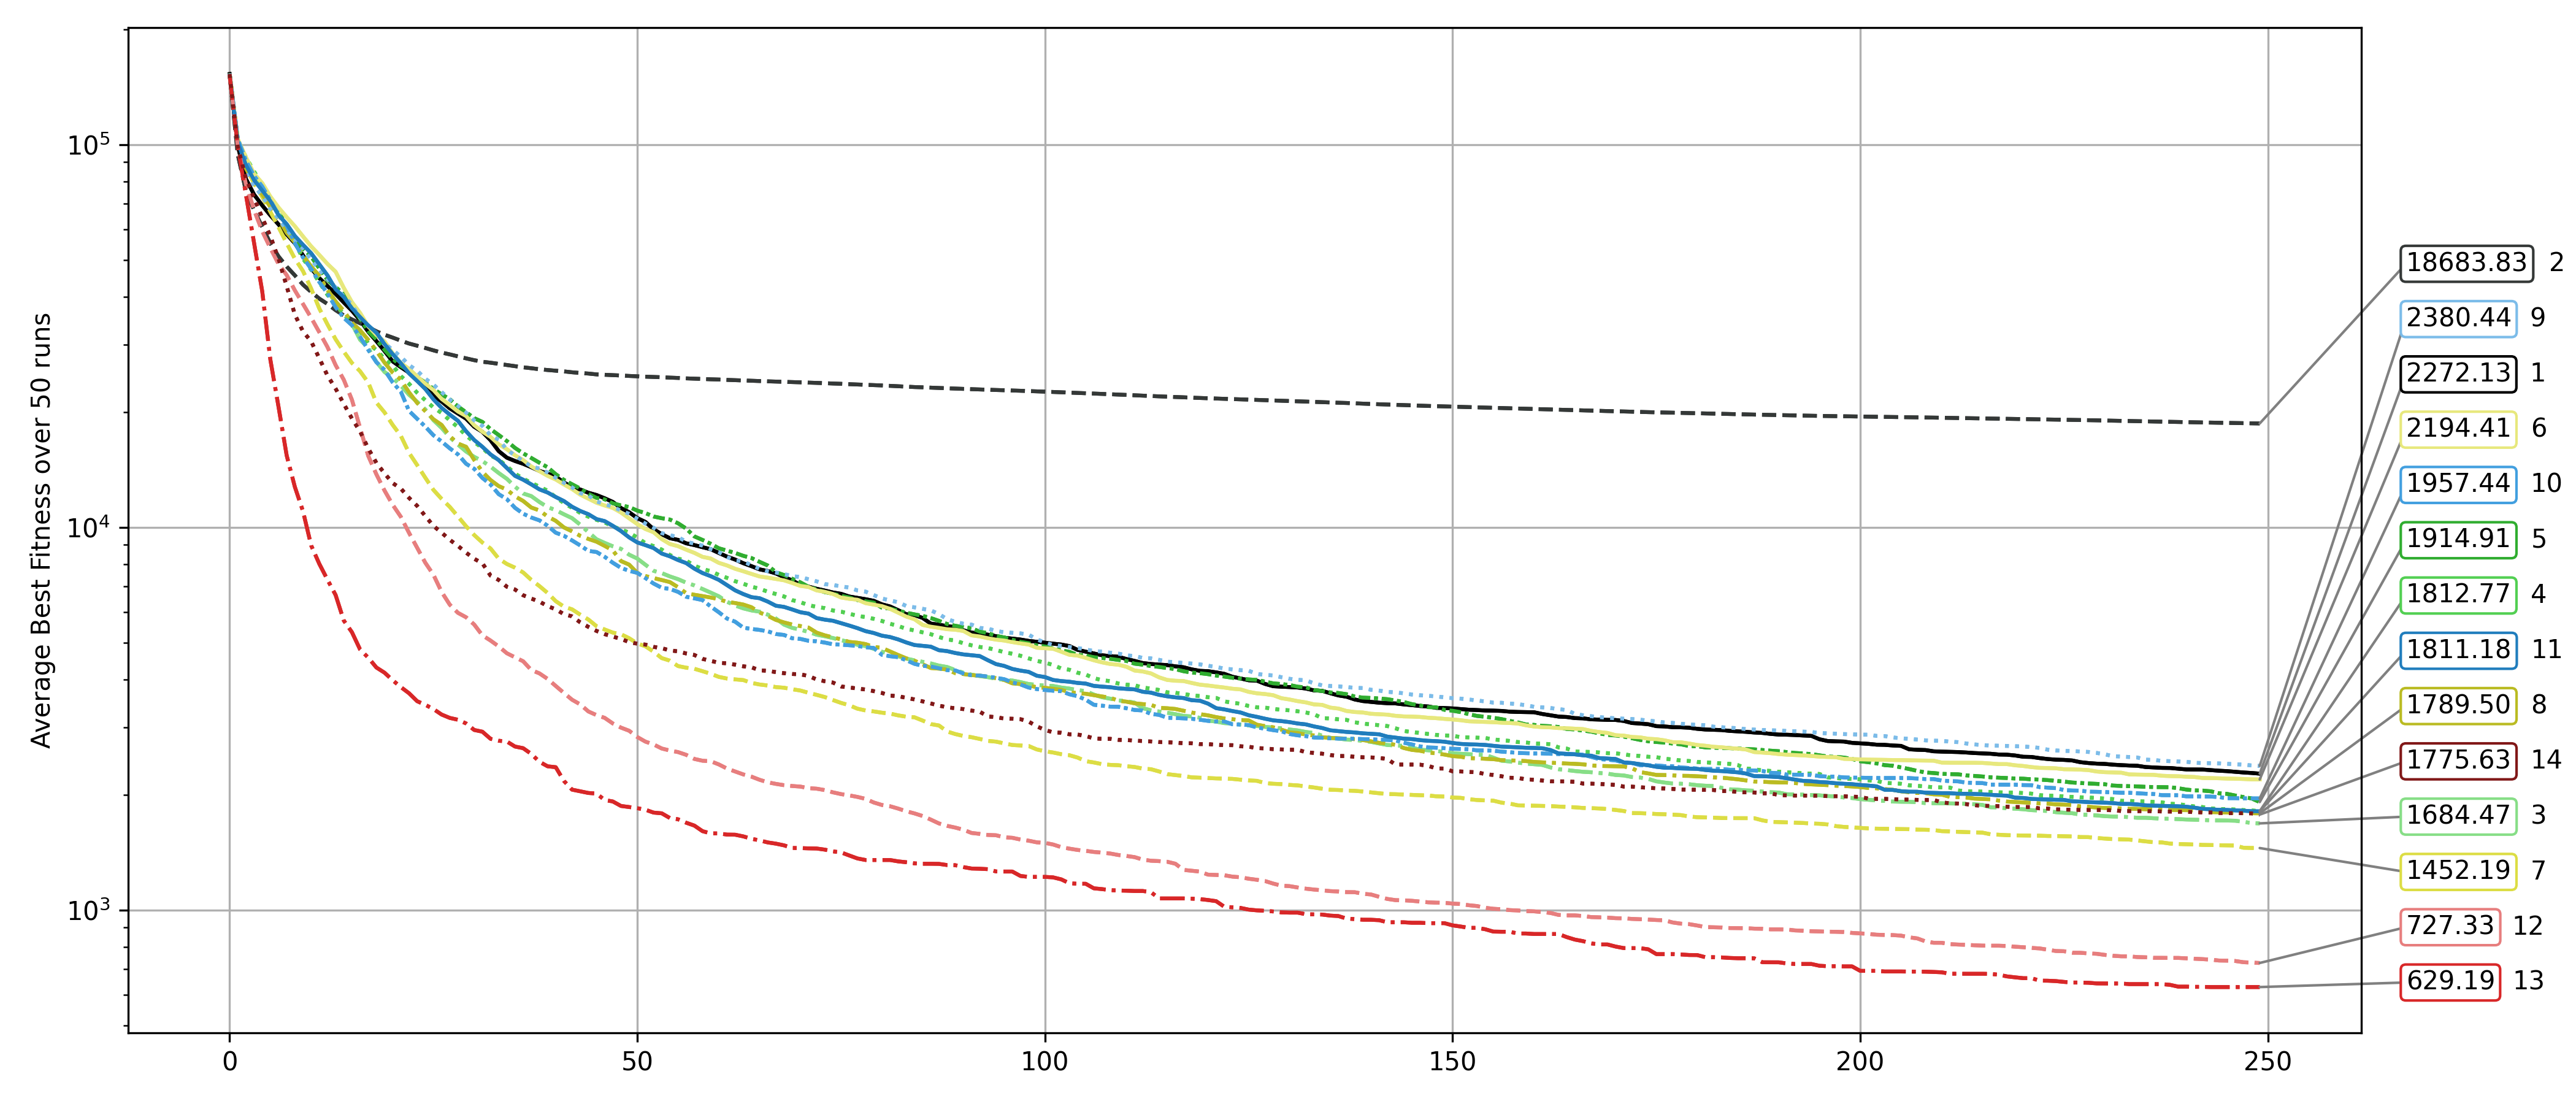
\includegraphics[width=.49\textwidth]{Figures/results/100/Modified_Rosenbrock_No.02___Hollow_Ground_Bent_Knife_Edge_All_selected_algorithms_dim100_annot_legend.png}
    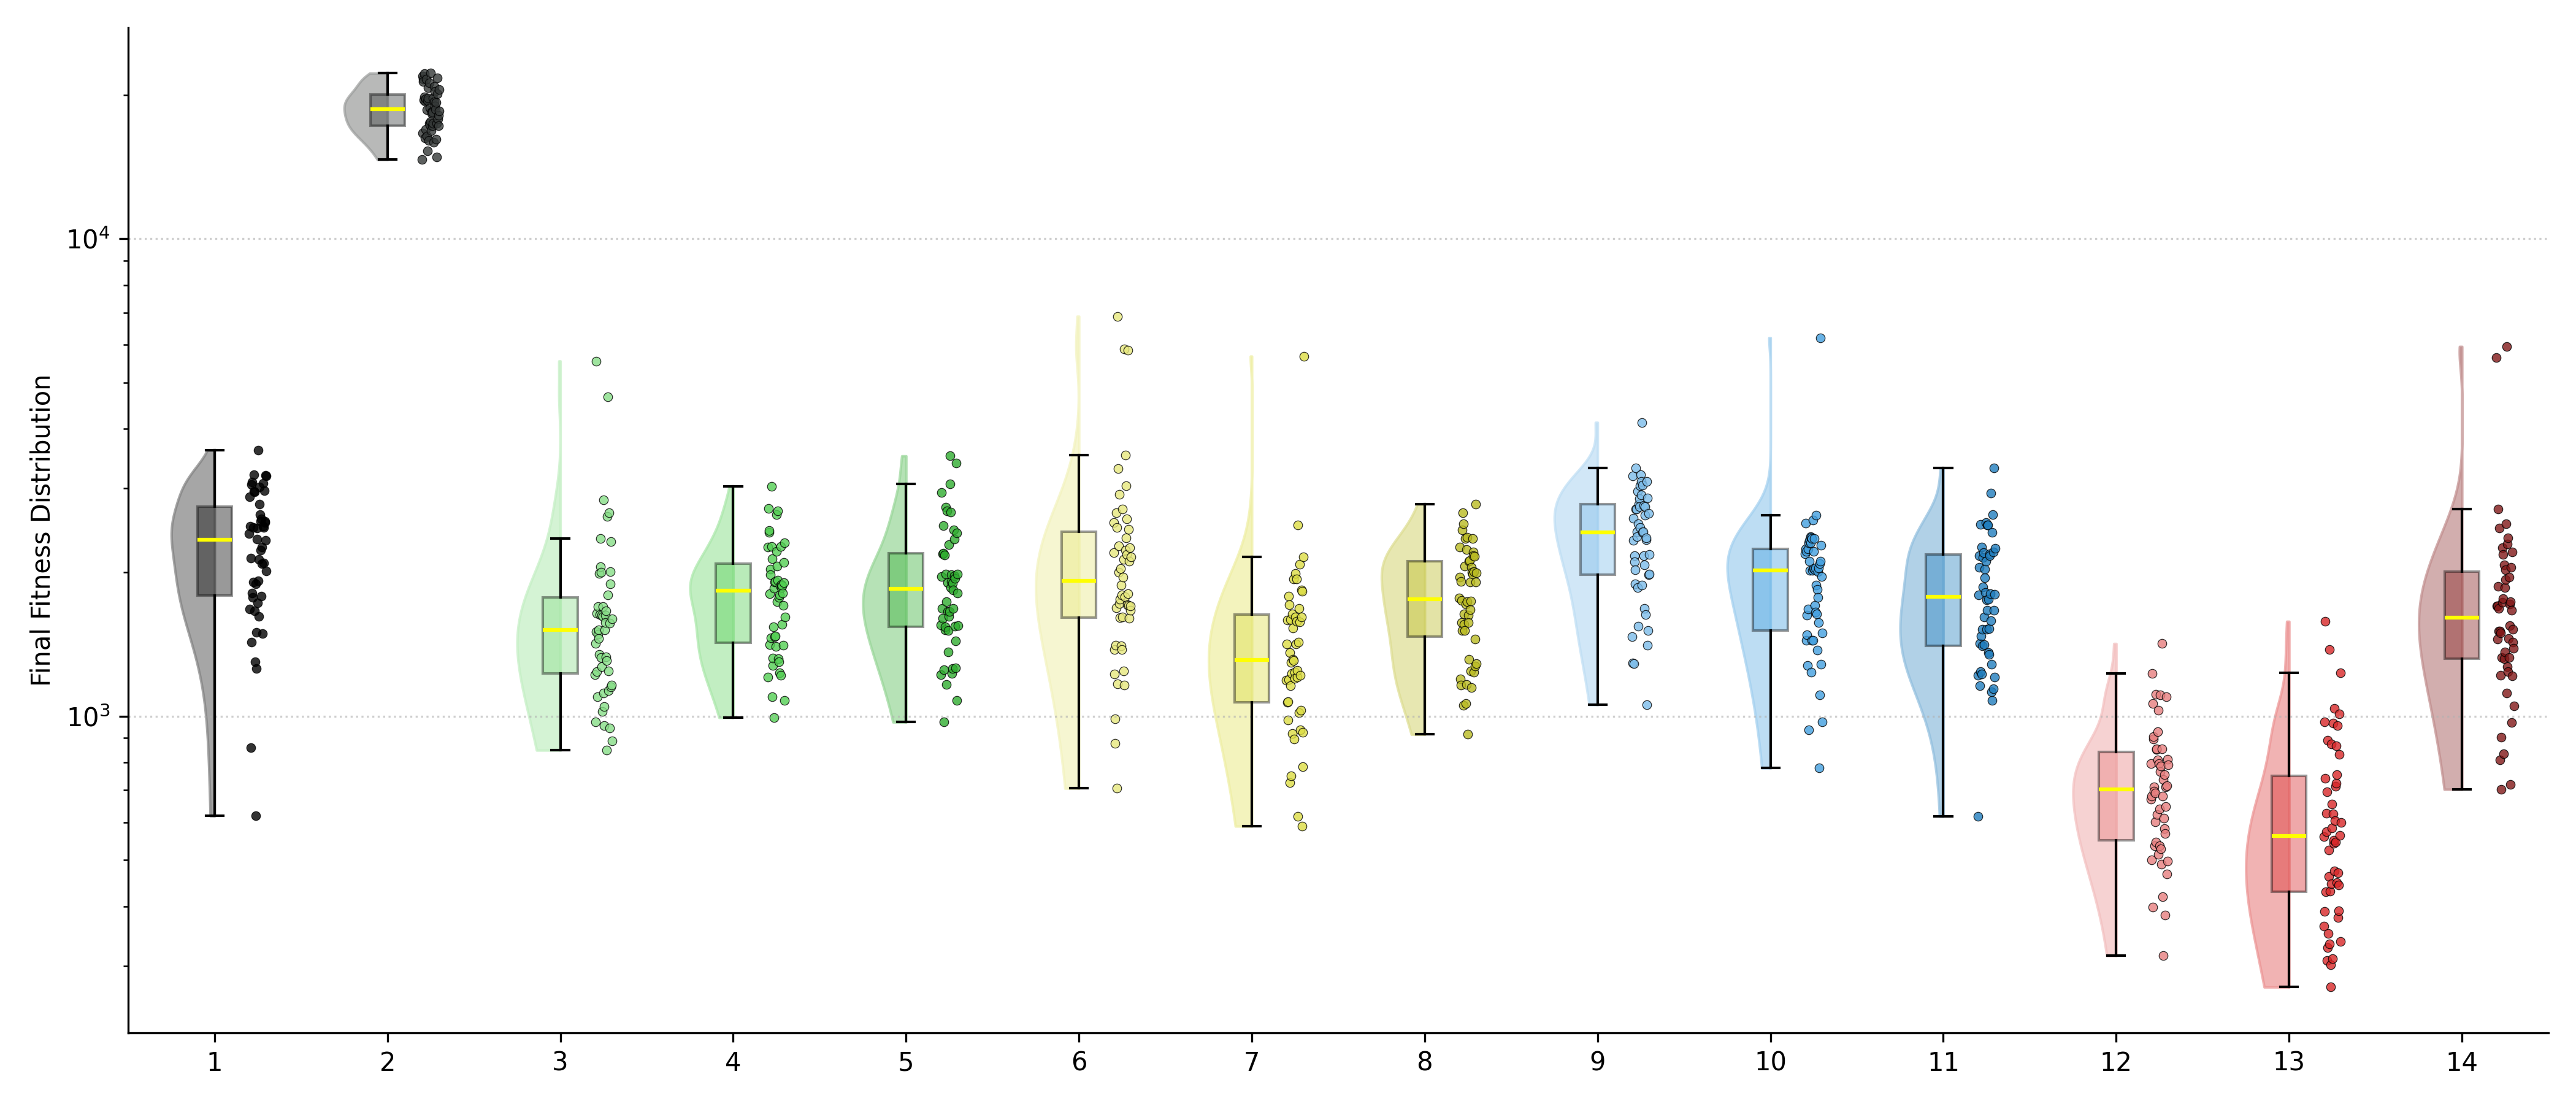
\includegraphics[width=.49\textwidth]{Figures/results/100/Modified_Rosenbrock_No.02___Hollow_Ground_Bent_Knife_Edge_all_dim100_raincloud_vertical.png}
    \caption{Modified Rosenbrock N.2 (log)}
\end{subfigure}

\begin{subfigure}{1\textwidth}
    \centering
    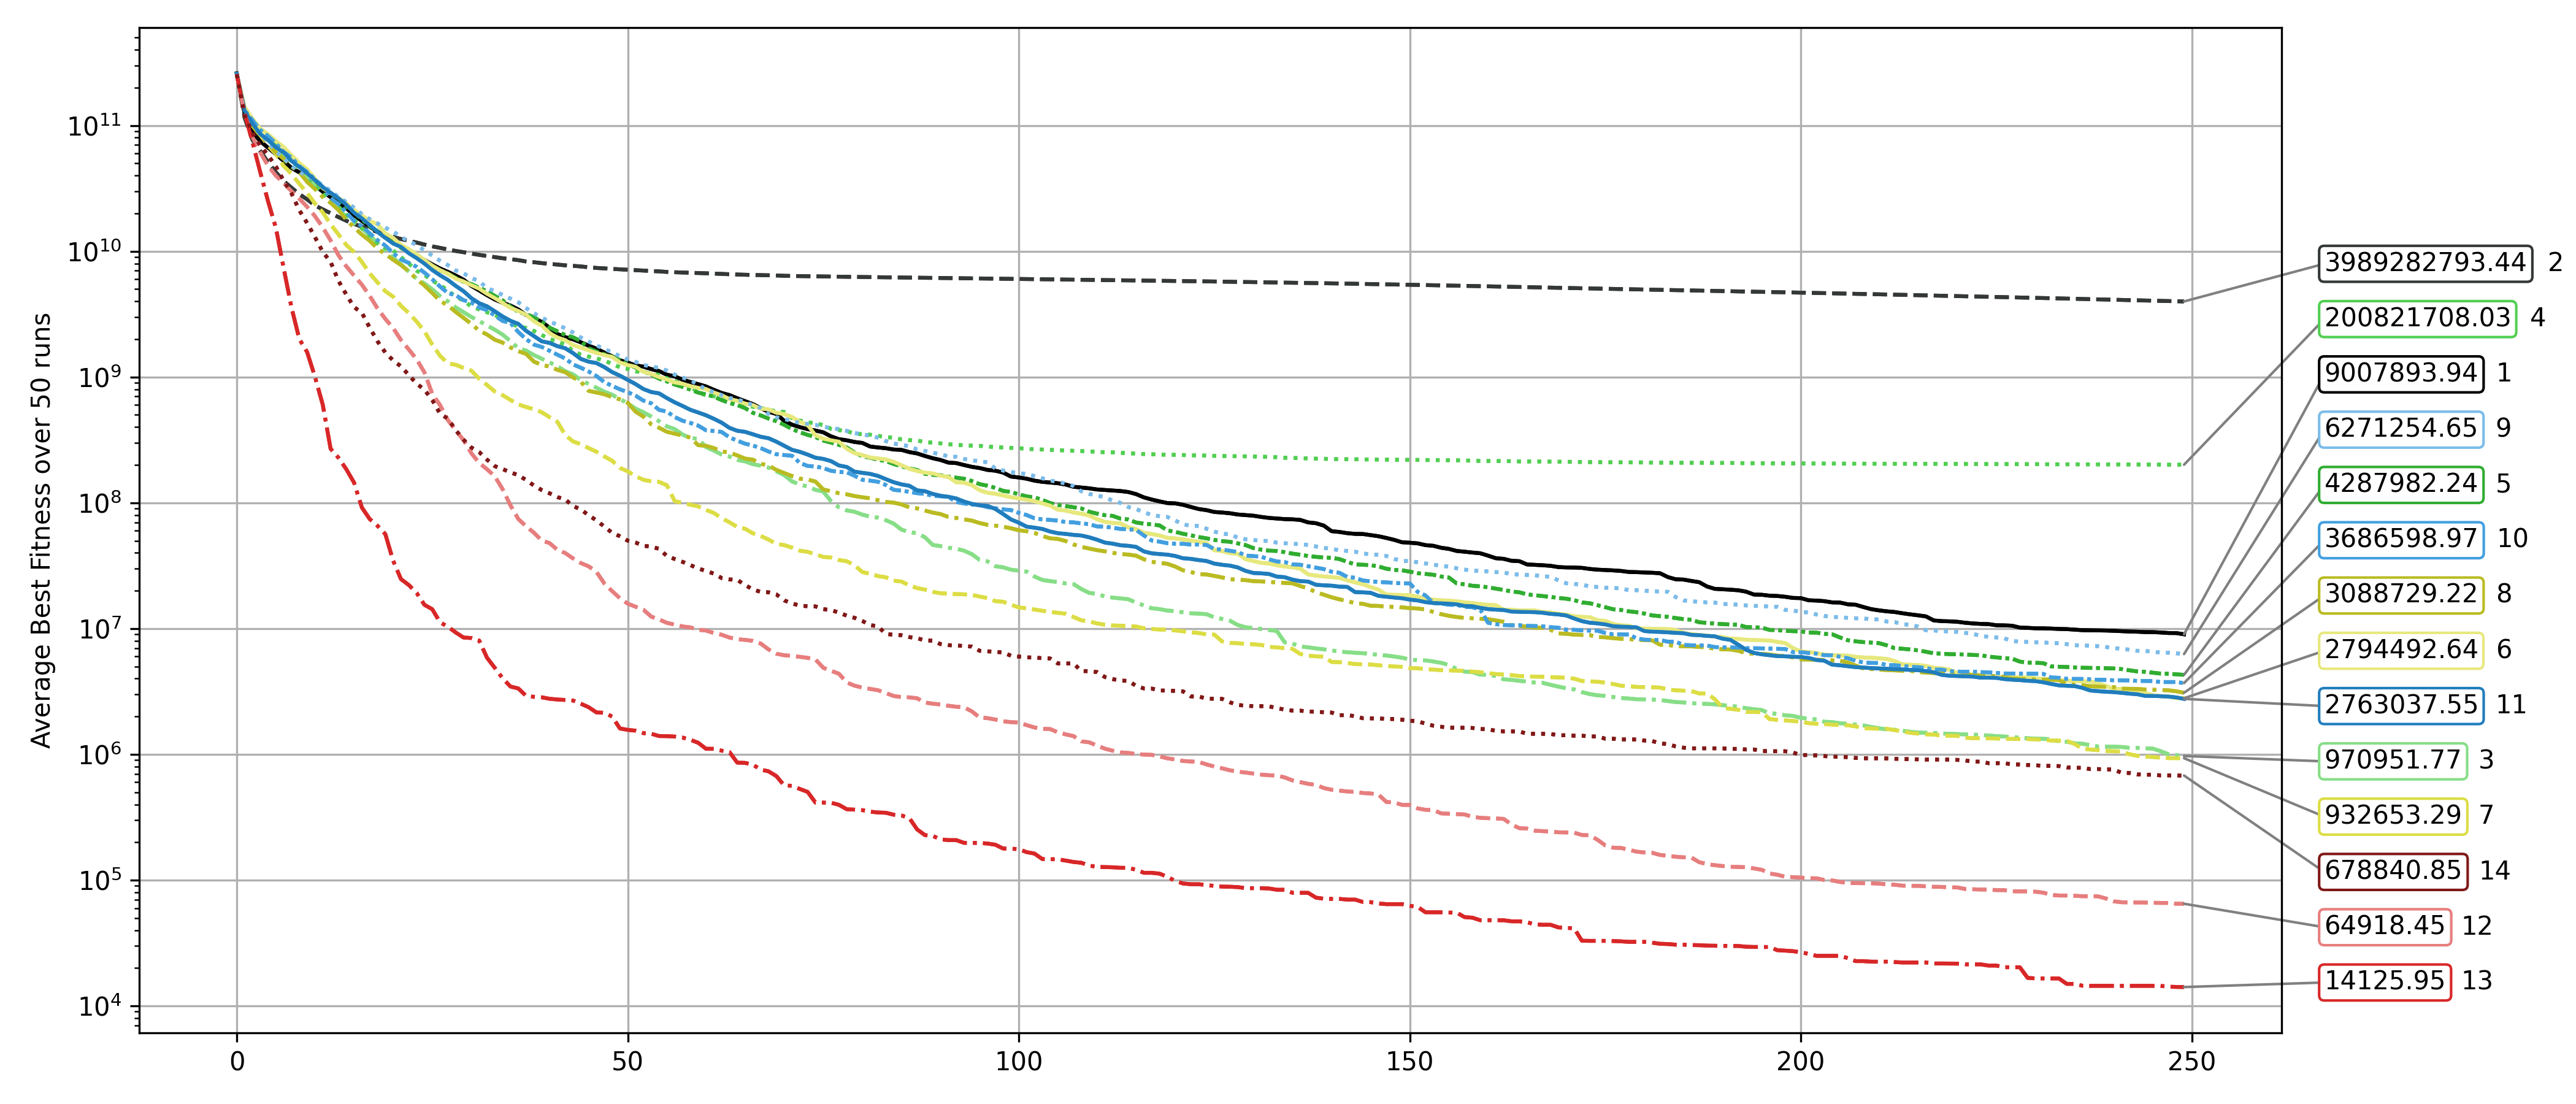
\includegraphics[width=.49\textwidth]{Figures/results/100/Rotated_Bent_Cigar_All_selected_algorithms_dim100_annot_legend.png}
    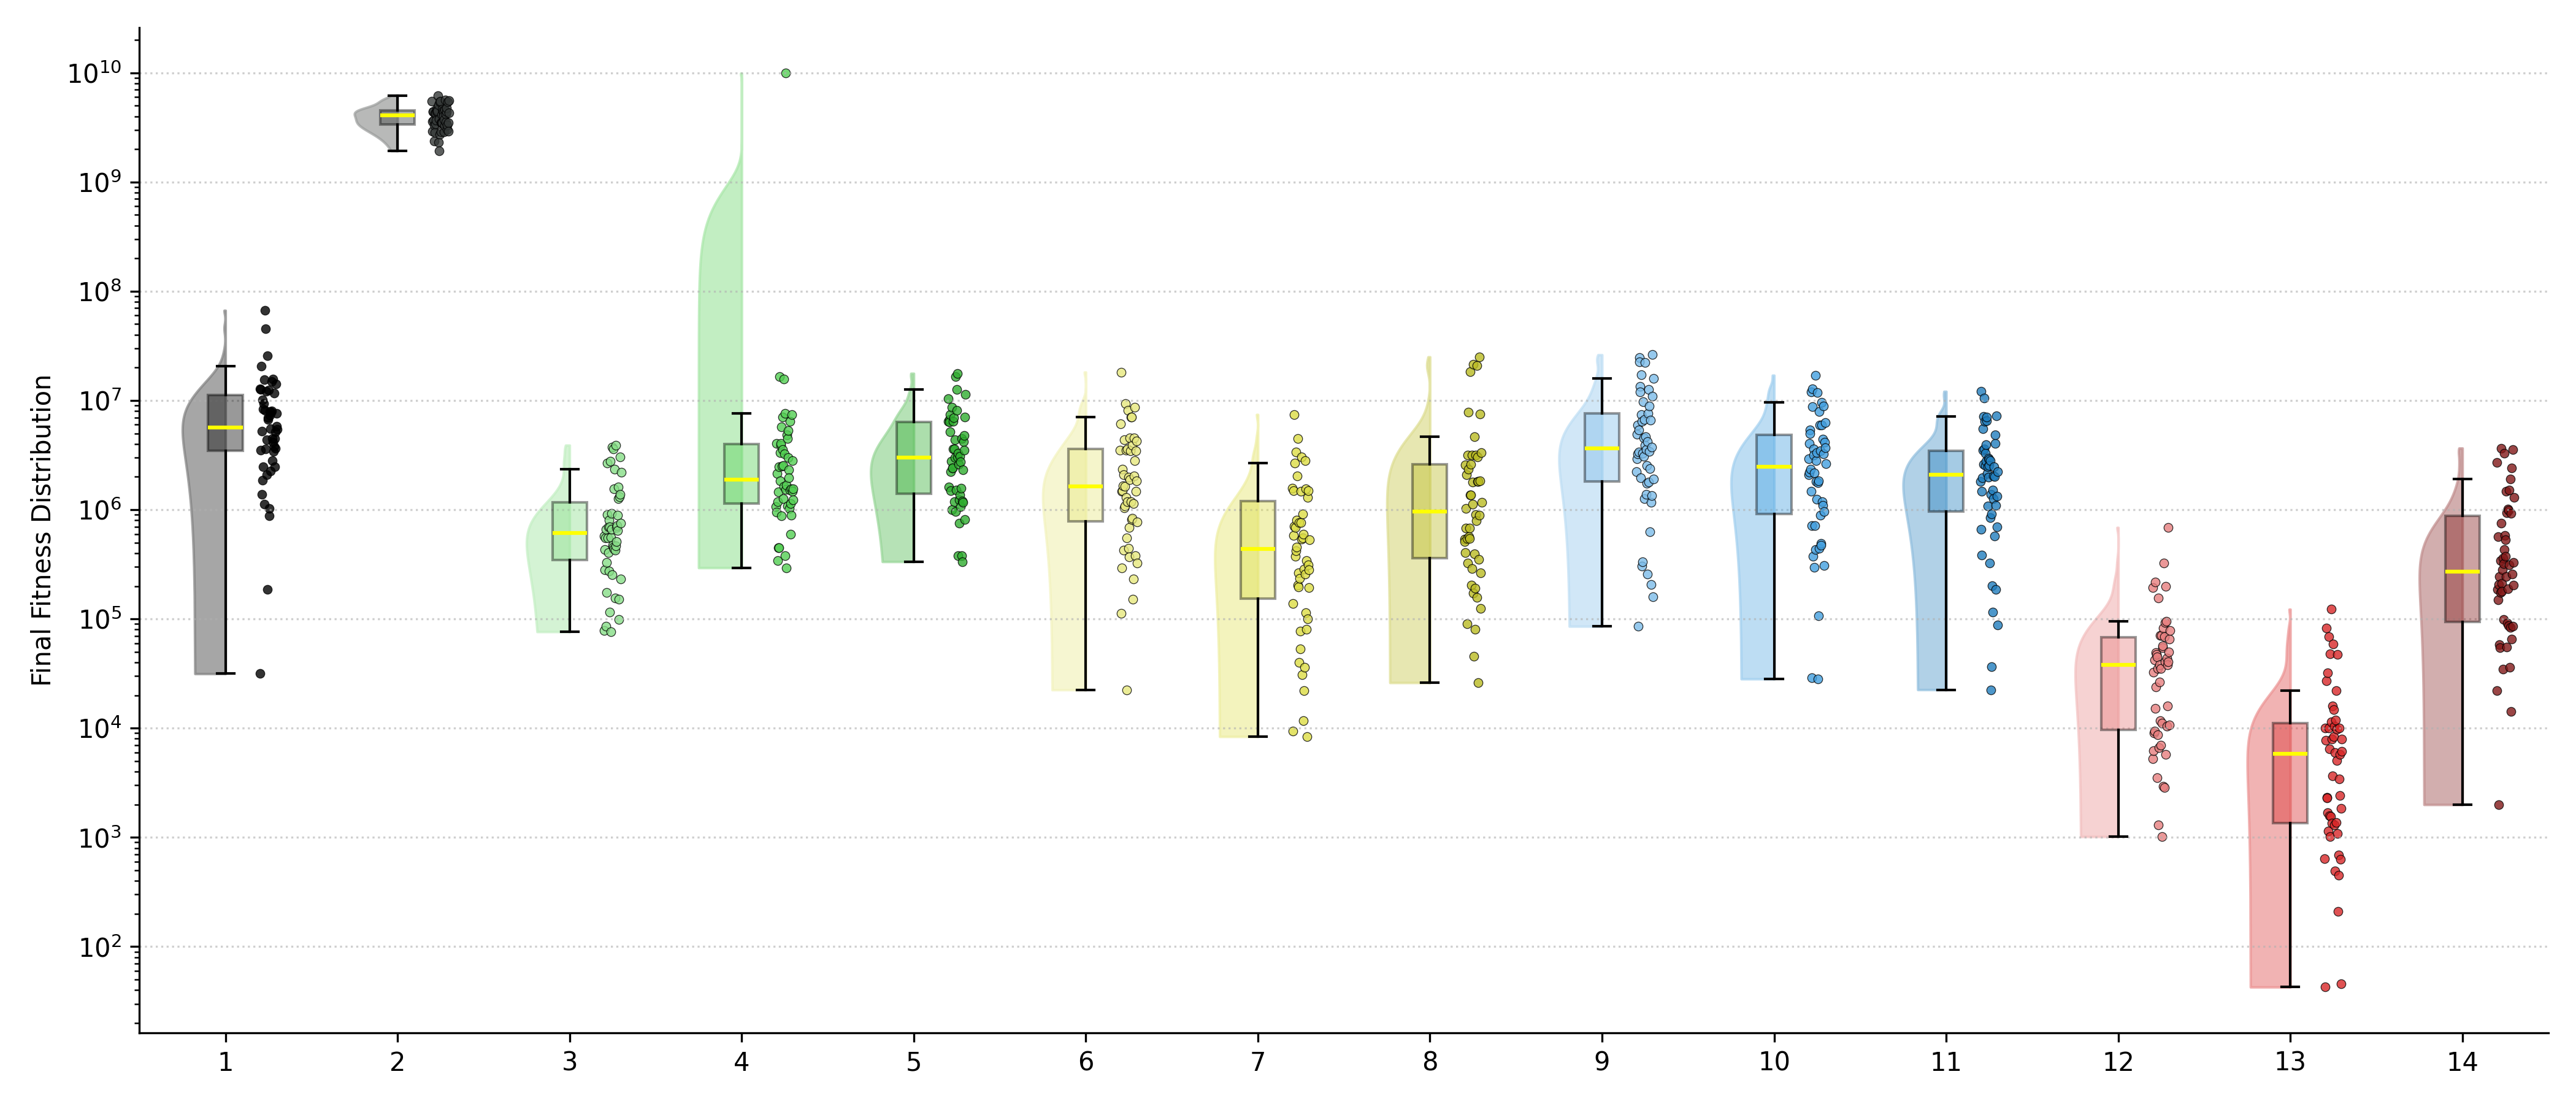
\includegraphics[width=.49\textwidth]{Figures/results/100/Rotated_Bent_Cigar_all_dim100_raincloud_vertical.png}
    \caption{Rotated Bent Cigar (log)}
\end{subfigure}

\begin{subfigure}{1\textwidth}
    \centering
    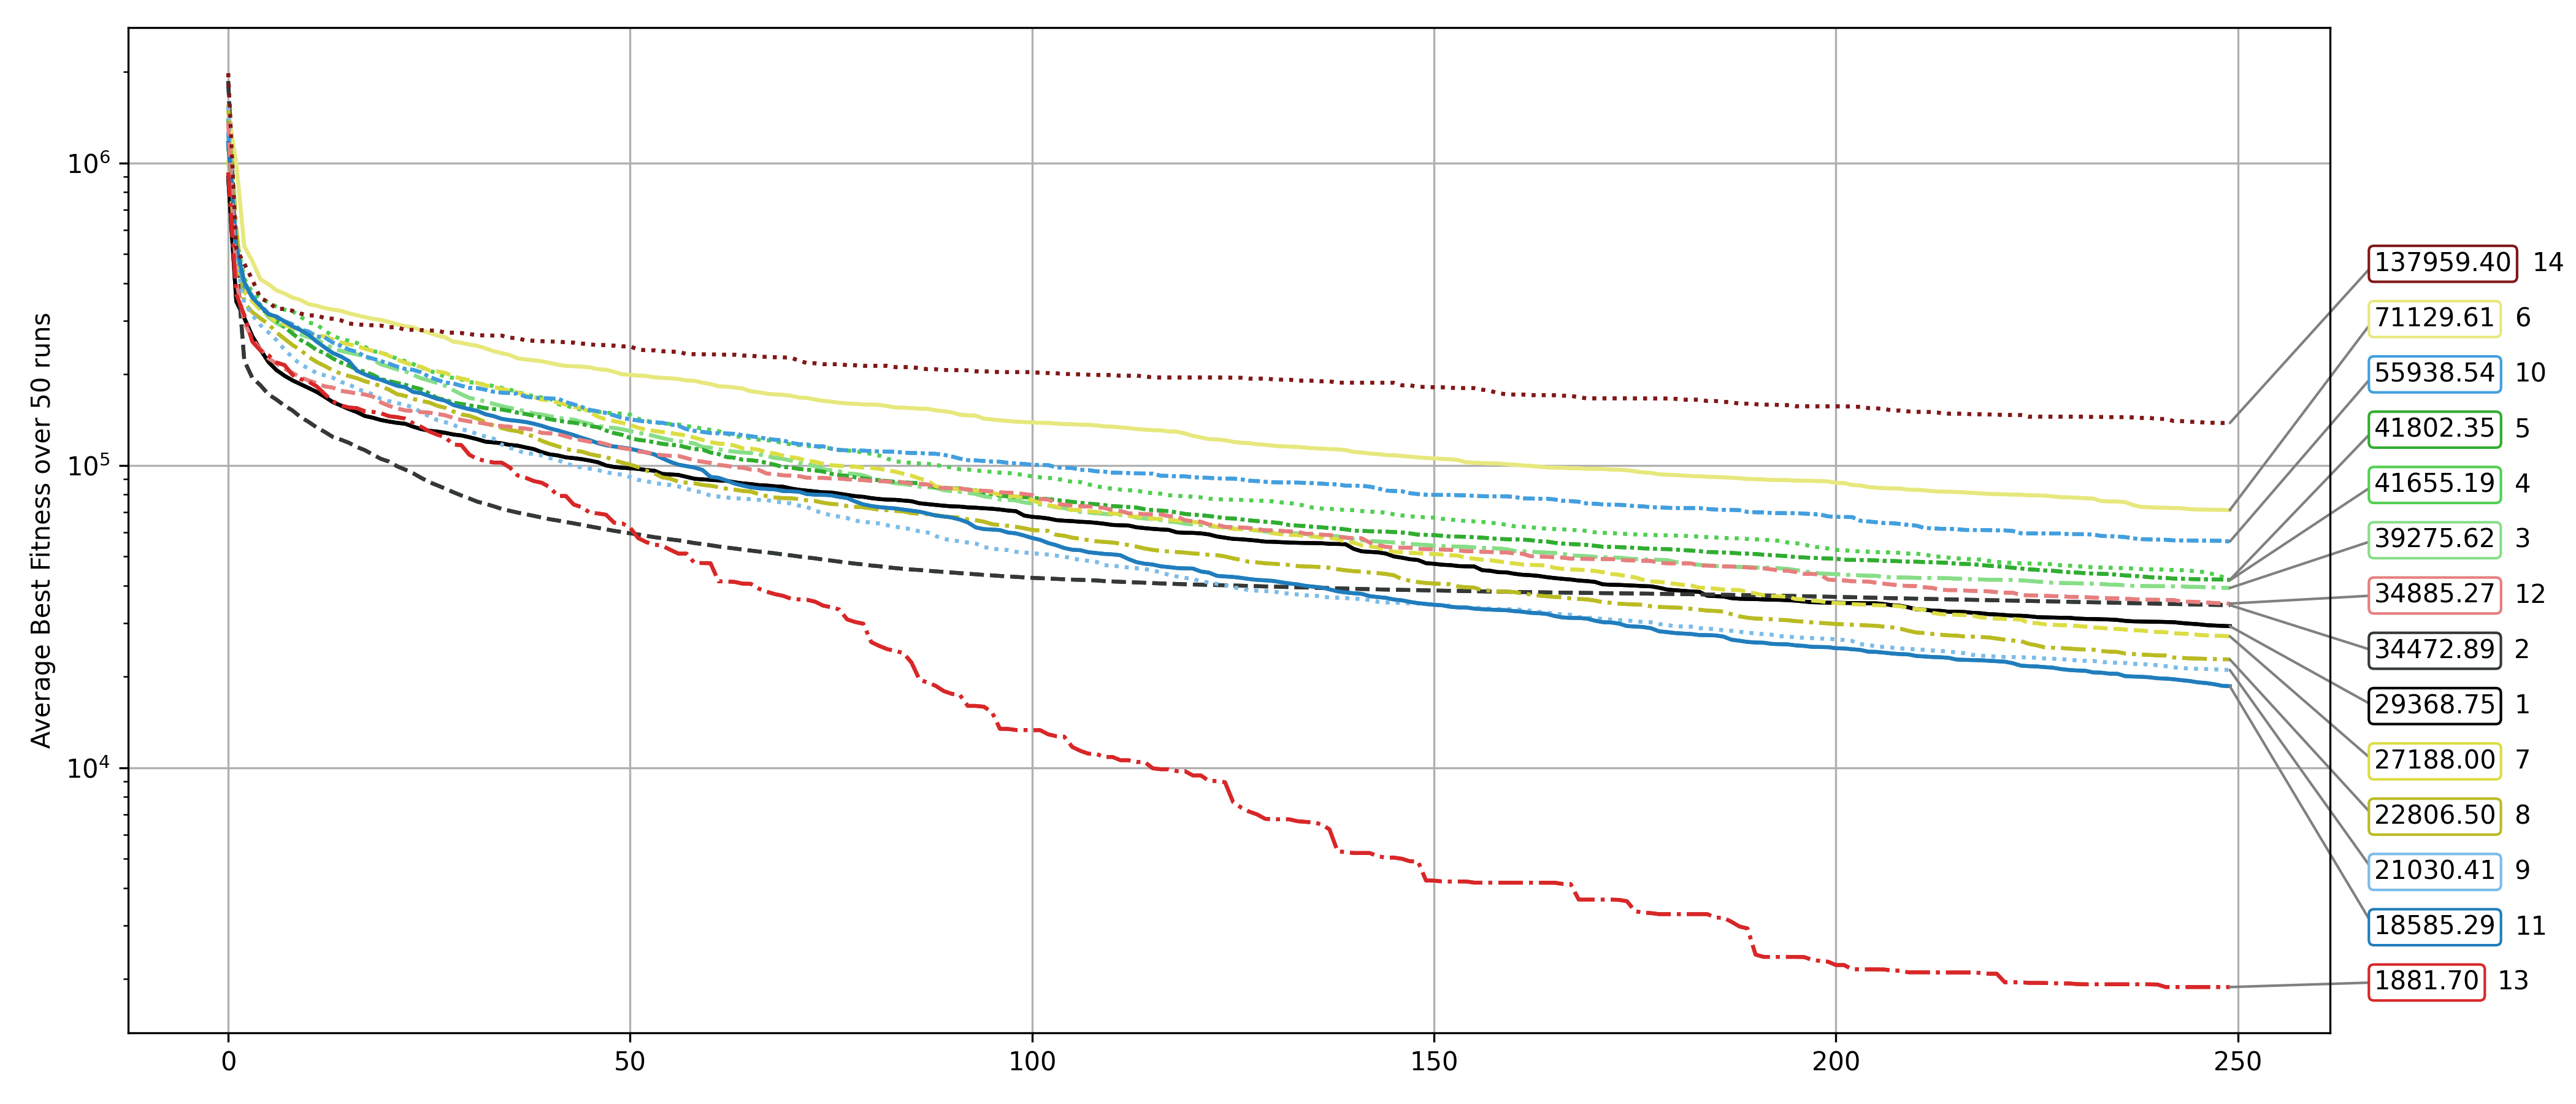
\includegraphics[width=.49\textwidth]{Figures/results/100/Rotated_Discus_All_selected_algorithms_dim100_annot_legend.png}
    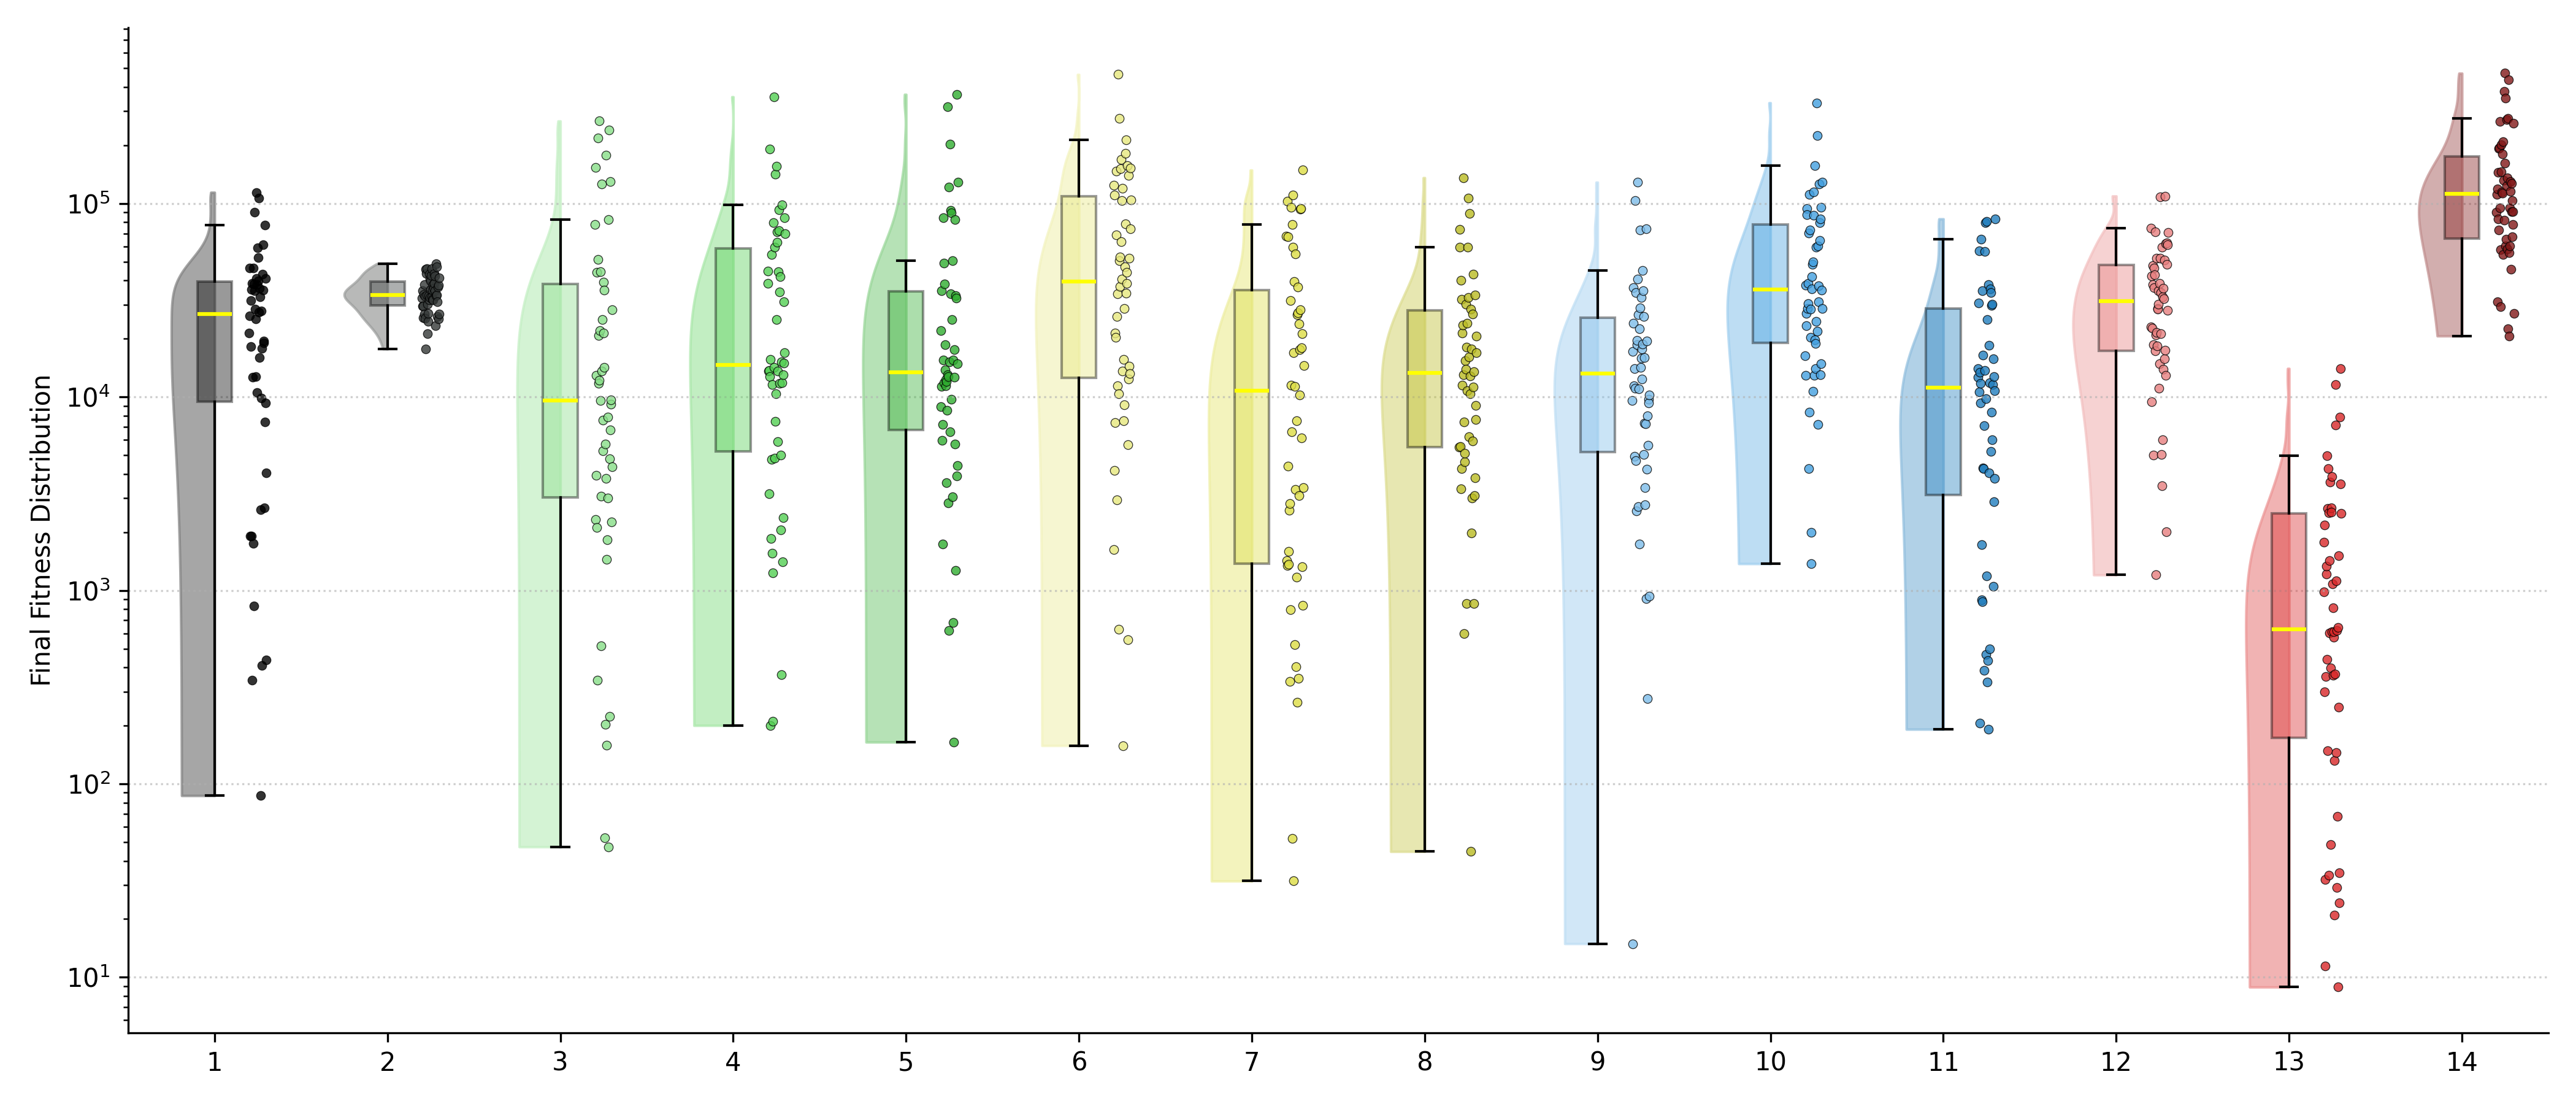
\includegraphics[width=.49\textwidth]{Figures/results/100/Rotated_Discus_all_dim100_raincloud_vertical.png}
    \caption{Rotated Discus (log)}
\end{subfigure}

\begin{subfigure}{1\textwidth}
    \centering
    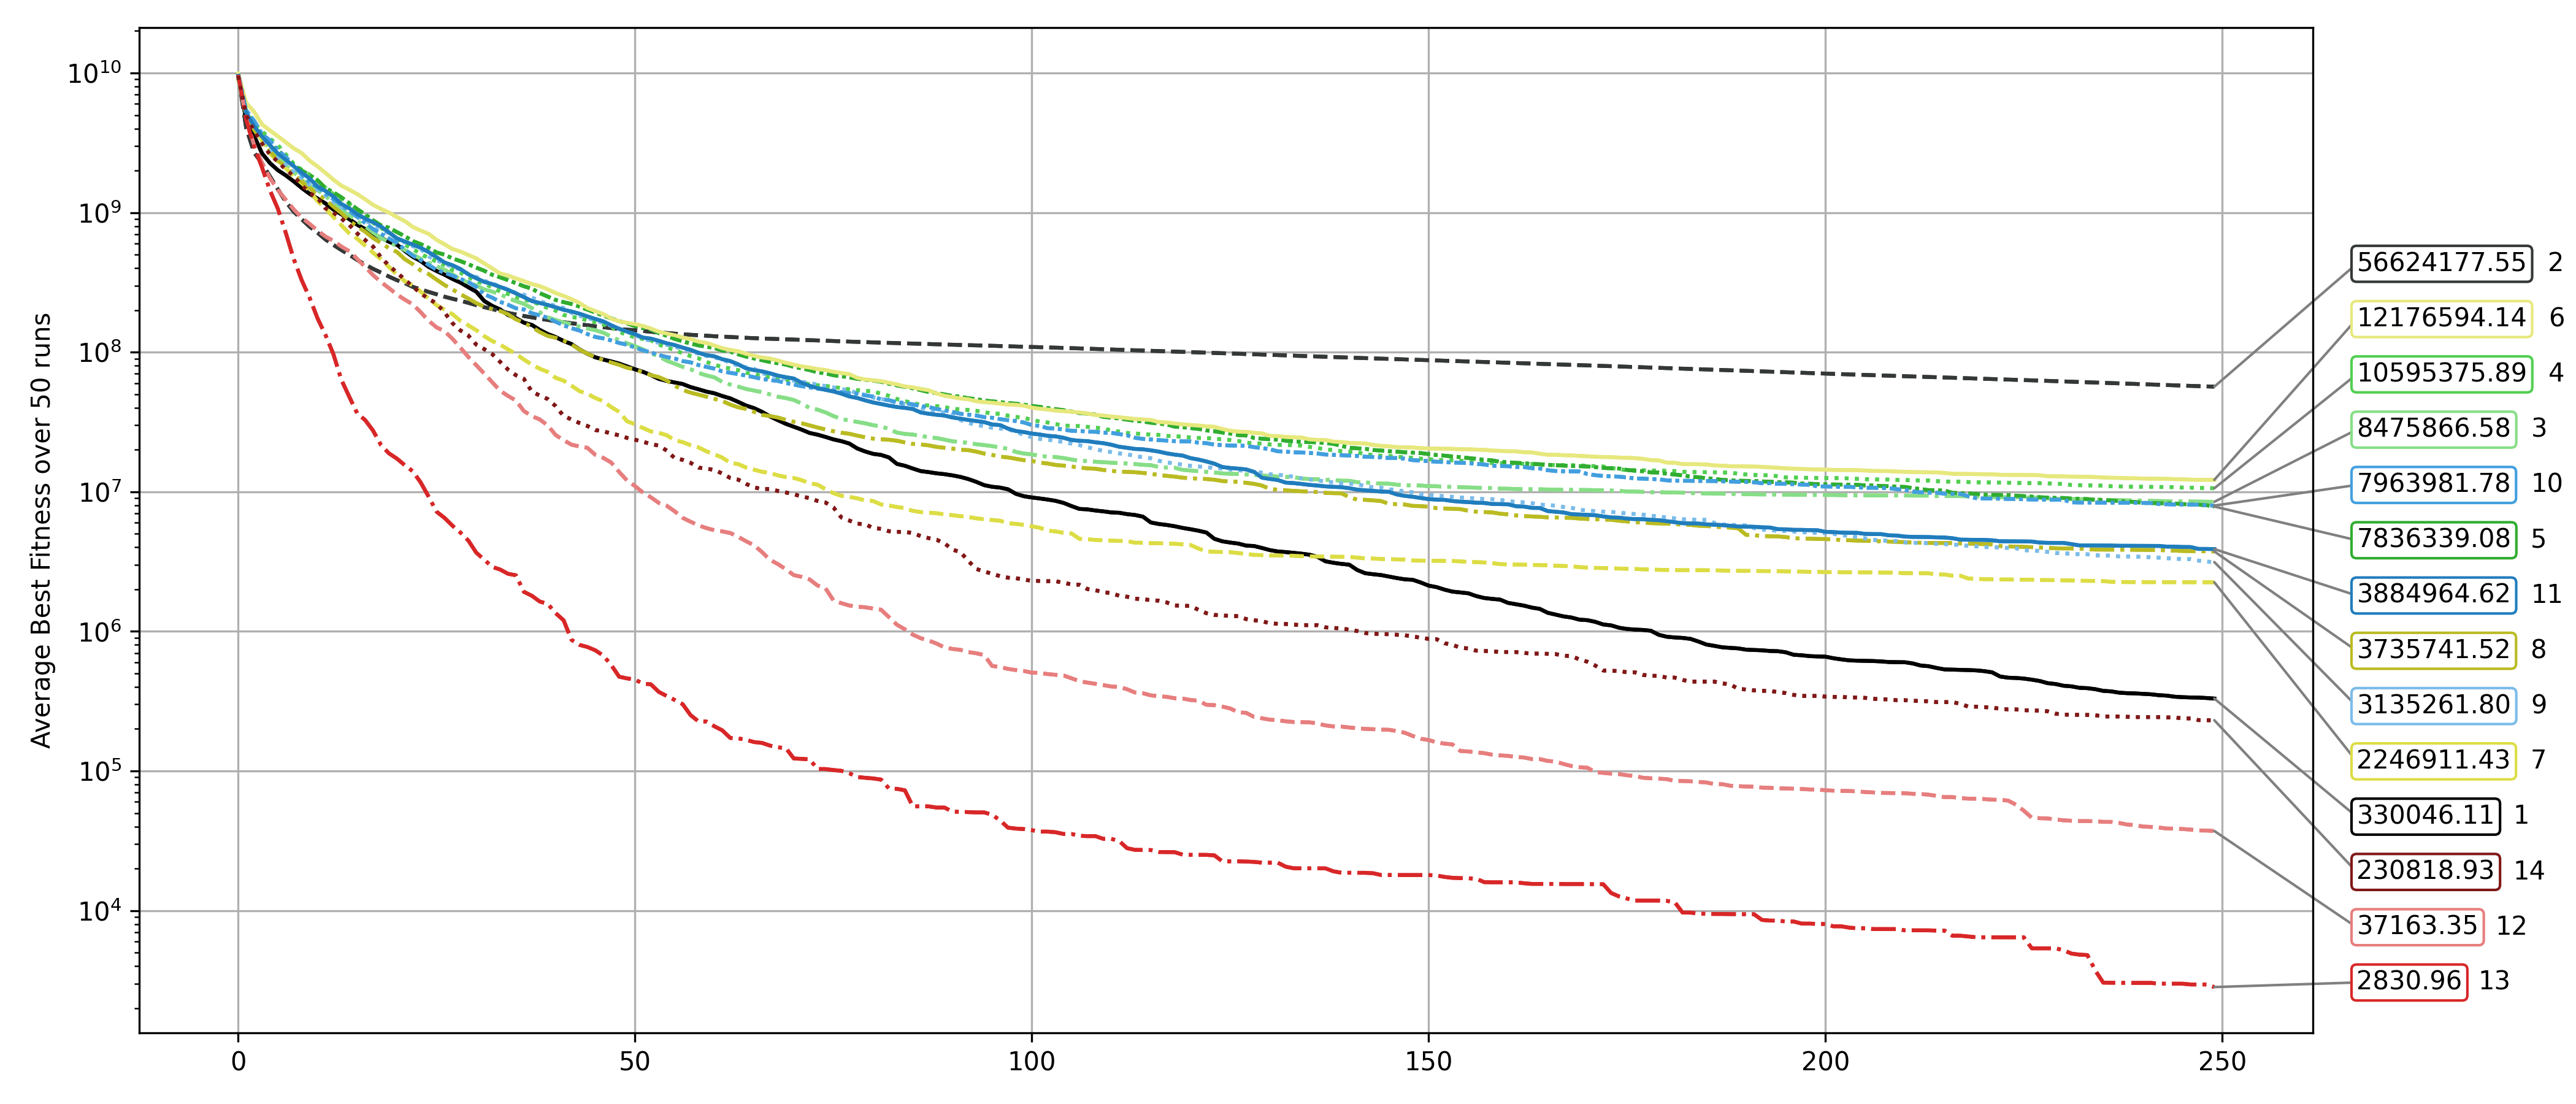
\includegraphics[width=.49\textwidth]{Figures/results/100/Rotated_High_Conditioned_Elliptic_All_selected_algorithms_dim100_annot_legend.png}
    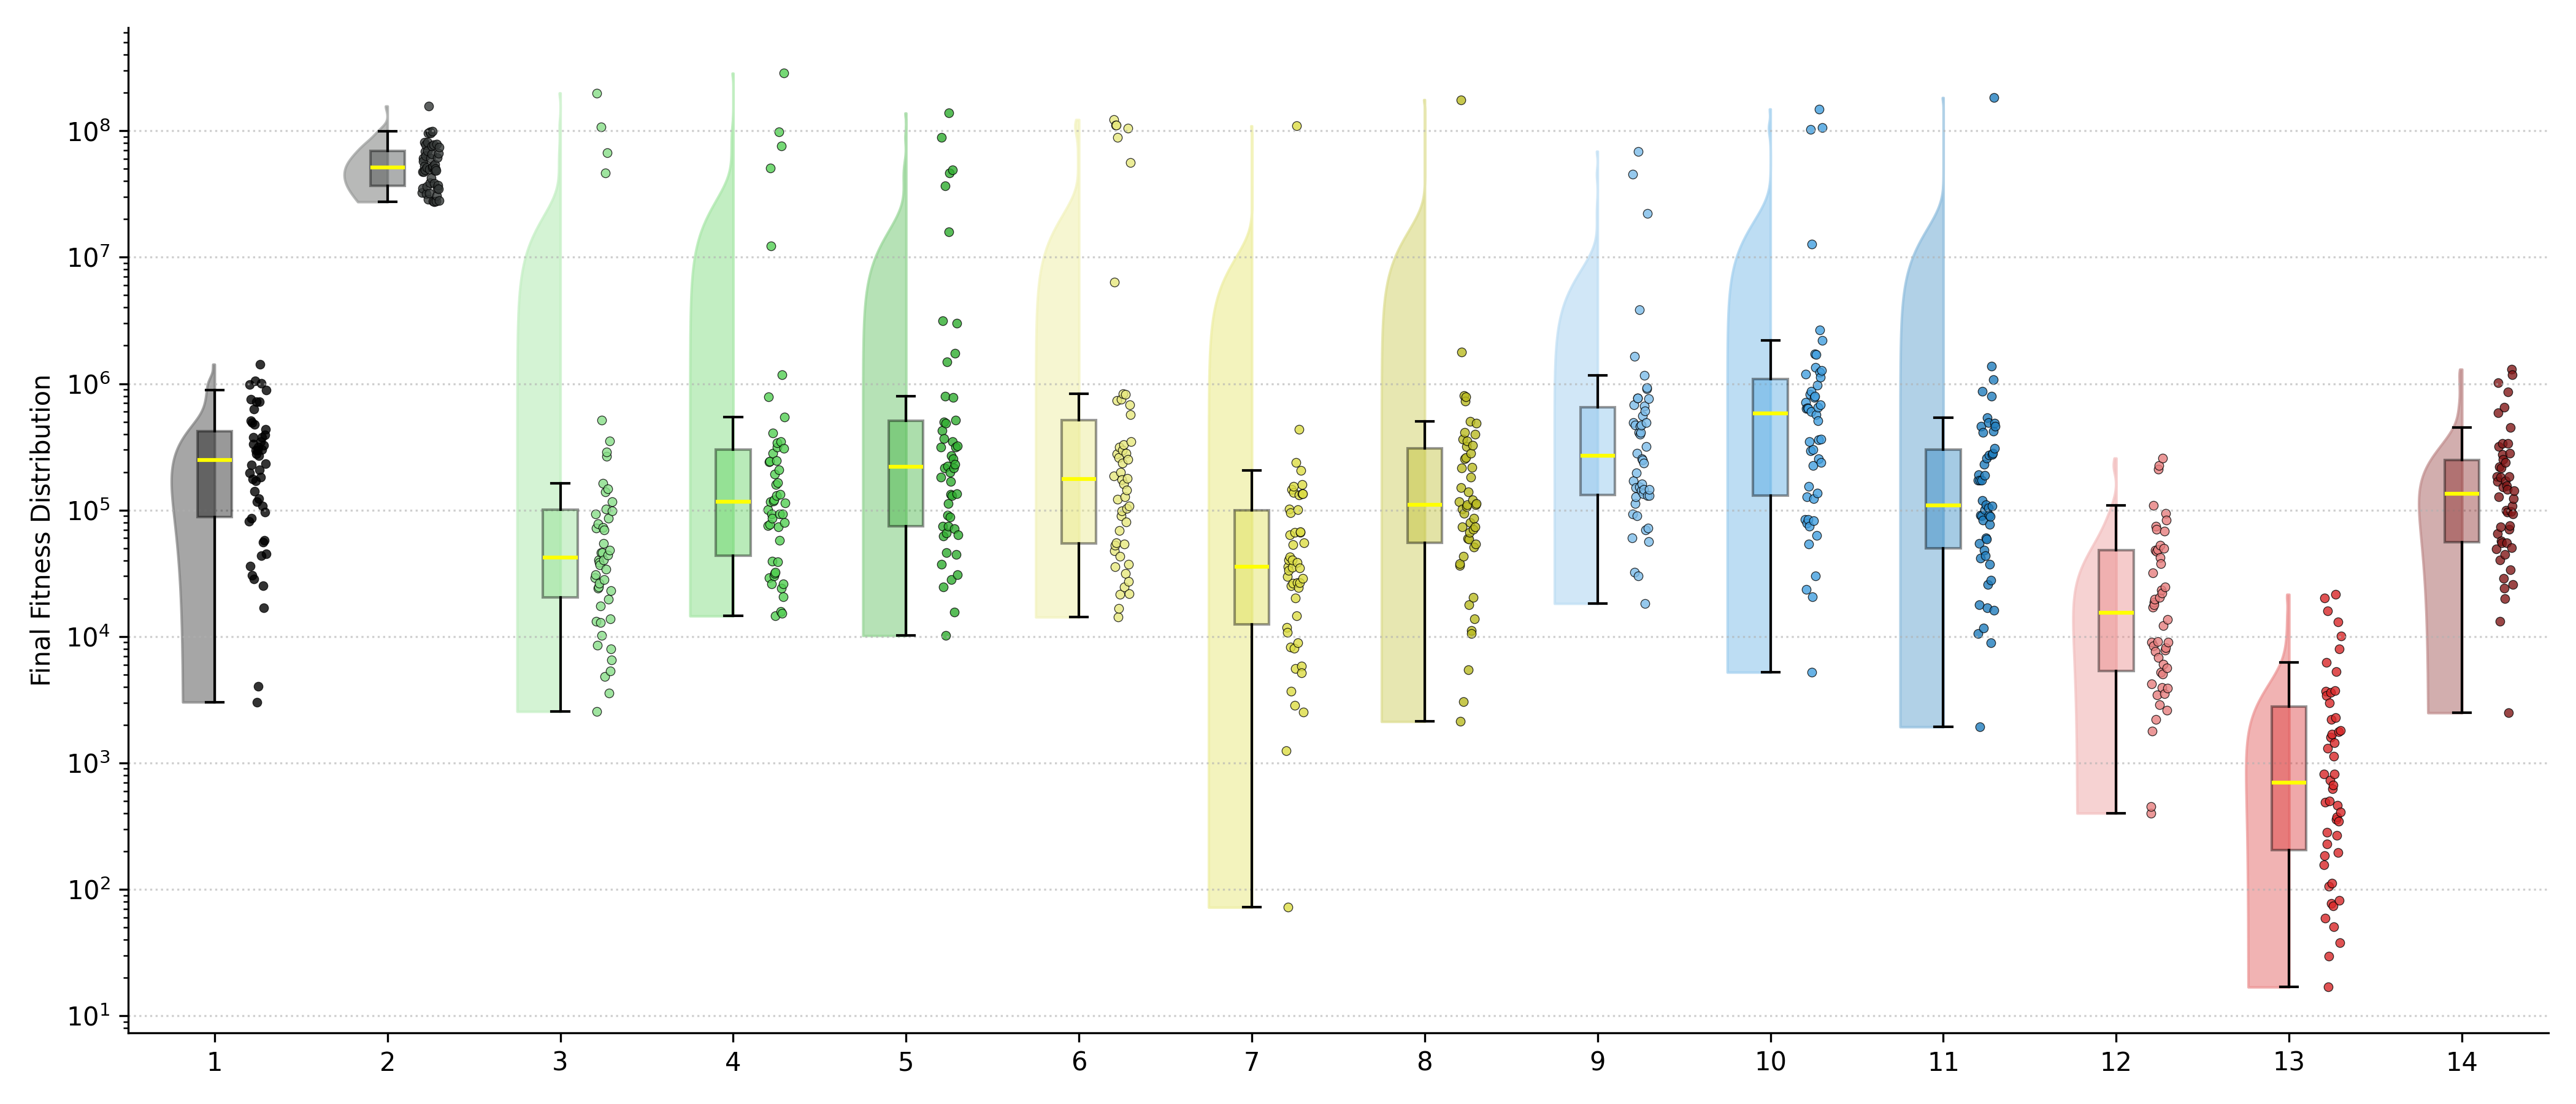
\includegraphics[width=.49\textwidth]{Figures/results/100/Rotated_High_Conditioned_Elliptic_all_dim100_raincloud_vertical.png}
    \caption{Rotated High Conditioned Elliptic (log)}
\end{subfigure}

\begin{subfigure}{1\textwidth}
    \centering
    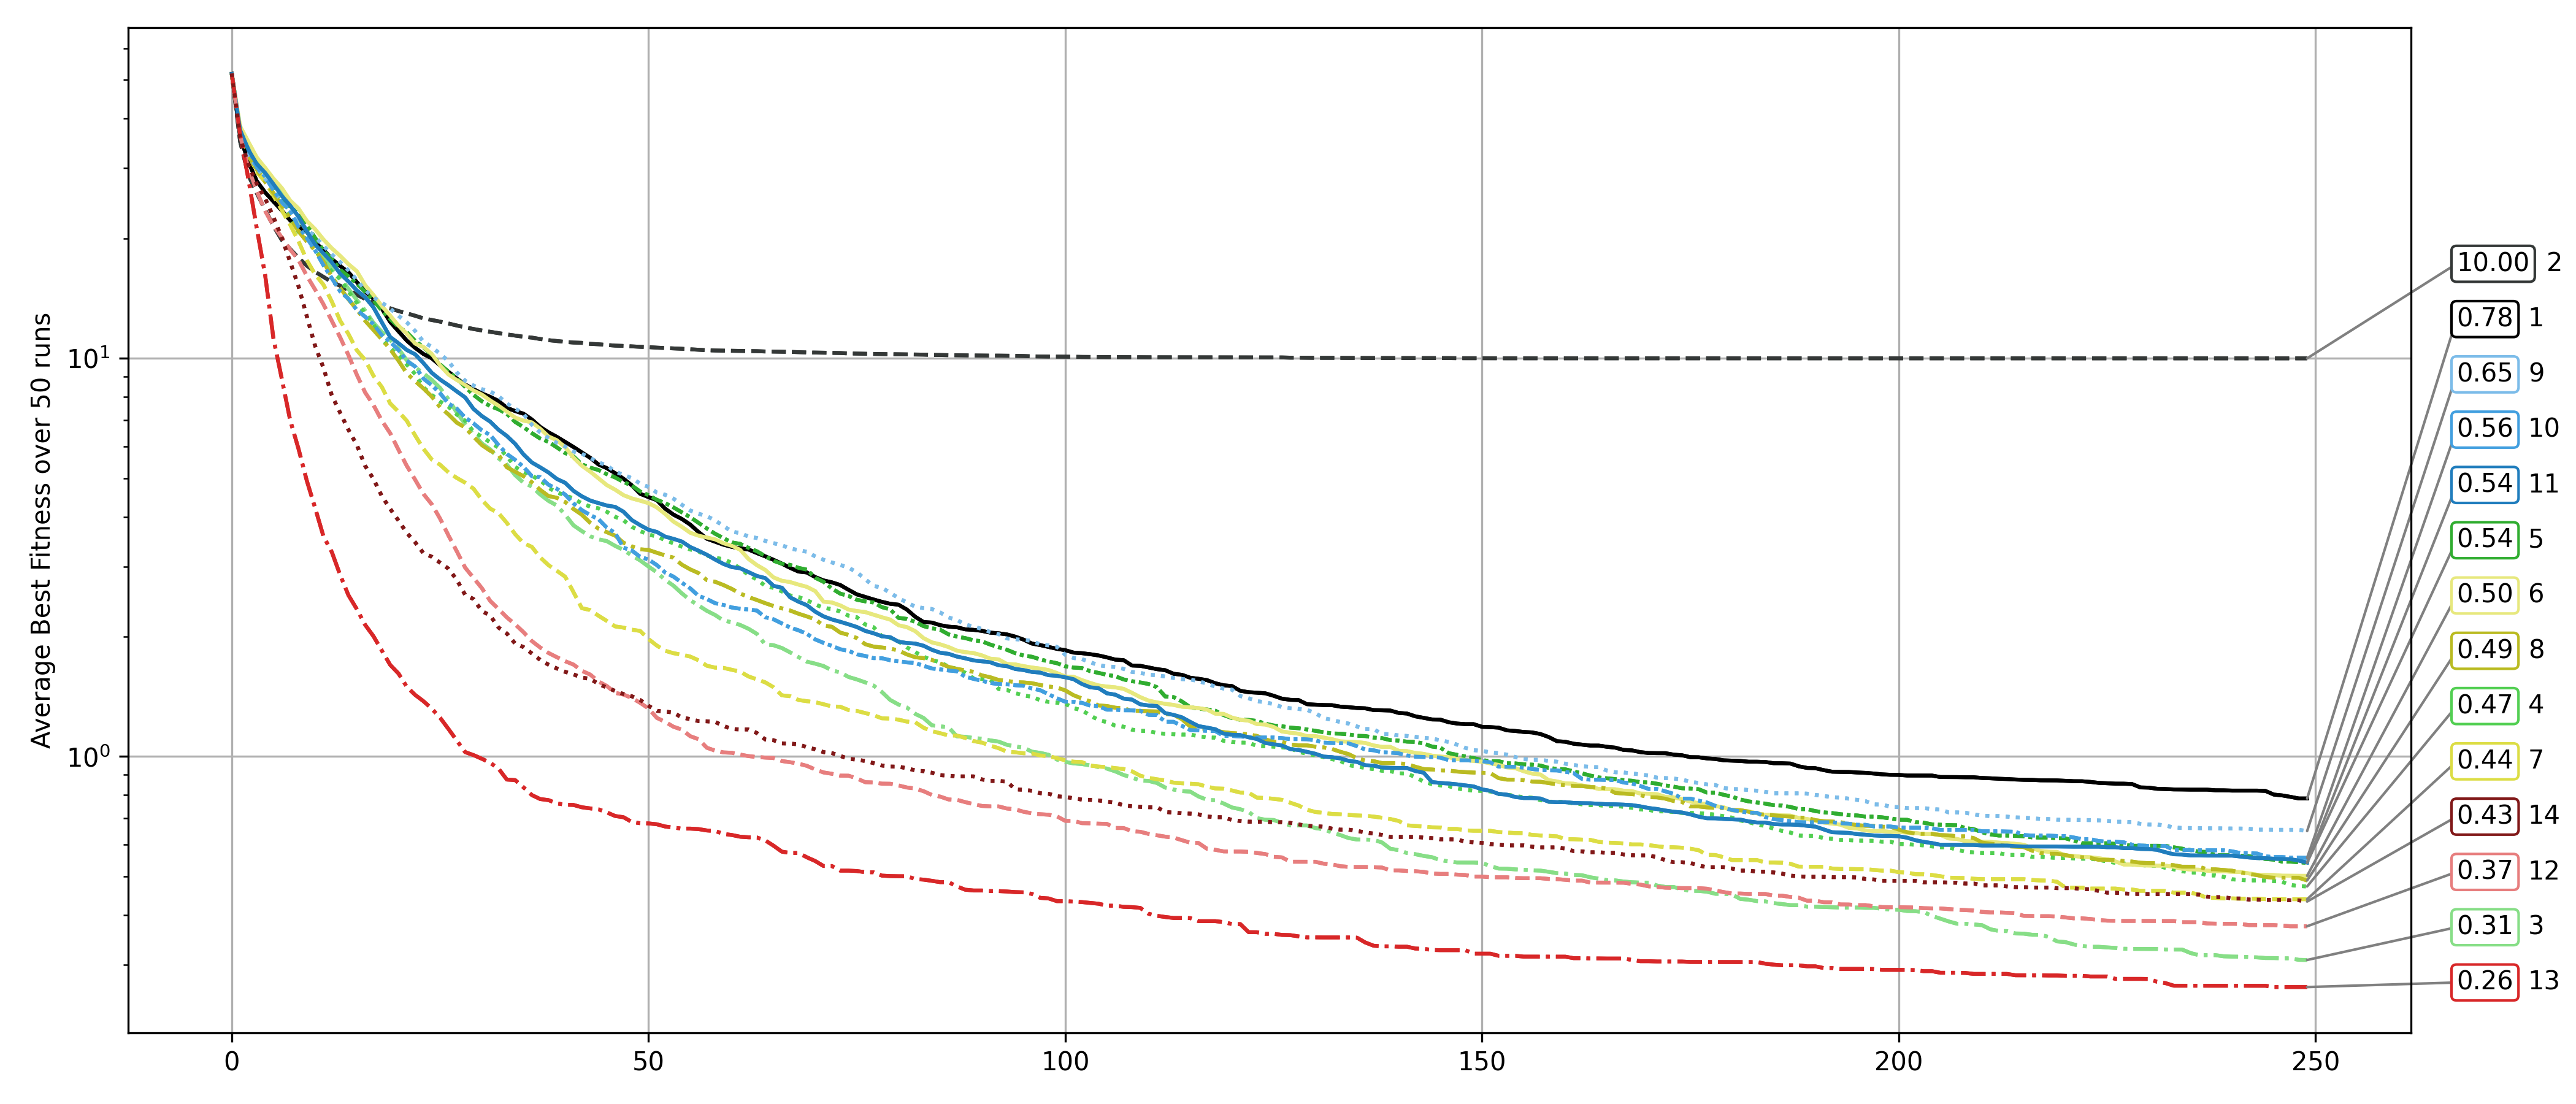
\includegraphics[width=.49\textwidth]{Figures/results/100/Salomon_All_selected_algorithms_dim100_annot_legend.png}
    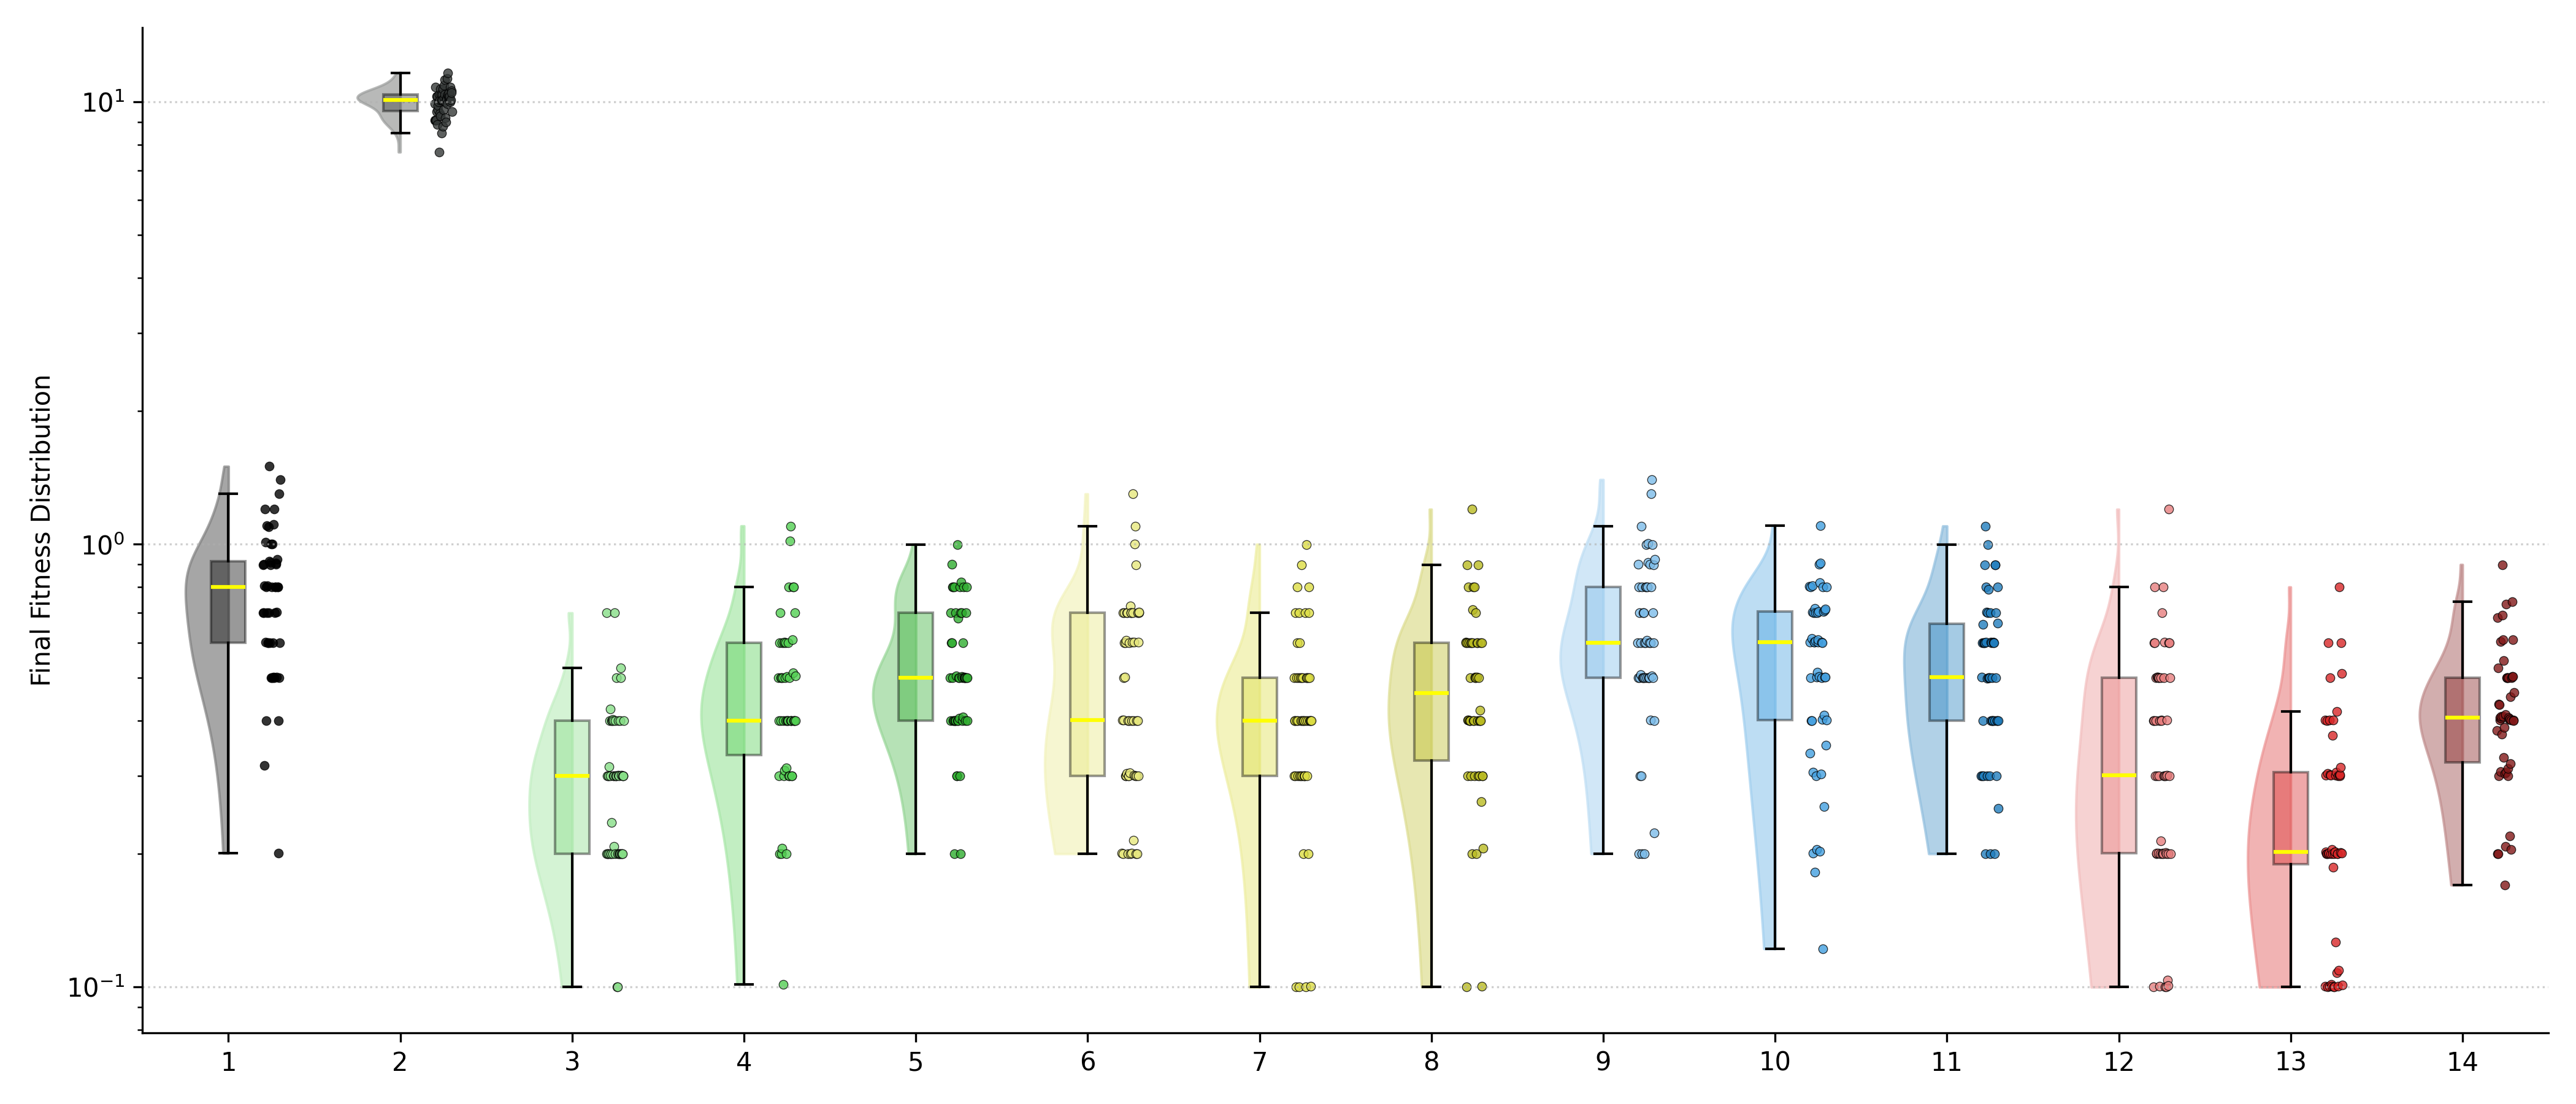
\includegraphics[width=.49\textwidth]{Figures/results/100/Salomon_all_dim100_raincloud_vertical.png}
    \caption{Salomon (log)}
\end{subfigure}

    \captionsetup{list=no}
\caption[Convergence curves and final fitness distribution raincloud plots for 100-dimensional problems]{Convergence curves (left) and final fitness distribution raincloud plots (right) for each tested benchmark problem in the 100-dimensional setting. Algorithms are numbered, line-styled, ordered, and color-coded consistently according to the legend in Figure~\ref{fig:plot_encoding}. Problems plotted on a logarithmic scale are indicated with ``(log)'' following the problem name.}
\end{figure}


%%%%%%%%%


\begin{figure}[p]\ContinuedFloat
\renewcommand\thesubfigure{C.\arabic{figure}.\arabic{subfigure}} % Local change starts here

    \centering

\begin{subfigure}{1\textwidth}
    \centering
    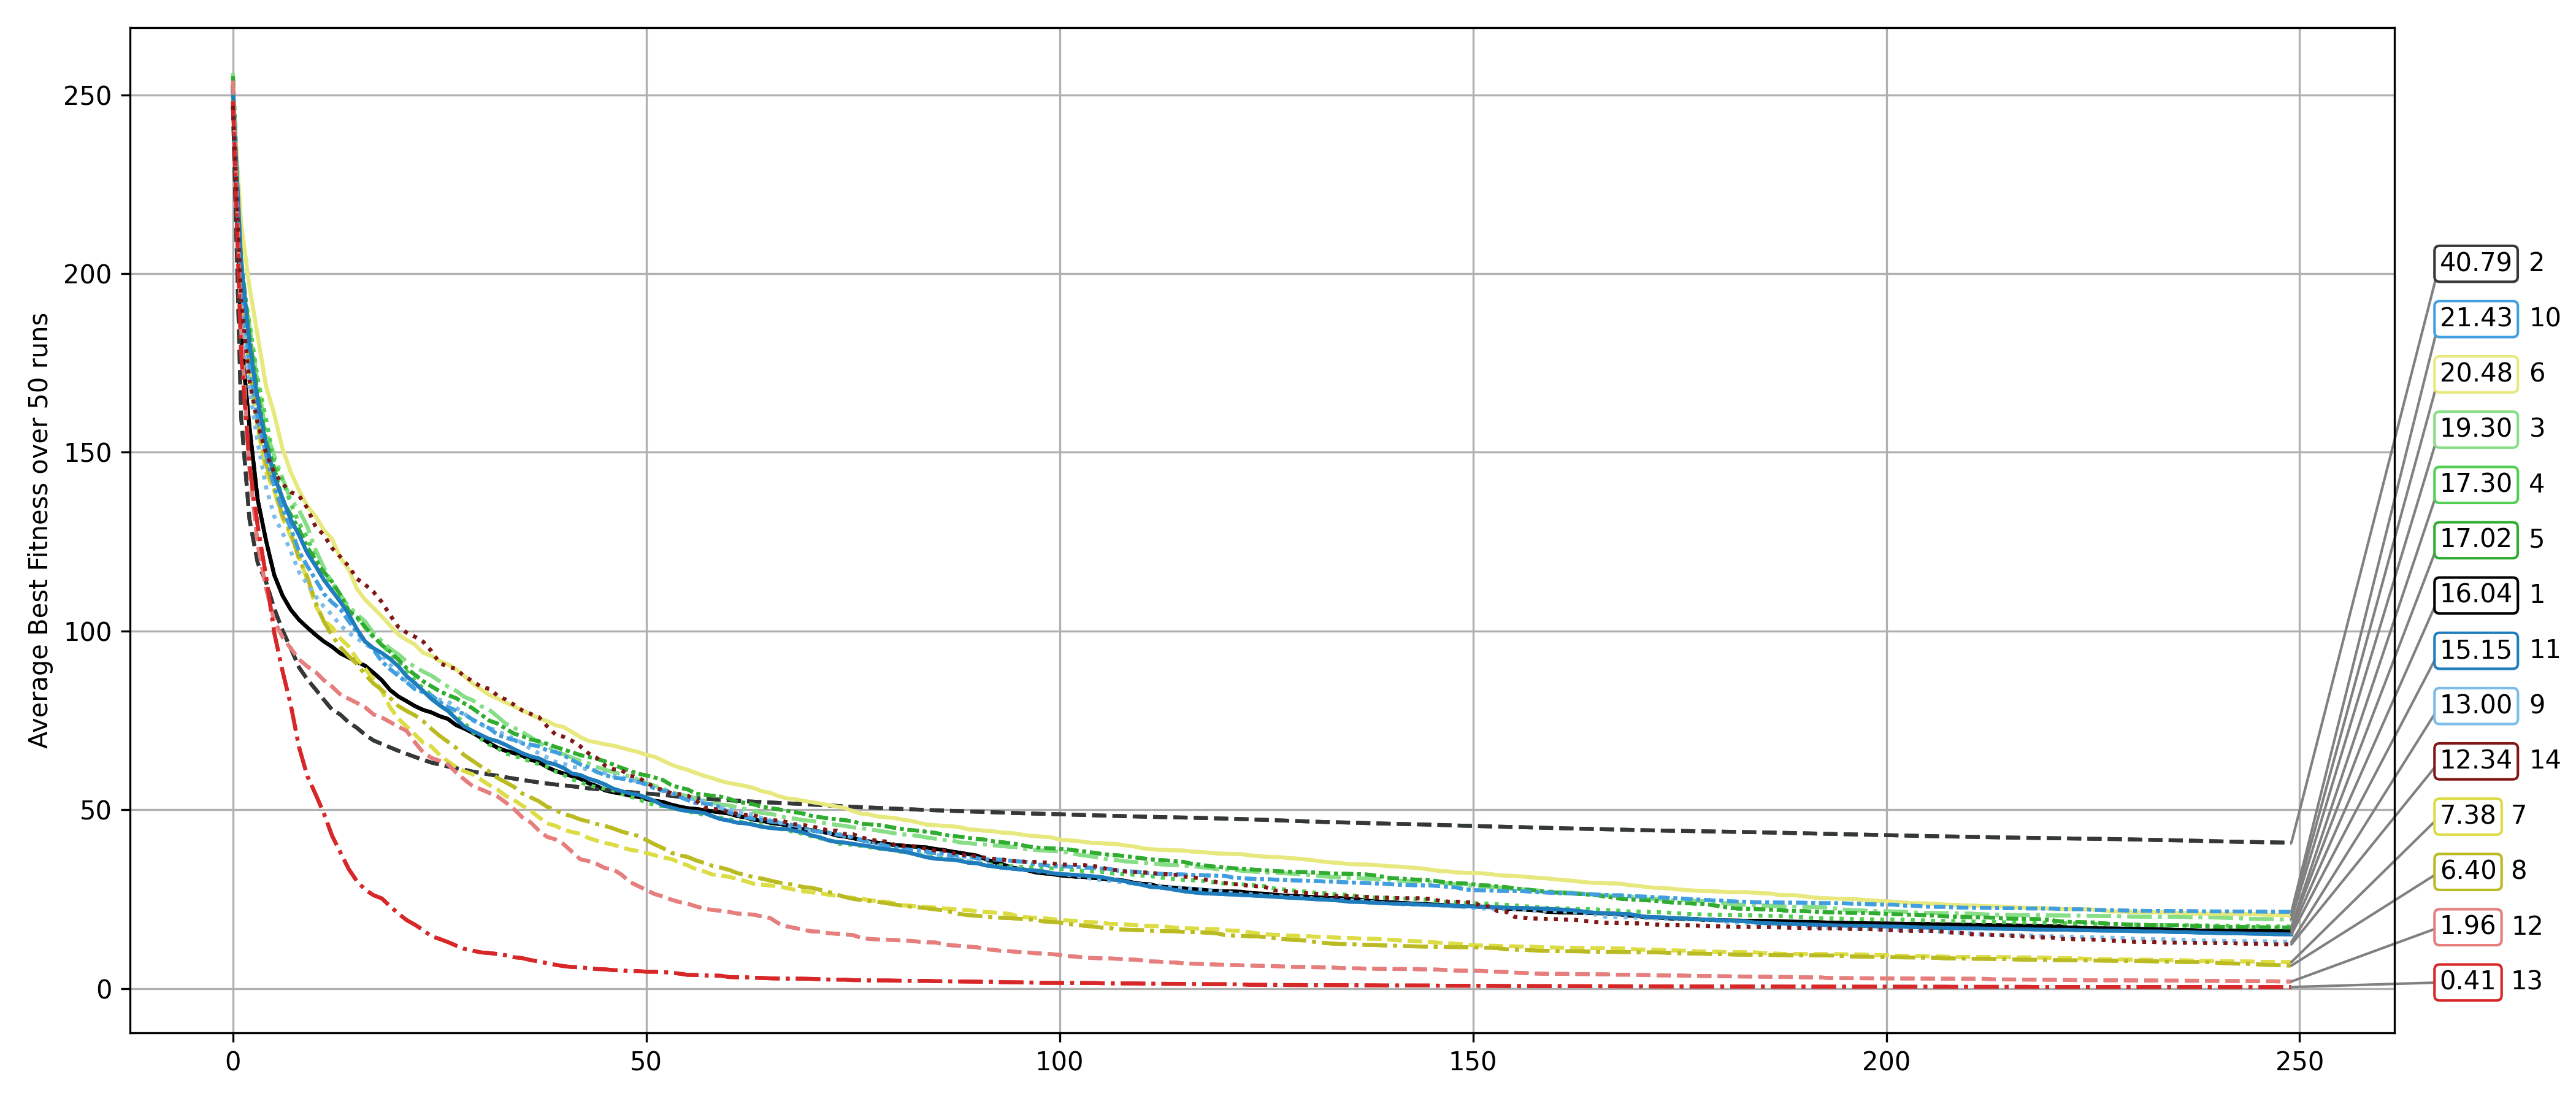
\includegraphics[width=.49\textwidth]{Figures/results/100/Schwefel_N20_All_selected_algorithms_dim100_annot_legend.png}
    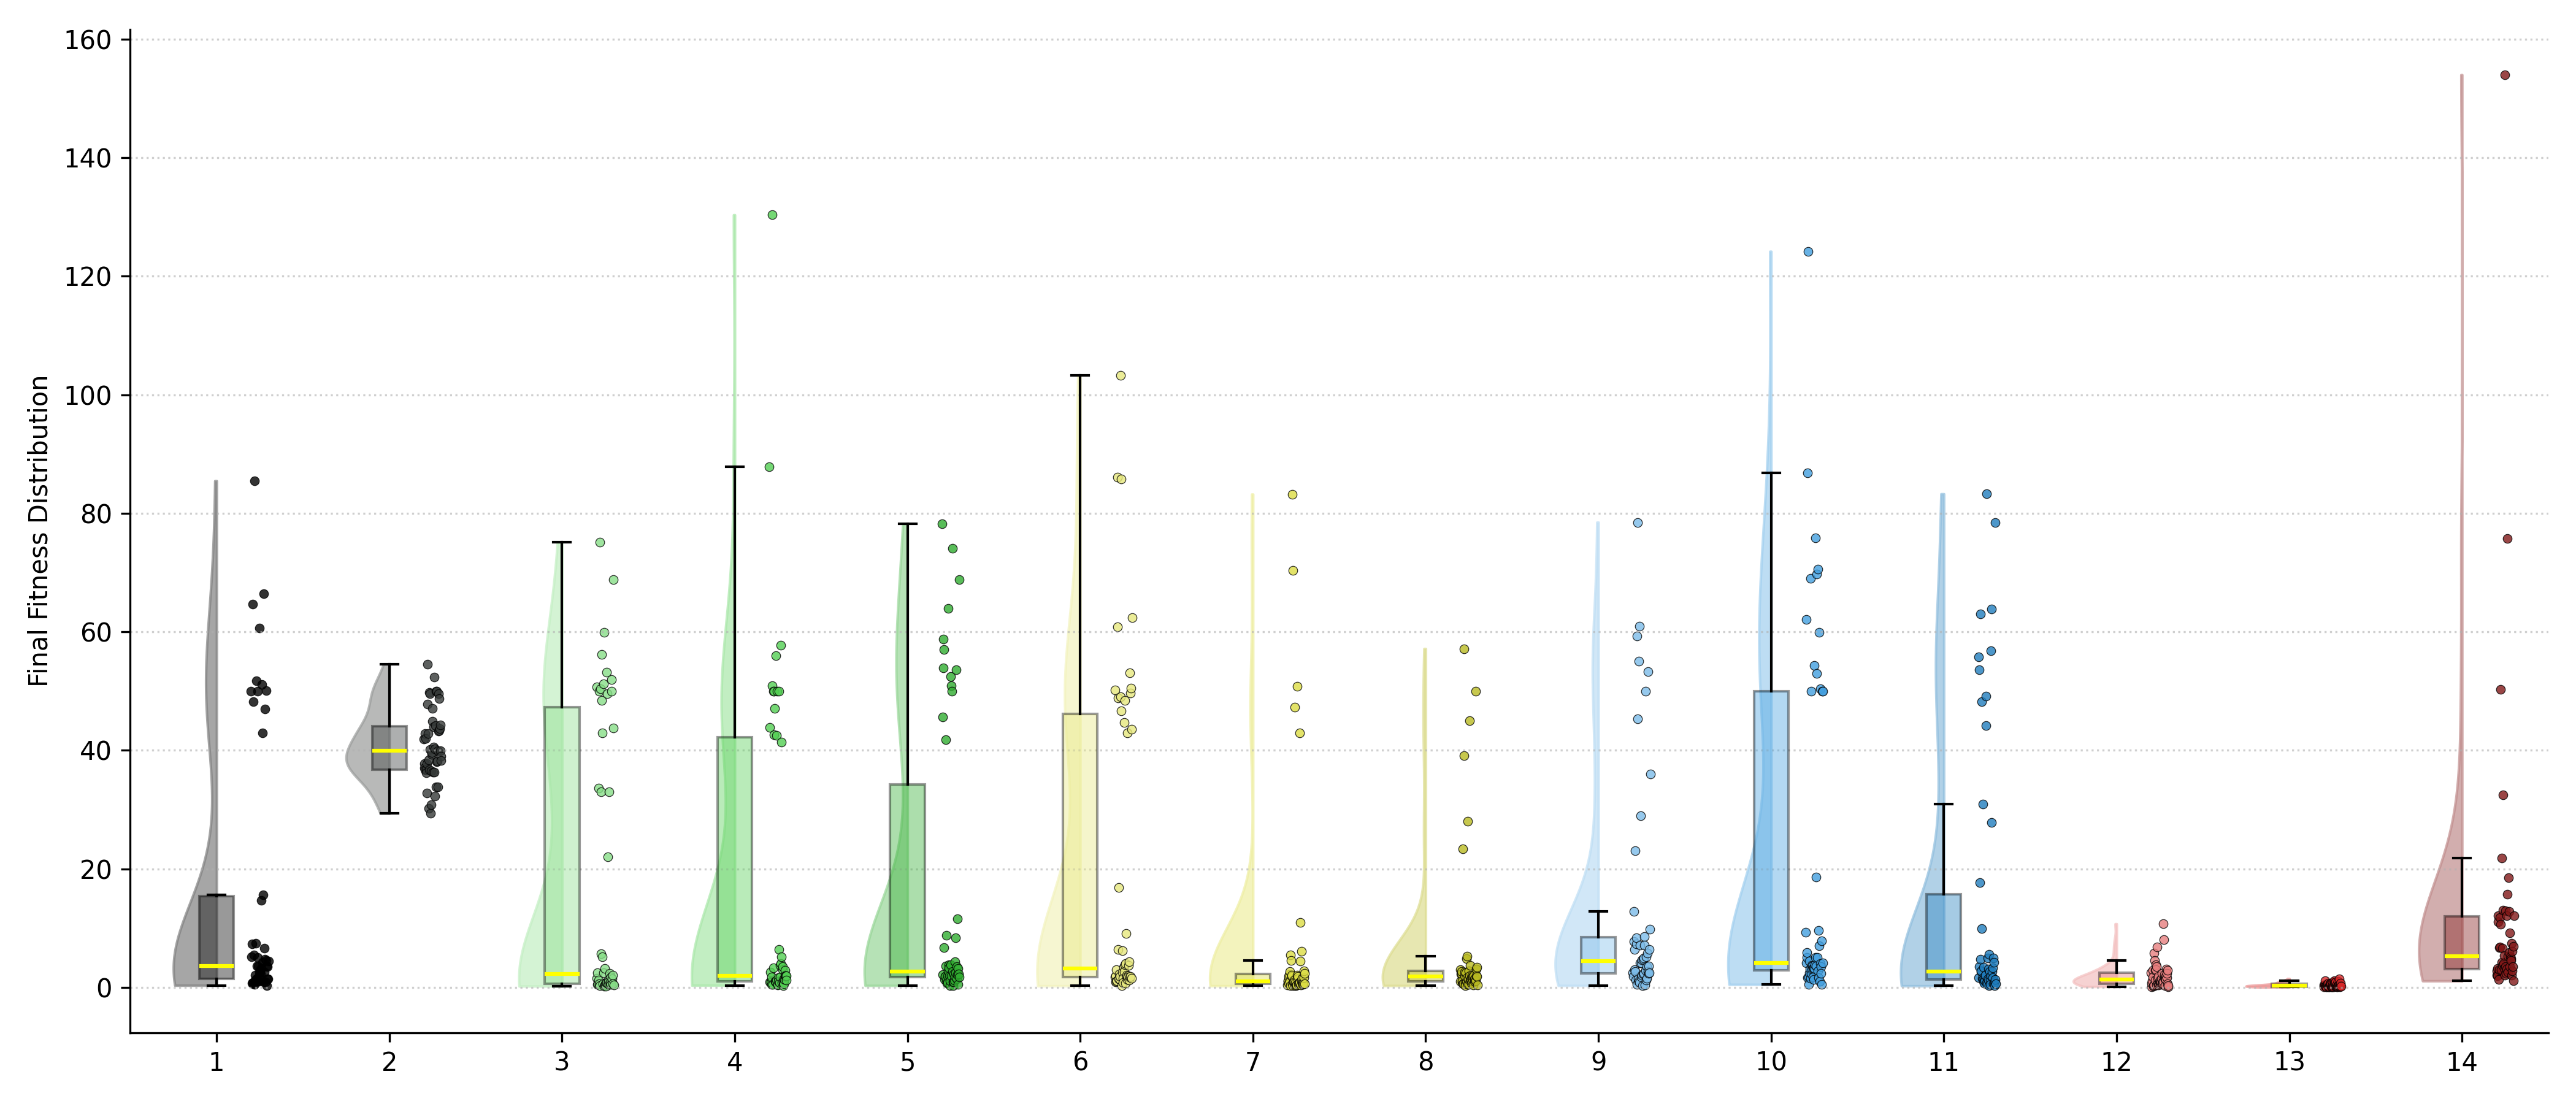
\includegraphics[width=.49\textwidth]{Figures/results/100/Schwefel_N20_all_dim100_raincloud_vertical.png}
    \caption{Schwefel N.20}
\end{subfigure}

\begin{subfigure}{1\textwidth}
    \centering
    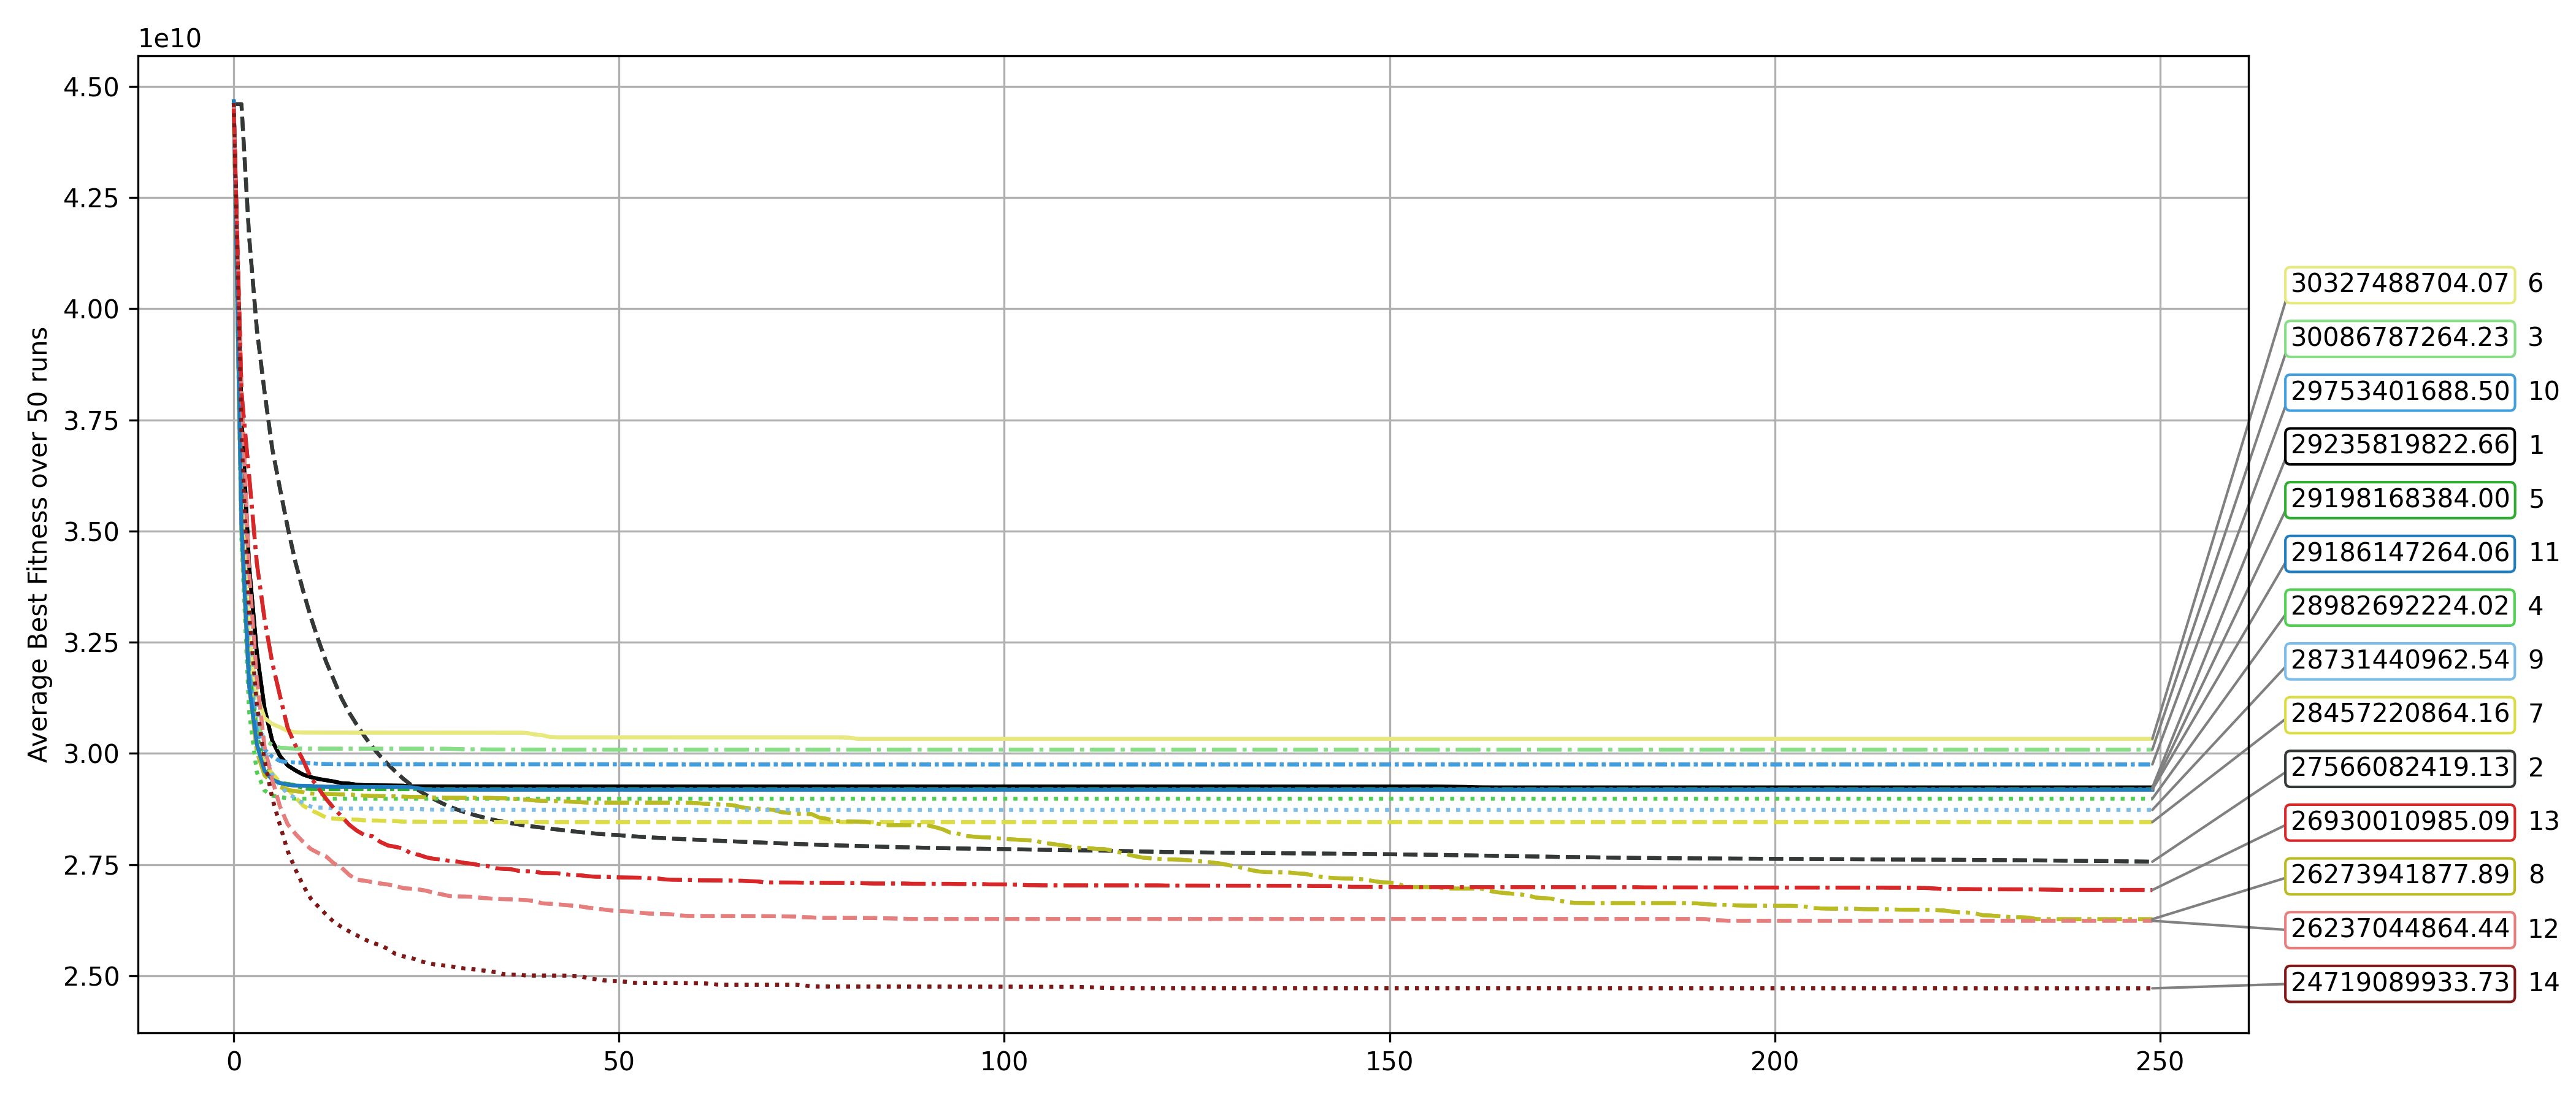
\includegraphics[width=.49\textwidth]{Figures/results/100/Schwefel_N36_All_selected_algorithms_dim100_annot_legend.png}
    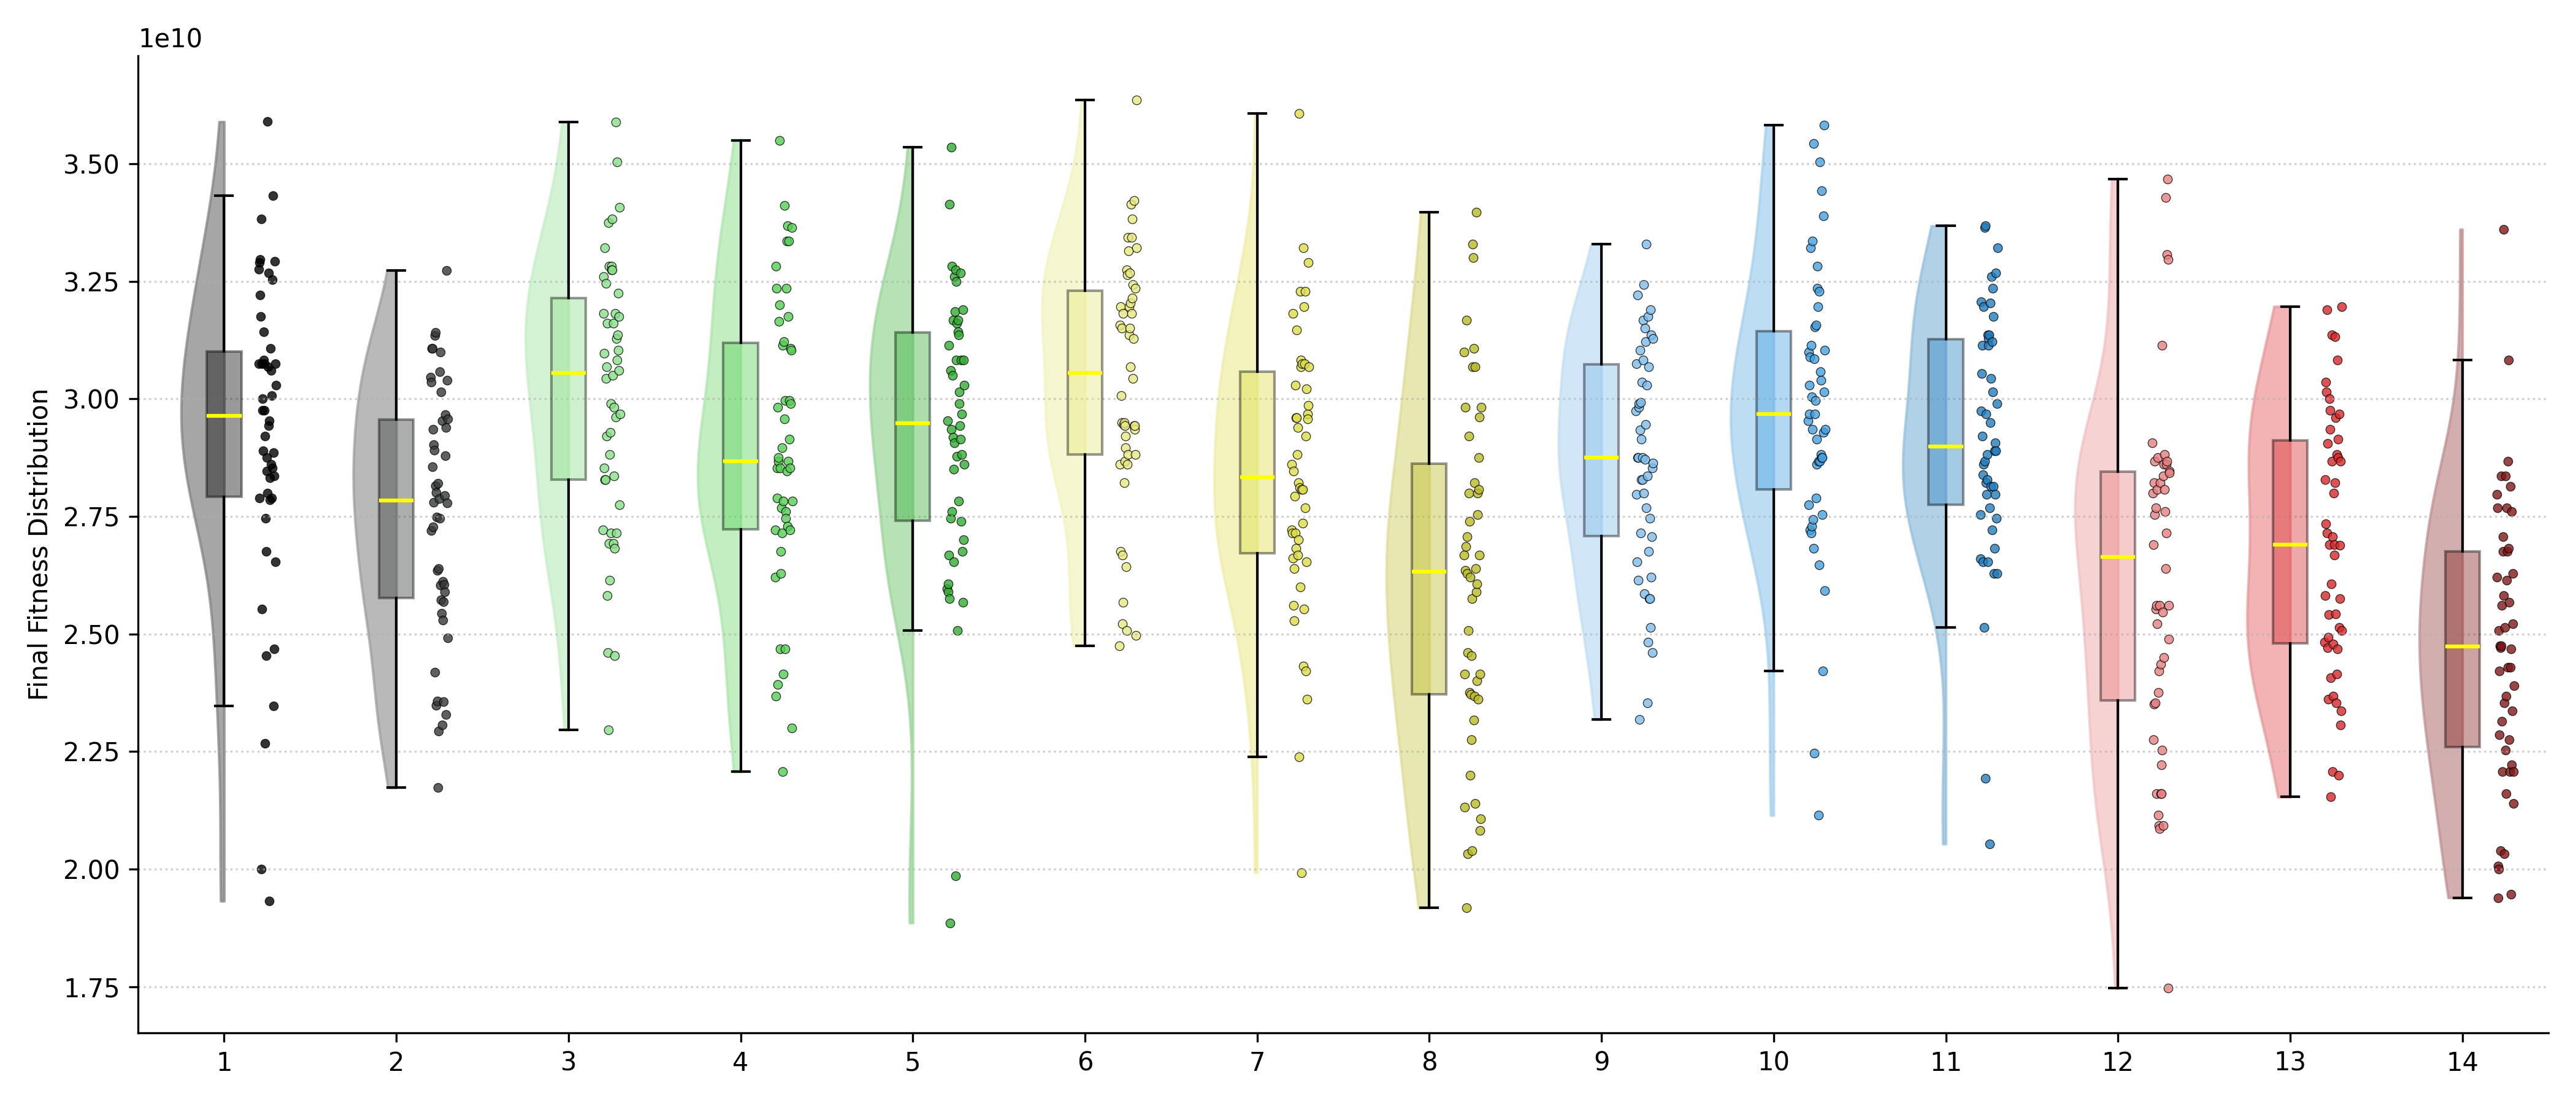
\includegraphics[width=.49\textwidth]{Figures/results/100/Schwefel_N36_all_dim100_raincloud_vertical.png}
    \caption{Schwefel N36}
\end{subfigure}

\begin{subfigure}{1\textwidth}
    \centering
    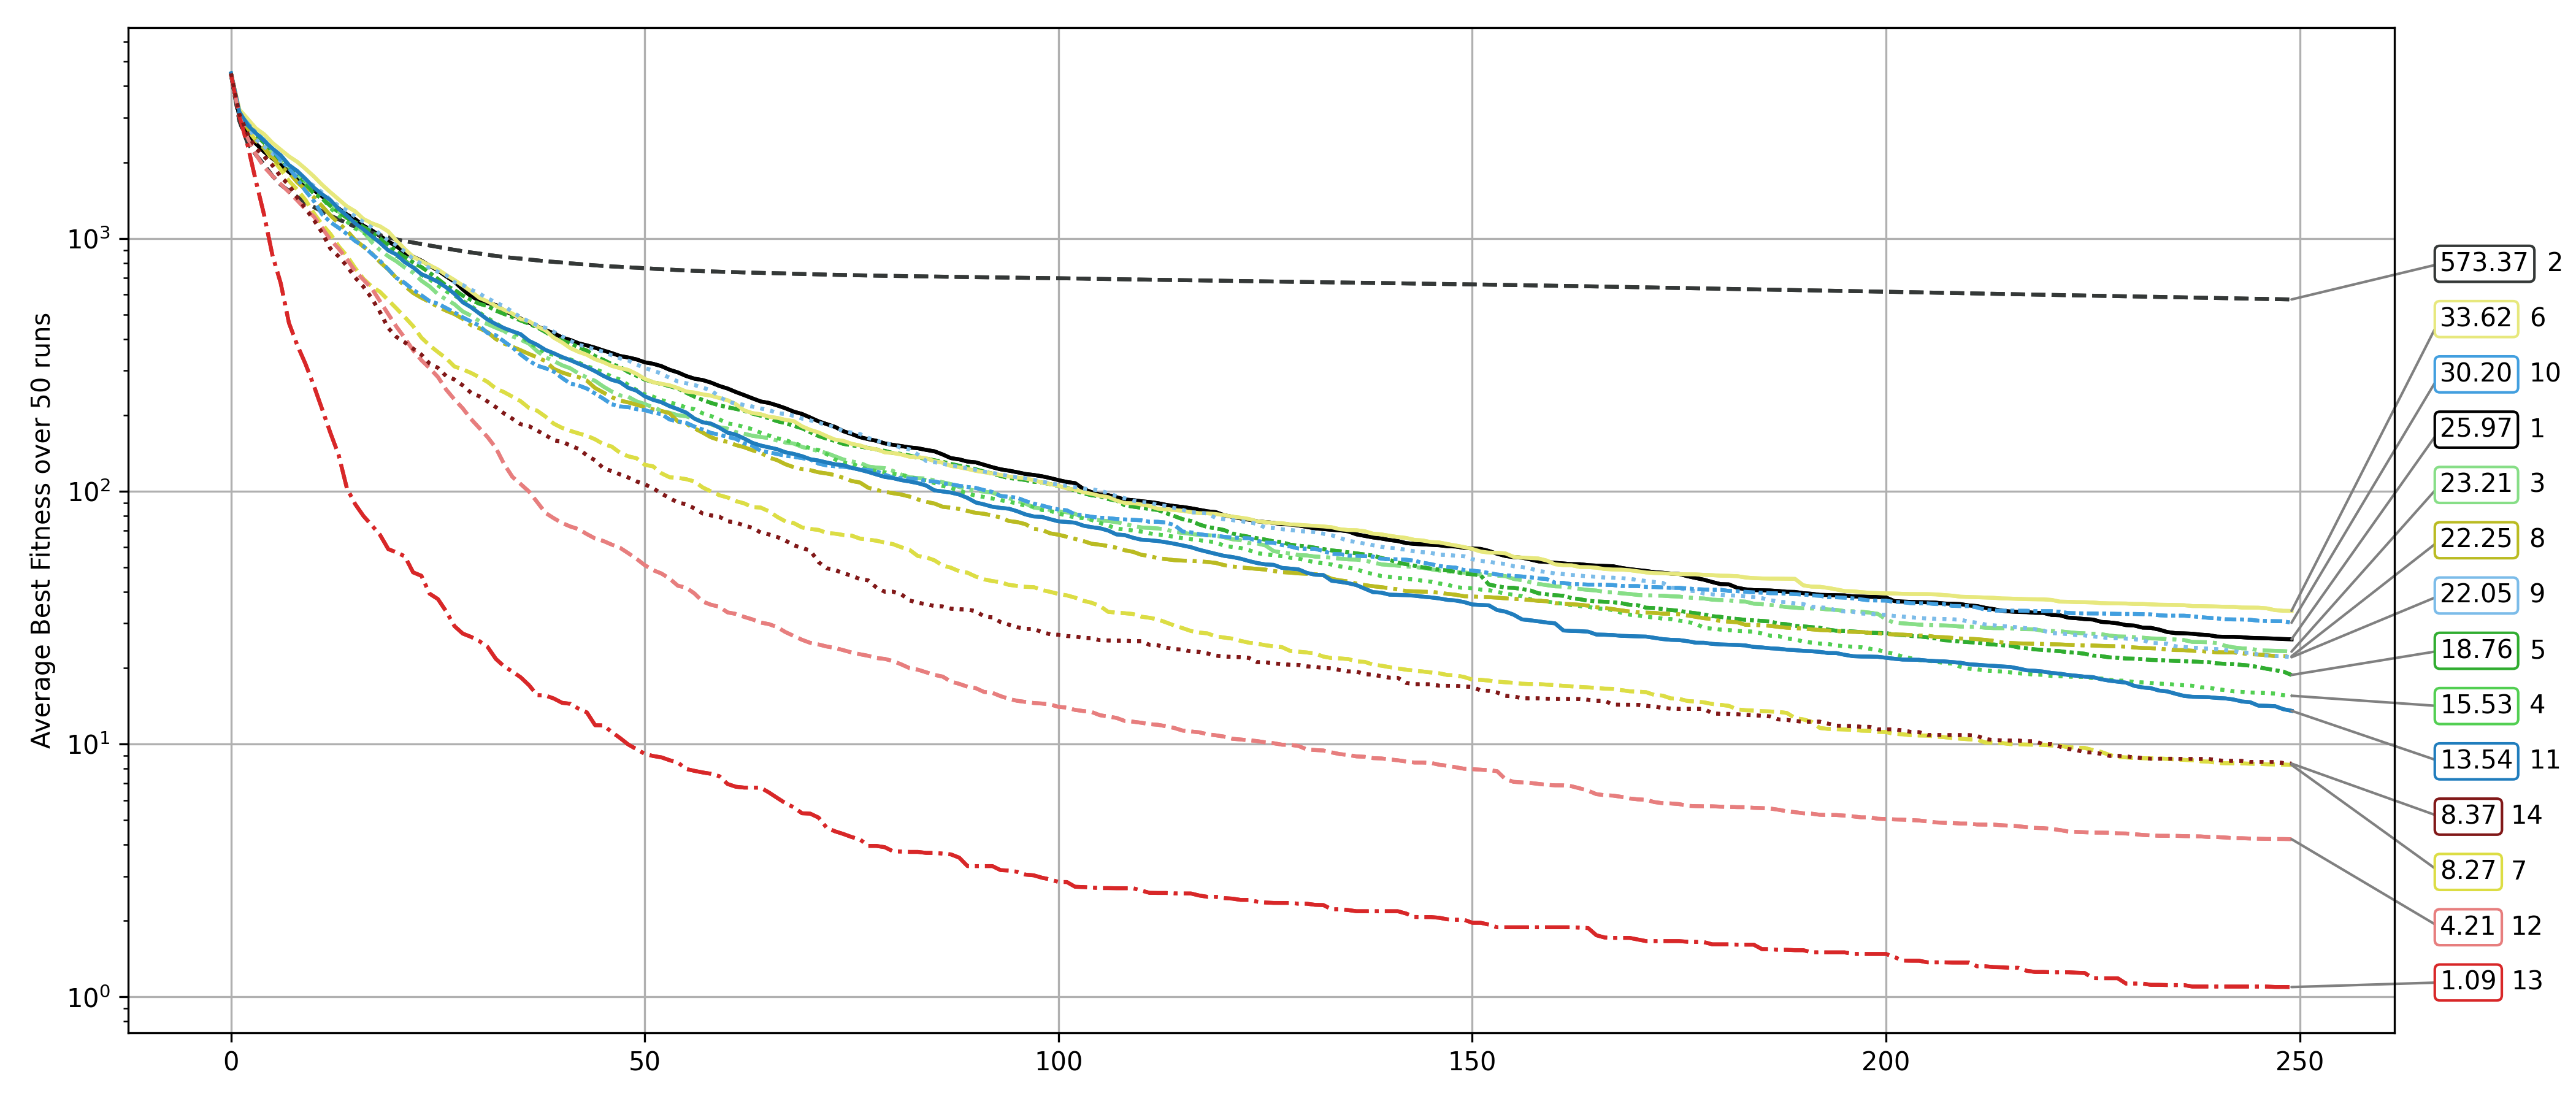
\includegraphics[width=.49\textwidth]{Figures/results/100/Schwefel_N6_All_selected_algorithms_dim100_annot_legend.png}
    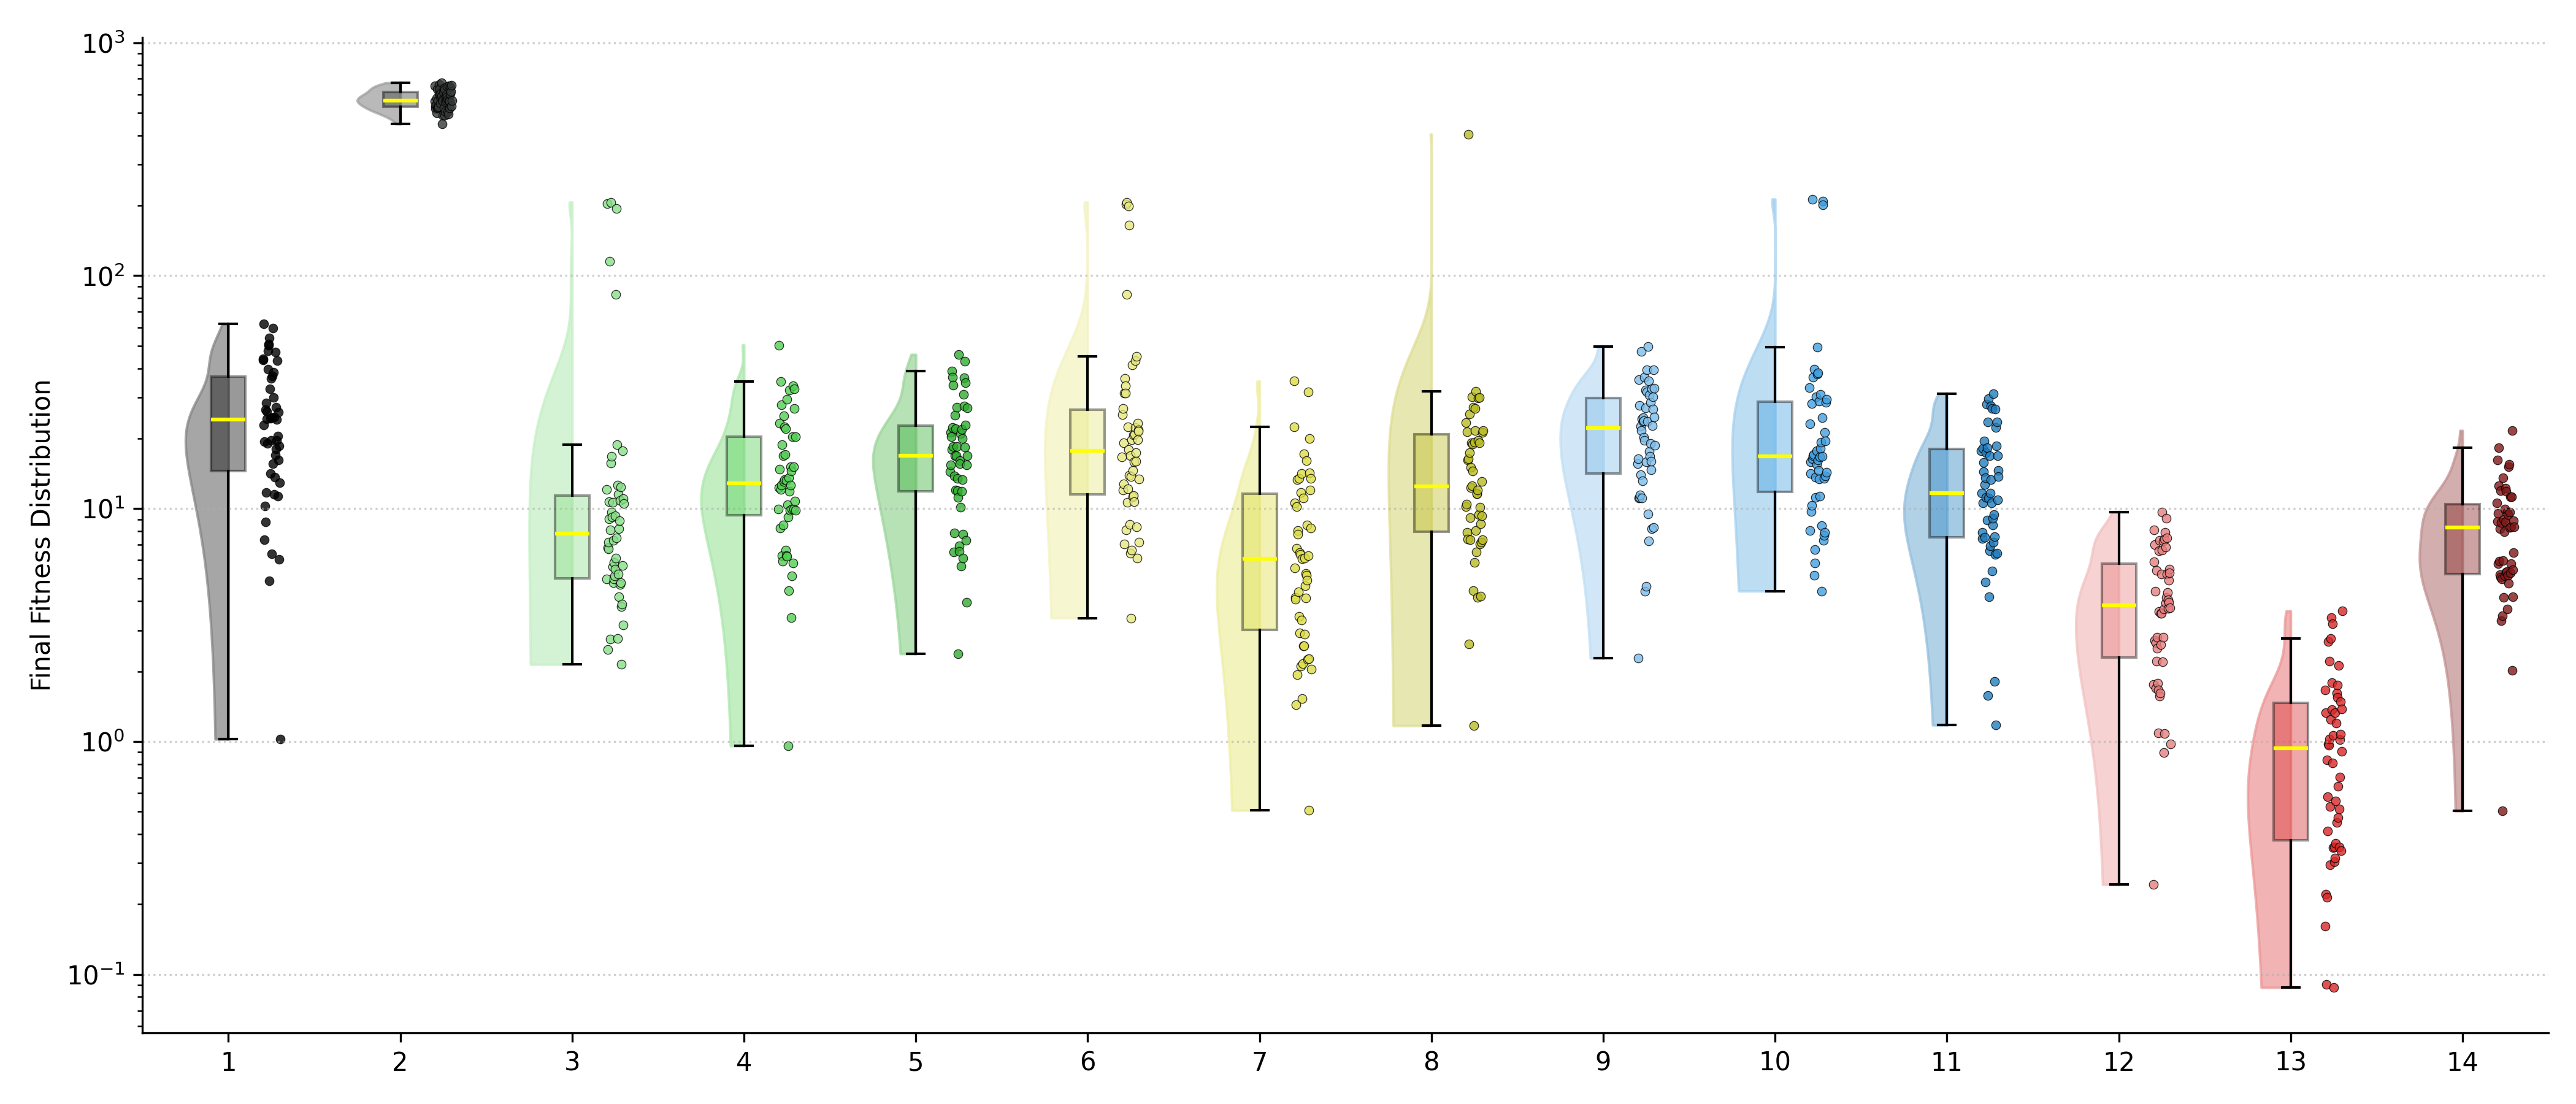
\includegraphics[width=.49\textwidth]{Figures/results/100/Schwefel_N6_all_dim100_raincloud_vertical.png}
    \caption{Schwefel N6 (log)}
\end{subfigure}

\begin{subfigure}{1\textwidth}
    \centering
    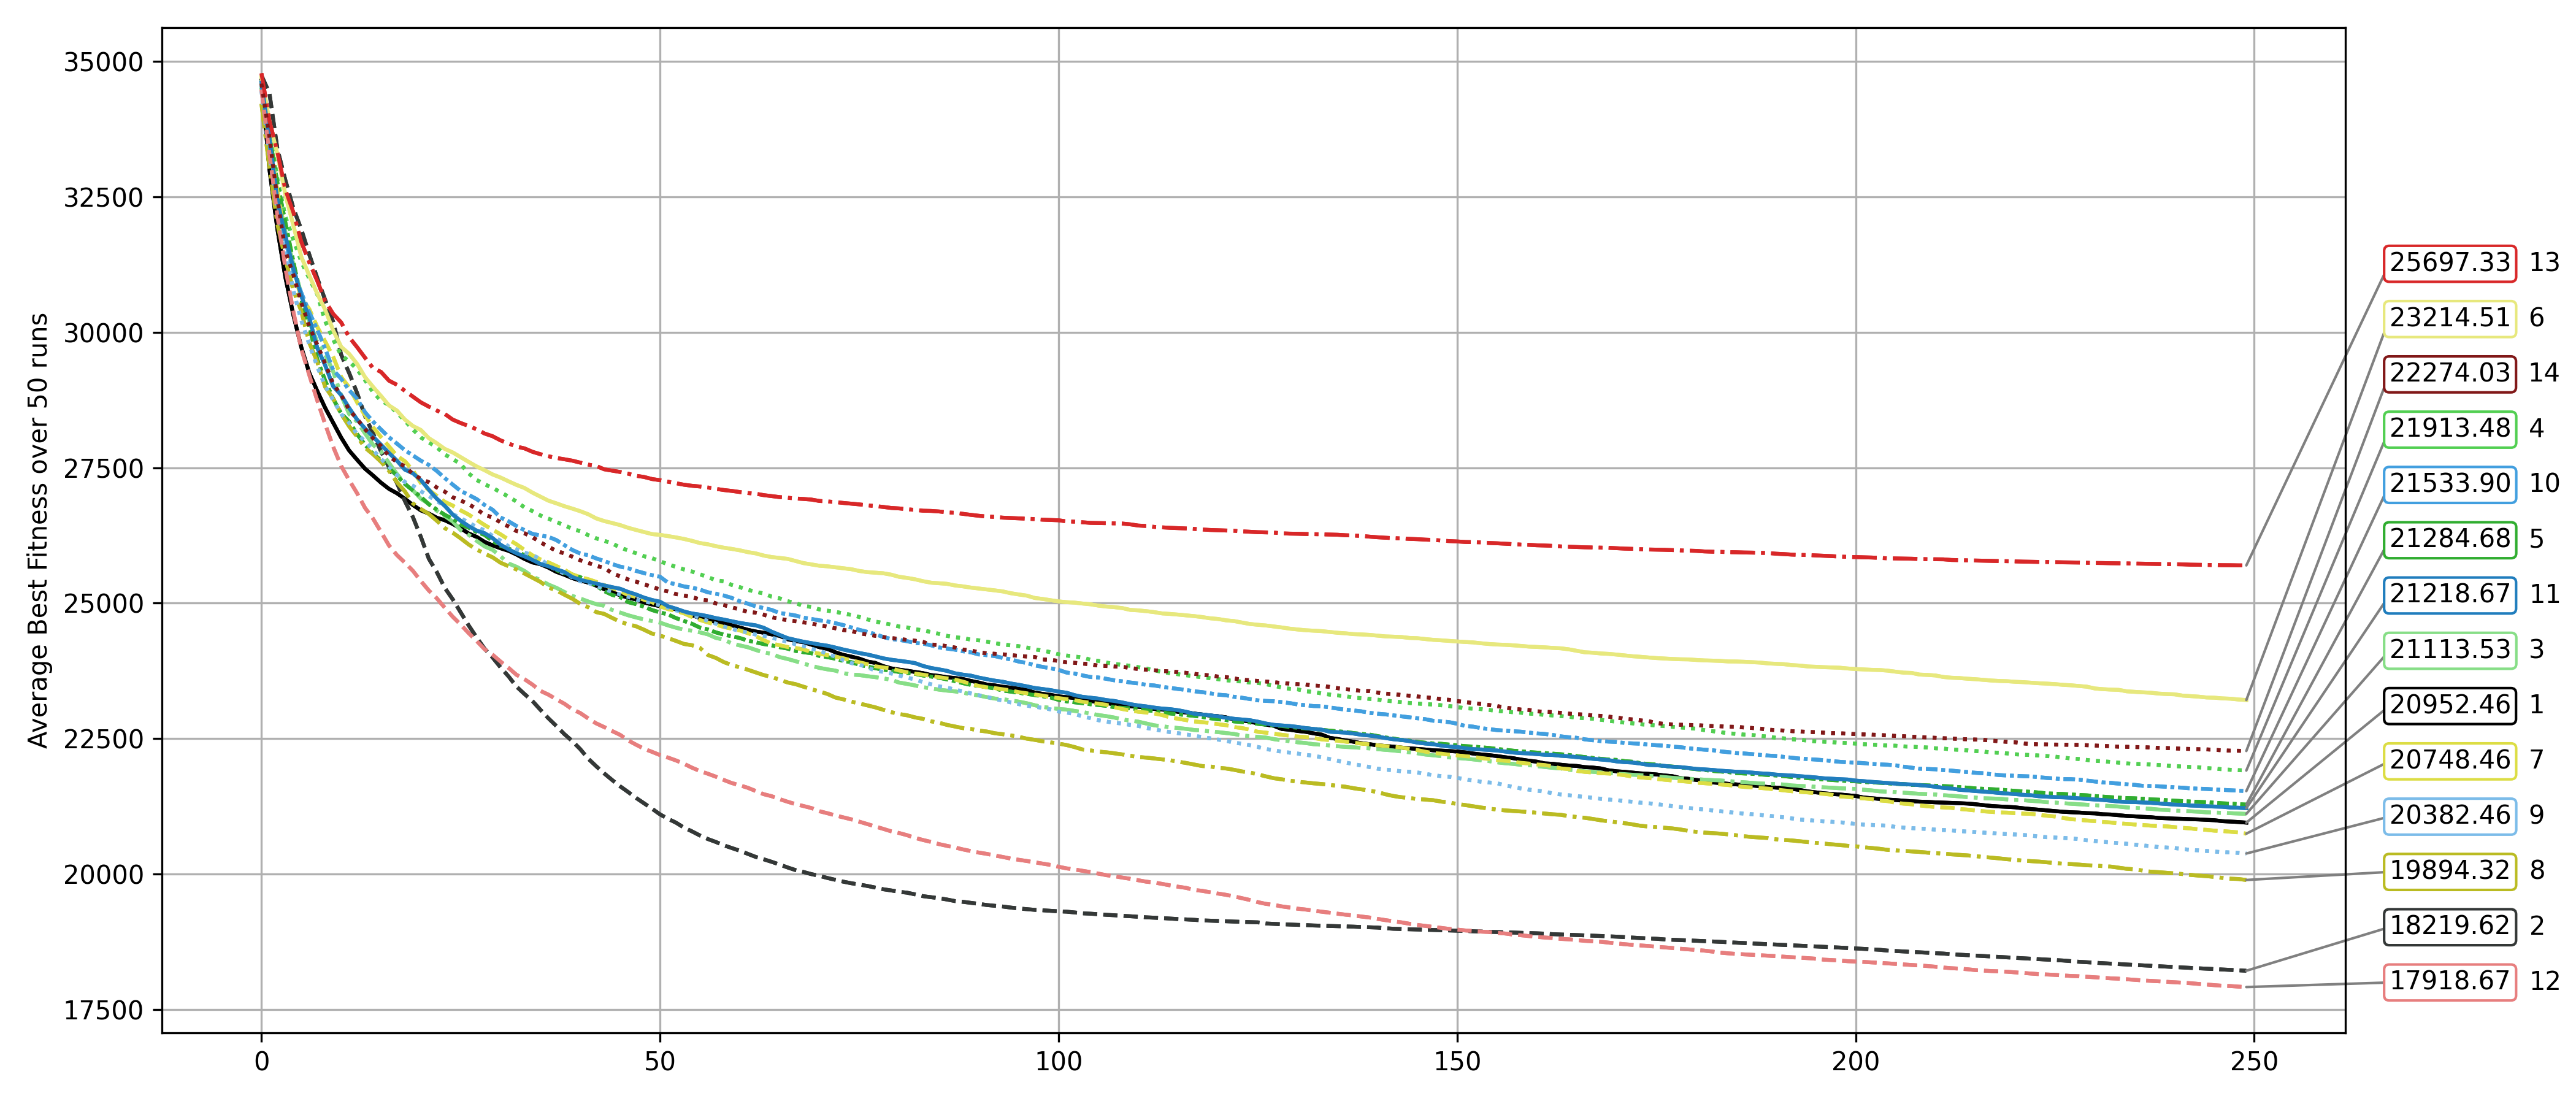
\includegraphics[width=.49\textwidth]{Figures/results/100/Shifted_Schwefel_All_selected_algorithms_dim100_annot_legend.png}
    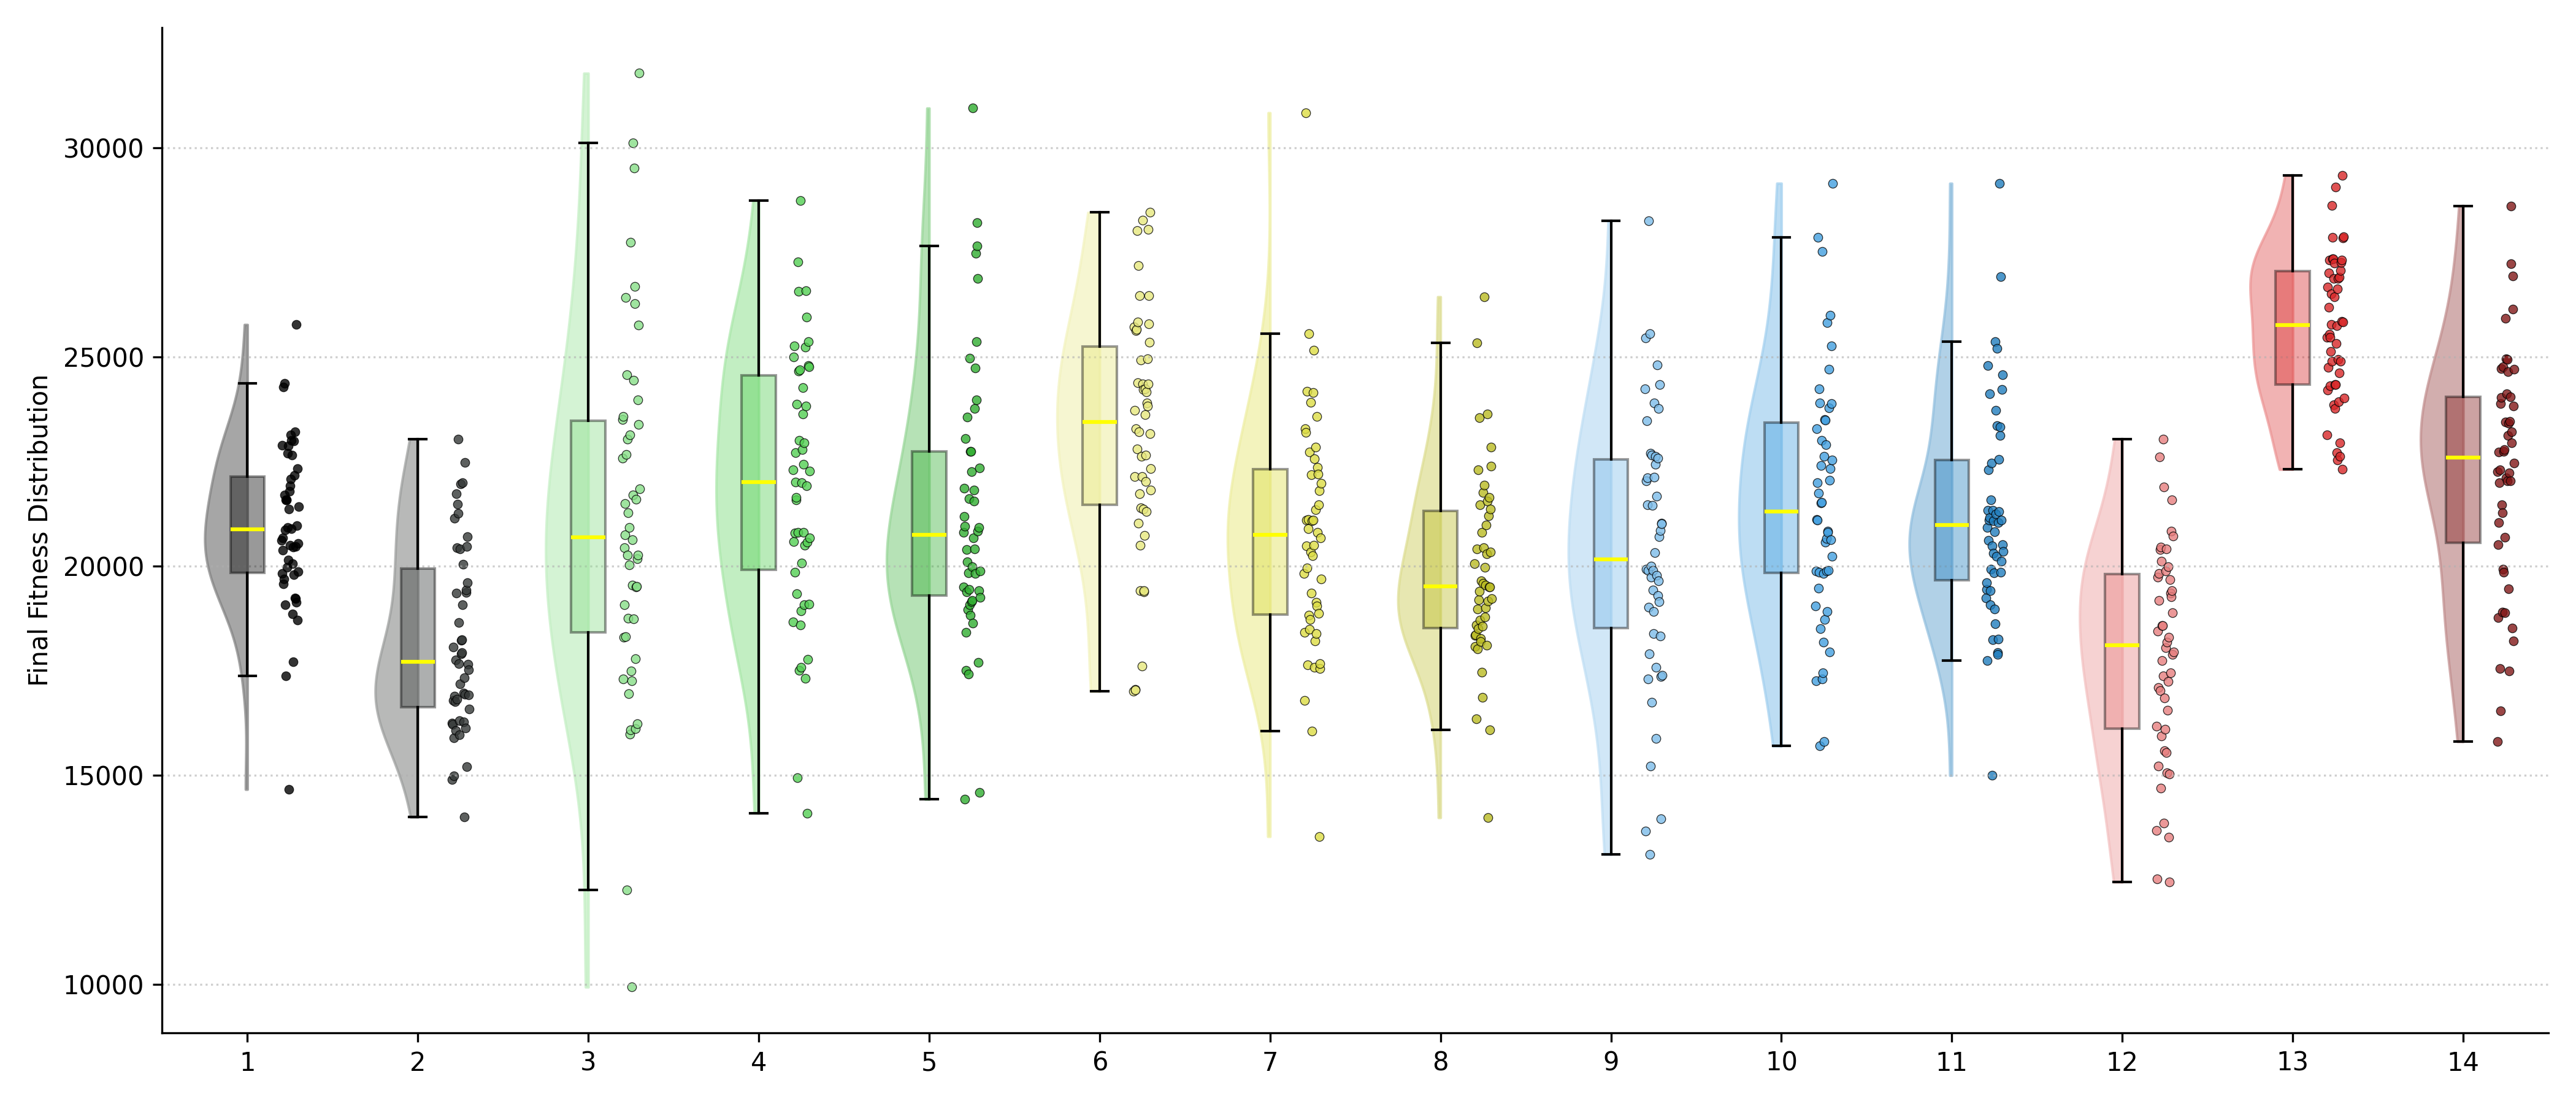
\includegraphics[width=.49\textwidth]{Figures/results/100/Shifted_Schwefel_all_dim100_raincloud_vertical.png}
    \caption{Shifted Schwefel}
\end{subfigure}

\begin{subfigure}{1\textwidth}
    \centering
    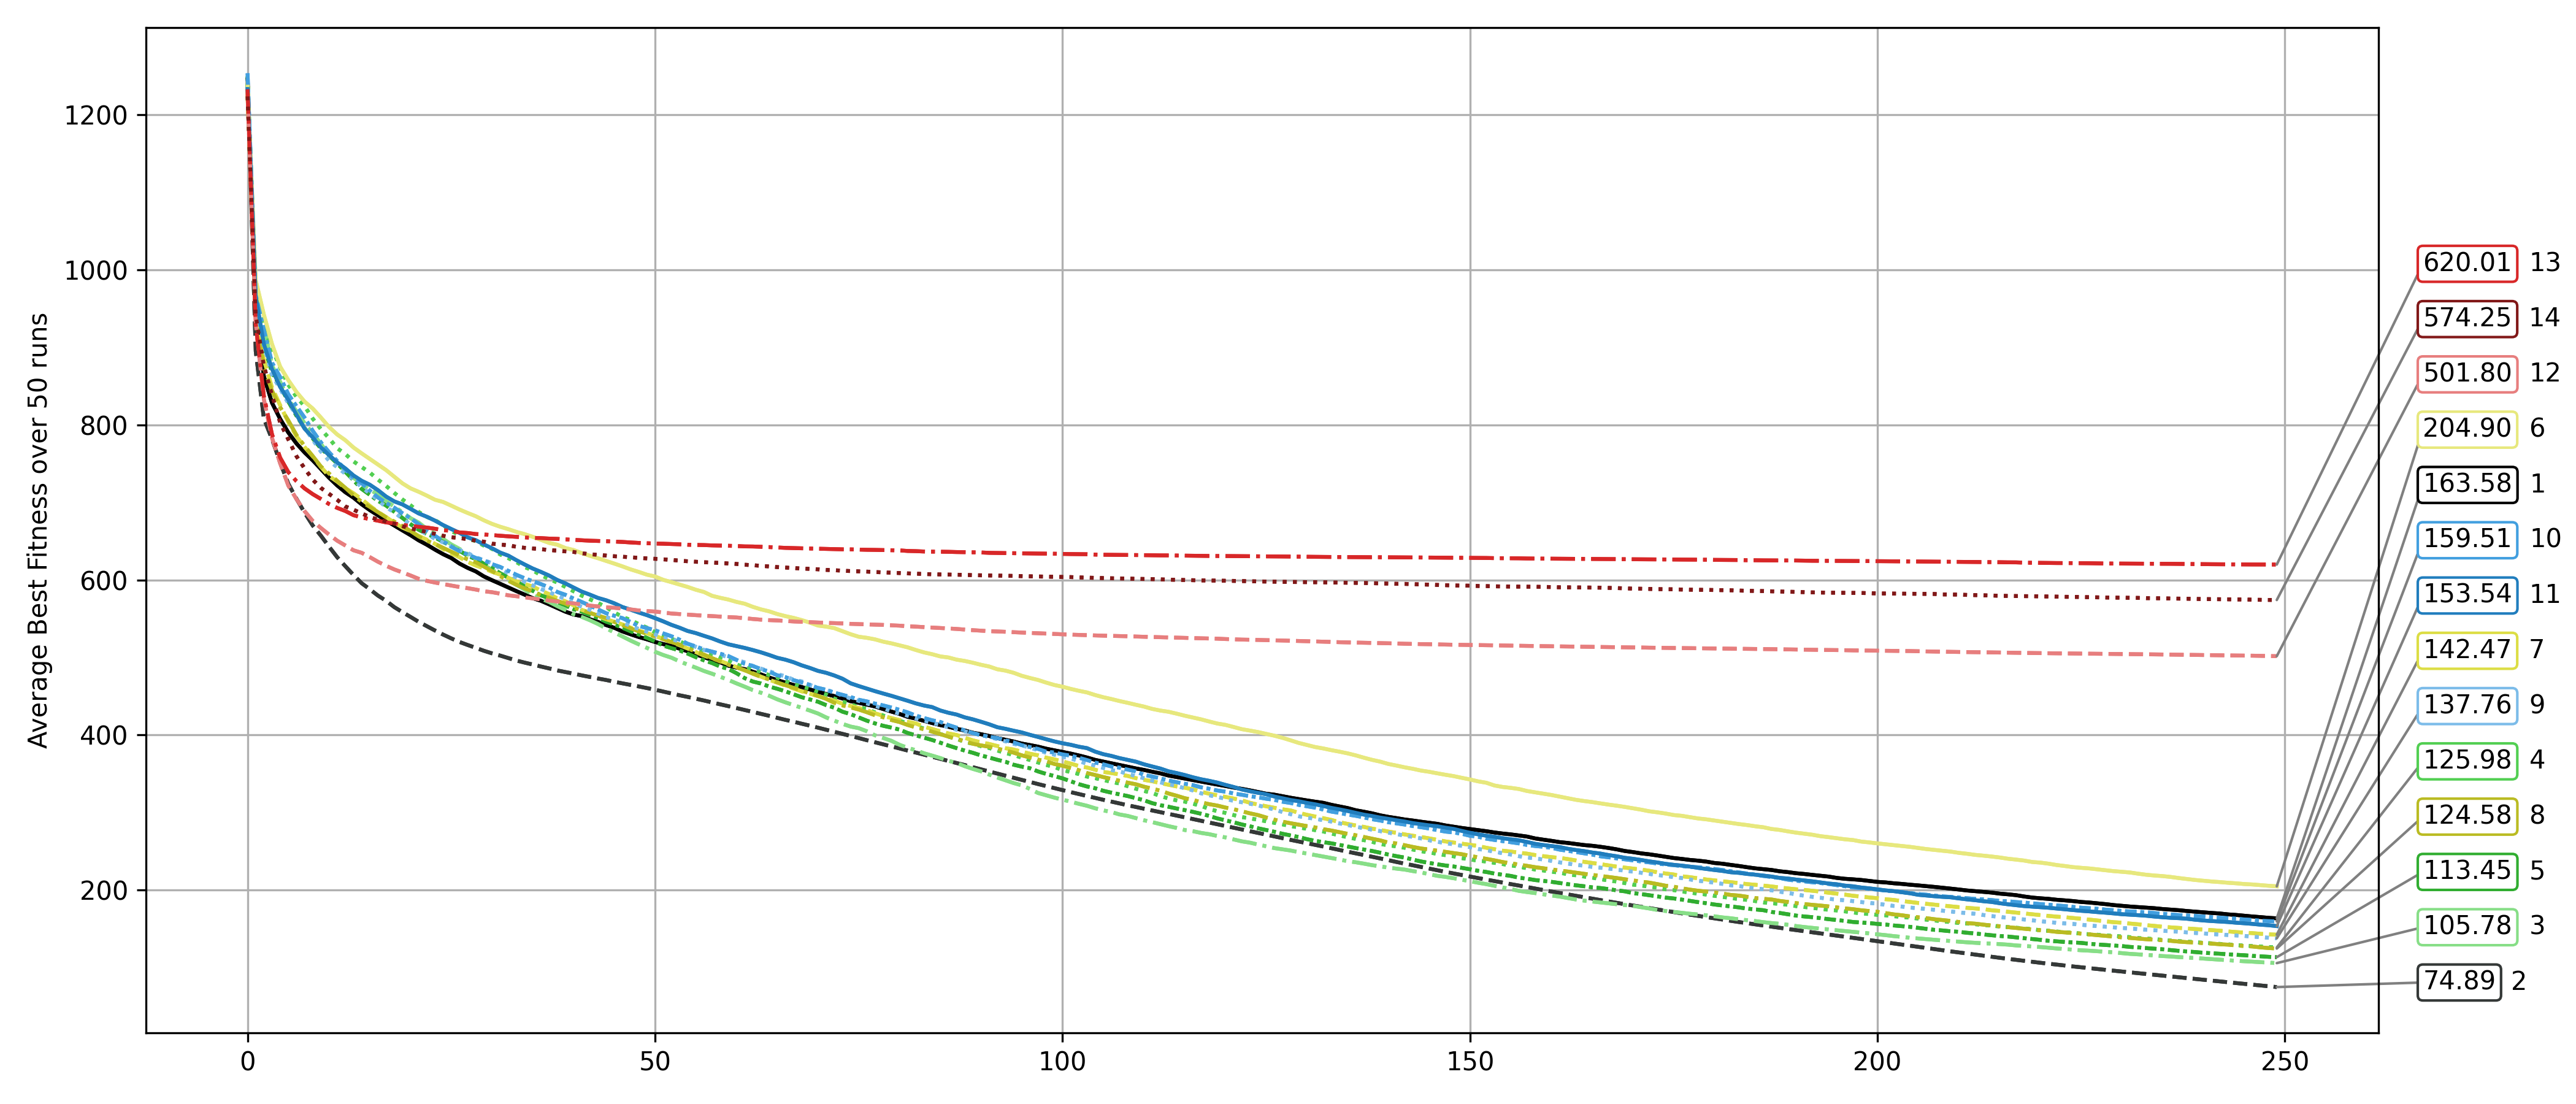
\includegraphics[width=.49\textwidth]{Figures/results/100/Shifted_and_Rotated_HGBat_All_selected_algorithms_dim100_annot_legend.png}
    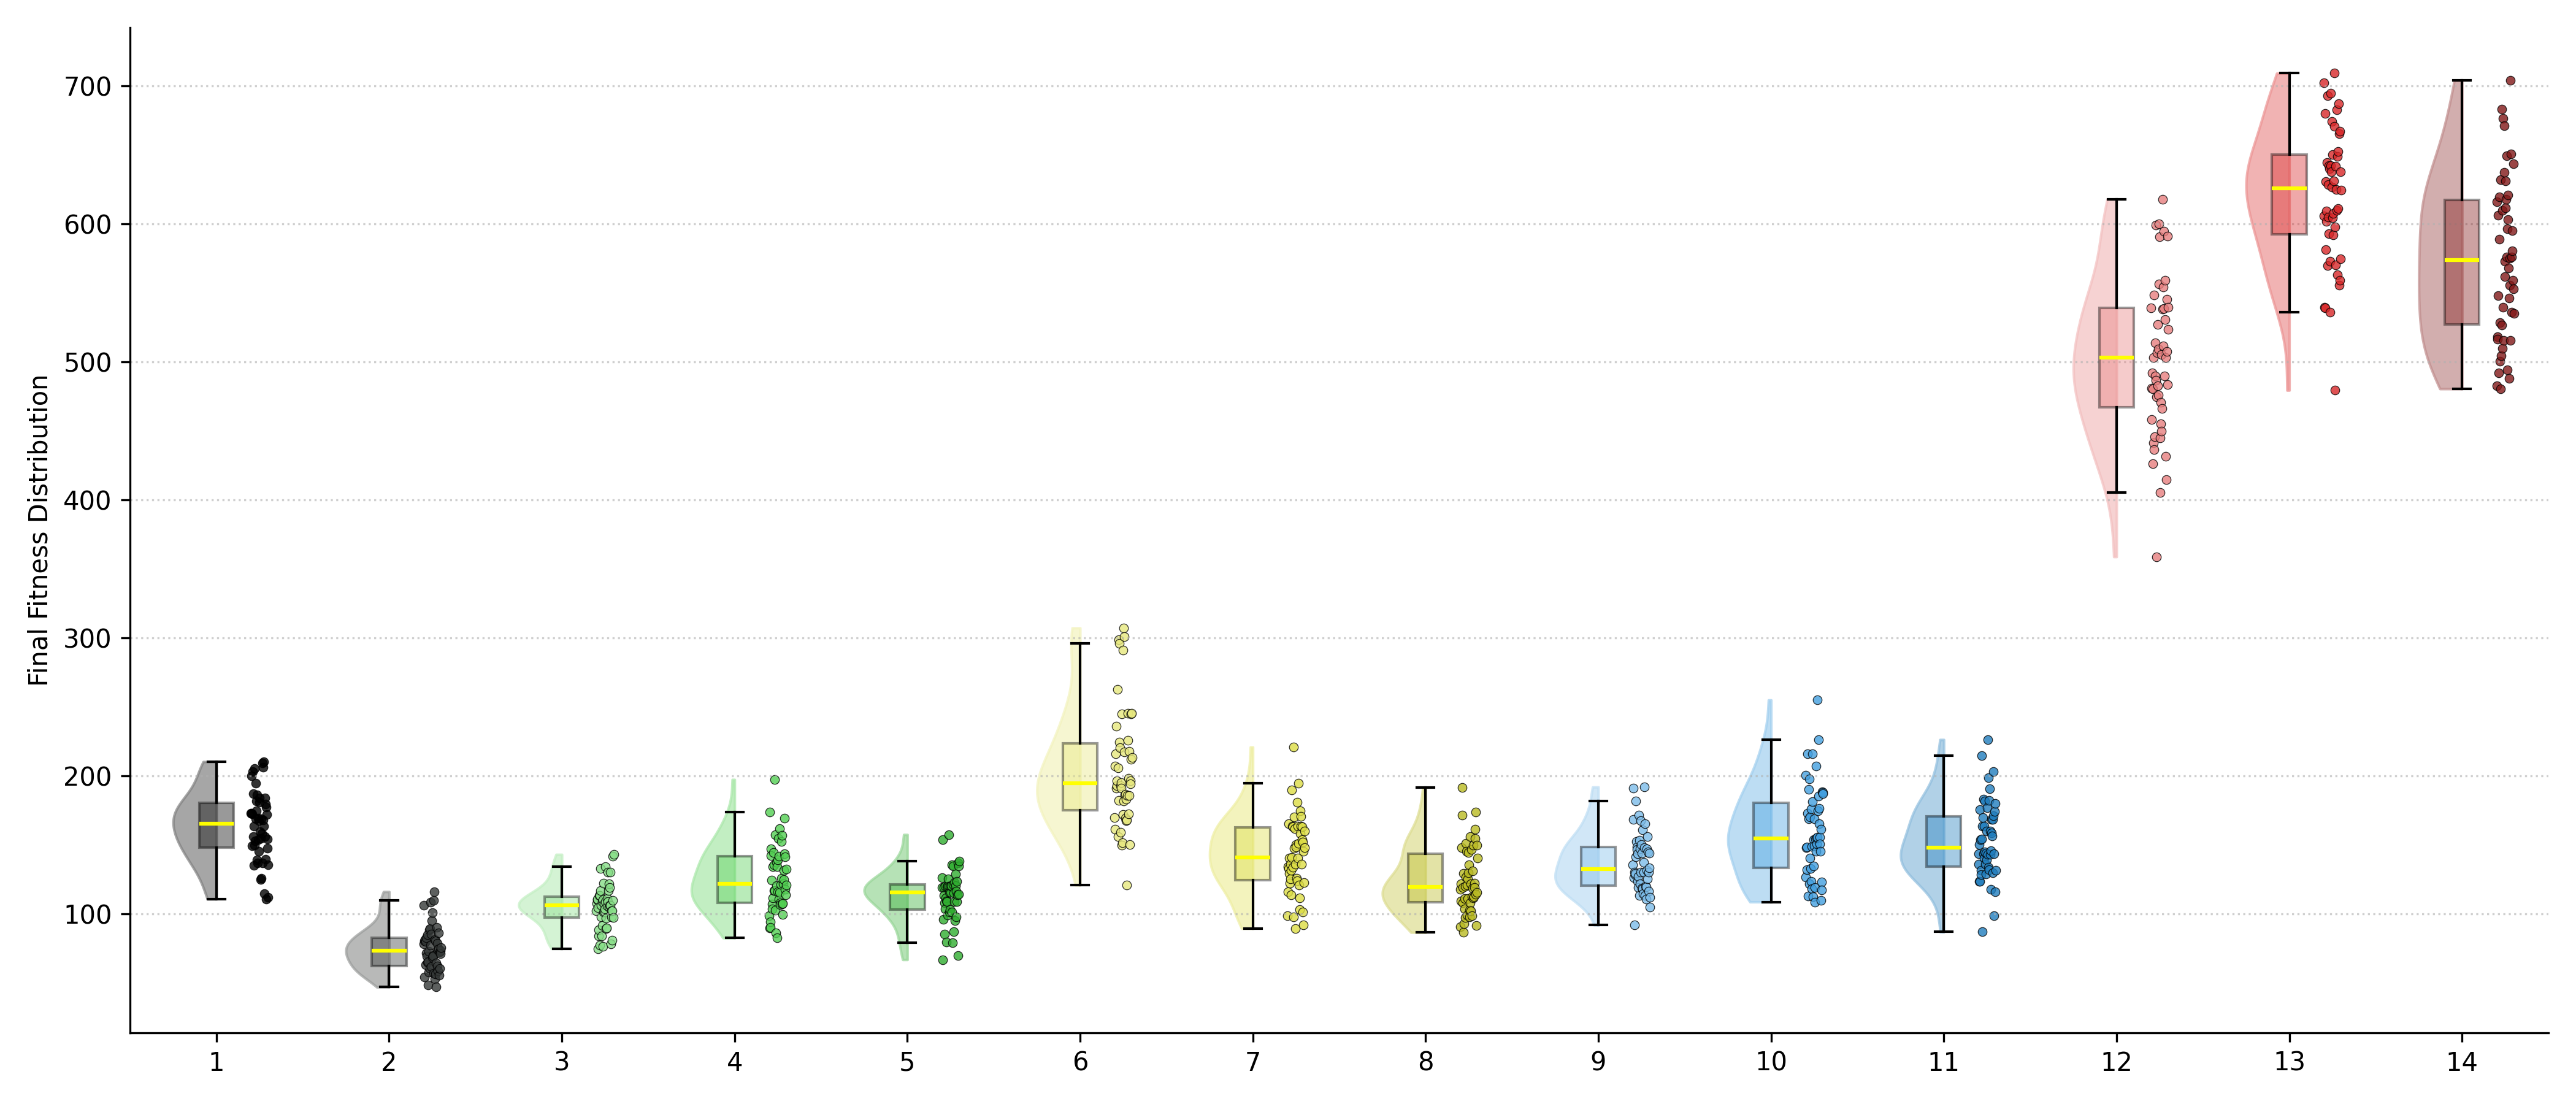
\includegraphics[width=.49\textwidth]{Figures/results/100/Shifted_and_Rotated_HGBat_all_dim100_raincloud_vertical.png}
    \caption{Shifted and Rotated HGBat}
\end{subfigure}

\begin{subfigure}{1\textwidth}
    \centering
    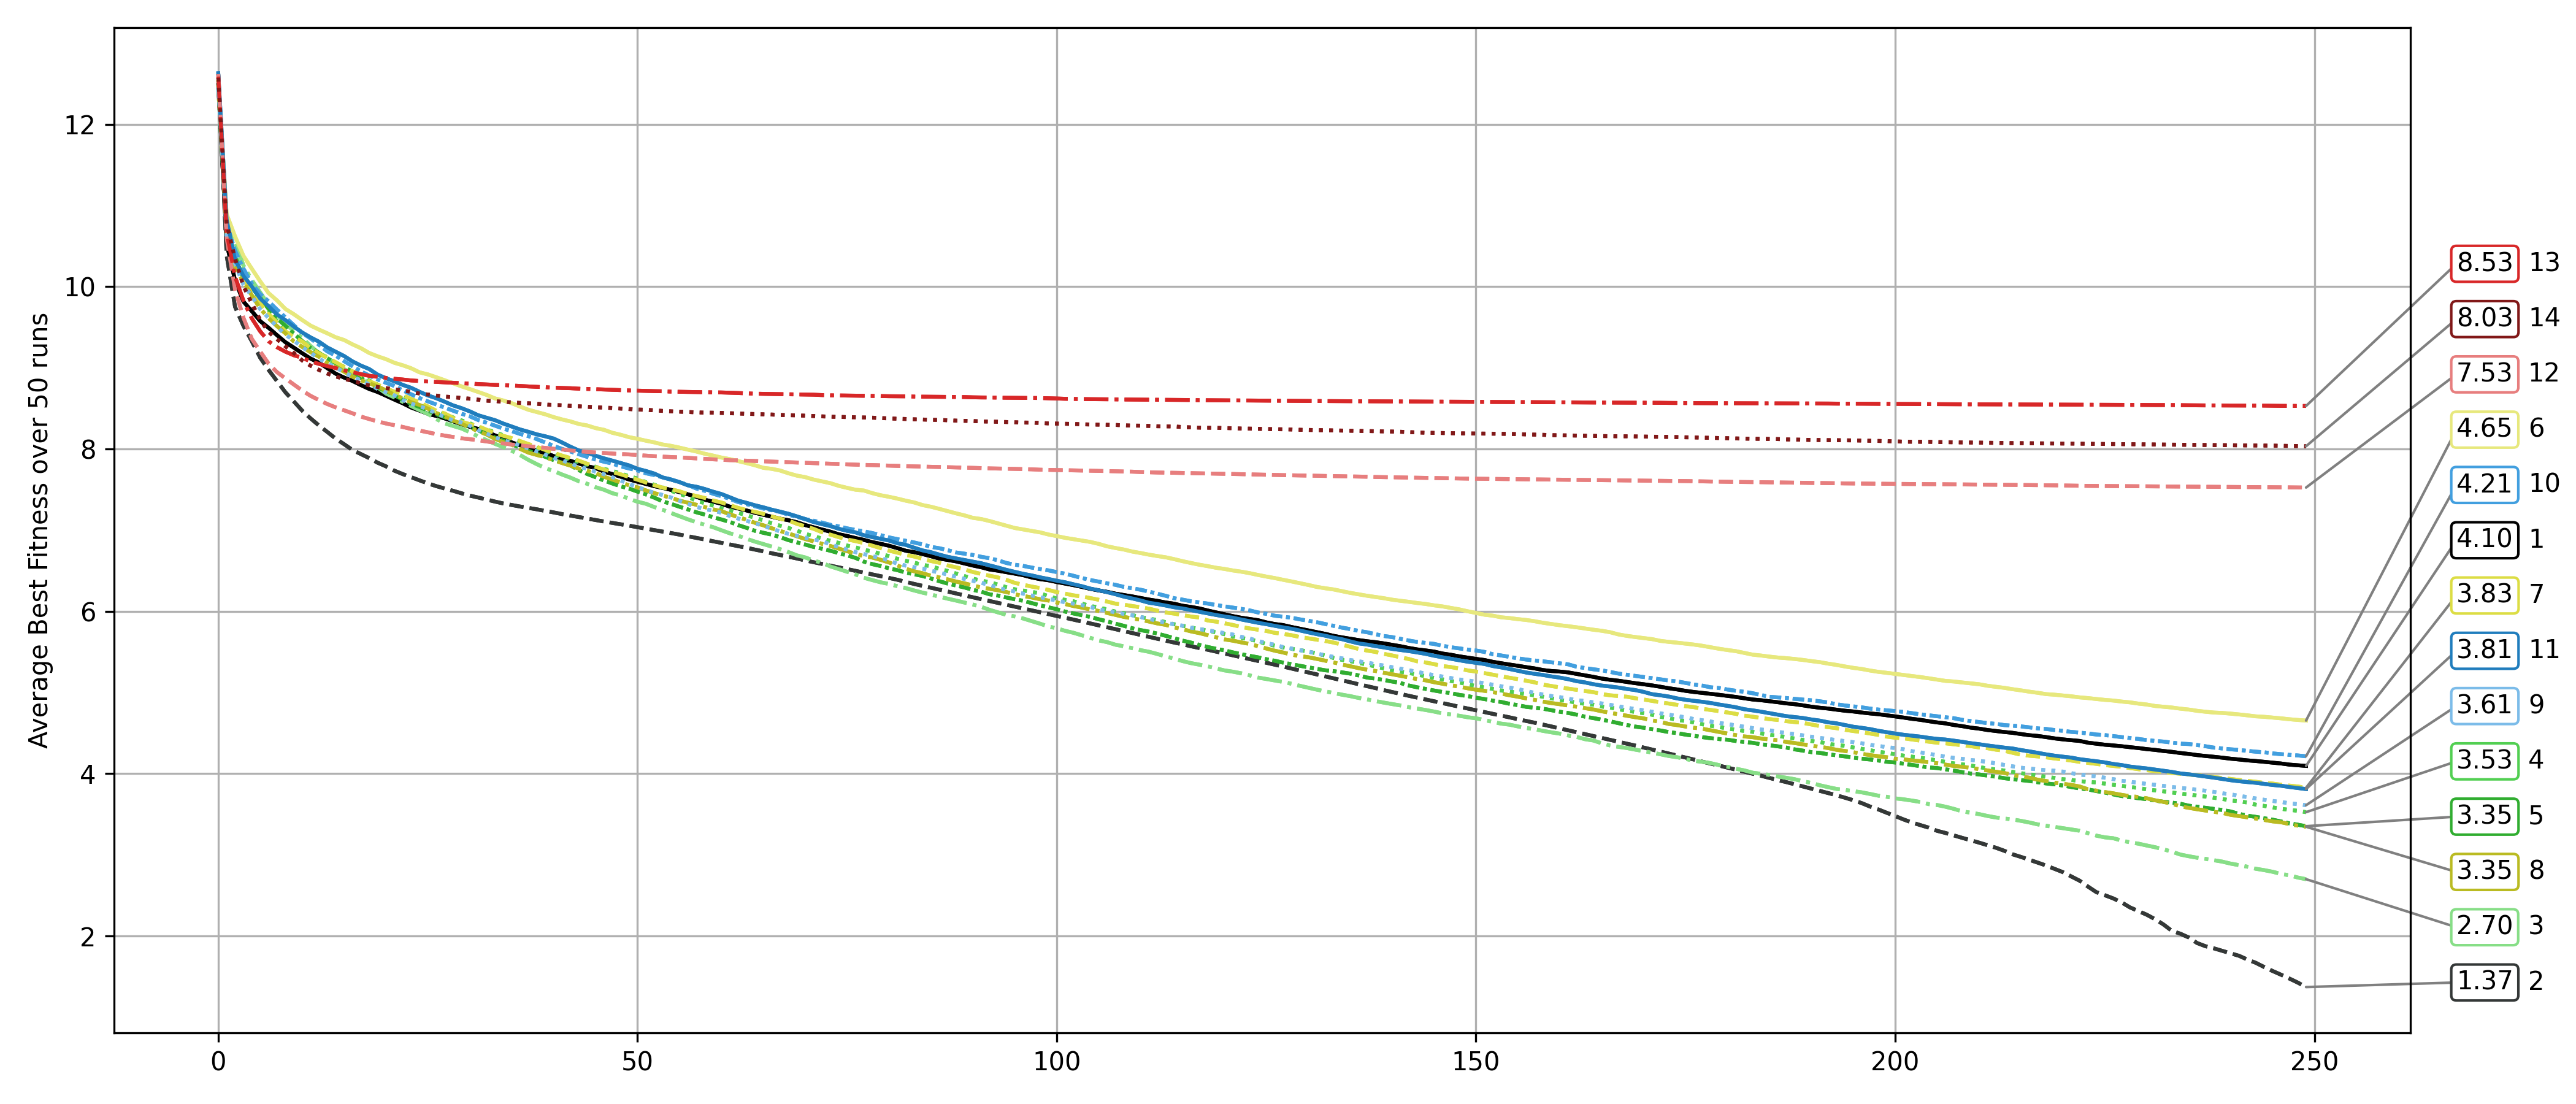
\includegraphics[width=.49\textwidth]{Figures/results/100/Shifted_and_Rotated_HappyCat_All_selected_algorithms_dim100_annot_legend.png}
    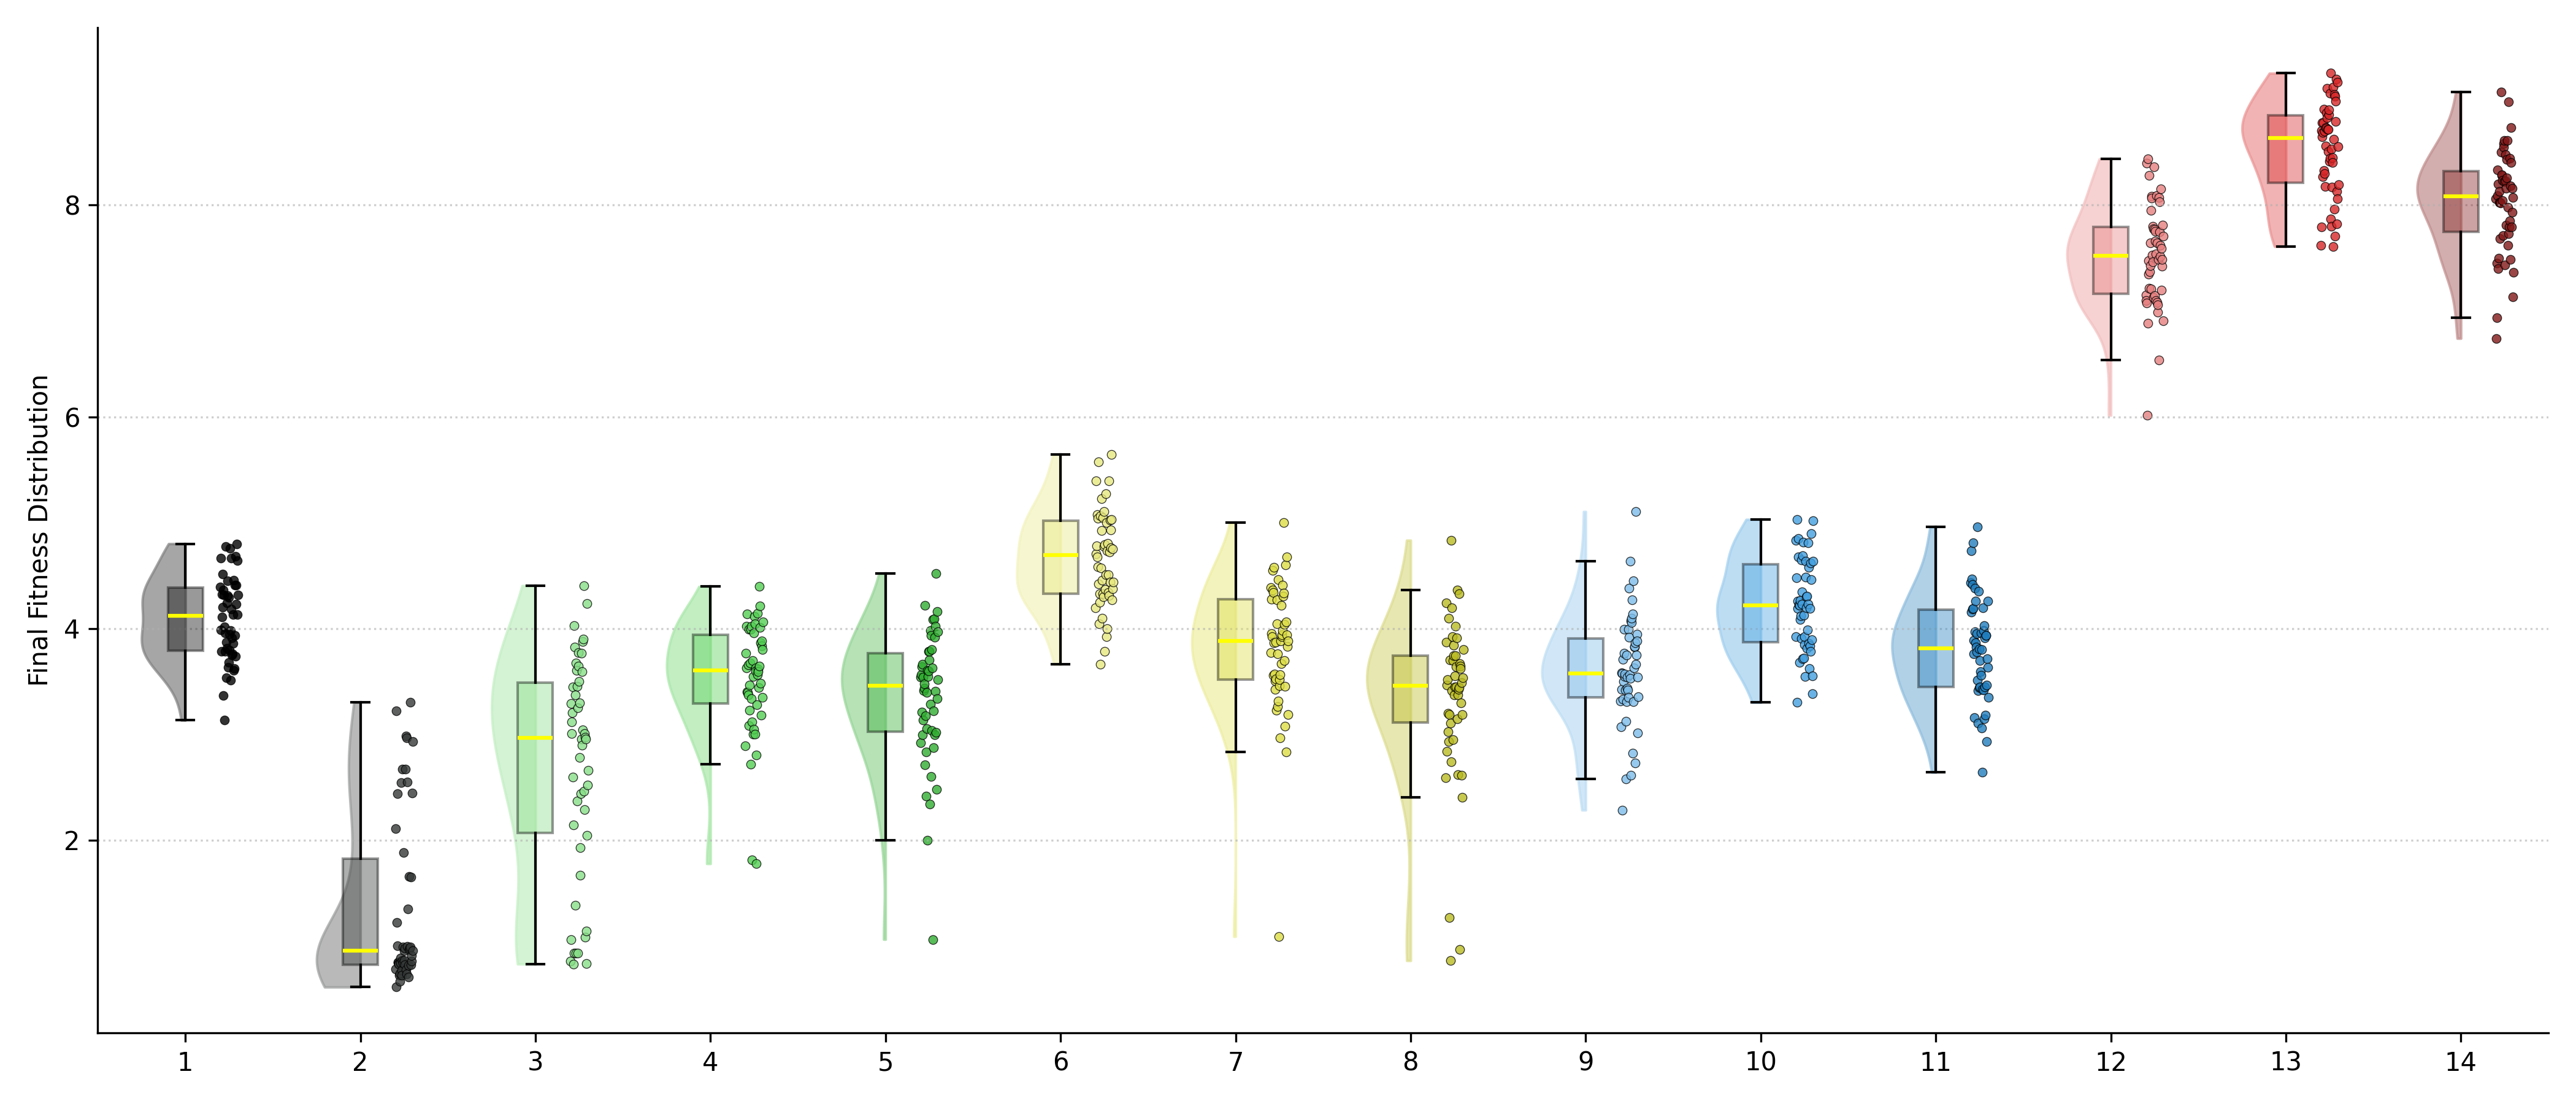
\includegraphics[width=.49\textwidth]{Figures/results/100/Shifted_and_Rotated_HappyCat_all_dim100_raincloud_vertical.png}
    \caption{Shifted and Rotated HappyCat}
\end{subfigure}

\enlargethispage{1\baselineskip}
\captionsetup{list=no}
\caption[Convergence curves and final fitness distribution raincloud plots for 100-dimensional problems]{Convergence curves (left) and final fitness distribution raincloud plots (right) for each tested benchmark problem in the 100-dimensional setting. Algorithms are numbered, line-styled, ordered, and color-coded consistently according to the legend in Figure~\ref{fig:plot_encoding}. Problems plotted on a logarithmic scale are indicated with ``(log)'' following the problem name.}
\end{figure}


% %%%%%%%%%


\begin{figure}[p]\ContinuedFloat
\renewcommand\thesubfigure{C.\arabic{figure}.\arabic{subfigure}} % Local change starts here

    \centering

\begin{subfigure}{1\textwidth}
    \centering
    \includegraphics[width=.49\textwidth]{Figures/results/100/Shifted_and_Rotated_Expanded_Scaffer’s_F6_All_selected_algorithms_dim100_annot_legend.png}
    \includegraphics[width=.49\textwidth]{Figures/results/100/Shifted_and_Rotated_Expanded_Scaffer’s_F6_all_dim100_raincloud_vertical.png}
    \caption{Shifted and Rotated Schaffer F7}
\end{subfigure}

\begin{subfigure}{1\textwidth}
    \centering
    \includegraphics[width=.49\textwidth]{Figures/results/100/Shifted_and_Rotated_Weierstrass_All_selected_algorithms_dim100_annot_legend.png}
    \includegraphics[width=.49\textwidth]{Figures/results/100/Shifted_and_Rotated_Weierstrass_all_dim100_raincloud_vertical.png}
    \caption{Shifted and Rotated Weierstrass}
\end{subfigure}

\begin{subfigure}{1\textwidth}
    \centering
    \includegraphics[width=.49\textwidth]{Figures/results/100/Shubert_N3_All_selected_algorithms_dim100_annot_legend.png}
    \includegraphics[width=.49\textwidth]{Figures/results/100/Shubert_N3_all_dim100_raincloud_vertical.png}
    \caption{Shubert N3}
\end{subfigure}

\begin{subfigure}{1\textwidth}
    \centering
    \includegraphics[width=.49\textwidth]{Figures/results/100/Shubert_N4_All_selected_algorithms_dim100_annot_legend.png}
    \includegraphics[width=.49\textwidth]{Figures/results/100/Shubert_N4_all_dim100_raincloud_vertical.png}
    \caption{Shubert N4}
\end{subfigure}

\begin{subfigure}{1\textwidth}
    \centering
    \includegraphics[width=.49\textwidth]{Figures/results/100/SineEnvelope_All_selected_algorithms_dim100_annot_legend.png}
    \includegraphics[width=.49\textwidth]{Figures/results/100/SineEnvelope_all_dim100_raincloud_vertical.png}
    \caption{Sine Envelope}
\end{subfigure}

\begin{subfigure}{1\textwidth}
    \centering
    \includegraphics[width=.49\textwidth]{Figures/results/100/Stochastic_All_selected_algorithms_dim100_annot_legend.png}
    \includegraphics[width=.49\textwidth]{Figures/results/100/Stochastic_all_dim100_raincloud_vertical.png}
    \caption{Stochastic (log)}
\end{subfigure}

\captionsetup{list=no}
\caption[Convergence curves and final fitness distribution raincloud plots for 100-dimensional problems]{Convergence curves (left) and final fitness distribution raincloud plots (right) for each tested benchmark problem in the 100-dimensional setting. Algorithms are numbered, line-styled, ordered, and color-coded consistently according to the legend in Figure~\ref{fig:plot_encoding}. Problems plotted on a logarithmic scale are indicated with ``(log)'' following the problem name.}
\end{figure}



% %%%%%%%%%


\begin{figure}[H]\ContinuedFloat
\renewcommand\thesubfigure{C.\arabic{figure}.\arabic{subfigure}} % Local change starts here

    \centering

\begin{subfigure}{1\textwidth}
    \centering
    \includegraphics[width=.49\textwidth]{Figures/results/100/StretchedV_All_selected_algorithms_dim100_annot_legend.png}
    \includegraphics[width=.49\textwidth]{Figures/results/100/StretchedV_all_dim100_raincloud_vertical.png}
    \caption{StretchedV (log)}
\end{subfigure}

\begin{subfigure}{1\textwidth}
    \centering
    \includegraphics[width=.49\textwidth]{Figures/results/100/Styblinski–Tang_All_selected_algorithms_dim100_annot_legend.png}
    \includegraphics[width=.49\textwidth]{Figures/results/100/Styblinski–Tang_all_dim100_raincloud_vertical.png}
    \caption{Styblinski–Tang}
\end{subfigure}

\caption[Convergence curves and final fitness distribution raincloud plots for\\100-dimensional problems]{Convergence curves (left) and final fitness distribution raincloud plots (right) for each tested benchmark problem in the 100-dimensional setting. Algorithms are numbered, line-styled, ordered, and color-coded consistently according to the legend in Figure~\ref{fig:plot_encoding}. Problems plotted on a logarithmic scale are indicated with ``(log)'' following the problem name.}
\label{fig:results100}
\end{figure}


% %%%%%%%%%
%%%%%%%%%%%%%%%%%%%%%%%%%%%%%%%%%%%%%%%%%%%%%%%%%%%%%%%%%%%%%%%%%%%%%%%%%%%%
%%%%%%%%%%%%%%%%%%%%%%%%%%%%%%%%%%%%%%%%%%%%%%%%%%%%%%%%%%%%%%%%%%%%%%%%%%%%
%%%%%%%%%%%%%%%%%%%%%%%%%%%%%%%%%%%%%%%%%%%%%%%%%%%%%%%%%%%%%%%%%%%%%%%%%%%%



\vfill
% \vspace{.875em}


\begin{figure}[H]
\renewcommand\thesubfigure{C.\arabic{figure}.\arabic{subfigure}} % Local change starts here

    \centering

    \begin{subfigure}{1\textwidth}
    \centering
    \includegraphics[width=.49\textwidth]{Figures/results/500/Alpine_N1_All_selected_algorithms_dim500_annot_legend.png}
    \includegraphics[width=.49\textwidth]{Figures/results/500/Alpine_N1_all_dim500_raincloud_vertical.png}
    \caption{Alpine N.1 (log)}
\end{subfigure}

\begin{subfigure}{1\textwidth}
    \centering
    \includegraphics[width=.49\textwidth]{Figures/results/500/Crowned_Cross_All_selected_algorithms_dim500_annot_legend.png}
    \includegraphics[width=.49\textwidth]{Figures/results/500/Crowned_Cross_all_dim500_raincloud_vertical.png}
    \caption{Crowned Cross}
\end{subfigure}

\begin{subfigure}{1\textwidth}
    \centering
    \includegraphics[width=.49\textwidth]{Figures/results/500/Egg_Holder_All_selected_algorithms_dim500_annot_legend.png}
    \includegraphics[width=.49\textwidth]{Figures/results/500/Egg_Holder_all_dim500_raincloud_vertical.png}
    \caption{Egg-Holder}
\end{subfigure}

\captionsetup{list=no}
\caption[Convergence curves and final fitness distribution raincloud plots for\\500-dimensional problems]{Convergence curves (left) and final fitness distribution raincloud plots (right) for each tested benchmark problem in the 500-dimensional setting. Algorithms are numbered, line-styled, ordered, and color-coded consistently according to the legend in Figure~\ref{fig:plot_encoding}. Problems plotted on a logarithmic scale are indicated with ``(log)'' following the problem name.}
\end{figure}



% %%%%%%%%%


\begin{figure}[p]\ContinuedFloat
\renewcommand\thesubfigure{C.\arabic{figure}.\arabic{subfigure}} % Local change starts here

    \centering

\begin{subfigure}{1\textwidth}
    \centering
    \includegraphics[width=.49\textwidth]{Figures/results/500/Expanded_Shaffer_All_selected_algorithms_dim500_annot_legend.png}
    \includegraphics[width=.49\textwidth]{Figures/results/500/Expanded_Shaffer_all_dim500_raincloud_vertical.png}
    \caption{Expanded Shaffer}
\end{subfigure}

\begin{subfigure}{1\textwidth}
    \centering
    \includegraphics[width=.49\textwidth]{Figures/results/500/Generalized_Schaffer_N1_All_selected_algorithms_dim500_annot_legend.png}
    \includegraphics[width=.49\textwidth]{Figures/results/500/Generalized_Schaffer_N1_all_dim500_raincloud_vertical.png}
    \caption{Generalized Schaffer N.1}
\end{subfigure}

\begin{subfigure}{1\textwidth}
    \centering
    \includegraphics[width=.49\textwidth]{Figures/results/500/Generalized_Schaffer_N2_All_selected_algorithms_dim500_annot_legend.png}
    \includegraphics[width=.49\textwidth]{Figures/results/500/Generalized_Schaffer_N2_all_dim500_raincloud_vertical.png}
    \caption{Generalized Schaffer N.2}
\end{subfigure}

\begin{subfigure}{1\textwidth}
    \centering
    \includegraphics[width=.49\textwidth]{Figures/results/500/Generalized_Schaffer_N3_All_selected_algorithms_dim500_annot_legend.png}
    \includegraphics[width=.49\textwidth]{Figures/results/500/Generalized_Schaffer_N3_all_dim500_raincloud_vertical.png}
    \caption{Generalized Schaffer N3}
\end{subfigure}

\begin{subfigure}{1\textwidth}
    \centering
    \includegraphics[width=.49\textwidth]{Figures/results/500/Generalized_Schaffer_N4_All_selected_algorithms_dim500_annot_legend.png}
    \includegraphics[width=.49\textwidth]{Figures/results/500/Generalized_Schaffer_N4_all_dim500_raincloud_vertical.png}
    \caption{Generalized Schaffer N4}
\end{subfigure}

\begin{subfigure}{1\textwidth}
    \centering
    \includegraphics[width=.49\textwidth]{Figures/results/500/Generalized_Schmidt–Vetters_All_selected_algorithms_dim500_annot_legend.png}
    \includegraphics[width=.49\textwidth]{Figures/results/500/Generalized_Schmidt–Vetters_all_dim500_raincloud_vertical.png}
    \caption{Generalized Schmidt–Vetters}
\end{subfigure}

\captionsetup{list=no}
\caption[Convergence curves and final fitness distribution raincloud plots for 500-dimensional problems]{Convergence curves (left) and final fitness distribution raincloud plots (right) for each tested benchmark problem in the 500-dimensional setting. Algorithms are numbered, line-styled, ordered, and color-coded consistently according to the legend in Figure~\ref{fig:plot_encoding}. Problems plotted on a logarithmic scale are indicated with ``(log)'' following the problem name.}
\end{figure}



% %%%%%%%%%


\begin{figure}[p]\ContinuedFloat
\renewcommand\thesubfigure{C.\arabic{figure}.\arabic{subfigure}} % Local change starts here

    \centering

\begin{subfigure}{1\textwidth}
    \centering
    \includegraphics[width=.49\textwidth]{Figures/results/500/Lennard_Jones_Minimum_Energy_Cluster_All_selected_algorithms_dim500_annot_legend.png}
    \includegraphics[width=.49\textwidth]{Figures/results/500/Lennard_Jones_Minimum_Energy_Cluster_all_dim500_raincloud_vertical.png}
    \caption{Lennard-Jones Minimum Energy Cluster}
\end{subfigure}

\begin{subfigure}{1\textwidth}
    \centering
    \includegraphics[width=.49\textwidth]{Figures/results/500/Michalewicz_All_selected_algorithms_dim500_annot_legend.png}
    \includegraphics[width=.49\textwidth]{Figures/results/500/Michalewicz_all_dim500_raincloud_vertical.png}
    \caption{Michalewicz}
\end{subfigure}

\begin{subfigure}{1\textwidth}
    \centering
    \includegraphics[width=.49\textwidth]{Figures/results/500/Mishra_N3_All_selected_algorithms_dim500_annot_legend.png}
    \includegraphics[width=.49\textwidth]{Figures/results/500/Mishra_N3_all_dim500_raincloud_vertical.png}
    \caption{Mishra N3}
\end{subfigure}

\begin{subfigure}{1\textwidth}
    \centering
    \includegraphics[width=.49\textwidth]{Figures/results/500/Mishra_N4_All_selected_algorithms_dim500_annot_legend.png}
    \includegraphics[width=.49\textwidth]{Figures/results/500/Mishra_N4_all_dim500_raincloud_vertical.png}
    \caption{Mishra N4}
\end{subfigure}

\begin{subfigure}{1\textwidth}
    \centering
    \includegraphics[width=.49\textwidth]{Figures/results/500/Modified_Rosenbrock_No.02___Hollow_Ground_Bent_Knife_Edge_All_selected_algorithms_dim500_annot_legend.png}
    \includegraphics[width=.49\textwidth]{Figures/results/500/Modified_Rosenbrock_No.02___Hollow_Ground_Bent_Knife_Edge_all_dim500_raincloud_vertical.png}
    \caption{Modified Rosenbrock N.2 (log)}
\end{subfigure}

\begin{subfigure}{1\textwidth}
    \centering
    \includegraphics[width=.49\textwidth]{Figures/results/500/Rotated_Bent_Cigar_All_selected_algorithms_dim500_annot_legend.png}
    \includegraphics[width=.49\textwidth]{Figures/results/500/Rotated_Bent_Cigar_all_dim500_raincloud_vertical.png}
    \caption{Rotated Bent Cigar (log)}
\end{subfigure}


\captionsetup{list=no}
\caption[Convergence curves and final fitness distribution raincloud plots for 500-dimensional problems]{Convergence curves (left) and final fitness distribution raincloud plots (right) for each tested benchmark problem in the 500-dimensional setting. Algorithms are numbered, line-styled, ordered, and color-coded consistently according to the legend in Figure~\ref{fig:plot_encoding}. Problems plotted on a logarithmic scale are indicated with ``(log)'' following the problem name.}
\end{figure}



% % %%%%%%%%%


\begin{figure}[p]\ContinuedFloat
\renewcommand\thesubfigure{C.\arabic{figure}.\arabic{subfigure}} % Local change starts here

    \centering


\begin{subfigure}{1\textwidth}
    \centering
    \includegraphics[width=.49\textwidth]{Figures/results/500/Rotated_Discus_All_selected_algorithms_dim500_annot_legend.png}
    \includegraphics[width=.49\textwidth]{Figures/results/500/Rotated_Discus_all_dim500_raincloud_vertical.png}
    \caption{Rotated Discus (log)}
\end{subfigure}

\begin{subfigure}{1\textwidth}
    \centering
    \includegraphics[width=.49\textwidth]{Figures/results/500/Rotated_High_Conditioned_Elliptic_All_selected_algorithms_dim500_annot_legend.png}
    \includegraphics[width=.49\textwidth]{Figures/results/500/Rotated_High_Conditioned_Elliptic_all_dim500_raincloud_vertical.png}
    \caption{Rotated High Conditioned Elliptic (log)}
\end{subfigure}

\begin{subfigure}{1\textwidth}
    \centering
    \includegraphics[width=.49\textwidth]{Figures/results/500/Salomon_All_selected_algorithms_dim500_annot_legend.png}
    \includegraphics[width=.49\textwidth]{Figures/results/500/Salomon_all_dim500_raincloud_vertical.png}
    \caption{Salomon (log)}
\end{subfigure}

\begin{subfigure}{1\textwidth}
    \centering
    \includegraphics[width=.49\textwidth]{Figures/results/500/Schwefel_N20_All_selected_algorithms_dim500_annot_legend.png}
    \includegraphics[width=.49\textwidth]{Figures/results/500/Schwefel_N20_all_dim500_raincloud_vertical.png}
    \caption{Schwefel N.20}
\end{subfigure}

\begin{subfigure}{1\textwidth}
    \centering
    \includegraphics[width=.49\textwidth]{Figures/results/500/Schwefel_N36_All_selected_algorithms_dim500_annot_legend.png}
    \includegraphics[width=.49\textwidth]{Figures/results/500/Schwefel_N36_all_dim500_raincloud_vertical.png}
    \caption{Schwefel N36}
\end{subfigure}

\begin{subfigure}{1\textwidth}
    \centering
    \includegraphics[width=.49\textwidth]{Figures/results/500/Schwefel_N6_All_selected_algorithms_dim500_annot_legend.png}
    \includegraphics[width=.49\textwidth]{Figures/results/500/Schwefel_N6_all_dim500_raincloud_vertical.png}
    \caption{Schwefel N6 (log)}
\end{subfigure}


\captionsetup{list=no}
\caption[Convergence curves and final fitness distribution raincloud plots for 500-dimensional problems]{Convergence curves (left) and final fitness distribution raincloud plots (right) for each tested benchmark problem in the 500-dimensional setting. Algorithms are numbered, line-styled, ordered, and color-coded consistently according to the legend in Figure~\ref{fig:plot_encoding}. Problems plotted on a logarithmic scale are indicated with ``(log)'' following the problem name.}
\end{figure}



% % %%%%%%%%%


\begin{figure}[p]\ContinuedFloat
\renewcommand\thesubfigure{C.\arabic{figure}.\arabic{subfigure}} % Local change starts here

    \centering
\begin{subfigure}{1\textwidth}
    \centering
    \includegraphics[width=.49\textwidth]{Figures/results/500/Shifted_Schwefel_All_selected_algorithms_dim500_annot_legend.png}
    \includegraphics[width=.49\textwidth]{Figures/results/500/Shifted_Schwefel_all_dim500_raincloud_vertical.png}
    \caption{Shifted Schwefel}
\end{subfigure}

\begin{subfigure}{1\textwidth}
    \centering
    \includegraphics[width=.49\textwidth]{Figures/results/500/Shifted_and_Rotated_HGBat_All_selected_algorithms_dim500_annot_legend.png}
    \includegraphics[width=.49\textwidth]{Figures/results/500/Shifted_and_Rotated_HGBat_all_dim500_raincloud_vertical.png}
    \caption{Shifted and Rotated HGBat}
\end{subfigure}

\begin{subfigure}{1\textwidth}
    \centering
    \includegraphics[width=.49\textwidth]{Figures/results/500/Shifted_and_Rotated_HappyCat_All_selected_algorithms_dim500_annot_legend.png}
    \includegraphics[width=.49\textwidth]{Figures/results/500/Shifted_and_Rotated_HappyCat_all_dim500_raincloud_vertical.png}
    \caption{Shifted and Rotated HappyCat}
\end{subfigure}

\begin{subfigure}{1\textwidth}
    \centering
    \includegraphics[width=.49\textwidth]{Figures/results/500/Shifted_and_Rotated_Expanded_Scaffer’s_F6_All_selected_algorithms_dim500_annot_legend.png}
    \includegraphics[width=.49\textwidth]{Figures/results/500/Shifted_and_Rotated_Expanded_Scaffer’s_F6_all_dim500_raincloud_vertical.png}
    \caption{Shifted and Rotated Schaffer F7}
\end{subfigure}

\begin{subfigure}{1\textwidth}
    \centering
    \includegraphics[width=.49\textwidth]{Figures/results/500/Shifted_and_Rotated_Weierstrass_All_selected_algorithms_dim500_annot_legend.png}
    \includegraphics[width=.49\textwidth]{Figures/results/500/Shifted_and_Rotated_Weierstrass_all_dim500_raincloud_vertical.png}
    \caption{Shifted and Rotated Weierstrass}
\end{subfigure}

\begin{subfigure}{1\textwidth}
    \centering
    \includegraphics[width=.49\textwidth]{Figures/results/500/Shubert_N3_All_selected_algorithms_dim500_annot_legend.png}
    \includegraphics[width=.49\textwidth]{Figures/results/500/Shubert_N3_all_dim500_raincloud_vertical.png}
    \caption{Shubert N3}
\end{subfigure}

\captionsetup{list=no}
\caption[Convergence curves and final fitness distribution raincloud plots for 500-dimensional problems]{Convergence curves (left) and final fitness distribution raincloud plots (right) for each tested benchmark problem in the 500-dimensional setting. Algorithms are numbered, line-styled, ordered, and color-coded consistently according to the legend in Figure~\ref{fig:plot_encoding}. Problems plotted on a logarithmic scale are indicated with ``(log)'' following the problem name.}
\end{figure}



% % %%%%%%%%%


\begin{figure}[p]\ContinuedFloat
\renewcommand\thesubfigure{C.\arabic{figure}.\arabic{subfigure}} % Local change starts here

    \centering



\begin{subfigure}{1\textwidth}
    \centering
    \includegraphics[width=.49\textwidth]{Figures/results/500/Shubert_N4_All_selected_algorithms_dim500_annot_legend.png}
    \includegraphics[width=.49\textwidth]{Figures/results/500/Shubert_N4_all_dim500_raincloud_vertical.png}
    \caption{Shubert N4}
\end{subfigure}

\begin{subfigure}{1\textwidth}
    \centering
    \includegraphics[width=.49\textwidth]{Figures/results/500/SineEnvelope_All_selected_algorithms_dim500_annot_legend.png}
    \includegraphics[width=.49\textwidth]{Figures/results/500/SineEnvelope_all_dim500_raincloud_vertical.png}
    \caption{SineEnvelope}
\end{subfigure}

\begin{subfigure}{1\textwidth}
    \centering
    \includegraphics[width=.49\textwidth]{Figures/results/500/Stochastic_All_selected_algorithms_dim500_annot_legend.png}
    \includegraphics[width=.49\textwidth]{Figures/results/500/Stochastic_all_dim500_raincloud_vertical.png}
    \caption{Stochastic (log)}
\end{subfigure}

\begin{subfigure}{1\textwidth}
    \centering
    \includegraphics[width=.49\textwidth]{Figures/results/500/StretchedV_All_selected_algorithms_dim500_annot_legend.png}
    \includegraphics[width=.49\textwidth]{Figures/results/500/StretchedV_all_dim500_raincloud_vertical.png}
    \caption{StretchedV (log)}
\end{subfigure}

\begin{subfigure}{1\textwidth}
    \centering
    \includegraphics[width=.49\textwidth]{Figures/results/500/Styblinski–Tang_All_selected_algorithms_dim500_annot_legend.png}
    \includegraphics[width=.49\textwidth]{Figures/results/500/Styblinski–Tang_all_dim500_raincloud_vertical.png}
    \caption{Styblinski–Tang}
\end{subfigure}



% \captionsetup{list=no}
\caption[Convergence curves and final fitness distribution raincloud plots for\\500-dimensional problems]{Convergence curves (left) and final fitness distribution raincloud plots (right) for each tested benchmark problem in the 500-dimensional setting. Algorithms are numbered, line-styled, ordered, and color-coded consistently according to the legend in Figure~\ref{fig:plot_encoding}. Problems plotted on a logarithmic scale are indicated with ``(log)'' following the problem name.}
\label{fig:results500}
\end{figure}


%%%%%%%%%%%%%%%%%%%%%%%%%%%%%%%%%%%%%%%%%%%%%%%%%%%%%%%%%%%%%%%%%%%%%%%%%%%%%%%%%%%%%%%%%%%%%%%%%%%%%%%%
%%%%%%%%%%%%%%%%%%%%%%%%%%%%%%%%%%%%%%%%%%%%%%%%%%%%%%%%%%%%%%%%%%%%%%%%%%%%%%%%%%%%%%%%%%%%%%%%%%%%%%%%
%%%%%%%%%%%%%%%%%%%%%%%%%%%%%%%%%%%%%%%%%%%%%%%%%%%%%%%%%%%%%%%%%%%%%%%%%%%%%%%%%%%%%%%%%%%%%%%%%%%%%%%%
% % %%%%%%%%%


\begin{figure}[p]
\renewcommand\thesubfigure{C.\arabic{figure}.\arabic{subfigure}} % Local change starts here
    \centering

    \begin{subfigure}{1\textwidth}
    \centering
    \includegraphics[width=.49\textwidth]{Figures/results/1000/Alpine_N1_All_selected_algorithms_dim1000_annot_legend.png}
    \includegraphics[width=.49\textwidth]{Figures/results/1000/Alpine_N1_all_dim1000_raincloud_vertical.png}
    \caption{Alpine N.1 (log)}
\end{subfigure}

\begin{subfigure}{1\textwidth}
    \centering
    \includegraphics[width=.49\textwidth]{Figures/results/1000/Crowned_Cross_All_selected_algorithms_dim1000_annot_legend.png}
    \includegraphics[width=.49\textwidth]{Figures/results/1000/Crowned_Cross_all_dim1000_raincloud_vertical.png}
    \caption{Crowned Cross}
\end{subfigure}

\begin{subfigure}{1\textwidth}
    \centering
    \includegraphics[width=.49\textwidth]{Figures/results/1000/Egg_Holder_All_selected_algorithms_dim1000_annot_legend.png}
    \includegraphics[width=.49\textwidth]{Figures/results/1000/Egg_Holder_all_dim1000_raincloud_vertical.png}
    \caption{Egg-Holder}
\end{subfigure}

\begin{subfigure}{1\textwidth}
    \centering
    \includegraphics[width=.49\textwidth]{Figures/results/1000/Expanded_Shaffer_All_selected_algorithms_dim1000_annot_legend.png}
    \includegraphics[width=.49\textwidth]{Figures/results/1000/Expanded_Shaffer_all_dim1000_raincloud_vertical.png}
    \caption{Expanded Shaffer}
\end{subfigure}

\begin{subfigure}{1\textwidth}
    \centering
    \includegraphics[width=.49\textwidth]{Figures/results/1000/Generalized_Schaffer_N1_All_selected_algorithms_dim1000_annot_legend.png}
    \includegraphics[width=.49\textwidth]{Figures/results/1000/Generalized_Schaffer_N1_all_dim1000_raincloud_vertical.png}
    \caption{Generalized Schaffer N.1}
\end{subfigure}

\begin{subfigure}{1\textwidth}
    \centering
    \includegraphics[width=.49\textwidth]{Figures/results/1000/Generalized_Schaffer_N2_All_selected_algorithms_dim1000_annot_legend.png}
    \includegraphics[width=.49\textwidth]{Figures/results/1000/Generalized_Schaffer_N2_all_dim1000_raincloud_vertical.png}
    \caption{Generalized Schaffer N.2}
\end{subfigure}

\captionsetup{list=no}
\caption[Convergence curves and final fitness distribution raincloud plots for 1000-dimensional problems]{Convergence curves (left) and final fitness distribution raincloud plots (right) for each tested benchmark problem in the 1000-dimensional setting. Algorithms are numbered, line-styled, ordered, and color-coded consistently according to the legend in Figure~\ref{fig:plot_encoding}. Problems plotted on a logarithmic scale are indicated with ``(log)'' following the problem name.}
\end{figure}



% % %%%%%%%%%


\begin{figure}[p]\ContinuedFloat
\renewcommand\thesubfigure{C.\arabic{figure}.\arabic{subfigure}} % Local change starts here
    \centering

\begin{subfigure}{1\textwidth}
    \centering
    \includegraphics[width=.49\textwidth]{Figures/results/1000/Generalized_Schaffer_N3_All_selected_algorithms_dim1000_annot_legend.png}
    \includegraphics[width=.49\textwidth]{Figures/results/1000/Generalized_Schaffer_N3_all_dim1000_raincloud_vertical.png}
    \caption{Generalized Schaffer N3}
\end{subfigure}

\begin{subfigure}{1\textwidth}
    \centering
    \includegraphics[width=.49\textwidth]{Figures/results/1000/Generalized_Schaffer_N4_All_selected_algorithms_dim1000_annot_legend.png}
    \includegraphics[width=.49\textwidth]{Figures/results/1000/Generalized_Schaffer_N4_all_dim1000_raincloud_vertical.png}
    \caption{Generalized Schaffer N4}
\end{subfigure}

\begin{subfigure}{1\textwidth}
    \centering
    \includegraphics[width=.49\textwidth]{Figures/results/1000/Generalized_Schmidt–Vetters_All_selected_algorithms_dim1000_annot_legend.png}
    \includegraphics[width=.49\textwidth]{Figures/results/1000/Generalized_Schmidt–Vetters_all_dim1000_raincloud_vertical.png}
    \caption{Generalized Schmidt–Vetters}
\end{subfigure}

\begin{subfigure}{1\textwidth}
    \centering
    \includegraphics[width=.49\textwidth]{Figures/results/1000/Lennard_Jones_Minimum_Energy_Cluster_All_selected_algorithms_dim1000_annot_legend.png}
    \includegraphics[width=.49\textwidth]{Figures/results/1000/Lennard_Jones_Minimum_Energy_Cluster_all_dim1000_raincloud_vertical.png}
    \caption{Lennard-Jones Minimum Energy Cluster}
\end{subfigure}

\begin{subfigure}{1\textwidth}
    \centering
    \includegraphics[width=.49\textwidth]{Figures/results/1000/Michalewicz_All_selected_algorithms_dim1000_annot_legend.png}
    \includegraphics[width=.49\textwidth]{Figures/results/1000/Michalewicz_all_dim1000_raincloud_vertical.png}
    \caption{Michalewicz}
\end{subfigure}

\begin{subfigure}{1\textwidth}
    \centering
    \includegraphics[width=.49\textwidth]{Figures/results/1000/Mishra_N3_All_selected_algorithms_dim1000_annot_legend.png}
    \includegraphics[width=.49\textwidth]{Figures/results/1000/Mishra_N3_all_dim1000_raincloud_vertical.png}
    \caption{Mishra N3}
\end{subfigure}

\captionsetup{list=no}
\caption[Convergence curves and final fitness distribution raincloud plots for 1000-dimensional problems]{Convergence curves (left) and final fitness distribution raincloud plots (right) for each tested benchmark problem in the 1000-dimensional setting. Algorithms are numbered, line-styled, ordered, and color-coded consistently according to the legend in Figure~\ref{fig:plot_encoding}. Problems plotted on a logarithmic scale are indicated with ``(log)'' following the problem name.}
\end{figure}



% % %%%%%%%%%


\begin{figure}[p]\ContinuedFloat
\renewcommand\thesubfigure{C.\arabic{figure}.\arabic{subfigure}} % Local change starts here
    \centering

\begin{subfigure}{1\textwidth}
    \centering
    \includegraphics[width=.49\textwidth]{Figures/results/1000/Mishra_N4_All_selected_algorithms_dim1000_annot_legend.png}
    \includegraphics[width=.49\textwidth]{Figures/results/1000/Mishra_N4_all_dim1000_raincloud_vertical.png}
    \caption{Mishra N4}
\end{subfigure}

\begin{subfigure}{1\textwidth}
    \centering
    \includegraphics[width=.49\textwidth]{Figures/results/1000/Modified_Rosenbrock_No.02___Hollow_Ground_Bent_Knife_Edge_All_selected_algorithms_dim1000_annot_legend.png}
    \includegraphics[width=.49\textwidth]{Figures/results/1000/Modified_Rosenbrock_No.02___Hollow_Ground_Bent_Knife_Edge_all_dim1000_raincloud_vertical.png}
    \caption{Modified Rosenbrock N.2 (log)}
\end{subfigure}

\begin{subfigure}{1\textwidth}
    \centering
    \includegraphics[width=.49\textwidth]{Figures/results/1000/Rotated_Bent_Cigar_All_selected_algorithms_dim1000_annot_legend.png}
    \includegraphics[width=.49\textwidth]{Figures/results/1000/Rotated_Bent_Cigar_all_dim1000_raincloud_vertical.png}
    \caption{Rotated Bent Cigar (log)}
\end{subfigure}

\begin{subfigure}{1\textwidth}
    \centering
    \includegraphics[width=.49\textwidth]{Figures/results/1000/Rotated_Discus_All_selected_algorithms_dim1000_annot_legend.png}
    \includegraphics[width=.49\textwidth]{Figures/results/1000/Rotated_Discus_all_dim1000_raincloud_vertical.png}
    \caption{Rotated Discus (log)}
\end{subfigure}

\begin{subfigure}{1\textwidth}
    \centering
    \includegraphics[width=.49\textwidth]{Figures/results/1000/Rotated_High_Conditioned_Elliptic_All_selected_algorithms_dim1000_annot_legend.png}
    \includegraphics[width=.49\textwidth]{Figures/results/1000/Rotated_High_Conditioned_Elliptic_all_dim1000_raincloud_vertical.png}
    \caption{Rotated High Conditioned Elliptic (log)}
\end{subfigure}

\begin{subfigure}{1\textwidth}
    \centering
    \includegraphics[width=.49\textwidth]{Figures/results/1000/Salomon_All_selected_algorithms_dim1000_annot_legend.png}
    \includegraphics[width=.49\textwidth]{Figures/results/1000/Salomon_all_dim1000_raincloud_vertical.png}
    \caption{Salomon (log)}
\end{subfigure}

\captionsetup{list=no}
\caption[Convergence curves and final fitness distribution raincloud plots for 1000-dimensional problems]{Convergence curves (left) and final fitness distribution raincloud plots (right) for each tested benchmark problem in the 1000-dimensional setting. Algorithms are numbered, line-styled, ordered, and color-coded consistently according to the legend in Figure~\ref{fig:plot_encoding}. Problems plotted on a logarithmic scale are indicated with ``(log)'' following the problem name.}
\end{figure}



% % %%%%%%%%%


\begin{figure}[p]\ContinuedFloat
\renewcommand\thesubfigure{C.\arabic{figure}.\arabic{subfigure}} % Local change starts here
    \centering

\begin{subfigure}{1\textwidth}
    \centering
    \includegraphics[width=.49\textwidth]{Figures/results/1000/Schwefel_N20_All_selected_algorithms_dim1000_annot_legend.png}
    \includegraphics[width=.49\textwidth]{Figures/results/1000/Schwefel_N20_all_dim1000_raincloud_vertical.png}
    \caption{Schwefel N.20}
\end{subfigure}

\begin{subfigure}{1\textwidth}
    \centering
    \includegraphics[width=.49\textwidth]{Figures/results/1000/Schwefel_N36_All_selected_algorithms_dim1000_annot_legend.png}
    \includegraphics[width=.49\textwidth]{Figures/results/1000/Schwefel_N36_all_dim1000_raincloud_vertical.png}
    \caption{Schwefel N36}
\end{subfigure}

\begin{subfigure}{1\textwidth}
    \centering
    \includegraphics[width=.49\textwidth]{Figures/results/1000/Schwefel_N6_All_selected_algorithms_dim1000_annot_legend.png}
    \includegraphics[width=.49\textwidth]{Figures/results/1000/Schwefel_N6_all_dim1000_raincloud_vertical.png}
    \caption{Schwefel N6 (log)}
\end{subfigure}

\begin{subfigure}{1\textwidth}
    \centering
    \includegraphics[width=.49\textwidth]{Figures/results/1000/Shifted_Schwefel_All_selected_algorithms_dim1000_annot_legend.png}
    \includegraphics[width=.49\textwidth]{Figures/results/1000/Shifted_Schwefel_all_dim1000_raincloud_vertical.png}
    \caption{Shifted Schwefel}
\end{subfigure}

\begin{subfigure}{1\textwidth}
    \centering
    \includegraphics[width=.49\textwidth]{Figures/results/1000/Shifted_and_Rotated_HGBat_All_selected_algorithms_dim1000_annot_legend.png}
    \includegraphics[width=.49\textwidth]{Figures/results/1000/Shifted_and_Rotated_HGBat_all_dim1000_raincloud_vertical.png}
    \caption{Shifted and Rotated HGBat}
\end{subfigure}

\begin{subfigure}{1\textwidth}
    \centering
    \includegraphics[width=.49\textwidth]{Figures/results/1000/Shifted_and_Rotated_HappyCat_All_selected_algorithms_dim1000_annot_legend.png}
    \includegraphics[width=.49\textwidth]{Figures/results/1000/Shifted_and_Rotated_HappyCat_all_dim1000_raincloud_vertical.png}
    \caption{Shifted and Rotated HappyCat}
\end{subfigure}

\captionsetup{list=no}
\caption[Convergence curves and final fitness distribution raincloud plots for 1000-dimensional problems]{Convergence curves (left) and final fitness distribution raincloud plots (right) for each tested benchmark problem in the 1000-dimensional setting. Algorithms are numbered, line-styled, ordered, and color-coded consistently according to the legend in Figure~\ref{fig:plot_encoding}. Problems plotted on a logarithmic scale are indicated with ``(log)'' following the problem name.}
\end{figure}



% % %%%%%%%%%


\begin{figure}[p]\ContinuedFloat
\renewcommand\thesubfigure{C.\arabic{figure}.\arabic{subfigure}} % Local change starts here
    \centering

\begin{subfigure}{1\textwidth}
    \centering
    \includegraphics[width=.49\textwidth]{Figures/results/1000/Shifted_and_Rotated_Expanded_Scaffer’s_F6_All_selected_algorithms_dim1000_annot_legend.png}
    \includegraphics[width=.49\textwidth]{Figures/results/1000/Shifted_and_Rotated_Expanded_Scaffer’s_F6_all_dim1000_raincloud_vertical.png}
    \caption{Shifted and Rotated Schaffer F7}
\end{subfigure}

\begin{subfigure}{1\textwidth}
    \centering
    \includegraphics[width=.49\textwidth]{Figures/results/1000/Shifted_and_Rotated_Weierstrass_All_selected_algorithms_dim1000_annot_legend.png}
    \includegraphics[width=.49\textwidth]{Figures/results/1000/Shifted_and_Rotated_Weierstrass_all_dim1000_raincloud_vertical.png}
    \caption{Shifted and Rotated Weierstrass}
\end{subfigure}

\begin{subfigure}{1\textwidth}
    \centering
    \includegraphics[width=.49\textwidth]{Figures/results/1000/Shubert_N3_All_selected_algorithms_dim1000_annot_legend.png}
    \includegraphics[width=.49\textwidth]{Figures/results/1000/Shubert_N3_all_dim1000_raincloud_vertical.png}
    \caption{Shubert N3}
\end{subfigure}

\begin{subfigure}{1\textwidth}
    \centering
    \includegraphics[width=.49\textwidth]{Figures/results/1000/Shubert_N4_All_selected_algorithms_dim1000_annot_legend.png}
    \includegraphics[width=.49\textwidth]{Figures/results/1000/Shubert_N4_all_dim1000_raincloud_vertical.png}
    \caption{Shubert N4}
\end{subfigure}

\begin{subfigure}{1\textwidth}
    \centering
    \includegraphics[width=.49\textwidth]{Figures/results/1000/SineEnvelope_All_selected_algorithms_dim1000_annot_legend.png}
    \includegraphics[width=.49\textwidth]{Figures/results/1000/SineEnvelope_all_dim1000_raincloud_vertical.png}
    \caption{SineEnvelope}
\end{subfigure}

\begin{subfigure}{1\textwidth}
    \centering
    \includegraphics[width=.49\textwidth]{Figures/results/1000/Stochastic_All_selected_algorithms_dim1000_annot_legend.png}
    \includegraphics[width=.49\textwidth]{Figures/results/1000/Stochastic_all_dim1000_raincloud_vertical.png}
    \caption{Stochastic (log)}
\end{subfigure}


\captionsetup{list=no}
\caption[Convergence curves and final fitness distribution raincloud plots for 1000-dimensional problems]{Convergence curves (left) and final fitness distribution raincloud plots (right) for each tested benchmark problem in the 1000-dimensional setting. Algorithms are numbered, line-styled, ordered, and color-coded consistently according to the legend in Figure~\ref{fig:plot_encoding}. Problems plotted on a logarithmic scale are indicated with ``(log)'' following the problem name.}
\end{figure}



% % %%%%%%%%%


\begin{figure}[H]\ContinuedFloat
\renewcommand\thesubfigure{C.\arabic{figure}.\arabic{subfigure}}
    \centering

\begin{subfigure}{1\textwidth}
    \centering
    \includegraphics[width=.49\textwidth]{Figures/results/1000/StretchedV_All_selected_algorithms_dim1000_annot_legend.png}
    \includegraphics[width=.49\textwidth]{Figures/results/1000/StretchedV_all_dim1000_raincloud_vertical.png}
    \caption{StretchedV (log)}
\end{subfigure}

\begin{subfigure}{1\textwidth}
    \centering
    \includegraphics[width=.49\textwidth]{Figures/results/1000/Styblinski–Tang_All_selected_algorithms_dim1000_annot_legend.png}
    \includegraphics[width=.49\textwidth]{Figures/results/1000/Styblinski–Tang_all_dim1000_raincloud_vertical.png}
    \caption{Styblinski–Tang}
\end{subfigure}


% \captionsetup{list=no}
\caption[Convergence curves and final fitness distribution raincloud plots for\\1000-dimensional problems]{Convergence curves (left) and final fitness distribution raincloud plots (right) for each tested benchmark problem in the 1000-dimensional setting. Algorithms are numbered, line-styled, ordered, and color-coded consistently according to the legend in Figure~\ref{fig:plot_encoding}. Problems plotted on a logarithmic scale are indicated with ``(log)'' following the problem name.}
\label{fig:results1000}
\end{figure}



% % %%%%%%%%%


% % \begin{figure}[p]
% %     \centering


% % \captionsetup{list=no}
% % \caption[Parallel coordinates plots of parameter configurations]{Parallel coordinates plots showing the distribution of  parameter configurations, colored by their average objective value.}
% % \end{figure}

